\documentclass[oneside,authoryear,spanish,a4paper]{ezthesis}
%\documentclass[oneside,authoryear,draft,spanish]{ezthesis}
%\documentclass[oneside,authoryear,draftmarks,spanish]{ezthesis}
%% # Opciones disponibles para el documento #
%%
%% Las opciones con un (*) son las opciones predeterminadas.
%%
%% Modo de compilar:
%%   draft            - borrador con marcas de fecha y sin im'agenes
%%   draftmarks       - borrador con marcas de fecha y con im'agenes
%%   final (*)        - version final de la tesis
%%
%% Tama'no de papel:
%%   letterpaper (*)  - tama'no carta (Am'erica)
%%   a4paper          - tama'no A4    (Europa)
%%
%% Formato de impresi'on:
%%   oneside          - hojas impresas por un solo lado
%%   twoside (*)      - hijas impresas por ambos lados
%%
%% Tama'no de letra:
%%   10pt, 11pt, o 12pt (*)
%%
%% Espaciado entre renglones:
%%   singlespace      - espacio sencillo
%%   onehalfspace (*) - espacio de 1.5
%%   doublespace      - a doble espacio
%%
%% Formato de las referencias bibliogr'aficas:
%%   numbers          - numeradas, p.e. [1]
%%   authoryear (*)   - por autor y a'no, p.e. (Newton, 1997)
%%
%% Opciones adicionales:
%%   spanish         - tesis escrita en espa'nol
%%
%% Desactivar opciones especiales:
%%   nobibtoc   - no incluir la bibiolgraf'ia en el 'Indice general
%%   nofancyhdr - no incluir "fancyhdr" para producir los encabezados
%%   nocolors   - no incluir "xcolor" para producir ligas con colores
%%   nographicx - no incluir "graphicx" para insertar gr'aficos
%%   nonatbib   - no incluir "natbib" para administrar la bibliograf'ia

%% Paquetes adicionales requeridos se pueden agregar tambi'en aqu'i.
%% Por ejemplo:
\usepackage{graphics}
\usepackage{graphicx}
\usepackage{float}
\usepackage{rotating}
\usepackage[export]{adjustbox}
\usepackage{tablefootnote}

\usepackage{subfig}
\usepackage{multirow}
\usepackage[activeacute,spanish]{babel}
\usepackage[utf8]{inputenc}
\usepackage{amsmath}
\usepackage{mathtools}
\usepackage{amsmath,amssymb,amsfonts,latexsym,cancel}
\usepackage{rawfonts}
\usepackage{pictexwd}
\usepackage{float}
\usepackage{mdwlist}
\usepackage{booktabs}
\usepackage{graphicx}
\numberwithin{equation}{section}
%paquete para diagramas
\usepackage[all]{xy}
\usepackage{mathrsfs}
%\usepackage{tikz}
%\usetikzlibrary{3d}
%\usepackage{tikz-3dplot}
\usepackage[thinlines]{easytable}
\usepackage[none]{hyphenat}
%Configuracion codigo c++
\usepackage{listings}
\usepackage[T1]{fontenc}
\usepackage{times}
\usepackage{color}

\usepackage{eulervm}
\newcommand{\be}{\begin{equation}}
\newcommand{\ee}{\end{equation}}
\newcommand{\bce}{\begin{center}}
\newcommand{\ece}{\end{center}}

\definecolor{lightblue}{rgb}{0, 0.7, .7}
\definecolor{gray97}{gray}{.97}
\definecolor{gray75}{gray}{.75}
\definecolor{gray45}{gray}{.45}
\lstset{ frame=Ltb,
framerule=0pt,
aboveskip=0.5cm,
framextopmargin=3pt,
framexbottommargin=3pt,
framexleftmargin=0.4cm,
framesep=0pt,
rulesep=.4pt,
backgroundcolor=\color{gray97},
rulesepcolor=\color{black},
%
stringstyle=\ttfamily,
showstringspaces = false,
basicstyle=\tiny\ttfamily,
commentstyle=\color{gray45},
keywordstyle=\bfseries,
%
numbers=left,
numbersep=15pt,
numberstyle=\tiny,
numberfirstline = false,
breaklines=true,
}
% minimizar fragmentado de listados
\lstnewenvironment{listing}[1][]
{\lstset{#1}\pagebreak[0]}{\pagebreak[0]}

\lstdefinestyle{consola}
{basicstyle=\scriptsize\bf\ttfamily,
backgroundcolor=\color{gray75},
}

\lstdefinestyle{C}
{language=C,
}

\lstdefinestyle{customc}{
  belowcaptionskip=1\baselineskip,
  breaklines=true,
  frame=L,
  xleftmargin=\parindent,
  language=C,
  showstringspaces=false,
  basicstyle=\footnotesize\ttfamily,
  keywordstyle=\bfseries\color{green!40!black},
  commentstyle=\itshape\color{purple!40!black},
  identifierstyle=\color{blue},
  stringstyle=\color{orange},
}

\lstdefinestyle{customasm}{
  belowcaptionskip=1\baselineskip,
  frame=L,
  xleftmargin=\parindent,
  language=[x86masm]Assembler,
  basicstyle=\footnotesize\ttfamily,
  commentstyle=\itshape\color{purple!40!black},
}

\lstset{escapechar=@,style=customc,basicstyle=\small}
%


%\usepackage{ccaption}%Cambia el formato de los pie de foto o tabla
%\captionnamefont{\bfseries}
%\captiontitlefont{\small}
%\captiondelim{:\ }
%\hangcaption
%\addto\captionsspanish{
%	\def\tablename{Tabla}
%}
\usepackage[labelfont=bf]{caption}
\makeatletter
\def\tagform@#1{\maketag@@@{(\ignorespaces\textbf{#1}\unskip\@@italiccorr)}}
\renewcommand{\eqref}[1]{\textup{{\normalfont(\ref{#1}}\normalfont)}}
\makeatother 
%%##################################################################################################################################
%% # Datos del documento #
%% Nota que los acentos se deben escribir: \'a, \'e, \'i, etc.
%% La letra n con tilde es: \~n.

\author{Pablo Andrés Cárdenas Zamorano}
\title{SISTEMA DE PREDICCIÓN EÓLICA DE ALTA RESOLUCIÓN Y A CORTO PLAZO EN TERRENO COMPLEJO MEDIANTE ACOPLAMIENTO MESO-MICROESCALA, SIMULACIÓN DE GRANDES VÓRTICES Y ASIMILACIÓN DE DATOS 4D}
\degree{Magíster en Ciencias de la Ingeniería Mecánica }
\supervisor{Dr. Ing. Alex Flores}
\correferent{Dr. Carlos Rosales}
\correferentextern{Dr. XXXXX XXXXXXXXX}
\institution{UNIVERSIDAD TÉCNICA FEDERICO SANTA MARÍA}
\faculty{Escuela de Ingeniería y Ciencias}
\department{DEPARTAMENTO DE INGENIRIA MECÁNICA}
\city{VALPARAISO }
\country{CHILE }

%% # M'argenes del documento #
%% 
%% Quitar el comentario en la siguiente linea para austar los m'argenes del
%% documento. Leer la documentaci'on de "geometry" para m'as informaci'on.

\geometry{top=35mm,bottom=35mm,inner=30mm,outer=30mm}

%% El siguiente comando agrega ligas activas en el documento para las
%% referencias cruzadas y citas bibliogr'aficas. Tiene que ser *la 'ultima*
%% instrucci'on antes de \begin{document}.
\hyperlinking
\begin{document}

\sloppy 


%% En esta secci'on se describe la estructura del documento de la tesis.
%% Consulta los reglamentos de tu universidad para determinar el orden
%% y la cantidad de secciones que debes de incluir.

%% # Portada de la tesis #
%% ## Construye tu propia portada ##
%% 
%% Una portada se conforma por una secuencia de "Blocks" que incluyen
%% piezas individuales de informaci'on. Un "Block" puede incluir, por
%% ejemplo, el t'itulo del documento, una im'agen (logotipo de la universidad),
%% el nombre del autor, nombre del supervisor, u cualquier otra pieza de
%% informaci'on.
%%
%% Cada "Block" aparece centrado horizontalmente en la p'agina y,
%% verticalmente, todos los "Blocks" se distruyen de manera uniforme 
%% a lo largo de p'agina.
%%
%% Nota tambi'en que, dentro de un mismo "Block" se pueden cortar
%% lineas usando el comando \\
%%
%% El tama'no del texto dentro de un "Block" se puede modificar usando uno de
%% los comandos:
%%   \small      \LARGE
%%   \large      \huge
%%   \Large      \Huge
%%
%% Y el tipo de letra se puede modificar usando:
%%   \bfseries - negritas
%%   \itshape  - it'alicas
%%   \scshape  - small caps
%%   \slshape  - slanted
%%   \sffamily - sans serif
%%
%% Para producir plantillas generales, la informaci'on que ha sido inclu'ida
%% en el archivo principal "tesis.tex" se puede accesar aqu'i usando:
%%   \insertauthor
%%   \inserttitle
%%   \insertsupervisor
%%	 \insertcorreferent
%%   \insertinstitution
%%   \insertdegree
%%   \insertfaculty
%%   \insertdepartment
%%	 \insertcity
%%	 \insertcountry
%%   \insertsubmitdate

\begin{titlepage}
	\TitleBlock[\vspace{-1.5 in}]{
\includegraphics[height=4cm]{Imagenes/utfsm_logo}}
	\TitleBlock[\vspace{0.05in}]{\bfseries\insertinstitution}
	\TitleBlock[\vspace{0.05in}]{\insertdepartment}
	\TitleBlock[\vspace{0.05in}]{\insertcity  - \insertcountry}
	\TitleBlock[\vspace{1.2in}]{\Large\scshape\bfseries\inserttitle}
    \TitleBlock[\vspace{1.5in}]{\bfseries\insertauthor}
	\TitleBlock[\vspace{0.1in}]{\insertdegree}
	\TitleBlock[\vspace{0.1in}]{Agosto - \insertsubmitdate}
\end{titlepage}

%% Nota 1:
%% Se puede agregar un escudo o logotipo en un "Block" como:
%%   \TitleBlock{\includegraphics[height=4cm]{escudo_uni}}
%% y teniendo un archivo "escudo_uni.pdf", "escudo_uni.png" o "escudo_uni.jpg"
%% en alg'un lugar donde LaTeX lo pueda encontrar.

%% Nota 2:
%% Normalmente, el espacio entre "Blocks" se extiende de modo que el
%% contenido se reparte uniformemente sobre toda la p'agina. Este
%% comportamiento se puede modificar para mantener fijo, por ejemplo, el
%% espacio entre un par de "Blocks". Escribiendo:
%%   \TitleBlock{Bloque 1}
%%   \TitleBlock[\bigskip]{Bloque2}
%% se deja un espacio "grande" y de tama~no fijo entre el bloque 1 y 2.
%% Adem'as de \bigskip est'an tambi'en \smallskip y \medskip. Si necesitas
%% aun m'as control puedes usar tambi'en, por ejemplo, \vspace*{2cm}.



%%Pagina en blanco sin numeracion
\newpage
$\ $\\
\thispagestyle{empty}
%% ## Construye tu propia portada ##
%% 
%% Una portada se conforma por una secuencia de "Blocks" que incluyen
%% piezas individuales de informaci'on. Un "Block" puede incluir, por
%% ejemplo, el t'itulo del documento, una im'agen (logotipo de la universidad),
%% el nombre del autor, nombre del supervisor, u cualquier otra pieza de
%% informaci'on.
%%
%% Cada "Block" aparece centrado horizontalmente en la p'agina y,
%% verticalmente, todos los "Blocks" se distruyen de manera uniforme 
%% a lo largo de p'agina.
%%
%% Nota tambi'en que, dentro de un mismo "Block" se pueden cortar
%% lineas usando el comando \\
%%
%% El tama'no del texto dentro de un "Block" se puede modificar usando uno de
%% los comandos:
%%   \small      \LARGE
%%   \large      \huge
%%   \Large      \Huge
%%
%% Y el tipo de letra se puede modificar usando:
%%   \bfseries - negritas
%%   \itshape  - it'alicas
%%   \scshape  - small caps
%%   \slshape  - slanted
%%   \sffamily - sans serif
%%
%% Para producir plantillas generales, la informaci'on que ha sido inclu'ida
%% en el archivo principal "tesis.tex" se puede accesar aqu'i usando:
%%   \insertauthor
%%   \inserttitle
%%   \insertsupervisor
%%	 \insertcorreferent
%%   \insertinstitution
%%   \insertdegree
%%   \insertfaculty
%%   \insertdepartment
%%	 \insertcity
%%	 \insertcountry
%%   \insertsubmitdate

\begin{titlepage}
	\TitleBlock[\vspace{-1.5 in}]{
\includegraphics[height=4cm]{Imagenes/utfsm_logo}}
	\TitleBlock[\vspace{-0.05in}]{
		\bfseries\insertinstitution}
	\TitleBlock[\vspace{-0.05in}]{
		\insertdepartment}
	\TitleBlock[\vspace{-0.05in}]{
		\insertcity - \insertcountry}
	\TitleBlock[\vspace{0.5in}]{
		\small\scshape\bfseries\inserttitle}
	\TitleBlock[\vspace{0.5in}]{
		\small\scshape\bfseries\insertauthor}
    \TitleBlock[\vspace{0.5in}]{
    	Tesis de grado para optar al grado de: \\
    	\textbf{\insertdegree}\\
	    y al titulo de:\\
	    \textbf{Ingeniero Civil Mecánico}}
		\begin{minipage}{0.99\textwidth}
			\TitleBlock[\vspace{0.5in}]{
				\begin{center}
					Profesor Guia: \insertsupervisor
				\end{center}}\vspace{-9mm}
			\TitleBlock{
				\begin{center}
					Profesor Correferente: \insertcorreferent
				\end{center}}\vspace{-9mm}
			\TitleBlock{
				\begin{center}
					Evaluador Externo: \insertcorreferentextern
			\end{center}}
		\end{minipage}
		\TitleBlock{Septiembre - \insertsubmitdate}
\end{titlepage}

%% Nota 1
%% Se puede agregar un escudo o logotipo en un "Block" como:
%%   \TitleBlock{\includegraphics[height=4cm]{escudo_uni}}
%% y teniendo un archivo "escudo_uni.pdf", "escudo_uni.png" o "escudo_uni.jpg"
%% en alg'un lugar donde LaTeX lo pueda encontrar.

%% Nota 2:
%% Normalmente, el espacio entre "Blocks" se extiende de modo que el
%% contenido se reparte uniformemente sobre toda la p'agina. Este
%% comportamiento se puede modificar para mantener fijo, por ejemplo, el
%% espacio entre un par de "Blocks". Escribiendo:
%%   \TitleBlock{Bloque 1}
%%   \TitleBlock[\bigskip]{Bloque2}
%% se deja un espacio "grande" y de tama~no fijo entre el bloque 1 y 2.
%% Adem'as de \bigskip est'an tambi'en \smallskip y \medskip. Si necesitas
%% aun m'as control puedes usar tambi'en, por ejemplo, \vspace*{2cm}.



%%Pagina en blanco sin numeracion
\newpage
$\ $\\
\thispagestyle{empty}
%% ## Construye tu propia portada ##
%% 
%% Una portada se conforma por una secuencia de "Blocks" que incluyen
%% piezas individuales de informaci'on. Un "Block" puede incluir, por
%% ejemplo, el t'itulo del documento, una im'agen (logotipo de la universidad),
%% el nombre del autor, nombre del supervisor, u cualquier otra pieza de
%% informaci'on.
%%
%% Cada "Block" aparece centrado horizontalmente en la p'agina y,
%% verticalmente, todos los "Blocks" se distruyen de manera uniforme 
%% a lo largo de p'agina.
%%
%% Nota tambi'en que, dentro de un mismo "Block" se pueden cortar
%% lineas usando el comando \\
%%
%% El tama'no del texto dentro de un "Block" se puede modificar usando uno de
%% los comandos:
%%   \small      \LARGE
%%   \large      \huge
%%   \Large      \Huge
%%
%% Y el tipo de letra se puede modificar usando:
%%   \bfseries - negritas
%%   \itshape  - it'alicas
%%   \scshape  - small caps
%%   \slshape  - slanted
%%   \sffamily - sans serif
%%
%% Para producir plantillas generales, la informaci'on que ha sido inclu'ida
%% en el archivo principal "tesis.tex" se puede accesar aqu'i usando:
%%   \insertauthor
%%   \inserttitle
%%   \insertsupervisor
%%	 \insertcorreferent
%%   \insertinstitution
%%   \insertdegree
%%   \insertfaculty
%%   \insertdepartment
%%	 \insertcity
%%	 \insertcountry
%%   \insertsubmitdate

\begin{titlepage}
	\TitleBlock[\vspace{-1.50in}]{
		\begin{flushleft}
			\small \scshape TÍTULO DE LA TESIS:
		\end{flushleft}
		}
	\TitleBlock[\vspace{0.00in}]{
		\small \textbf{Simulación multiescala del viento sobre terreno complejo mediante el método embebido WRF-LES y asimilación variacional de datos 4D }
		}
	\TitleBlock[\vspace{0.00in}]{
		\begin{flushleft}
			\small AUTOR:
		\end{flushleft}
		}
	\TitleBlock[\vspace{0.0in}]{
		\textbf{\insertauthor}
		}
    \TitleBlock[\vspace{1.0in}]{
    	\small TRABAJO DE TESIS, presentado en cumplimiento parcial de los requisitos para el Grado de \insertdegree de la Universidad T\'ecnica Federico Santa Mar\'ia.
		}
	\begin{minipage}{0.45\textwidth}
		\TitleBlock[\vspace{1in}]{
			\begin{center}
				\small \insertsupervisor
			\end{center}
			}
		\TitleBlock[\vspace{0.3in}]{
			\begin{center}
				\small \insertcorreferent
			\end{center}
			}
		\TitleBlock[\vspace{0.3in}]{
			\begin{center}
				\small \insertcorreferentextern
			\end{center}
		}
	\end{minipage}
	\begin{minipage}{0.45\textwidth}
%		\begin{figure}[H]
%			\centering
%			\vspace{0.7in}
%			\includegraphics[width=0.5\linewidth]{../firma_gers.png}
%		\end{figure}
%		\begin{figure}[H]
%			\centering
%			\vspace{-0.5in}
%			\includegraphics[width=0.5\linewidth]{../firma_olivier.png}
%		\end{figure}
%		\begin{figure}[H]
%			\centering
%			\vspace{-0.3in}
%			\includegraphics[width=0.7\linewidth]{../firma_elicer.png}
%		\end{figure}
		
				\TitleBlock[\vspace{1in}]{
					\begin{center}
						\small .............................
					\end{center}
					}
				\TitleBlock[\vspace{0.3in}]{
					\begin{center}
						\small .............................
					\end{center}
					}
				\TitleBlock[\vspace{0.3in}]{
					\begin{center}
						\small .............................
					\end{center}
					}
	\end{minipage}
	\TitleBlock[\vspace{1.5in}]{
		\\
		\small \insertcity\!, \insertcountry, NOVIEMBRE - \insertsubmitdate		
		}
\end{titlepage}

%% Nota 1:
%% Se puede agregar un escudo o logotipo en un "Block" como:
%%   \TitleBlock{\includegraphics[height=4cm]{escudo_uni}}
%% y teniendo un archivo "escudo_uni.pdf", "escudo_uni.png" o "escudo_uni.jpg"
%% en alg'un lugar donde LaTeX lo pueda encontrar.

%% Nota 2:
%% Normalmente, el espacio entre "Blocks" se extiende de modo que el
%% contenido se reparte uniformemente sobre toda la p'agina. Este
%% comportamiento se puede modificar para mantener fijo, por ejemplo, el
%% espacio entre un par de "Blocks". Escribiendo:
%%   \TitleBlock{Bloque 1}
%%   \TitleBlock[\bigskip]{Bloque2}
%% se deja un espacio "grande" y de tama~no fijo entre el bloque 1 y 2.
%% Adem'as de \bigskip est'an tambi'en \smallskip y \medskip. Si necesitas
%% aun m'as control puedes usar tambi'en, por ejemplo, \vspace*{2cm}.


%% # Prefacios #
%% Por cada prefacio (p.e. agradecimientos, resumen, etc.) crear
%% un nuevo archivo e incluirlo aqu'i.
%% Para m'as detalles y un ejemplo mirar el archivo "gracias.tex".
\thispagestyle{empty}
\vspace*{\fill}
\begin{quote}
	\raggedleft
	\emph{The more we learn about the world, and the deeper our learning, the more conscious, specific, and articulate will be our knowledge of what we do not know, our knowledge of our ignorance. For this, indeed, is the main source of our ignorance — the fact that our knowledge can be only finite, while our ignorance must necessarily be infinite}
	
	\bigskip
	\emph{Karl Popper}
\end{quote}
\vspace*{\fill}



%% Las secciones del "prefacio" inician con el comando \prefacesection{T'itulo}
%% Este tipo de secciones *no* van numeradas, pero s'i aparecen en el 'indice.
%%
%% Si quieres agregar una secci'on que no vaya n'umerada y que *tampoco*
%% aparesca en el 'indice, usa entonces el comando \chapter*{T'itulo}
%%
%% Recuerda que aqu'i ya puedes escribir acentos como: 'a, 'e, 'i, etc.
%% La letra n con tilde es: 'n.

\prefacesection{Agradecimientos}
Quiero agradecer enormemente a todas las personas que fueron parte de este largo proceso de tesis y en general a todas aquellas que me influenciaron directa e indirectamente a lo largo de mi vida. Sus influencias se manifiestan en mayor o menor medida en cada una de los parrafos de este trabajo. 

Especialmente quiero agradecer a mis grandes amigos Laura, Sebastían y Pablo por todos los buenos momentos compartidos dentro de la universidad, por hacer de esta, una etapa inolvidable dentro de mi vida y por permitirnos el cuestionamiento constante de nuestras conductas, logrando así la mejora continúa de nosotros mismos como persona con el fin de alcanzar en el futuro una sociedad mas igualitaria, solidaria y libre. 

Evidentemente, también agradecer a mi madre, a mi padre, por fomentarme desde niño una curiosidad permanente a los fenómenos que me rodean, a mis hermanos Iván y Rául, y a Fabián los cuales fueron testigos y soportaron mis excentricidades viviendo bajo el mismo techo y fueron también conejillos de india de mis innumerables experimentos culinarios y también a mis pequeñas medias hermanas Amaya y Maite.

Quiero agradecer a todas las personas que tuve el privilegio de conocer y compartir dentro de la universidad en diversos contextos y que fomentaron mi desarrollo como profesional integral. A mis compañeros y compañeras de carrera, a mis amigos y amigas con las que participé dentro de la política universitaria, a la vocalía de género, a las grandes personas con la que conformamos el Centro de Alumnos de Mećanica 2015, a mis compañeros de banda, al Club de Música UTFSM, a los voluntarios y voluntarias del taller de robótica y a todas aquellas personas que hacían que el día a día dentro de esta universidad fuera menos monótono y mas liberador. 

Del mismo modo, quiero dar agradecimientos especiales a mis profesores de mecánica de fluidos y turbulencia, profesor Alex Flores, Carlos Rosales y Romain Gers, por la paciencia y por permitirme recibir el conjunto de conocimientos que, por una parte forman el núcleo en el que se sustenta esta tesis y que, por otra, me permitieron descubrir la belleza, los desafíos y los misterios de esta área.

Finalmente agradecer a la universidad y a la Dirección de Posgrado y Programas por la preocupación constante y el financiamiento que permitieron mi mantención a través de este trabajo.

%%Pagina en blanco sin numeracion
\newpage
$\ $\\
\thispagestyle{empty}
%% Las secciones del "prefacio" inician con el comando \prefacesection{T'itulo}
%% Este tipo de secciones *no* van numeradas, pero s'i aparecen en el 'indice.
%%
%% Si quieres agregar una secci'on que no vaya n'umerada y que *tampoco*
%% aparesca en el 'indice, usa entonces el comando \chapter*{T'itulo}
%%
%% Recuerda que aqu'i ya puedes escribir acentos como: 'a, 'e, 'i, etc.
%% La letra n con tilde es: 'n.
\prefacesection{Abstract}


%%Pagina en blanco sin numeracion
\newpage
$\ $\\
\thispagestyle{empty}
\prefacesection{Resumen}
%%Pagina en blanco sin numeracion
\newpage
$\ $\\
\thispagestyle{empty}

%%% # 'Indices y listas de contenido #
%%% Quitar los comentarios en las lineas siguientes para obtener listas de
%%% figuras y cuadros/tablas.

%%%% Indice
\tableofcontents
%%%% Indice de figuras
\listoffigures
%%%% Indice de tablas
\listoftables
%%%% Indice de tablas
\prefacesection{Nomenclatura}

\begin{tabular}{ll}
	\textbf{Símbolo} & \textbf{Descripción} \textcolor{red}{Falta agregar y ordenar. y revisar captions de figuras} \\
	$\Delta$ & Tamaño de filtro espacial  \\
	$\phi$ & Espectro de energía turbulenta  \\
	$\lambda$ & Número de onda  \\
	$l$ & Escala característica de la \emph{Terra Incognita}  \\
	$E$ & Energía cinética  \\
	$m$ & Masa    \\
	$V$ & Rapidez     \\
	$A$ & Área   \\
	$t$ & Tiempo     \\
	$x$ & Coordenada espacial  \\
	$y$ & Coordenada espacial  \\
	$\rho$ & Densidad     \\
	$P$ & Potencia    \\
	$u_i$ & Componentes del vector velocidad     \\
	$g_i$ & Componentes del vector de fuerzas de cuerpo     \\
	$\sigma_{ij}$ & Componentes del tensor de esfuerzos     \\
	$p$ & Presión     \\
	$\tau_{ij}$ & Componentes del tensor de esfuerzos viscosos    \\
	$\mu$ & Viscosidad dinámica     \\
	$S_{ij}$ & Componentes del tensor tasa de deformación    \\
	$\delta$ & Delta de Kronecker, Perturbación     \\
	$K$ & Energía Cinética      \\
	$\vec{v}$ & Velocidad  \\
	$u$ & Componente horizontal de la velocidad en dirección $x$ o latitudinal \\
	$v$ & Componente horizontal de la velocidad en dirección $y$ o longitudinal  \\
	$w$ & Componente de la velocidad en dirección $z$ o vertical  \\
	$\vec{e}_i$ & Vector unitario en dirección $i$ \\
\end{tabular}
	\newpage
\begin{tabular}{ll}
	\textbf{Símbolo} & \textbf{Descripción} \\
	$\Phi$ & Disipación Viscosa     \\
	$q_i$ &  Vector flujo de calor   \\ 
	$e$ &  Energía interna   \\
	$C_{v,p}$ &  Capacidad calorífica a volumen (presión) constante   \\ 
	$T$ &   Temperatura  \\
	$k$ &   Conductividad térmica	\\
	$\alpha$ &  Difusividad térmica    \\
	$R$ &   Constante de gases ideales   \\
	$\theta$ &   Temperatura potencial   \\
	$\theta_v$ &   Temperatura potencial virtual   \\
	$q_v$ &   Fracción de mezcla de vapor de agua   \\
	$\gamma$ &    Gradiente de temperatura  \\
	$N$ &  Frecuencia de Brunt–Väisälä    \\
	$\tau_N$ &  Periodo de oscilación de flotación    \\
	$\phi$ & Latitud     \\
	$\Omega$ & Frecuencia de rotación de la tierra     \\
	$F_r$ & Fuerzas de fricción     \\
	$H$ & Fuentes de calor     \\
	$Q_v$ & Fuentes de vapor de agua     \\
	$a$ & Radio de la Tierra     \\
	$\tau_R$ & Esfuerzo de Reynolds  \\
	$H_f$ &   Flujo de calor turbulento   \\
	$Q_f$ &   Flujo de humedad turbulento   \\
	$u_*$ &   Velocidad de fricción   \\
	$C_D$ &   Coeficiente de arrastre  \\
	$V_h$ &   Rapidez horizontal   \\
	$z$ &    Coordenada espacial \\
	$K$ & Coeficiente de difusión turbulento     \\
	$z_0$ &   Largo de rugosidad 	\\
	$\kappa$ &   Constante de Von Karman   \\
	$\theta_*$ &  Escala de temperatura potencial    \\
	$L$ &  Largo de Monin-Obukhov    \\
\end{tabular}
\newpage
\begin{tabular}{ll}
	\textbf{Subíndice} & \textbf{Descripción}\\
	$s$ & Superficie    \\
	$m$ & Momentum  	\\
	$h$ & Energía     \\
	$r$ & Referencia     \\
	$i$ & Índice mudo para notación indicial     \\
	$j$ & Índice mudo para notación indicial     \\
	$d$ & Aire seco \\
\end{tabular}

\begin{tabular}{ll}
	\textbf{Superíndice} & \textbf{Descripción}\\
	$\overline{\,\,\,}$ & Componente media o filtrada      \\
	$'$ & Componente fluctuante o de submalla  	\\
	$a$ &      \\
	$a$ &      \\
	$a$ &      \\
\end{tabular}
%
%%% # Cap'itulos #
%%% Por cada cap'itulo hay que crear un nuevo archivo e incluirlo aqu'i.
%%% Mirar el archivo "intro.tex" para un ejemplo y recomendaciones para
%%% escribir.
%
\chapter{Introducción}
En el transcurso de los últimos años, es decir, desde la década de los años 2000 en adelante, ha habido un aumento considerable en el uso de energías renovables no convencionales para la obtención de electricidad en todo el planeta. El consenso internacional de avanzar en pos de un desarrollo sustentable para la humanidad y que esta, a la vez, sea amigable con el resto de las especies y los recursos naturales, marca la pauta sobre la manera correcta de hacer ingeniería. Considerando esto, la proyección está en que estas tecnologías continúen en un proceso de mejora continua y aseguren el bienestar de la sociedad.

De manera mas concreta las Energías Renovables No Convencionales (en adelante ERNC) corresponden a la energía solar, la energía hidráulica, la mareomotriz, undimotriz, geotérmica, biomasa y eólica. Para el alcance de este trabajo de tesis, el enfoque se centra en la energía eólica, que es aquella energía que se extrae del viento en movimiento.

El recurso viento posee la particularidad de ser extremadamente variable en todo su espectro de escalas temporales y espaciales, es decir, presenta fenómenos cíclicos distinguibles en cada una de estas escalas involucradas. Desde los cambios que tiene en la escala climática (ciclos planetarios, cambio climático) hasta la microescala (turbulencia, interacción con el terreno) y, por ende, la generación de energía a partir de este recurso es indistintamente variable. 
 

%Este hecho sustenta la necesidad de tener predicciones para la rapidez del viento lo mas cercanas a la realidad que se puedan, ya que variaciones en la potencia que puede generar un parque eólico puede significar la no rentabilidad económica de este, entre otros problemas como mantenciones correctivas o fallas en la planificación de la mantención preventiva de las turbinas y la aparición esfuerzos no deseados en el aspa.

Las zonas con mayor potencial eólico (i.e. aquellos lugares donde estadísticamente se tienen velocidades del viento lo suficientemente altas para que sea conveniente generar energía), son aquellas con terreno complejo, o sea, terreno con topografía no regular como las costas o montañas, debido a la aceleración que toma el viento al ajustarse a los contornos del suelo. Existe entonces una dicotomía o conflicto entre que los lugares mas aptos para poner parques eólicos, son al mismo tiempo los mas turbulentos y los más difíciles de predecir.

De este modo, surge la necesidad de buscar herramientas teóricas y prácticas para replicar el comportamiento y la rapidez del viento en su interacción con el terreno complejo y así también determinar la potencia eléctrica que se puede generar de esta.

Históricamente, se ha dependido de técnicas estadísticas (describiendo el viento a través de distribuciones de probabilidad) basadas en bases de datos que contienen registros del viento a lo largo de varios años. El problema con este método es que para terreno complejo, en donde el comportamiento del viento es en gran parte no lineal y heterogéneo, este no refleja el movimiento real ni los fenómenos complejos (como el desprendimiento de la capa límite o la mezcla turbulenta) dentro de la zona de interés. Aún así, si se quisiera aplicar estos métodos estadísticos, el volumen de instrumentación necesaria sería inmenso para aplicarlo en zonas localizadas y por lo tanto, los costos asociados serían demasiado altos como para que se pudieran llevar a cabo en todos los lugares en donde se quisieran instalar turbinas.

Se busca entonces aplicar un método indirecto de bajo costo e impacto, lo que hace atractivo el predecir el comportamiento del viento a través de simulaciones numéricas, las cuales resuelven las ecuaciones que rigen el movimiento de la atmósfera. Estas ecuaciones son las llamadas ecuaciones primitivas y dan origen a una rama de la meteorología llamada predicción numérica del clima (Numerical Weather Predicción o NWP).

Las primeras simulaciones atmosféricas datan desde el los años 20, en donde Lewis Fry Richardson logró hacer un pronóstico para 6 horas en dos puntos de Europa central. Este cálculo tardó cerca de dos semanas debido a que fueron realizados a mano. No fue hasta la década del 1950, con la llegada de los computadores, que este campo pudo desarrollarse mas intensivamente, principalmente gracias al trabajo desarrollado por el grupo de investigación de Carl-Gustav Rosby que logró un pronóstico operativo de 6 horas. Desde aquí en adelante, el avance exponencial de la computación y la sofisticación de las ecuaciones que modelan la atmósfera, han permitido tener pronósticos cada vez mas precisos y para períodos de tiempo cada vez mayores. 

En este estudio se simula la capa límite planetaria, que es la zona que está influenciada directamente por las condiciones del suelo y que en promedio tiene una altura de 1[km]. Los fenómenos que afectan a la capa límite, como por ejemplo la turbulencia originada por los obstáculos, la trasferencia de calor con la superficie terrestre o el intercambio de humedad con la vegetación, son características únicas de esta pequeña parte de la atmósfera. Por lo tanto la precisión que se tiene para estimar el comportamiento global del viento no es directamente útil para estimar el viento dentro de la capa límite, que es donde se concentra el interés para aplicaciones de energía eólica. 

Entonces, frente a esta latente necesidad de conocer el comportamiento del viento dentro de la capa límite sobre terreno complejo y aprovechando los avances en capacidad computacional que existen actualmente, es que se plantea el uso de simulaciones multiescala que permitan resolver desde las escalas planetarias hasta las escalas mas pequeñas relevantes para el caso de estudio y así obtener pronósticos fiables para zonas muy localizadas. Estos resultados no solamente serán útiles para la industria eólica, si no que también sientan las bases de una manera vanguardista para predecir dispersión de contaminantes, zonas de recirculación, evolución de incendios, control de heladas advectivas y radiativas, entre otros.

\begin{figure}[h]
	\centering
	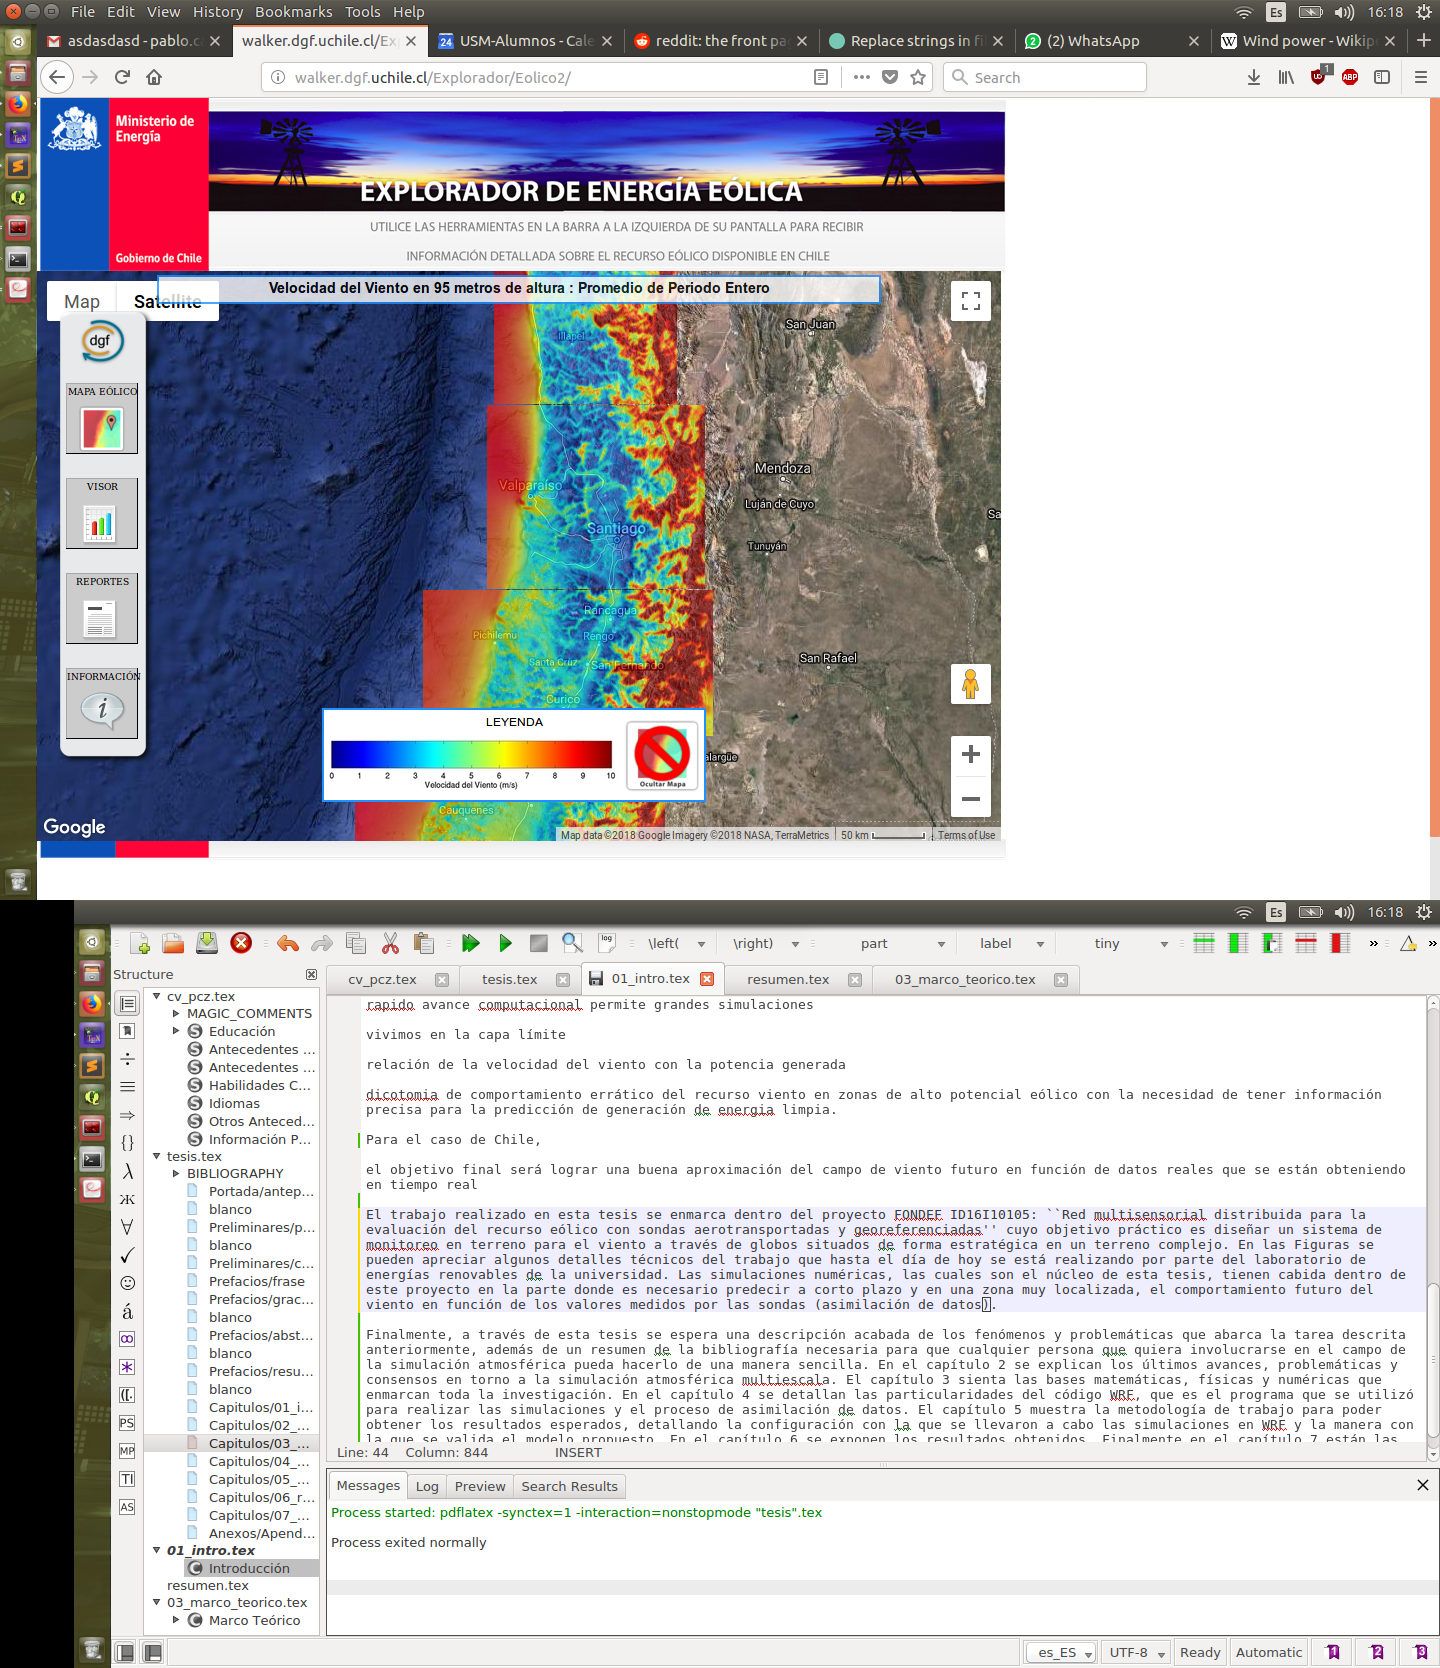
\includegraphics[width=0.9\linewidth,trim={1.4cm 28cm 15cm 3.4cm},clip]{Imagenes/01/explo}
	\caption{Interfaz online del explorador eólico de la Universidad de Chile.}
	\label{fig:01_explorador}
\end{figure}

Localmente en Chile cada año se están inaugurando nuevos parques eólicos debido al buen factor de planta que se poseen en ciertas zonas del país \citep{anuariocne2018}. Hasta la fecha ya se han instalado mas de 600 turbinas eólicas y la tendencia es a que este número siga aumentando. Actualmente Chile posee una potencia instalada de $23.315$ [MW], de los cuales un 7\% corresponde a energía eólica \citep{anuariocne2018}. El año 2017 se tenía un 6\% y el 2008 era menor a 1\%. De la mano de la instalación de nuevas plantas, está la simulación numérica realizada para tener una estimación de la cantidad de energía que se puede llegar a generar. En el 2010, la Universidad de Chile entregó a la comunidad la herramienta online llamada Explorador Eólico, en esta se muestra el potencial eólico que tiene gran parte de Chile, el cual fue simulado utilizando el modelo WRF. Algunos resultados de esta herramienta se pueden ver en la Figura \ref{fig:01_explorador}.

Si bien esta herramienta ha entregado a la comunidad información certera y que antes no existía, las simulaciones realizadas para el Explorador Eólico contemplaban mallas numéricas con una resolución horizontal máxima de 1 [km], lo que no es suficiente para resolver el comportamiento turbulento de microescala, ni para captar efectivamente las variaciones orográficas muy importantes para energía eólica. El comportamiento del viento a lo largo de una superficie de 1 [km$^2$] puede cambiar mucho, en especial si existe terreno complejo, y por lo tanto la ubicación o no de una turbina eólica requiere un análisis mas detallado del dominio.

El objetivo es entonces buscar una buena aproximación para el campo de viento en la capa límite en terrenos complejos y a alta resolución, a modo de tener una evaluación mas realista para la toma de decisiones en situaciones en donde el viento sea una variable crítica.

Debido a que en la capa límite es donde predominan los fenómenos de mezcla y turbulencia, es acá en donde los modelos presentan la mayoría de sus problemas operativos y desviaciones, y de hecho, el buen comportamiento del un modelo va a depender en gran manera de la habilidad del \emph{solver} para ajustar ciertos parámetros arbitrarios del código. 

Dado que la filosofía de este trabajo es utilizar la información original sin ser manipulada y evitar el ajuste de parámetros, es que se busca la manera de corregir los resultados numéricos a través de un proceso de asimilación de datos utilizando los valores paramétricos medidos en terreno.

La asimilación de datos es el proceso matemático mediante el cual se combina información de observaciones y de simulación numérica para obtener la mejor estimación del estado real de la atmósfera en un instante dado. Este proceso se utiliza cotidianamente en modelos globales o sinópticos para entregar la información sobre el clima que se presenta día a día en los noticieros.

Para los modelos meteorológicos mesoescala, el realizar asimilación de datos en la microescala no presenta beneficios, debido a que generalmente la resolución de estos modelos es gruesa en las cercanías de la superficie (la capa límite está pobremente resuelta), lo que se traduce en que la combinación entre observaciones superficiales y resultados numéricos no es fiable.

Sin embargo, y considerando esto como motivación para esta investigación, si se trabaja a resoluciones lo suficientemente altas como para tener información confiable en las cercanías de la superficie, si es posible realizar asimilación de datos en la microescala y por lo tanto mejorar los pronósticos del viento en la capa de superficie.

El trabajo realizado en esta tesis se enmarca dentro del proyecto FONDEF ID16I10105: ``Red multisensorial distribuida para la evaluación del recurso eólico con sondas aerotransportadas y georeferenciadas'' cuyo objetivo práctico es diseñar una red neuronal para monitoreo del viento a través de globos situados de forma estratégica en un terreno complejo. Dicha red de sondas cautivas constituye un sistema de acopio de datos multiparamétricos que alimentarán un modelo numérico como WRF. En las Figuras \ref{fig:01_detalle_fondef} y \ref{fig:01_sonda} se pueden apreciar algunos detalles técnicos del trabajo que hasta el día de hoy se está realizando por parte del Laboratorio de Energías Renovables de la UTFSM. Las simulaciones numéricas, las cuales son el núcleo de esta tesis, tienen cabida dentro de este proyecto en la parte donde es necesario predecir a corto plazo y en una zona muy localizada, el comportamiento futuro del viento en función de los valores medidos por las sondas (proceso de asimilación de datos).

\begin{figure}
	\begin{minipage}{0.5\linewidth}
		\centering
		(a)
	\end{minipage}
	\begin{minipage}{0.5\linewidth}
		\centering
		(b)
	\end{minipage}
	
	\begin{minipage}{0.5\linewidth}
		\centering
		\includegraphics[width=0.9\linewidth,page=3,trim={6cm 12.2cm 6cm 9.5cm},clip]{Imagenes/01/descrp}
	\end{minipage}
	\begin{minipage}{0.5\linewidth}
		\centering
		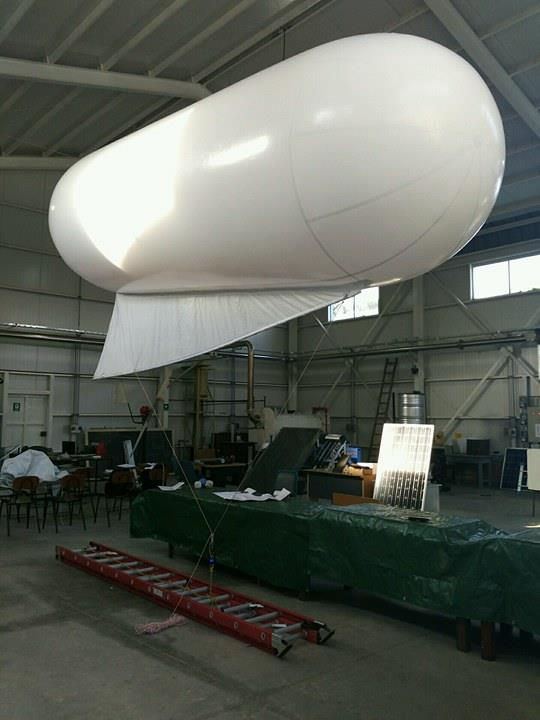
\includegraphics[width=0.7\linewidth,trim={0cm 0cm 0cm 0cm},clip]{Imagenes/01/prototipo}
	\end{minipage}
	\caption{Detalle del proyecto FONDEF ID16I10105. (a) Célula del sistema experimental de medición. (b) Prototipo en el laboratorio.}
	\label{fig:01_detalle_fondef}
\end{figure}

El objetivo final de esta investigación es implementar un sistema robusto que obtenga una buena aproximación del campo de viento futuro en función del ajuste pronóstico  datos medidos que se obtienen en tiempo real, mediante simulaciones numéricas multiescala realizadas con el software libre WRF y asimilación de datos 4D. La filosofía de simulación, será realizarlas de la manera menos manipulada posible, utilizando bases de datos públicas y evitando la asignación arbitraria de parámetros. Este enfoque ha sido poco investigado para la predicción y caracterización eólica en terreno real a alta resolución. 

\begin{figure}[h!]
	\centering
	\includegraphics[width=0.82\linewidth,page=5,trim={3cm 2cm 2.3cm 3cm},clip]{Imagenes/01/descrp}
	\caption{Esquema de la sonda FONDEF ID16I10105.}
	\label{fig:01_sonda}
\end{figure}

En el presente trabajo se brinda una descripción acabada de los fenómenos y problemáticas que abarca la tarea descrita anteriormente, además de un resumen de la bibliografía necesaria para que cualquier persona que quiera involucrarse en el campo de la simulación atmosférica con asimilación de datos pueda hacerlo de una manera sencilla. Como beneficio para la comunidad científica, los resultados obtenidos podrán ser utilizados como linea de base (o benchmark) para cualquier otra simulación futura a alta resolución, pudiendo dar pie a una nueva prueba canónica para modelos multiescala en operación continua.

\section{Hipótesis}
A través de simulaciones numéricas multiescala de alta resolución con un modelo atmosférico y un esquema de asimilación de datos 4D dentro de la capa límite planetaria, es posible obtener un pronóstico preciso a corto plazo para viento sobre terreno complejo y representar correctamente el comportamiento turbulento de este.

\section{Objetivos}
\subsubsection{Objetivo Principal}
\begin{itemize*}
	\item Mejorar la precisión de los pronósticos de la capa límite planetaria a través de simulaciones atmosféricas multiescala de alta resolución sobre terreno complejo con la incorporación de un esquema de asimilación de datos 4D multipunto para alimentar datos al sistema en tiempo real y lograr un ajuste adecuado de las variables.
	%\item Lograr a través de la aplicación de asimilación de datos 4D multipunto en la capa límite atmosférica una mejora comparativa con respecto a los modelos existentes para la predicción de viento a alta resolución en terreno complejo en el modelo de código libre WRF.
\end{itemize*}
\subsubsection{Objetivos Secundarios}
\begin{itemize*}
	\item Acoplar dominios de microescala y mesoescala en simulaciones numéricas atmosféricas para el uso eficiente del esquema de clausura turbulenta tipo LES.
	\item Estudiar e incorporar una metodología para usar bases de datos reales de alta resolución para orografía y uso de suelo en el modelo WRF.
	\item Desarrollar y optimizar el método y código para la simulación atmosférica multiescala y asimilación de datos.
	\item Estudiar la influencia de la asimilación de datos en la simulación computacional de la capa límite considerando un solo punto y múltiples puntos (estaciones) de monitoreo.
	\item Verificar y validar resultados obtenidos con aquellos estudios publicados en la literatura y basados en campañas de medición en terrenos reales.
	\item Generar una base de datos de resultados para terreno complejo real utilizable como base de comparación y validación para la comunidad científica. 
\end{itemize*}
\newpage
\section{Estructura del Documento}
La estructura de esta tesis se organiza de la siguiente manera:
\begin{itemize*}
	\item Cap. 2: Se exponen los últimos avances, problemáticas y tendencias en torno a la simulación atmosférica multiescala y asimilación de datos, que son el núcleo del trabajo realizado.
	\item Cap. 3: Sienta las bases conceptuales, matemáticas y físicas sobre las cuales se desarrolla la investigación. Se abordan: las leyes fundamentales de los fluidos, la dinámica atmosférica, la turbulencia, la capa límite planetaria, el método de simulación de grandes vórtices (LES) y la asimilación de datos 4D.
	\item Cap. 4: Se explica el funcionamiento del software  libre WRF y la metodología implementada para este estudio.
	\item Cap. 5: Muestra la filosofía y configuración de los 4 experimentos realizados: 2 casos para terreno plano (donde uno sirve como validación y el otro analiza la asimilación de datos) y dos casos para terreno complejo (sin y con asimilación). Además, se detalla la metodología para la obtención, postprocesamiento y presentación de resultados.
	\item Cap. 6: Se presentan y analizan detalladamente los resultados mas relevantes.
	\item Cap. 7: Conclusiones, trabajo futuro y propuestas de mejora para el trabajo/método implementado.
\end{itemize*}

%
\chapter{Estado del Arte}
Tomando en consideración lo amplio, en el sentido de las disciplinas a abarcar, de este trabajo de tesis, el resumen del estado del arte para este se llevará a cabo en cuatro secciones distintas. 

Primero se expondrá la problemática que nace debido a la turbulencia en las simulaciones multiescala. Luego se revisará la historia y la creciente utilización de la técnica de Simulación de Grandes Vórtices (de aquí en adelante \emph{Large Eddy Simulation} o LES) en la solución numérica de los modelos meteorológicos. Tercero, se verán las complicaciones y los desafíos que conlleva el realizar simulaciones de alta resolución en terreno complejo y los consensos internacionales tomados al respecto. Finalmente se mostrará el estado actual de la utilización de los métodos de asimilación de datos para el uso operacional en el contexto de las simulaciones atmosféricas y en la capa límite.
\section{Simulación Multiescala y Zona Gris}
Como ya se justificó en la introducción, la predicción atmosférica en zonas localizadas, en especial en aquellas con terreno irregular, es un tema de especial relevancia en las áreas del cambio climático, la contaminación ambiental y la industria energética. Actualmente las simulaciones climáticas regionales se realizan con una resolución de malla del orden de los kilómetros. Esto es, evidentemente, insuficiente para poder representar fehacientemente cualquier topografía compleja, y por lo tanto, insuficiente también para resolver los fenómenos meteorológicos asociados a esta.

Una manera de solucionar esto puede ser el eso de un escalamiento estadístico para llevar las soluciones a una malla mas fina, sin embargo, este acercamiento no contempla ni la física fundamental ni las no-linealidades, que son la característica mas importante del comportamiento de la atmósfera en su interacción con el terreno complejo. Su contraparte, el escalamiento dinámico, permite anidar mallas y resolver las leyes de conservación para resoluciones cada vez mas altas hasta lo que se desee resolver, teniendo como limitantes: el costo computacional, la precisión de las condiciones de borde y las parametrizaciones físicas que se incorporarán a las ecuaciones. Para este trabajo, es claro el beneficio que trae el utilizar el escalamiento dinámico como metodología para alcanzar simulaciones de alta resolución y por lo tanto ese es el acercamiento que se utilizará.

A modo de formar una explicación un poco mas formal y clara sobre lo que conlleva el realizar una simulación atmosférica multiescala, tomemos en consideración la Figura \ref{fig:02_escalas} para identificar las distintas escalas temporales y espaciales.

\begin{figure}[h!]
	\centering
	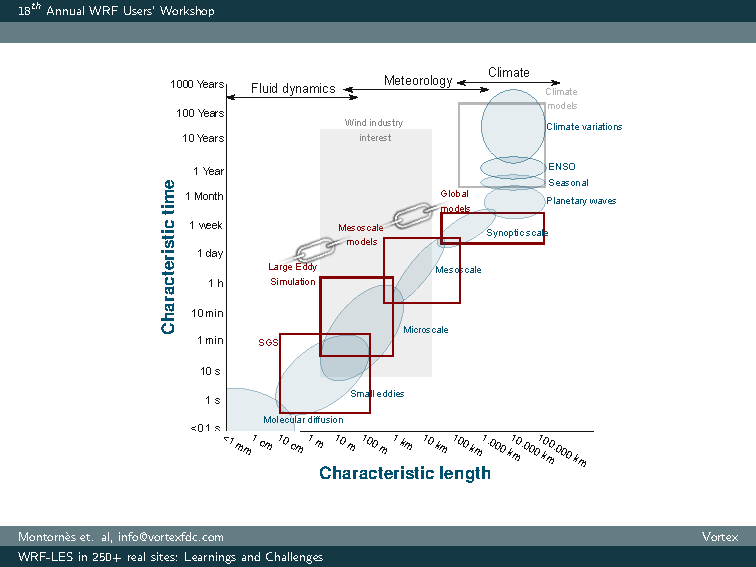
\includegraphics[width=0.85\linewidth,trim={2.6cm 1.4cm 1.5cm 0.8cm},clip]{Imagenes/02/escalas}
	\caption{Separación de escalas para la dinámica atmosférica.}
	\label{fig:02_escalas}
\end{figure}

La figura en cuestión muestra tres aspectos claves de las simulaciones atmosféricas que se desean realizar: las áreas del conocimiento involucradas, los fenómenos que resuelve cada área y las escalas asociadas a cada uno de estas.

Nos referimos a simulación multiescala cuando, a través de algún proceso de escalamiento y simulación numérica se resuelven simultáneamente distintas escalas espaciales y se representan correctamente sus fenómenos asociados.
 
Nos referimos, por otra parte, a escalamiento dinámico, cuando se resuelven escalas mas pequeñas usando como base una escala mas grande, la cual es usada como condición inicial y de contorno en un subdominio de un dominio general. De esta forma es posible tener resultados numéricos para la microescala partiendo desde una escala, por ejemplo, global. 

En el contexto del trabajo a realizar, las escalas temporales pertenecientes a las simulaciones serán del orden de los días, por lo tanto, los fenómenos que se engloban dentro de estas son una combinación entre fenómenos de microescala, mesoescala y escala sinóptica. El buen comportamiento del resultado de una simulación estará directamente relacionado con lo bien representado que estén cada uno de estos fenómenos dentro del modelo.

De manera general, el escalamiento dinámico funciona bien y solo incorpora al modelo un error de interpolación debido al traspaso de una malla mas gruesa a otra mas fina. Sin embargo, la presencia de la turbulencia a lo largo de todo el espectro de escalas complica el escalamiento desde la mesoescala hasta la microescala.

Para entender la complejidad asociada a la presencia de la turbulencia debido al escalamiento dinámico, hay que entender primero la manera en la que actúan las distintas fuerzas que controlan el movimiento atmosférico. Si se considera, por ejemplo, la fuerza de Coriolis que es el motor principal de los ciclones y anticiclones en los hemisferios, esta fuerza es relevante en escalas sinópticas y globales y si se quisiera resolver ecuaciones a un nivel de mesoescala, podrían ser válidamente despreciadas. Por otra parte, si se considera ahora, la disipación viscosa generada por el roce entre los distintos elementos diferenciales de aire, esta podría ser válidamente despreciada también en todas las escalas debido a que la viscosidad del aire es muy baja, sin embargo si se desea analizar la parte viscosa de la capa límite atmosférica, este término es fundamental y no podría despreciarse\footnote{Un análisis mas detallado de las distintas fuerzas existentes dentro de las ecuaciones que modelan el comportamiento atmosférico y su correspondiente análisis en órdenes de magnitud se dará en el próximo capítulo.}. 
 
Se concluye entonces que las distintas fuerzas que aparecen en las ecuaciones tienen un cierto rango de escalas propias donde contribuyen fuertemente al movimiento atmosférico. 

La turbulencia sin embargo\footnote{Probablemente le haga ruido al lector el hecho que hasta ahora no se ha presentado una definición formal de la turbulencia. Como esta requiere una descripción matemática extensa se prefirió dejarla para el próximo capítulo.}, no funciona de la misma forma. Los vórtices de distintos tamaños que habitan en la atmósfera son igualmente importantes en términos de órdenes de magnitud para las ecuaciones que se resuelven.

Cuando se modelan las grandes escalas (sinóptica, mesoescala), generalmente la resolución de malla horizontal es demasiado grande como para captar los vórtices y por lo tanto el efecto de estos en las ecuaciones queda filtrado numéricamente. Operacionalmente, esta operación de filtrado se revierte con la utilización de un esquema adecuado para parametrizar la turbulencia. En los modelos meteorológicos actuales este efecto generalmente queda confinado en la llamada \emph{parametrización de capa límite}, ya que el principal rol que cumple la turbulencia en estas escalas es la de transmitir la información que se genera a nivel de superficie terrestre a la atmósfera libre.

Cuando se modelan las pequeñas escalas, idealmente la resolución de malla horizontal va a bastar para captar de manera adecuada cierto espectro de los vórtices generados por el efecto de la turbulencia y por lo tanto se puede omitir la parametrización de capa límite. Es importante notar que si bien ahora se resuelven los vórtices grandes que provocan la mezcla dentro de la capa límite, otra parte de los vórtices sigue sin ser resuelta\footnote{Esto debido a que la cascada de energía turbulenta existe hasta el órden de los milímetros.} y por lo tanto se deberá utilizar otro modelo turbulento para modelarla. Esta modelación será la encargada de representar la cascada de energía y la disipación de energía turbulenta.

\begin{figure}[h!]
	\centering
	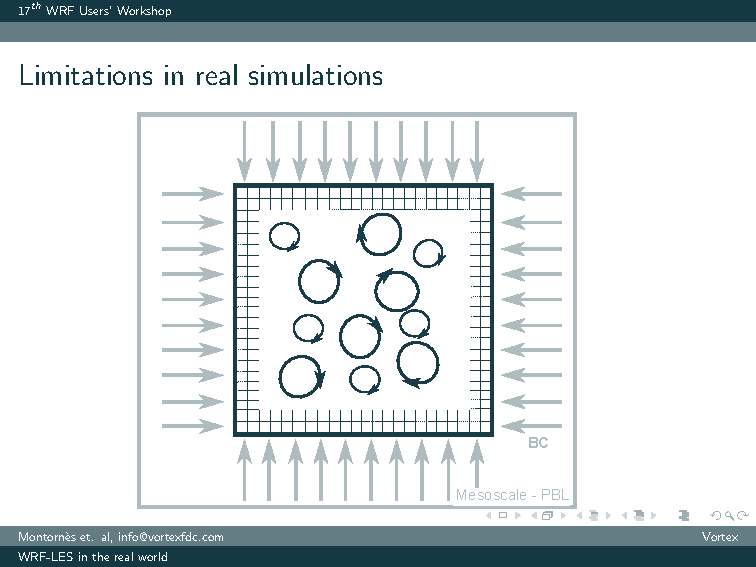
\includegraphics[width=0.5\linewidth,trim={2.67cm 1.35cm 3.1cm 2.25cm},clip]{Imagenes/02/grid}
	\caption{Idealización de los distintos tamaños de vórtices dentro de un dominio en la zona gris de la turbulencia. Los vórtices mas grandes pueden ser resueltos por la malla, mientras que los más pequeños son filtrados numéricamente y por lo tanto deben ser parametrizados para que su efecto se considere en las ecuaciones de movimiento.}
	\label{fig:02_grid_vortex}
\end{figure}

Reflexionando un poco con respecto al rol que toma la turbulencia tanto en las escalas grandes como en las pequeñas, no es difícil llegar a la conclusión que a través del proceso de escalamiento dinámico se llegará eventualmente a una zona de traslape en donde algunos de los vórtices asociados a la capa límite son indistintamente resueltos y modelados. La Figura \ref{fig:02_grid_vortex} representa este hecho. 

A esta zona de traslape se le denomina zona gris o \emph{Terra Incognita}.

Utilizando la terminología de Wyngaard (2004), sea $\Delta$ la escala (o tamaño) del filtro espacial asociado a la solución numérica (o malla) de las ecuaciones de movimiento y $l$ la escala característica de los vórtices en el rango inercial, el espectro de energía turbulenta $\phi(\lambda)$ se ve como se muestra en la Figura \ref{fig:02_terra_inc}.

\begin{figure}[H]
	\centering
	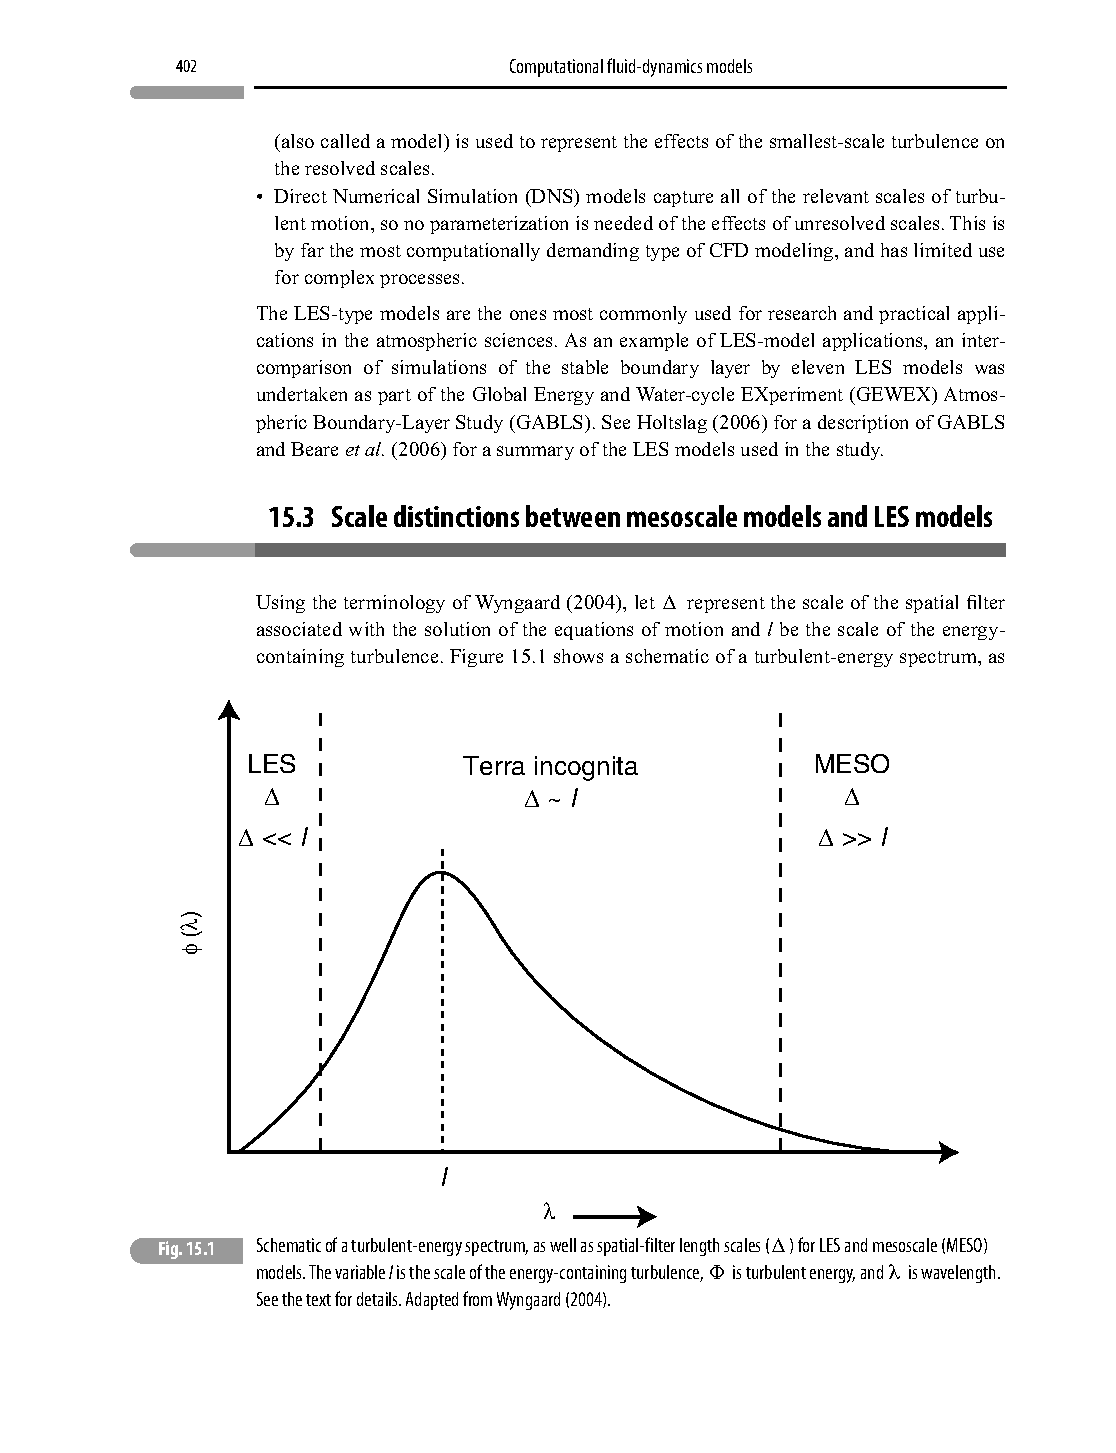
\includegraphics[width=0.8\linewidth,trim={2cm 3.0cm 1.5cm 11.5cm},clip]{Imagenes/02/terra_inc}
	\caption{Espectro de energía turbulenta multiescala.}
	\label{fig:02_terra_inc}
\end{figure}

Para valores de $\Delta\gg l$ asociados a la mesoescala, la producción de energía turbulenta queda por debajo del filtro y por lo tanto, tiene sentido que se modele a través de un esquema de submalla. Por otro lado, para valores de $\Delta\ll l$ los vórtices que contienen la energía pueden ser completamente modelado por las ecuaciones y entonces no debe usarse un SGS (microescala).

Queda entonces el rango en donde $\Delta\sim l$. Dentro de este intervalo se desconoce cual es el comportamiento de los modelos atmosféricos ya que existe una doble representación de tanto los vórtices que se resuelven como los que se modelan.

En la práctica, el acercamiento para compensar este problema es definir los dominios de modo que se evite usar el modelo en el rango de la \emph{Terra Incognita}.
\section{Turbulencia Atmosférica y LES}
Tomando como antecedente la problemática que induce la turbulencia al intentar solucionar numéricamente las ecuaciones que rigen el comportamiento atmosférico utilizando un enfoque multiescala, en esta sección se describirá brevemente la historia del tratamiento especial que tiene la turbulencia, se introducirá el modelo LES para representar los esfuerzos de submalla y los principales avances en los últimos años.

Los primeros modelos desarrollados para poder estimar el potencial eólico parten en el año 1975, donde Jackson y Hunt presentan su análisis bidimensional para flujo turbulento en terreno complejo, el cual en 1979 fue ampliado a 3D por Mason y Stykes. Estos modelos tienen la particularidad de ser lineales y el beneficio de presentar resultados computacionalmente rápidos para pendientes no mayores a 17$^\circ$. Estos mismos modelos lineales, mejorados, actualmente se utilizan en códigos comerciales como MS3DJH, MSFD y WAsP.

En forma paralela a los modelos lineales, se fueron desarrollando métodos numéricos para resolver las ecuaciones no lineales. En 1977 Taylor desarrollo un modelo 2D no lineal de diferencias finitas para el flujo sobre una colina pequeña. Entre el 1970 y 1980 el desarrollo de algoritmos para solucionar las ecuaciones RANS fue intensivo y esto resultó en el origen de una gama de modelos de clausura para la turbulencia. El modelo clásico $k-\epsilon$ fue originalmente propuesto en 1974 por Launder y Spalding y entre los años 80s y 90s se formularon varias modificaciones para flujos atmosféricos. En este punto, los modelos RANS presentaban una mejor solución en términos de la aceleración en la cima de las colinas y el comportamiento aguas abajo de estas.

Luego, desde los años 90s, la técnica de simulación de grandes vórtices (LES) se ha estado aplicando a la capa límite planetaria sobre terreno plano homogéneo. El argumento a favor de la utilización del LES es que con el incremento de la potencia computacional y el refinamiento de las mallas, eventualmente se debería llegar a soluciones que sean independientes del modelo de clausura para la turbulencia. Si bien esto es teóricamente correcto, el terreno real posee rugosidad y por lo tanto se requieren modelos de pared avanzados. Estos modelos aún son dependientes del tipo de parametrización que se escoja en el método numérico.

Las simulaciones LES en terreno real entonces, se ven enfrentadas a, por lo menos, dos grandes problemas: el elevado costo computacional asociado a los tamaños de malla y el acoplamiento entre la cercanía de la pared, altamente parametrizada, con la región exterior resuelta.

A pesar de los desafíos que debe superar el LES, su potencial para modelar flujos a través de colinas ha sido altamente reconocido. Diversos autores han modelado correctamente el campo de viento en la colina Askeverin (Chow y Street, 2009; Bechmann y Sørensen 2010b) y cerros sinusoidales (Brown et al. 2001; Wan et. al. 2007), sin embargo pocos estudios en terreno complejo real existen.
\section{Alta Resolución y Terreno Complejo}
Como motivación, se comienza esta sección haciendo una pequeña derivación de la importancia de una correcta estimación de la velocidad del viento. Luego se expondrán los consensos tomados el año 2012 por el \emph{HiRCoT Workshop} (High Resolution Modelling in Complex Terrain), los cuales resumen de muy buena forma las bases y desafios actuales sobre este tema particular y que tienen especial importancia en el trabajo a desarrollar.
\subsection{Importancia de la Estimación del Viento}
Para tener un acercamiento a la importancia de la correcta estimación del viento, consideremos la energía cinética del viento. Para un área arbitraria de magnitud $A$ en un tiempo $t$ se tiene:
\begin{equation} 
E_k = \frac{1}{2}mV^2 = \frac{1}{2}(AVt\rho)V^2 = \frac{1}{2}At\rho V^3
\end{equation}

Donde $\rho$ es la densidad del aire y $V$ es la rapidez del viento. $AVt$ es entonces el volumen de aire pasando por el área $A$ que se define como normal a la dirección de la velocidad del viento $V$. La potencia del viento (energía por unidad de tiempo) para el caso de una turbina eólica queda definida entonces como:
\begin{equation}
P = \frac{E_k}{t} = \frac{1}{2}A\rho V^3
\end{equation}

Donde $A$ pasa a ser ahora el área del rotor de la turbina. La potencia del viento, es entonces, proporcional al cubo de la velocidad del viento.

Se puede derivar la ecuación anterior para hallar una relación entre los errores relativos de las dos variables de interés. Derivando la ecuación anterior se obtiene:

\begin{equation}
dP = \frac{1}{2}A\rho\cdot d(V^3) = \frac{3}{2}A\rho V^2 dV
\end{equation}

Y dividiendo ahora por la potencia eólica:
\begin{equation}
\frac{dP}{P} = 3\frac{dV}{V}
\end{equation}

Lo que significa que un error relativo (o porcentual) en una estimación de la velocidad del viento, conlleva a un error el triple mas grande para la potencia que se podría generar.

Anteriormente ya se había hablado de la relación que existe entre la complejidad del terreno y la velocidad del viento. Los fenómenos asociados a la orografía y las no linealidades provocan que la predicción del viento en estas zonas sea especialmente difícil. 

Como consecuencia, es de especial interés analizar las problemáticas que induce el terreno complejo y definir las maneras de como abordarlas.
\subsection{Problemáticas de la Simulación de Alta Resolución}
El año 2012 se llevo a cabo en Viena, el primer \emph{HiRCoT Workshop}, instancia que reunió a académicos y personas de la industria a debatir activamente sobre las problemáticas y avances existentes con respecto a la modelación atmosférica a alta resolución \cite{Arnold2010}.

El concepto de alta resolución, se debe entender en el sentido de una resolución que está por sobre aquella definida por los desarrolladores para utilizar los modelos. A priori se podría decir que un modelo atmosférico con una resolución de malla menor a 1 [km] entra en esta categoría.

Dentro de los objetivos específicos definidos en este workshop se incluyen: la identificación de problemas asociados a la simulación numérica en terreno complejo y el mapeo de las posibilidades de como manejar estos, por lo tanto las conclusiones emanadas de ese taller sirven como buenos cimientos para este trabajo de tesis.

A continuación se presenta un resumen de los cuatro aspectos estudiados en el workshop y que se deben tener en consideración a la hora de realizar una simulación atmosférica a alta resolución y para la lectura de esta tesis.

\subsubsection{Aspecto 1: Problemas Computacionales}
Tomando en consideración que existen casos demostrados en donde la alta resolución es una necesidad para simular realísticamente fenómenos meteorológicos asociados a las escalas sinópticas y mesoescala, queda claro que, para desarrollar simulaciones a alta resolución en terreno complejo, se debe asumir un cierto compromiso computacional. El wokrshop identifica 2 temas principales: los relacionados a los tiempos de simulación y aquellos relacionados al rendimiento I/O del código.

Con respecto al tiempo de simulación, se abordó el tema de como impacta en este el hecho de llevar una simulación con resolución de 9 [km] a 1 [km]. Si se mantienen los límites de los dominios numéricos constantes, el aumento en la resolución de la malla traerá consigo un aumento de la cantidad de puntos necesarios para simular. Por otro lado, este refinamiento también exigirá un paso de tiempo menor para evitar la violación de la condición CFL. En el mejor de los casos entonces, pasar de una resolución de 9 [km] a 1 [km] en la cual la primera se demore, por ejemplo, 1 hora, implicará que la simulación a alta resolución se va a demorar aproximadamente 1 mes. Actualmente no existen maneras de reducir este aumento considerable en los tiempos de cálculo y por lo tanto pasa mas a ser un limitante en el diseño experimental. Pequeñas mejoras se pueden obtener si se adopta el uso de un paso de tiempo adaptativo, pero esto puede crear incongruencias en los tiempos de obtención de resultados del modelo, en especial para la aplicación de asimilación de datos. La paralelización de procesos también puede ayudar bastante, sin embargo para el análisis de este caso, ambas simulaciones estuvieron masivamente paralelizadas.

Con respecto al rendimiento en I/O, y que tiene especial relación con lo descrito en el párrafo anterior, el aumento en la cantidad de puntos de malla, y la disminución en el paso de tiempo, significa un aumento considerable en término de memoria para cada uno de los procesos con los que se ejecuta el código. En la arquitectura del WRF (y en la mayoría de los modelos atmosféricos) el cálculo se paraleliza en tantos procesos como procesadores se disponga utilizando un paradigma de maestro/esclavo en donde un único proceso maestro es el encargado de ejecutar las funciones de entrada/salida del modelo. A grandes rasgos el aumento de los puntos de malla no afecta tanto a los procesos que son esclavos, pero el proceso maestro si sufre de un cuello de botella al ser el encargado de leer y ubicar todas las variables globales a cada proceso. Como ejemplo académico, consideremos un dominio de 448 millones de puntos ($4000\times4000\times28$) en un servidor con 75 nodos de 4 núcleos cada uno. En este ejemplo cada proceso usará un total de 1.9GBytes, sin embargo el proceso maestro requerirá un extra de 1.8GBytes para las funciones de I/O, pudiendo ser un potencial punto de falla. En la actualidad se estan desarrollando nuevos formatos y paradigmas para facilitar la paralelización de este tipo de tareas, sin embargo una implementación de estos no se ve en el corto plazo.

\subsubsection{Aspecto 2: Problemas Numéricos}
Corresponden a las problemáticas asociadas a la discretización por la implementación de los esquemas numéricos para resolver las ecuaciones que rigen el comportamiento atmosférico. Se identificaron 5 grandes grupos:
\begin{itemize*}
	\item Precisión
	\item Estabilidad
	\item Difusión numérica (explícita e implícita)
	\item Coordenadas
	\item Necesidad de Benchmark
\end{itemize*}

El éxito de una simulación a alta resolución dependerá fuertemente del conocimiento de los aspectos técnicos relacionados a uso de los esquemas numéricos en el modelo a usar. Como base, la gran mayoría de los modelos atmosféricos utiliza un esquema de diferencias finitas y la integración temporal se hace de manera explícita. Esta selección en el modo de integrar numéricamente limita en gran medida la estabilidad del esquema ya que no se debe violar la condición CFL. La implementación de un esquema implícito permite ganar estabilidad, en el sentido de la condición CFL, sin embargo las numéricas se complejizan y la resolución implica ahora solucionar una ecuación elíptica la cual es difícil de paralelizar en super computadores.

La presencia de terreno complejo por otra parte, incentiva la aparición de ruido numérico debido al desarrollo de perturbaciones de alta frecuencia las cuales desafían la precisión del esquema de advección, los gradientes de presión y la consistencia de los términos métricos. Para evitar esto se suele suavizar el terreno, aunque para el caso de una simulación a alta resolución esto no es deseable ya que se pierde una parte sustancial de la fineza del terreno, que es lo que se quería ganar en primer lugar. 

\paragraph{Precisión} Se entiende como precisión, el orden con el cual se reducen los errores de truncación debido a un refinamiento temporal o espacial. Mejores esquemas numéricos implican una mejor precisión, sin embargo son mas costosos computacionalmente. Para simulaciones a alta resolución en terreno complejo, los datos utilizados para inicializar el modelo ya vienen con una resolución propia de los instrumentos de medición usados. Estos datos pueden ensuciar la precisión formal que tenga un cierto esquema numérico debido a que los errores inducidos por los datos predominaran por sobre aquellos del modelo. De ahí que para este tipo de simulaciones, la utilización de esquemas de alto orden no se presenta como un beneficio tan tangible.

\paragraph{Estabilidad} Como se habló anteriormente, debido a la predominancia de los esquemas explícitos, los modelos de NWP están sujetos a criterios de estabilidad numérica. El primer criterio es el CFL, asociado a la advección, donde se debe cumplir que:
\begin{equation}\label{eq:cfl}
\frac{c\Delta t}{\Delta x}<\beta_a
\end{equation}
Donde $c$ es es la rapidez de propagación física de una señal y $\beta_a$ es un coeficiente que depende de la discretización. El otro criterio importante es el asociado a la difusión, el cual se escribe como:
\begin{equation}\label{eq:cfl_d}
\frac{M\Delta t}{\Delta x^2}<\beta_d
\end{equation}
Acá $M$ es un coeficiente de difusión y $\beta_d$ es otro coeficiente que depende de la discretización. Notar que en este segundo criterio, el valor escala de manera cuadrática con $\Delta x$, lo que implica que $\Delta t$ deberá disminuir proporcionalmente a $\Delta x^2$ para mantener estable la integración de los términos difusivos. En simulaciones estándar, el común usar un coeficiente de difusión que escale según $\Delta x^2$ (Smagorinsky por ejemplo), luego este criterio es mas vulnerable a ser violado a muy alta resolución.

Algunas técnicas prácticas que se utilizan para evitar las inestabilidades incluyen el uso de pasos de tiempo adaptativos que impidan el no cumplimiento de los criterios antes mencionados o el uso de amortiguamiento para la componente $w$ de la velocidad, que es la mas crítica en la simulación de terreno complejo. El uso de amortiguamiento genera soluciones no físicas y por lo tanto no está bien visto por la comunidad científica.

\paragraph{Difusión Numérica} La difusión artificial (o numérica) o disipación artificial es la amortiguación sucesiva de perturbaciones como consecuencia de las propiedades del método numérico. De la misma manera en la que actúa la difusión física, las variaciones de las escalas pequeñas se tienden a suavizar. Esto puede ser provocado implícitamente debido a la diferenciación espacial o explícitamente como un término en las ecuaciones resueltas. Este es un fenómeno complejo y generalmente el manejo de este se encarga a los diseñadores de los núcleos dinámicos de los modelos. A nivel de usuario, una regla práctica es saber que aquellos esquemas espaciales que son de orden par poseen una mayor difusión que aquellos de orden impar, por ende se prefiere el uso de estos últimos.

La difusión artificial posee algunos aspectos positivos, puede mantener bajo control el ruido numérico que se provoca a pequeñas escalas, sin embargo, si existe mucha difusión numérica toda una simulación realizada a alta resolución puede verse suavizada debido al efecto de esta y podría no rescatarse el comportamiento debido al terreno complejo.

Para ámbitos operativos, se prefiere no utilizar difusión horizontal explícita o realizarla solo en coordenadas reales. La difusión implicita es mas dificil de controlar, pero esta no afecta de gran manera al comportamiento sobre terreno complejo a no ser para grandes magnitudes del viento. 
\paragraph{Coordenadas} Para solucionar las ecuaciones que gobiernan el comportamiento atmosférico, los modelos NWP utilizan sistemas coordenados no necesariamente Cartesianos. La mayoría de los modelos utiliza sistemas que persiguen la forma del terreno, entre los que se pueden nombrar:
\begin{itemize*}
	\item Coordenadas ``sigma'' de presión o coordenadas de altura.
	\item Coordenadas curvilíneas adaptadas al borde.
	\item Coordenadas Cartesianas con el método de frontera inmersa.
\end{itemize*}

 
\begin{figure}[h!]
	\centering
	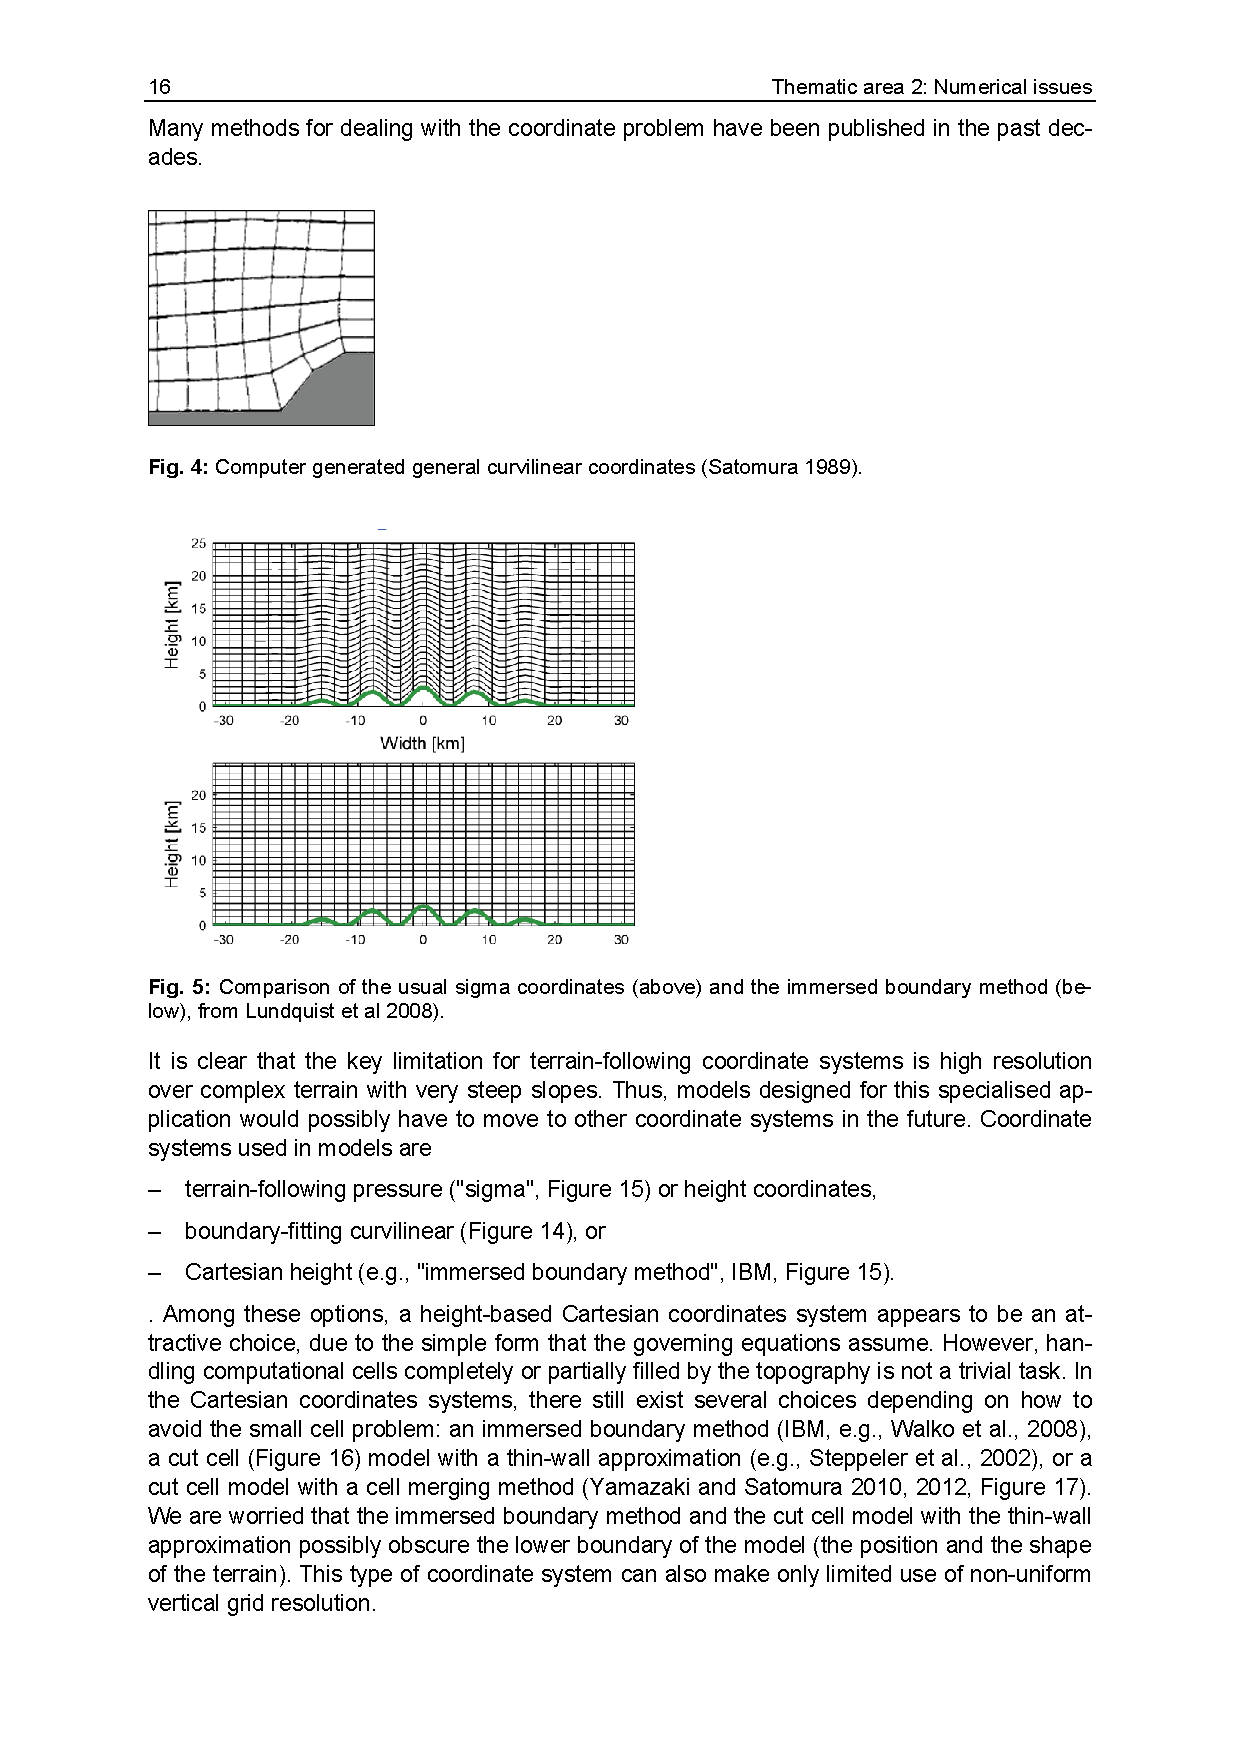
\includegraphics[width=0.8\linewidth,trim={2.6cm 13.5cm 9.2cm 9cm},clip]{Imagenes/02/coordinates}
	\caption{Comparación entre las coordenadas usuales sigma (arriba) y el método de frontera inmersa (abajo).}
	\label{fig:02_coordinates}
\end{figure}
La transformación de coordenadas naturales a curvilíneas provoca en las ecuaciones gobernantes la aparición de términos métricos, los cuales son difíciles de manejar en pendientes abruptas, pero permite captar bien la forma del terreno. Por otra parte el uso del método de la frontera inmersa no incluye cambio en las ecuaciones pero en manejo de las celdas que están parcialmente ocupadas por orografía no es una tarea computacional sencilla.

Si bien, para cualquiera de estos dos casos existen problemáticas computacionales que no son fáciles de solucionar, la mas limitante en la actualidad es el manejo de las pendientes abruptas y la exigencia que esto significa en la resolución de malla vertical y la aritmética de grandes diferencias de presión. Por lo tanto, el pronóstico de la comunidad, es a migrar a un sistema coordenado cartesiano utilizando el método de frontera inmersa u otros métodos similares en la cercanía del terreno, como la aproximación de pared delgada (Steppeler et. al., 2002) o el método de unión de celdas (Yamazaki y Satomura 2010,2012).

\paragraph{Benchmarking} La existencia de benchmarks (casos de comparación) es clave para este tipo de simulaciones. Lo que se posee actualmente son casos ideales de colinas gausianas para el estudio de ondas de montañas, casos en donde se poseen soluciones analíticas para comparar. Este tipo de casos se justifica actualmente solo en contextos muy simples y por lo tanto se está llevando a cabo el esfuerzo de generar una mayor cantidad de casos y datos para comparar que tengan relación con el terreno complejo a alta resolución. Lo que se espera en el futuro incluye:
\begin{itemize*}
	\item Casos reales donde se posean una gran cantidad de observaciones tridimensionales a alta resolución.
	\item Integración temporal a largo plazo para casos reales que puedan ser usados para revisiones estadísticas.
	\item Además del flujo medio, tener información sobre las variables de segundo orden tales como los flujos de momentum y radiación.
\end{itemize*} 
\subsubsection{Aspecto 3: Parametrizaciones de Capa Límite}
Los fenómenos asociados a la capa límite y a la mezcla a nivel de superficie son generalmente parametrizados en base al conocimiento de la turbulencia homogénea en terreno plano (por ejemplo, la teoría de similaridad) y bajo condiciones óptimas (estratificación cuasi-estable). Estas condiciones no son las que se encuentran en terreno complejo. Las parametrizaciones clásicas de capa límite funcionan bien hasta mallas del orden de los kilómetros, bajo este rango su aplicación se torna cuestionable.

Con respecto a la alta resolución de la malla, los modelos numéricos actuales utilizan dos acercamientos para resolver la turbulencia:
\begin{enumerate*}
	\item[a.] \emph{Promedio de Ensamble}: Las ecuaciones de Navier-Stokes son descompuestas en una componente media y una componente fluctuante (descomposición de Reynolds). La turbulencia queda completamente parametrizada en función de las variables del flujo medio (en la llamada parametrización de capa límite). Por definición, todas las variables del modelo son valores promedios.
	\item[b.] \emph{Simulación de Grandes Vórtices}: Mas conocido por sus siglas en ingles LES (\emph{Large Eddy Simulation}). En esta, las ecuaciones de Navier-Stokes son filtradas con un largo del filtro ubicado dentro del rango inercial del espectro turbulento. De esta manera, el modelo resuelve solamente los grandes vórtices y solo la turbulencia de pequeña escala, considerada isotrópica, es parametrizada. Las variables de salida de un modelo LES son, en principio, instantáneas, pertenecientes a una realización específica de un proceso aleatorio.
\end{enumerate*} 

Convenientemente, las ecuaciones pronósticas del flujo medio atmosférico para estos dos acercamientos son, idénticos. La diferencia radica en el detalle en como se obtiene la clausura del término turbulento.

Uno de los problemas relevantes, es que la parametrización usual para el promedio de Reynolds es unidimensional, en el sentido que solamente considera los flujos turbulentos verticales, calculados en función de las condiciones de una sola columna en la malla; mientras que para terreno complejo, las estructuras turbulentas son completamente tridimensionales. A medida que la malla se va volviendo mas pequeña, los flujos turbulentos horizontales y la advección de energía cinética turbulenta (en adelante TKE) se va volviendo mas importante y además se vuelve cuestionable el conocimiento de las estructuras turbulentas que son efectivamente parametrizadas y las que son efectivamente resueltas. 

En los dominios del LES (mallas bajo el kiómetro), los flujos turbulentos relacionados a los grandes vórtices y la producción de TKE comienzan a ser explícitamente resueltos. En esta zona, el LES ha sido raramente probado en terreno complejo y además aún presenta varios problemas abiertos. Considerando el acercamiento usual de utilizar dominios anidados para obtener condiciones de borde realistas, un dominio pequeño LES debe estar anidado a otro mas grande sin LES. La unificación de estos dos dominios no es una tarea sencilla ya que presenta una serie de problemas, entre ellos: (a) el ruido generado en los bordes del dominio anidado, (b) el \emph{spin-up} necesario para que el dominio LES represente adecuadametne la turbulencia, y (c) el tamaño de los dominios de tal forma que los efectos de borde queden fuera de la región de interés.

Junto con esto, se debe tener en cuenta también que, el conocimiento actual sobre la turbulencia en terreno complejo (i.e. las características que el modelo numérico debiese reproducir) es bien limitado y por lo tanto todos los desarrollos en aspectos numéricos deben ir de la mano con esfuerzos experimentales para obtener mejores observaciones.

Todo lo antes expuesto demuestra que, la utilización de LES en terreno complejo es un tema popular y de interés para la comunidad de modelación atmosférica.

Con respecto a la interacción entre las parametrizaciones de capa límite y los procesos de superficie, se han identificado las siguientes problemáticas:
\begin{enumerate*}
	\item[a.] Radiación: Es necesario modificar los modelos para considerar los efectos de las pendientes y de las sombras en topología compleja, en especial para las simulaciones a alta resolución. Si bien, la implementación de estos algoritmos son simples, la utilización en sistemas en paralelo se complica debido a que se necesita el cálculo de efectos de sombra no locales que en mallas muy finas pueden significar una gran cantidad de puntos.
	\item[b.] Validez de la teoría de Monin-Obukhov: La teoría de similaridad se genera en base a información en terreno plano y homogéneo, y, a priori, no se conoce hasta que punto puede ser aplicada a terreno complejo. Se discuten dos problemáticas de esto: (i) la suposición de homogeneidad horizontal (la cual, para simulación a muy alta resolución no debiese ser el problema dominante) y (ii) el intercambio de momemtum: la mayoría de los modelos parametrizan el intercambio de momemtum solamente en función del esfuerzo de corte. De manera general, un buen modelo de superficie debiese tomar en consideración la tridimensionalidad y la heterogeneidad espacial de la turbulencia en terreno complejo.
	\item[c.] Albedo, Nieve, Humedad del Suelo: Estos parámetros son muy importantes para flujos inducidos térmicamente, energía y balance de agua. Los modelos de suelo generalmente son unidimensionales, pero en terrenos montañosos es necesario  que sean bi o tridimensionales. También, debe ser necesario un acoplamiento entre el modelo atmosférico  y modelos hidrográficos o de nieve para tener resultados correctos. 
	\item[d.] Desviación de Viento Superficial: Los modelos generan magnitudes para el viento en la superficie demasiado elevadas para terreno plano y valles, debido a que la topografía de submalla no resuelta causan esfuerzos superficiales que no son representados. Varios modelos solucionan esto agregando un término de esfuerzo o aumentando el largo de rugosidad, dependiendo de la varianza de la elevación de submalla. El primero de estos métodos es recomendado debido a que cambiar la longitud de rugosidad tiene efectos colaterales en los flujos de calor y humedad.
	\item[e.] Arrastre por Ondas de Gravedad: En terrenos montañosos, el arrastre por ondas de gravedad, representan una componente importante del flujo de momemtum de submalla para las corrientes jet. En los modelos, para que esto se considere, deben ser tomados en cuenta los efectos direccionales de submalla.
\end{enumerate*}

Finalmente, los esfuerzos para los futuros avances en las parametrizaciones de capa límite, que serán aquellos que se utilizarán en los modelos de la próxima generación, iran enfocados en las siguientes lineas:
\begin{enumerate*}
	\item[a.] Modificaciones a los Esquemas Existentes: Básicamente incorporar variables que hasta ahora no han sido consideradas, como por ejemplo la velocidad vertical para los modelos de microfísicas y considerar una dependencia explícita de la altura, entre otros.
	\item[b.] Esquemas Nuevos: Aún se necesita el desarrollo de esquemas nuevos, por ejemplo: parametrizaciones de submalla para efectos de microescala en circulaciones locales, turbulencia y pulsaciones en rotores y tormentas cuesta abajo.
	\item[c.] Efecto de la Orografía de Submalla: Para reducir las desviaciones de los perfiles de viento.
	\item[d.] Parametrizaciones de Submalla para Modelos de Escala Gruesa.
\end{enumerate*}

\subsubsection{Aspecto 4: Inicialización y Datos de Entrada}
Todos los modelos atmosféricos requieren condiciones iniciales superficiales y atmosféricas, además de condiciones de borde laterales e información estática para los dominios de simulación. Las condiciones iniciales y de borde generalmente vienen dadas por un modelo global. La información estática caracteriza las propiedades y el estado de la superficie, como es: la topografía, el albedo, la categoría de uso de suelo, la fracción de vegetación y la textura del suelo.

La información estática nativa de los modelos estándar tiene a lo más una resolución de 1 [km], por ende, para lograr una correcta simulación a alta resolución y en terreno complejo, es necesario alimentar al modelo con bases de datos de alta resolución.

Para las bases de datos orográficas, debido al peso de las bases de datos, los modelos vienen por defecto con información de a lo más 1 [km] de resolución, como lo es por ejemplo el GTOPO30 USGS (información a 30'' de resolución). Para alcanzar la alta resolución se deben incorporar nuevas bases de datos. Existe información disponible desde la \emph{Shuttle Radar Topography Mission} (SRTM) con 3'' (100 [m]) de resolución y tambien de ASTER (\emph{Advanced Spaceborne Thermal Emission and Reflection Radiometer}) con 1'' (30[m]) de resolución. El problema en ambos es el terreno complejo donde algunas veces hay errores (sombras, cálculo de topografía). Algunas veces, existe información nacional obtenida con escáner laser, pero generalmente no están abiertas libremente. Finalmente, la incorporación de las bases de datos de alta resolución a los modelos atmosféricos no es directa ni sencilla y la instalación de estas puede generar nuevos problemas.

Con respecto a la información de la superficie del suelo, las bases de datos usuales, por ejemplo la data de USGS (1 [km]), es de los 90s y por lo tanto está desactualizada al no considerar el cambio en la vegetación y la deforestación. Nuevas bases de información, por ejemplo MODIS o CORINE (3'') usan 20 clases para clasificar el suelo, la cual es un límite bajo para caracterizar el terreno, además estas son locales y no globales. La información de la superficie del suelo se utiliza para calcular, entre otros, el albedo, el largo de rugosidad y la vegetación en cada punto de malla. Esta información se puede obtener también de estudios regionales o modelos agro-meteorológicos, sin embargos estos no se adecuan a algún estándar en específico y su incorporación es tediosa.
 
Para las condiciones iniciales del modelo, tener información adecuada es una precondición para generar simulaciones mesoescala de alta calidad. Generalmente, estas condiciones las provee un modelo operativo global (sinóptico) el cual, por definición, no posee condiciones de borde. Luego, la información de ese modelo debe ser escalada a la malla del modelo mesoescala. Además, dentro de la misma simulación de mesoescala, los campos de los dominios exteriores deben ser escalados en los bordes de los dominios interiores (\emph{nesting}). El escalamiento (o interpolación) se requiere tanto espacial como temporalmente. Los modelos globales utilizan pasos de tiempo típicos de 15 [min], sin embargo el estándar es entregar los resultados en intervalos horarios, por ejemplo 3 [h]. Los modelos mesoescala utilizan pasos de tiempo del orden de los 5 [min] y mucho menor para simulaciones de alta resolución. Las condiciones de borde laterales son creadas entonces por interpolación de los outputs del modelo global (cada 3 horas) a cada 5 minutos generando una serie de tiempo. Debido a la naturaleza de las condiciones, es claro que estas no contienen información física relevante en escalas de tiempo menor a las 3 horas, por lo tanto se deben aplicar un par de medidas cuando se trabaja para dominios donde son relevantes las pequeñas escalas: (i) utilizar una zona de buffer de manera que que los bordes laterales estén lejos de la zona de interés meteorológico y (ii) evitar grandes forzamientos orográficos en los bordes, por lo tanto se deben posicionar los bordes de los dominios en zonas alejadas de terreno complejo. 

A continuación  se listan algunas fuentes de información libres que proveen bases de datos como las descritas anteriormente:
\begin{itemize*}
	\item ASTER GDEM
	\item STRM data
	\item GlobCover 2009
	\item GlobCarbon 2007
	\item MODIS
	\item FAO
	\item HWSD 2009
	\item ESDB
	\item ECOCLIMAP-2
	\item LSA SAF
\end{itemize*}
\section{Uso Operativo de Asimilación de Datos}
\textcolor{red}{falta}

Como se verá mas adelante en detalle, el proceso de asimilación de datos corresponde a buscar la mejor  estimación del estado de la atmósfera a través de una combinación lineal entre un conjunto de observaciones y el resultado de un modelo. A esta estimación se le llama análisis.

Actualmente la asimilación de datos es ampliamente utilizada para corregir las desviaciones propias de las simulaciones de la dinámica atmosférica para los casos de las escalas globales y sinópticas, ya que para ese rango existen una gran cantidad de datos de acceso libre que se pueden utilizar.

Para este caso, como se busca mejorar la aproximación atmoserica de una zona a muy alta resolución, y en la capa límite, la colección de observaciones que uno pueda poseer siempre va a ser escasa y generalmente va a ser responsabilidad del equipo de modeladores implementar equipos de medición espeíficos para la zona. Es por esto la investigación acerca de la influencia de la asimilación de datos para estas escalas es limitada e incluso confidencial ya que su aplicación está relacionada con las empresas militares.




%
\chapter{Marco Teórico}
Las bases de esta investigación se encuentran distribuidas en las áreas de la mecánica de fluidos, la meteorología, computación científica y matemáticas. En este capítulo se presenta el conjunto de conocimientos mínimos necesarios para comprender la manera en la que el código WRF ejecuta la integración numérica para predecir el comportamiento del viento y el posproceso realizado para interpretar los resultados. 

En primer lugar, se introducen las ecuaciones que describen el comportamiento de un fluido a modo de ganar cierta intuición sobre los términos existentes en cada ecuación. Luego se describen aspectos relevantes de estas ecuaciones aplicadas a la atmósfera, para finalmente escribir las ecuaciones primitivas, piedra angular de la modelación atmosférica. Seguido, se presentan los temas de turbulencia, teoría de la capa límite, los fundamentos matemáticos del LES y finalmente el proceso de asimilación de datos.

A lo largo de esta sección, y por simplicidad, se aplicará la notación indicial cada vez que exista un índice repetido en un término, es decir:
\begin{equation}\label{eq:indicial}
\sum_{i=1}^{3}\! x_i y_i = x_i y_i
\end{equation}
De la misma manera, se utiliza la siguiente notación para las derivadas:
\begin{equation}
\partial_x a = \frac{\partial a}{\partial x}
\end{equation}
Utilizando estas dos notaciones, notar que es posible por ejemplo, escribir el operador divergencia como:
\begin{equation}\label{eq:divergencia}
\nabla\cdot\vec{u} = \partial_i u_i
\end{equation}
\section{Leyes Fundamentales de un Fluido}
Sea un medio fluido cualquiera de densidad $\rho$ y campo de velocidad $\vec{v}=(u,v,w)=u_i\vec{e}_i$. Se define la derivada material como el cambio total de una variable $a$ en un elemento diferencial fluido a lo largo de su trayectoria como
\be 
d_ta = \partial_t a + u_i\partial_i a
\ee

La definición de esta derivada permite unificar los enfoques lagrangianos y eulerianos de las leyes de conservación. Al primer sumando de la ecuación se le denomina componente local (como cambia la variable en un punto específico del espacio a lo largo del tiempo) y al segundo se le llama componente advectiva (lo que cambia debido al movimiento de sus vecinos).
\subsection{Conservación de la Masa}
La conservación de la masa queda descrita en el sentido euleriano de la forma:
\begin{equation}\label{eq:cons_masa}
\partial_t \rho + \partial_i(\rho u_i) = 0
\end{equation}
donde el primer término corresponde a la acumulación de masa dentro de un elemento diferencial de fluido, y el segundo, a los flujos de masa por las fronteras.

Cuando las fluctuaciones en la densidad no son elevadas, i.e. no violan la condición de incompresibilidad para el número de Mach $(M<0.3)$, el término de acumulación es de un orden inferior al término asociado a los flujos y por lo tanto puede despreciarse.

La conservación de masa en su forma incompresible se escribe entonces como:
\begin{equation}
\partial_i u_i =0
\end{equation}
Implicando que el volumen de un elemento diferencial de fluido se mantiene constante en toda su trayectoria material.
\subsection{Conservación de Momemtum}
La forma general de la ecuación de conservación de momemtum lineal es de la forma:

\be\label{eq:cons_mom1}
\rho d_t u_i = \rho(\partial_t u_i + u_j\partial_j u_i)= \rho g_i + \partial_j\sigma_{ij}
\ee

El lado izquierdo de la ecuación \ref{eq:cons_mom1} representa la derivada material de la cantidad de movimiento y por lo tanto su transformación. En el lado derecho están las fuerzas de cuerpo $\rho g_i$ (asociadas a las aceleraciones de gravedad, Coriolis o campos electromagnéticos), y los esfuerzos asociados a las fuerzas de superficie $\partial_j \sigma_{ij}$. 

Esta ecuación es válida para cualquier medio continuo siempre y cuando existan maneras de determinar el tensor de esfuerzos $\sigma_{ij}$.

En específico para un fluido, las fuerzas de superficie vendrán dadas unicamente por la acción de la presión y de la viscosidad de la forma:

\be
\sigma_{ij} = -p\delta_{ij} + \tau_{ij}
\ee 

La conservación de momentum para un fluido queda entonces:

\be\label{eq:cons_mom}
\rho(\partial_t u_i + u_j\partial_j u_i)= \rho g_i -\partial_i p + \partial_j\tau_{ij}
\ee

En el caso de un fluido incompresible, isotrópico, newtoniano y de viscosidad constante, el tensor de esfuerzos viscosos se define a través de su ecuación constitutiva:
\be
\tau_{ij}=2\mu S_{ij} - \frac{2}{3}\mu S_{kk}\delta_{ij}
\ee
Donde $\mu$ es la viscosidad dinámica, $\delta_{ij}$ es el delta de Krönecker y $S_{ij}$ es el tensor tasa de deformación,
\be 
S_{ij} = \frac{1}{2}(\partial_j u_i + \partial_i u_j)
\ee

Nuevamente, cuando las variaciones de densidad son despreciables ($M<0.3$) la traza del tensor $S_{ij}$ vale cero. Entonces, la conservación de cantidad de movimiento puede expresarse de la siguiente forma:

\be\label{eq:cons_mom_nse}
\rho(\partial_t u_i + u_j\partial_j u_i)= \rho g_i -\partial_i p + \mu\partial_{jj}u_i
\ee

La ecuación \ref{eq:cons_mom_nse} corresponde a la conocida ecuación de Navier-Stokes. 

Para un fluido ideal, es decir $\mu= 0$ se obtiene la ecuación de Euler, que es de la forma:

\be\label{eq:cons_mom_eu}
\rho(\partial_t u_i + u_j\partial_j u_i)= \rho g_i -\partial_i p
\ee

\subsection{Conservación de la Energía}
En primer lugar, se extrae una ecuación para la energía cinética haciendo una contracción simple de la ecuación \ref{eq:cons_mom} con $u_i$.
\be \label{eq:energia1}
\rho\left[\partial_t \left(\frac{u_iu_i}{2}\right) + u_j\partial_j \left(\frac{u_iu_i}{2}\right)\right]= \rho u_ig_i + u_i\partial_j\sigma_{ij}
\ee

Se define la energía cinética $K$ como:
\be 
K = \frac{1}{2}u_iu_i
\ee 

A través de la regla de la cadena podemos expresar la ecuación \ref{eq:energia1} como:

\be 
\rho d_tK= \rho\left(\partial_t K + u_j\partial_j K\right)= \rho u_ig_i + \partial_j(u_i\sigma_{ij}) - \sigma_{ij}\partial_j u_i
\ee

Notar que ahora el segundo término del lado derecho representa el trabajo realizado por las fuerzas de superficie. El primer término corresponde al trabajo realizado por las fuerzas de cuerpo. Reemplazando con la ecuación constitutiva se obtiene:
\be \label{eq:cinect}
\rho\left(\partial_t K + u_j\partial_j K\right)= \rho u_ig_i + \partial_j(u_i\sigma_{ij}) + p\partial_i u_i - \Phi
\ee

El tercer término representa ahora el trabajo por expansión o compresión de un elemento de fluido. $\phi$ es la pérdida de energía cinética por disipación viscosa y es un valor siempre positivo. Se puede demostrar que se puede escribir como:

\be 
\Phi = \tau_{ij}S_{ij}
\ee

La ley general de la conservación de energía se deriva del Teorema de Transporte de Reynolds y en su forma diferencial queda expresada como:
\be 
\rho d_t\left( e+ K \right) = u_i\rho g_i + \partial_j(u_i \sigma_{ij}) - \partial_j q_i
\ee

Acá $e$ es energía interna y $q_i$ es el flujo de calor. Combinando la ecuación anterior con la ecuación \ref{eq:cinect} se obtiene una ecuación de transporte para la energía interna (ecuación de calor) en su forma mas general.

\be \label{eq:energia_e}
\rho\left(\partial_t e + u_j\partial_j e\right)= -\partial_i q_i - p\partial_i u_i + \Phi
\ee

Para el caso de un gas ideal, la magnitud de $\Phi$ es despreciable con respecto al resto de los términos en la ecuación\footnote{Si bien los órdenes de magnitud pueden ser muy distintos en las escalas grandes, en la escala molecular la importancia de $\Phi$ es indiscutida, ya que es la encargada de ``agotar'' la energía cinética y transformarla efectivamente en calor, permitiendo la creación de una cascada de energía a través de las escalas espaciales. Este concepto se abordará mas adelante.}. Se introduce la definición de energía interna.
\be 
e = C_v T
\ee
Se puede demostrar que la ecuación de energía térmica para un gas ideal queda de la forma:
\be 
\rho C_p d_t T = -\partial_i q_i
\ee
El flujo de calor y la temperatura están relacionados a través de la ley de Fourier.
\be 
q_i = -k\partial_i T
\ee
Finalmente, la ecuación de calor para un gas ideal queda de la forma:
\be 
d_t T = \alpha \partial_{jj} T
\ee
Notar la naturaleza difusiva de la temperatura. $\alpha = k/\rho C_p$ es la difusividad térmica.
\subsection{Ecuación de Estado: Gas Ideal}
El acoplamiento de las leyes de conservación de masa, cantidad de movimiento y energía introducen como incógnitas las variables $u_i$, $\rho$, $p$ y $T$, por lo tanto solo se poseen 5 ecuaciones para 6 variables. 

De manera general, la manera en la que se logra la clausura del sistema es a través de la inclusión de una relación de la forma:
\be\label{ec:estado}
p = f(\rho,T)
\ee 
A esta relación de la forma de la Ecuación \ref{ec:estado} se le denomina ecuación de estado.

Para un gas, la clausura del sistema se lleva a cabo incorporando la ecuación de gas ideal:
\be \label{eq:gas_ideal}
p = \rho R T
\ee

De esta forma, el sistema de ecuaciones que generan en conjunto las ecuaciones \ref{eq:cons_masa}, \ref{eq:cons_mom}, \ref{eq:energia_e}, \ref{ec:estado} forman un sistema cerrado para 6 incógnitas.
\newpage
\section{Dinámica Atmosférica}
Tomando en consideración las ecuaciones de conservación presentadas en la sección anterior, es fácil deducir el conjunto de ecuaciones que modelan el comportamiento de la atmósfera. 

La derivación de estas se puede encontrar en las referencias \cite{holton1992introduction} \cite{jacobson2005fundamentals}, sin embargo si ya se tiene un instinto físico con respecto a las fuerzas fundamentales explicadas anteriormente no debería ser sorpresiva la forma que toman estas ecuaciones. 

Las diferencias entre las leyes deducidas en la sección anterior y la dinámica atmosférica son:
\begin{enumerate*}
	\item Se agregan las aceleraciones de Coriolis y centrífugas debido al marco de referencia no inercial que presenta la rotación de la Tierra.
	\item Se incorporan los efectos debido a la curvatura de la Tierra.
	\item Se anexa una ecuación de conservación de masa para la humedad en el aire.
\end{enumerate*}

Antes de escribir las ecuaciones en su forma final es necesario definir primero algunas variables auxiliares.
\subsection{Temperatura Potencial}
Generalmente en dinámica atmosférica es conveniente escribir la ecuación de conservación de energía en función de una nueva variable para la temperatura que permite entregar mas información acerca del estado térmico del ambiente. 

Se introduce entonces la temperatura potencial $\theta$. Corresponde la temperatura de un elemento diferencial de fluido si se expande adiabáticamente hasta una presión de referencia $p_s$ (generalmente la presión atmosférica). Este valor permanece constante para procesos secos y adiabáticos.
\be \label{eq:temp_pot}
\theta = T\left(\frac{p_s}{p}\right)^{R/C_p}
\ee 
La ecuación \ref{eq:temp_pot} es conocida como la relación de Poisson.
\subsubsection{Temperatura Potencial Virtual}
Siguiendo con la misma lógica del párrafo anterior, es conveniente para estos estudios definir una nueva variable que incluya los efectos de la humedad, debido a que esta altera el comportamiento térmico de la atmósfera. Se define la temperatura potencial virtual $\theta_v$ como la temperatura que el aire seco debería tener para igualar la densidad del aire húmedo a una misma presión. Para aire no saturado la temperatura potencial virtual se calcula como:
\be 
\theta_v = \theta(1+0.61q_v)
\ee
Donde $q_v$ es la razón de mezcla del vapor de agua en la atmósfera.
\subsection{Gradiente de Temperatura}
Corresponde a la variación de temperatura con respecto a la altura. Es un parámetro muy importante en meteorología ya que permite clasificar la estabilidad de la atmósfera (la cual se define mas adelante). Se puede desprender una relación entre el gradiente de temperatura y la temperatura potencial tomando el logaritmo de la ecuación \ref{eq:temp_pot}, derivando con respecto a $z$ y utilizando la ecuación de gas ideal. Esta relación queda como:
\be 
\frac{T}{\theta}\partial_z \theta = \partial_z T +\frac{g}{C_p}
\ee
Para el caso de una atmósfera en donde $\theta$ es constante con respecto a su altura (estabilidad neutra), se obtiene el valor para el gradiente adiabático:
\be 
-\partial_z T = \frac{g}{C_p}= \gamma_d
\ee
El valor de $\gamma_d$ es de $9.8$ [$^\circ$C/km] y es aproximadamente constante en la parte baja de la atmósfera.
\subsection{Condiciones de Estabilidad}
Se desprende de lo anterior que si la temperatura potencial varía con respecto a la altura, existe una desviación del gradiente de temperatura con respecto a su contraparte adiabática. Se escribe esta desviación como:
\be 
\frac{T}{\theta}\partial_z \theta = \gamma_d - \gamma
\ee
Si $\gamma<\gamma_d$, significa que $\partial_z \theta>0$ entonces un elemento diferencial de aire que se somete a un desplazamiento adiabático desde su posición de equilibrio va a tender a flotar hacia arriba cuando es desplazado hacia abajo y, de la misma manera, va a tender a flotar hacia abajo si es desplazado hacia arriba, de tal forma que independiente de su perturbación, este va a tender al equilibrio. Para este caso se habla de \emph{atmósfera estable} o \emph{establemente estratificada}.

Naturalmente, un elemento de fluido sometido a una perturbación en una atmósfera estable va a tener un movimiento oscilatorio hasta su equilibrio. A este movimiento se le denomina oscilación de flotabilidad. 

Se puede hallar un valor para la frecuencia carácterística de estas oscilaciones si se considera la ecuación de conservación de cantidad de movimiento y una aproximación hidrostática frente a un pequeño desplazamiento $\delta z$.

La ecuación que modela la oscilación es:
\be \label{eq:flotacion}
d^2_z(\delta z) = -N^2 \delta z
\ee 
Donde:
\be 
N^2 = g \partial_z \ln \theta
\ee
$N$ es una medida de la estabilidad de la atmósfera.

Notar que la ecuación \ref{eq:flotacion} tiene como solución general la forma $\delta z = A \exp(iNt)$, por lo tanto si $N^2>0$, un elemento de fluido va a oscilar torno al equilibrio con periodo $\tau_N = 2\pi/N$. $N$ es entonces la frecuencia de flotación o frecuencia de Brunt–Väisälä. 

Para el caso donde $N=0$, no existen fuerzas que aceleren un movimiento perturbado y un elemento de fluido estará en equilibrio neutro con un nuevo nivel. Para $N^2<0$ ($\theta$ disminuye con respecto a la altura), el desplazamiento incrementará exponencialmente en el tiempo.

Como resumen, se puede clasificar la estabilidad atmoférica según los siguientes criterios:
\begin{align}
d_z \theta &> 0\quad;\quad\text{Estable}\label{eq:03_esta1}\\
d_z \theta &= 0\quad;\quad\text{Neutra} \label{eq:03_esta2}\\
d_z \theta &< 0\quad;\quad\text{Inestable} \label{eq:03_esta3}
\end{align}

Finalmente, para contabilizar el efecto de la humedad, se puede indistintamente reemplazar $\theta$ con $\theta_v$ en las ecuaciones \ref{eq:03_esta1}-\ref{eq:03_esta3} para hallar criterios de estabilidad para atmósfera húmeda.

\newpage
\subsection{Ecuaciónes Primitivas}
Considerando todo lo expuesto anteriormente, las ecuaciones que gobiernan el movimiento global de la atmósfera en coordenadas esféricas se escriben como \cite{warner2010numerical}:
\begin{align}
d_t u &= \frac{uv\tan\phi}{a}-\frac{uw}{a}-\frac{1}{\rho}\partial_x p - 2\Omega(w\cos\phi - v\sin\phi) + F_{rx}\\
d_t v &= -\frac{u^2\tan\phi}{a}-\frac{uw}{a}-\frac{1}{\rho}\partial_y p - 2\Omega u\sin\phi + F_{ry}\\
d_t w &= \frac{u^2 + v^2}{a}-\frac{1}{\rho}\partial_z p + 2\Omega u\cos\phi -g + F_{rz}\\
\partial_t T &= -u\partial_x T -v\partial_y T + (\gamma-\gamma_d)w+\frac{1}{C_p}d_t H\\
d_t \rho &= -\rho(\partial_i u_i)\\
d_t q_v &= Q_v\label{03_eq:humedad}\\
p &= \rho R T
\end{align}
Donde $\phi$ es la latitud, $a$ es el radio de la tierra, $\Omega$ es la frecuencia de rotación de la tierra, $F_r$ es una fuerza de fricción generalizada, $H$ son las fuentes de calor y $Q_v$ son las fuentes o sumideros de vapor de agua en el dominio.

La ecuación \ref{03_eq:humedad} representa la conservación de masa para el vapor de agua dentro de la atmósfera. Este sistema de ecuaciones es la base y precursor de todos los modelos globales de la atmósfera, los cuales se vienen desarrollando desde los años 50.
\newpage
\section{Turbulencia Hidrodinámica}
En esta sección se presentará un introducción a las bases teóricas del problema de la turbulencia. No se pretende hacer una definición detallada de todo el problema, es más, hay ciertos aspectos que se omitirán en esta parte, pero que en secciones futuras se presentan por motivo de la cohesión de este documento. Lo que se presenta acá es, mas que nada, un retrato cualitativo de la turbulencia, necesario para poder entender ciertos aspectos de la dinámica del atmósfera. Para mas información se pueden revisar las referencias clásicas \cite{pope2000turbulent} \cite{davidson2013turbulence} \cite{9780521775380}.
\subsection{Aspectos Generales}
La gran mayoría de los fluidos en la naturaleza y en aplicaciones industriales se dicen que son turbulentos. En nuestra vida cotidiana estamos tan expuestos a estos que, en general, se tiene una buena intuición de lo que son y por lo tanto este concepto es, a grandes rasgos, aceptado sin mayor discusión. La principal característica de un flujo turbulento es que es aleatorio y que posee distintas escalas. Por ejemplo: un gráfico para la velocidad en función del tiempo se verá bien ruidoso y si se pudiese amplificar una sección de este gráfico, la velocidad se seguirá viendo ruidosa tal como se puede apreciar en la Figura \ref{fig:03_turbulent}. Sin embargo, se puede seguir amplificando hasta llegar a una escala en donde la velocidad se comporte de manera suave. Esto mismo se cumple si en vez de considerar el tiempo, se graficara en función de alguna coordenada espacial.

\begin{figure}[h!]
	\centering
	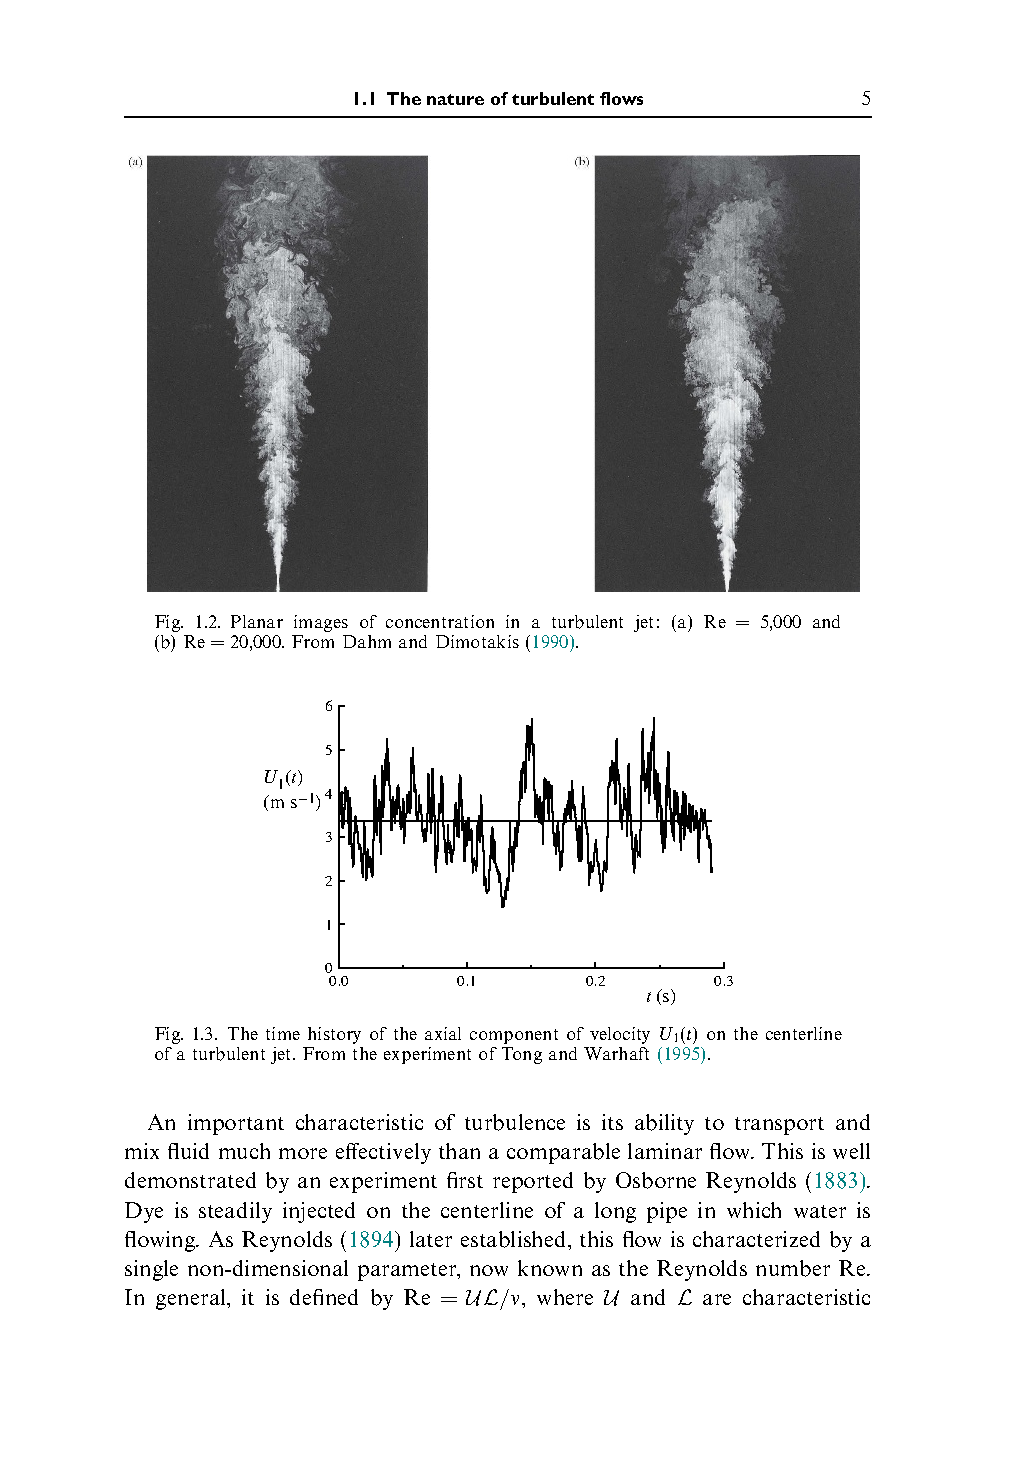
\includegraphics[width=0.8\linewidth,trim={4.3cm 7.7cm 4cm 11.5cm},clip]{Imagenes/03/turbulent}
	\caption{Serie de tiempo para una componente de la velocidad en un flujo turbulento. Fuente: Pope (2000) \cite{pope2000turbulent}.}
	\label{fig:03_turbulent}
\end{figure}

Para entender el origen de la turbulencia, consideremos el número de Reynolds:
\be Re = \frac{LD}{\nu}\ee
el cual se puede interpretar como el cuociente entre las fuerzas inerciales y viscosas en un fluido. Para un fluido que no es turbulento, o sea, laminar, el número de Reynolds es relativamente bajo y eso significa que la viscosidad predomina en su comportamiento. El rol que tiene la viscosidad acá es relevante, ya que es la encargada de atenuar perturbaciones que se puedan dar en las condiciones iniciales o de contorno. A medida que el número de Reynolds crece, la viscosidad irá perdiendo esta capacidad de atenuar las fluctuaciones y se llegará a un punto en donde estas fluctuaciones comenzarán a amplificarse localmente (se alcanza un número de Reynolds crítico y se entra en la zona de transición). A mayor número de Reynolds aún, es inevitable la presencia de inestabilidades en todo el flujo y es acá en donde se alcanza la turbulencia.

Actualmente no existe una definición formal de turbulencia. Luego, en ausencia de esta, se pueden presentar las principales características asociadas a los flujos turbulentos:
\begin{itemize*}
	\item La turbulencia es un proceso aleatorio
	\item La turbulencia contiene un amplio rango de diferentes escalas.
	\item La turbulencia presenta vorticidad aleatoria en pequeñas escalas.
	\item La turbulencia aparece a altos números de Reynolds.
	\item La turbulencia disipa energía.
	\item La turbulencia es un fenómeno del continuo.
	\item La turbulencia es un fenómeno tridimensional.
	\item Las grandes escalas de la turbulencia son insensibles a la viscosidad a altos número de Reynolds.
\end{itemize*}

A continuación se presentan dos de los resultados mas relevantes para el trabajo de tesis, con respecto a la teoría de la turbulencia homogénea e isotrópica.
\subsection{Aleatoriedad y Descomposición de Reynolds}
Reynolds en el año 1894 fue el primero en derivar un conjunto de ecuaciones para flujos turbulentos a través de la reconocida descomposición de Reynolds:
\be u_i = \overline{u}_i + u'_i \ee
Es decir, se descompone el campo de velocidad en una componente media y una componente fluctuante, de esta manera las ecuaciones que se solucionan serán aquellas para el flujo medio evitándose el problema de la aleatoriedad\footnote{El promedio acá se entiende como tanto espacial, temporal o de ensamble; haciendo uso de la teoría ergódica para turbulencia isotrópica homogénea desarrollada.}.

Aplicando esta descomposición junto con propiedades estadísticas del promedio y la conservación de masa, es posible escribir la ecuación de momentum (despreciando las fuerzas de cuerpo) de Navier-Stokes como:
\be\label{eq:03_cons_mom_rans}
(\partial_t \overline{u}_i + \overline{u}_j\partial_j \overline{u}_i)= \nu\partial_{jj}\overline{u}_i -\frac{1}{\rho}\partial_i \overline{p} + \partial_i(\overline{u'_iu'_j})
\ee
Notar que esta estructura es la misma que en la ecuación \ref{eq:cons_mom_nse} salvo que aparece un nuevo término $\overline{u'_iu'_j}$, el cual se le llama \textbf{esfuerzo de Reynolds} y corresponde a la covarianza de las velocidades.

El esfuerzo de Reynolds es el que acarrea la información sobre la turbulencia del flujo y tiene la característica de estar no cerrado, en el sentido que debe modelarse en función de las variables conocidas del problema o resolverla escribiendo una nueva ecuación de transporte para esta (introduciendo nuevas variables no cerradas). En dinámica atmosférica, generalmente la clausura se lleva a cabo utilizando esquemas sencillos que se verán en el próximo capítulo.

Con la introducción del tensor de esfuerzos de Reynolds, se puede definir ahora la energía cinética turbulenta $k$ (en adelante TKE) como:
\be k=\frac{1}{2}\overline{u'_i u'_i} \ee
\subsection{Escalas de la Turbulencia}
Para entender la manera en la que interactúan las distintas escalas presentes en la turbulencia, primero es necesario comprender el concepto de \emph{cascada de energía}. La idea de la cascada de energía fue introducida por Richardson en 1922, expone que la energía cinética entra a la turbulencia en las escalas mas grandes del movimiento. Esta energía es transferida (por un proceso no viscoso) a escalas cada vez mas pequeñas hasta que, en la escala mas pequeña posible, la energía es disipada por los efectos viscosos.

El mecanismo con el cual se lleva a cabo la cascada es la ruptura continua de vórtices. Los vórtices mas grandes son inestables (poseen un $Re$ elevado) y tienden a romperse en vórtices mas pequeños, estos vórtices continúan rompiéndose hasta que el número de Reynolds asociado a los vórtices se hace tan pequeño como para que la viscosidad pueda estabilizar sus estructuras.

La importancia de esta idea radica en que la disipación viscosa ocurre solamente al final de todo el proceso. Esta tasa de disipación $\varepsilon$ debe ser determinada entonces en el inicio de la cascada a través de la transferencia de energía de los vórtices más grandes.

La descripción analítica de las distintas escalas de la turbulencia se hizo por primera vez en 1941 por Kolmogorov a través de la postulación de tres hipótesis:
\paragraph{Hipótesis de Isotropía Local} A un número de Reynolds lo suficientemente elevado, los movimientos turbulentos de las pequeñas escalas son estadísticamente isotrópicos.
\paragraph{Primera Hipótesis de Similaridad} Para cualquier flujo turbulento a un número de Reynolds lo suficientemente elevado, las estadísticas de los movimientos de las pequeñas escalas tienen una forma universal y dependen solamente de $\nu$ y $\epsilon$.

Bajo esta hipótesis, es sencillo demostrar  por análisis dimensional que las pequeñas escalas $\eta$ serán del orden de:
\be \eta \sim \left( \frac{\nu^3}{\varepsilon}\right)^{1/4} \ee
Y su relación con las grandes escalas $l_0$:
\be \frac{\eta}{l_0}\sim Re^{-3/4} \ee
\paragraph{Segunda Hipótesis de Similaridad} Para cualquier flujo turbulento a un número de Reynolds lo suficientemente elevado, las estadísticas de los movimientos de las escalas ubicadas entre $l_0>l>\eta$ tienen una forma universal y dependen únicamente de $\varepsilon$, independiente de $\nu$.

De esta manera, un bosquejo típico log-log de la cascada de energía, se puede ver en la Figura \ref{fig:03_spectra}. Acá se grafica el espectro de energía $E$ en función del número de onda $\kappa$, es decir, cómo se distribuye la energía cinética a través de las distintas escalas espaciales ($\kappa\sim 1/l$).

\begin{figure}[h!]
	\centering
	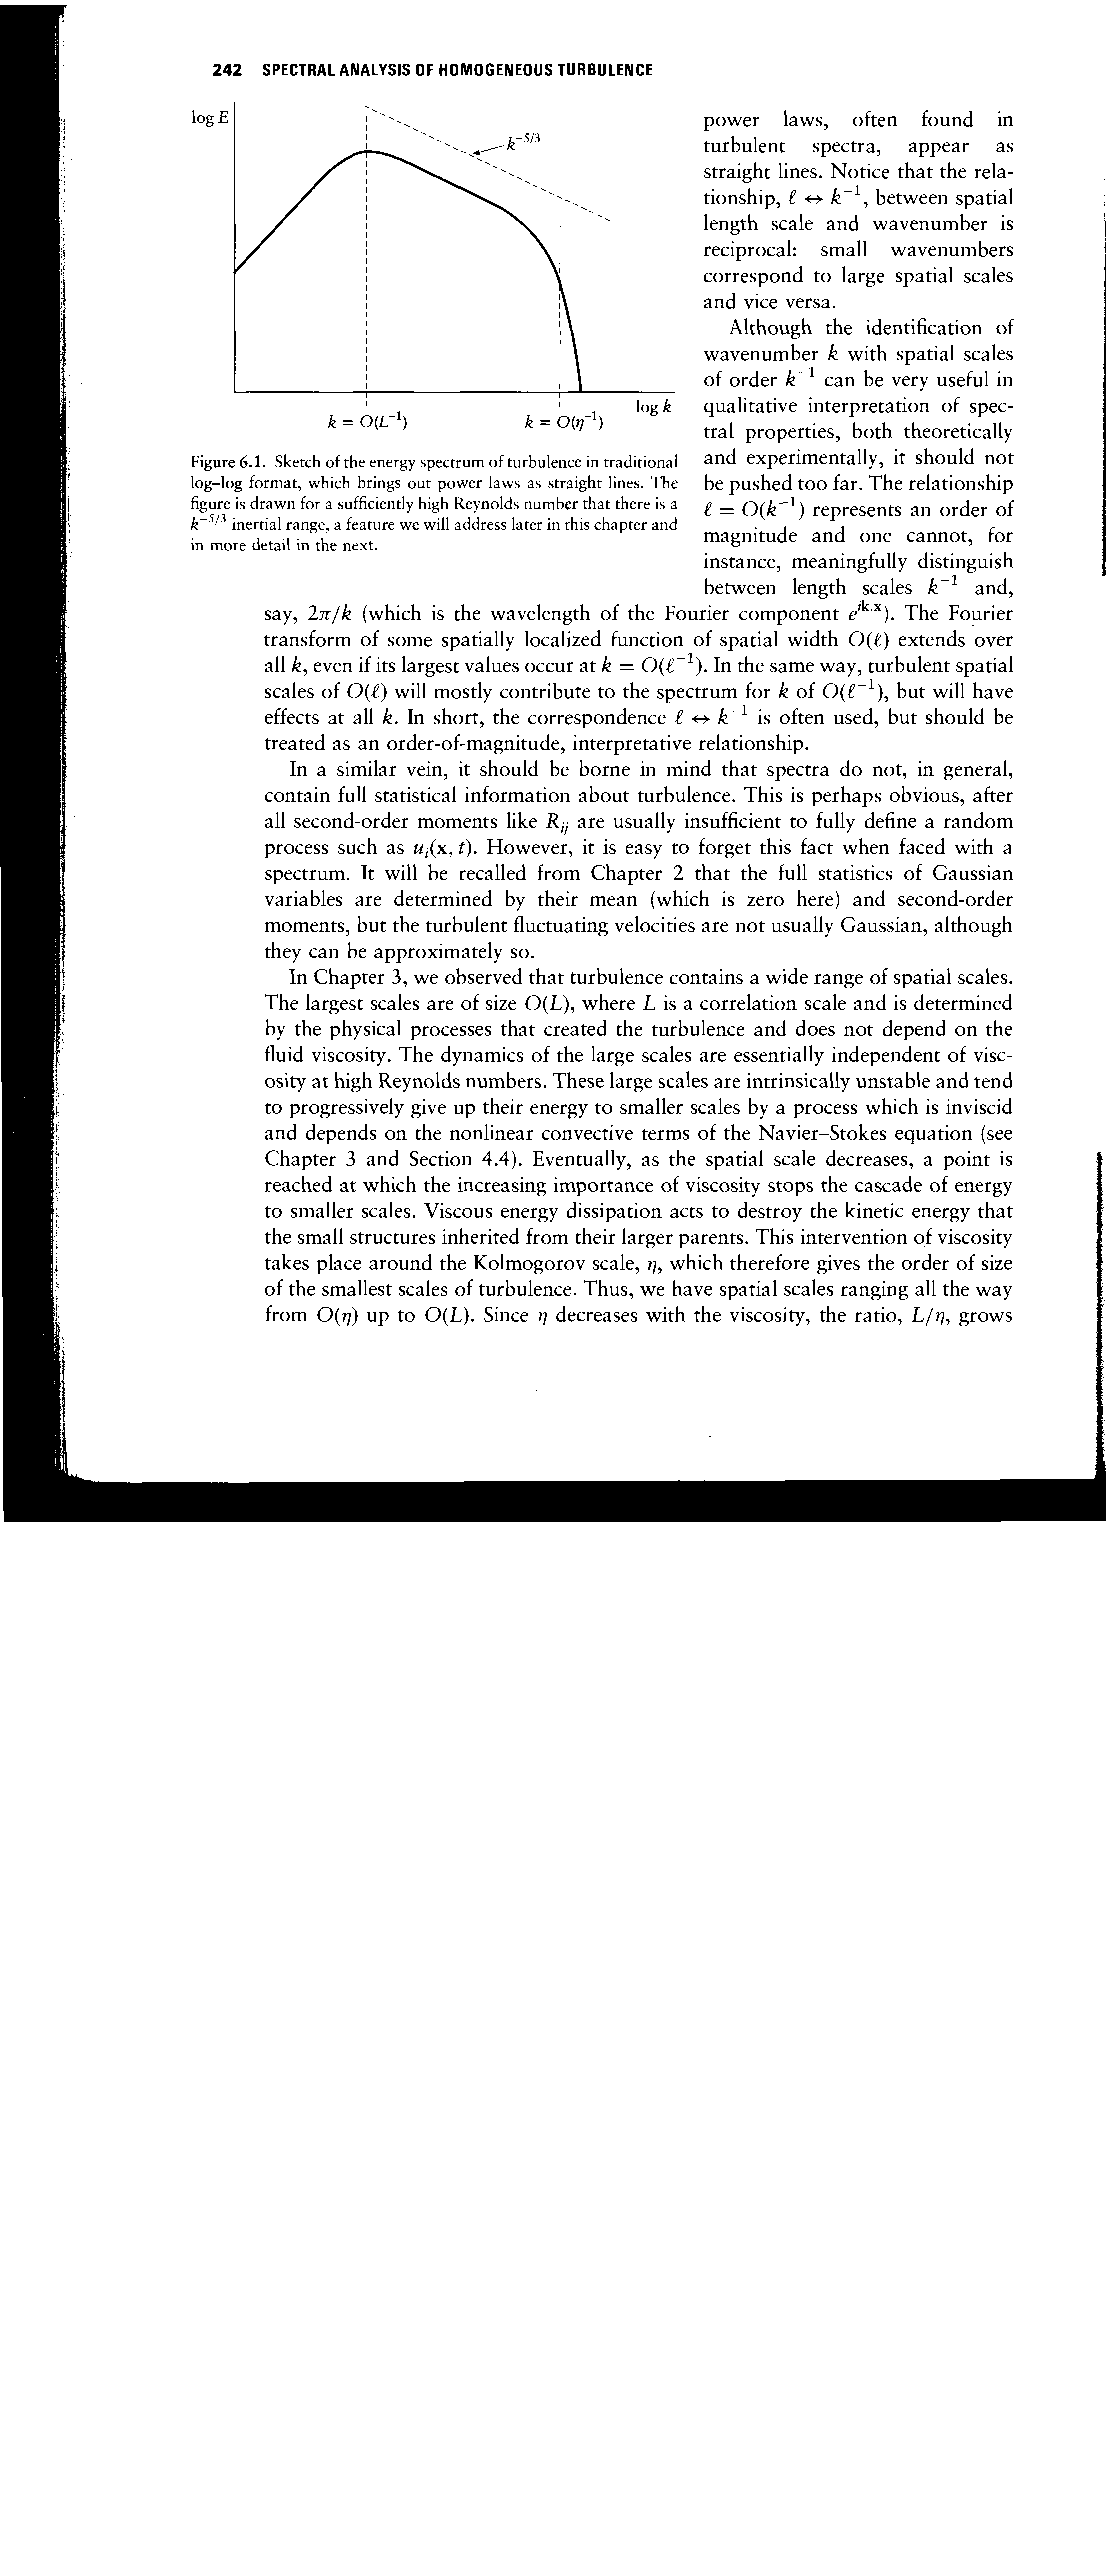
\includegraphics[width=0.85\linewidth,trim={3.2cm 18.3cm 7.0cm 1.5cm},clip]{Imagenes/03/spectra}
	\caption{Gráfico típico log-log de distribución de energía cinética turbulenta con respecto al número de onda $\kappa$ para un flujo con un número de Reynolds elevado. Fuente: Mathieu y Scott (2000) \cite{9780521775380}.}
	\label{fig:03_spectra}
\end{figure}

Tal como se explica anteriormente, existen tres zonas dentro de la cascada de energía. La primera, es la zona de producción de energía cinética asociada a lo grandes vórtices $l_0$. Luego, se ubica el rango inercial, el cual es solo función de la tasa de transferencia de energía y se comporta como una recta. Finalmente, está la microescala o escala de Kolmogorov $\eta$ donde ocurre la disipación.

Con respecto a la escala inercial, se puede demostrar por análisis dimensional que:
\be E(\kappa) = C\varepsilon^{2/3}\kappa^{-5/3} \ee
Este resultado nace de las consideraciones en las hipótesis de Kolmogorov. Se tiene entonces que para turbulencia homogenea e isotrópica, la pendiente (logarítmica) de la energía con respecto al número de onda en la escala inercial es universal y constante, y tiene un valor de -5/3.

De manera operacional, se puede encontrar el espectro de energía turbulenta haciendo una transformada de Fourier del campo de velocidades\footnote{Una definición mas formal del espectro, a través de las funciones de correlación, se puede ver en Mathieu y Scott (2000) \cite{9780521775380}.}. El par que define esta transformada será:
\be \tilde{u}'_i(\vec{\kappa},t) = \frac{1}{(2\pi)^3}\int u'_i(\vec{x},t) e^{-i\vec{\kappa}\cdot\vec{x}}d^3\vec{x} \ee
\be u'_i(\vec{x},t) = \int \tilde{u}'_i(\vec{\kappa},t) e^{-i\vec{\kappa}\cdot\vec{x}}d^3\vec{\kappa} \ee

El espectro de energía cinética turbulenta se puede expresar en función del número de onda $\vec{\kappa}$ como:
\be 
k = \frac{1}{2}\overline{u'_i u'_i} = \int\limits_0^\infty E(\kappa,t)d\kappa
\ee
\be
E(\kappa,t) = 2\pi\kappa^2\phi_{ii}(\kappa,t)
\ee 
\be 
\phi_{ii} \approx \overline{\tilde{u}'_i \tilde{u}'^*_i}
\ee
Acá $E$ es el espectro de energía, $\phi_{ii}$ es la transformada de Fourier de la llamada función de correlación (que en esta formulación funciona como variable auxiliar) y el superíndice $^*$ denota el conjugado.

\newpage 
\section{Fundamentos de Capa Límite Atmosférica}
Se define la capa límite atmosférica (ABL \emph{Atmospheric Boundary Layer} o PBL \emph{Planetary Boundary Layer}) como la parte de la troposfera que está influenciada directamente por la presencia de la superficie terrestre y que responde a las fuerzas superficiales en una escala de tiempo del orden de las horas o menor.

La ABL es altamente variable y se caracteriza por ser turbulenta en la gran mayoría de los casos. Su turbulencia es generada debido al roce con la superficie, la presencia de obstáculos y/o por flotación debido a la temperatura del suelo. 

Existe una estructura bien definida para las capas límites atmosféricas que se desarrollan sobre superficies a alta presión, esta estructura es variable en el tiempo, siendo influenciada principalmente por los ciclos diarios de enfriamiento y calentamiento de la superficie por la radiación solar. En la Figura \ref{fig:03_abl}\footnote{\url{https://commons.wikimedia.org/wiki/File:Atmospheric\_boundary\_layer.svg}} se puede ver la evolución de la estructura de la capa límite en las distintas horas del día (para un día estándar) y sus principales componentes.

\begin{figure}[h!]
	\centering
	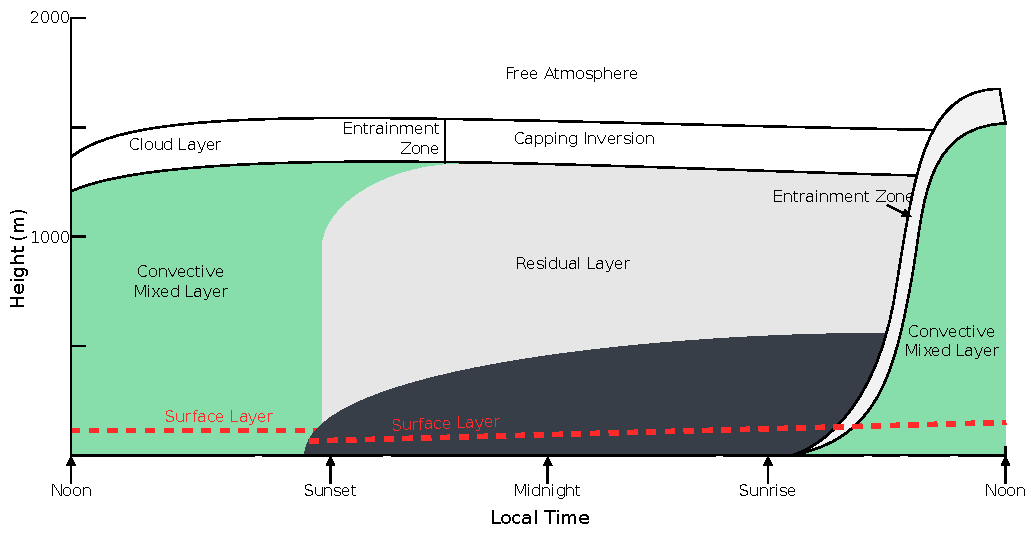
\includegraphics[width=0.98\linewidth,trim={0cm 0cm 0cm 0cm},clip]{Imagenes/03/abl}
	\caption{Evolución diurna de la estructura de la capa límite. Fuente: Wikimedia.}
	\label{fig:03_abl}
\end{figure}

Como se puede ver, la ABL posee 3 grandes componentes: (a) la capa de mezcla o \emph{mixed layer} (b) la capa residual o \emph{residual layer} y (c) la capa límite estable o \emph{stable boundary layer} (en negro). Además de estas, se reconoce la capa de superficie o \emph{surface layer} que es la región al fondo de la capa límite donde los esfuerzos turbulentos no varían mas de un 10\% de su magnitud y que es dominada principalmente por el roce con el terreno. Así, sea cual sea la estructura de la capa límite, el 10\% mas cercano a la superficie va a corresponder siempre a la capa superficial. Finalmente, una capa delgada llamada microcapa o capa de interfaz se ubica en los primeros centímetros de la capa de aire. En esta, el transporte molecular (viscosidad) predomina sobre el transporte turbulento.

Algunas características esenciales de la ABL se mencionan a continuación:
\begin{itemize*}
	\item La humanidad gasta la mayoría de su vida dentro de la ABL.
	\item Los pronósticos del clima son en verdad pronósticos de la capa límite.
	\item La polución queda atrapada en la ABL.
	\item La neblina es creada en la ABL.
	\item La fuente principal de energía para toda la atmósfera es la radiación solar, la cual, en su mayoría es absorbida por el suelo y transmitida al resto de la atmósfera por los procesos de capa límite.
	\item Cerca de un 50\% de la energía cinética de la atmósfera es disipada en la capa límite.
	\item El transporte turbulento de momemtum desde la capa límite a la superficie es el sumidero mas grande de momemtum de la atmósfera.
	\item Las turbinas eólicas extraen energía de los vientos de la ABL.
\end{itemize*}
\subsection{Estructuras de Capa Límite}
\subsubsection{Capa de Mezcla}
Se caracteriza por poseer una turbulencia que usualmente es provocada por la convección, aunque es posible que se forme una especie de capa de mezcla en zonas con vientos fuertes. Las fuentes de convección incluyen la transferencia de calor desde la superficie caliente y el enfriamiento por radiación desde la parte superior de una capa de nubes. La primera de estas, crea movimientos de aire caliente ascendentes desde la superficie de la tierra, mientras que la segunda, genera movimientos descendentes de aire frío desde las nubes. Ambos puedes ocurrir simultáneamente.

En días despejados, el crecimiento de la capa de mezcla está unido al calentamiento solar de la superficie. Comenzando aproximadamente media hora después del amanecer, la altura de la capa de mezcla turbulenta empieza a crecer. La característica fundamental de la capa de mezcla es la mezcla intensa de las variable atmosféricas dentro de esta debido a su condición de ser estáticamente inestable a causa del ascenso de aire caliente. La capa de mezcla alcanza su máxima altura después del mediodía.

Los perfiles de temperatura potencial virtual para esta capa suelen ser generalmente adiabáticos debido a la mezcla, mientras que en la capa superficial es normal hallar perfiles superadiabáticos debido a la superficie caliente.

Sobre la capa de mezcla, una capa estable actua como cubierta de los movimientos ascendentes de aire caliente restringiendo el dominio de la turbulencia. Es la llamada capa de arrastre o \emph{entrainment zone}. Generalmente esta capa es lo suficientemente estable como para que ocurra una inversión térmica y por lo tanto, también se le denomina como capa de inversión.

La rapidez de los vientos dentro de esta capa son subgeostróficos. La parte media de la capa de mezcla presenta un perfil de velocidad que es casi constante (debido a la alta mezcla de momemtum) y un perfil logarítmico en los dominios de la capa de superficie.

\subsubsection{Capa Residual}
En ausencia de advección de aire frío, aproximadamente media hora antes del atardecer, las corrientes ascendentes calientes dejan de existir y la turbulencia en la capa de mezcla decae. La capa de aire que queda se le llama capa residual. Esta capa es de estratificación neutra, lo que implica que la turbulencia es casi de la misma magnitud en todas las direcciones y su perfil de $\theta_v$ es casi adiabático.

Los escalares pasivos que flotaron gracias a la radiación del día se mantendrán en el aire en la capa residual y en el amanecer, cuando la capa de mezcla comienza a arrastrarse con la capa residual, la radiación solar puede provocar reacciones fotoquímicas sobre estos escalares. Esto tiene especial importancia para el caso de la humedad (que se puede considerar a grandes rasgos como un escalar pasivo). En la capa de mezcla la humedad se evapora y quedará retenida dentro de la capa residual, con el pasar de los días, la unificación de la capa residual con la capa de mezcla puede generar formación de nubes en zonas donde, de otra manera, no se podría.

La capa residual no tiene contacto directo con la superficie. Durante la noche, la capa estable aumenta su espesor modificando el fondo de la capa residual. Luego, la capa residual no es afectada por el transporte turbulento de propiedades relacionadas a la superficie y por lo tanto no cae dentro de la definición de lo que se define como capa límite, sin embargo es una estructura dominante de la atmósfera.
\subsubsection{Capa Límite Estable}
A medida que la noche progresa, la parte inferior de la capa residual se transforma debido al contacto con la superficie en una capa límite estable. Esta se caracteriza por ser estáticamente estable y poseer de manera esporádica turbulencia de baja intensidad. Si bien los vientos a nivel de superficie se vuelven mas tranquilos, por sobre esto, el viento puede acelerar a velocidades supergeostróficas en un fenómeno llamado jet nocturno o corriente en chorro de bajo nivel.

Mientras que el aire estáticamente estable tiende a suprimir la producción de turbulencia a nivel de superficie, el desarrollo del jet nocturno fomenta el cortante en el viento, lo cual incita la turbulencia lejos de la superficie. Como resultado, existe turbulencia que se manifiesta en ráfagas cortas que generan mezcla a lo largo de la capa límite estable. Durante los periodos no turbulentos, el movimiento del viento se desacopla de la superficie.

El límite superior de la capa límite estable no es fácilmente identificable como lo es en la capa de mezcla, ya que esta se une suavemente a la capa residual. El largo de la capa estable será la altura en donde la turbulencia es solo una pequeña fracción de su valor superficial.

La velocidad del viento en la noche tiene un comportamiento complejo. En las cercanias de la superficie generalmente se tiene un viento leve o incluso calmado. Sobre los 200 [m] el aire puede alcanzar velocidades de entre 10 a 30 [m/s] en el jet nocturno. Unos cuantos cientos de metros mas arriba y la velocidad del viento disminuye, recuperando su valor geostrófico.

Esta capa estable también es posible que se forme en el día siempre y cuando la superficie sea mas fría que el aire que lo rodea, como puede ser el caso de frentes cálidos o zonas cercanas a la costa.
\subsubsection{Evolución de la Temperatura Potencial}
En la Figura \ref{fig:03_pbl2} se muestra la evolución para la temperatura potencial virtual $\theta_v$ a lo largo de un día estándar. Se puede observar que el perfil de $\theta_v$ da la información suficiente para reconocer perfectamente la estructura de la capa límite. 
\begin{figure}[h!]
	\centering
	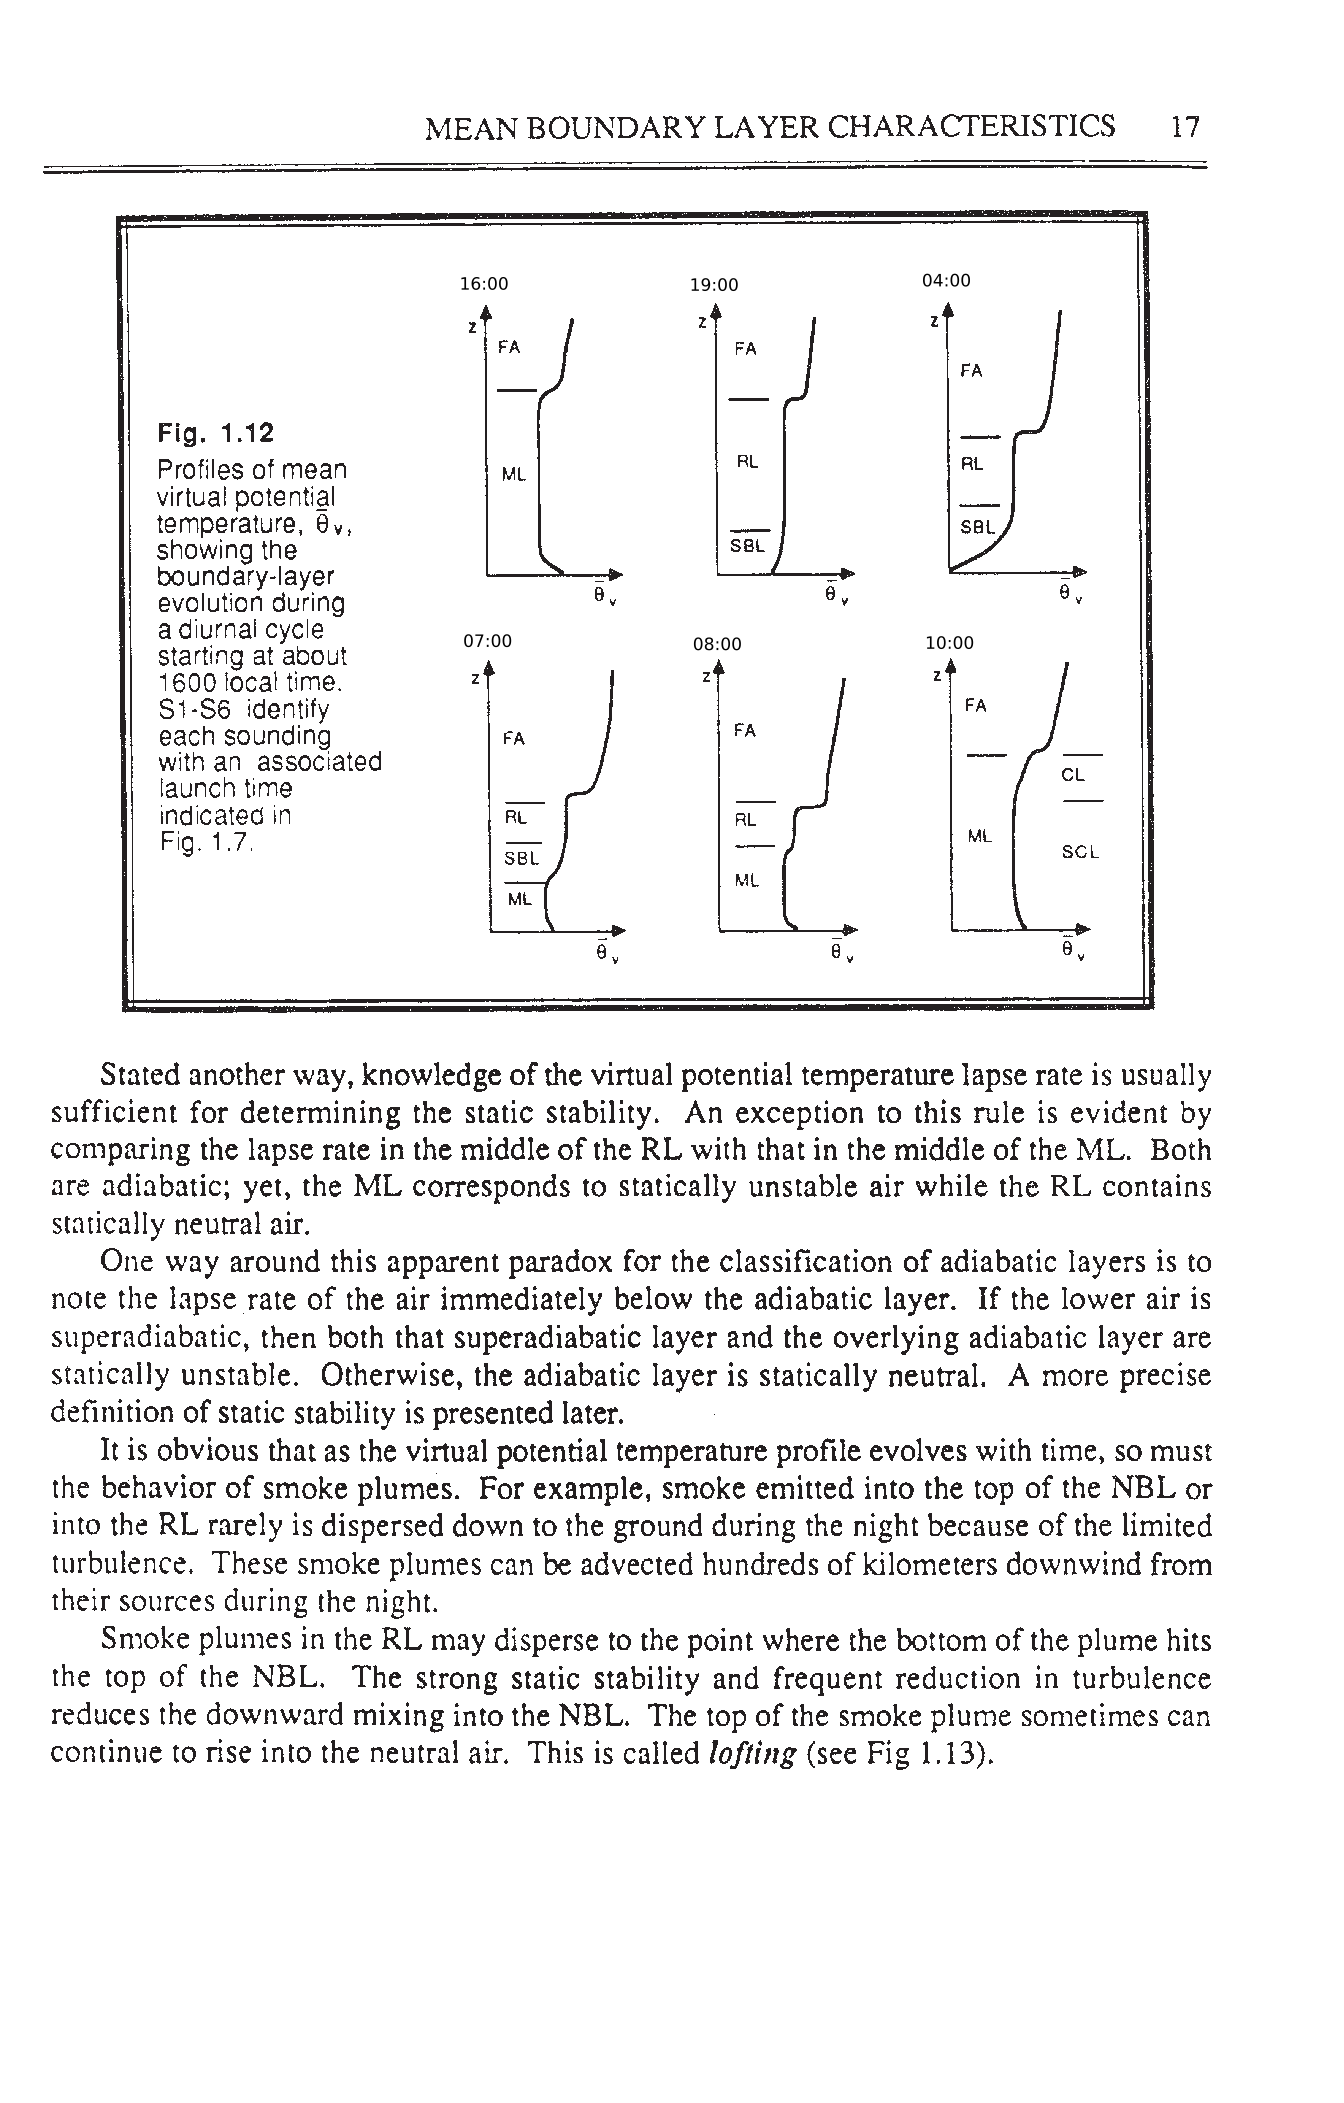
\includegraphics[width=0.7\linewidth,trim={5.6cm 14cm 2.7cm 3.3cm},clip]{Imagenes/03/pbl2}
	\caption{Evolución del perfil de $\theta_v$ en el ciclo diurno. Fuente: Stull (1988) \cite{stull1988introduction}.}
	\label{fig:03_pbl2}
\end{figure}

En esta figura se usan los siguientes acrónimos:
\begin{itemize*}
	\item FA: \emph{Free Atmoshere}, atmósfera libre.
	\item ML: \emph{Mixed Layer}, capa de mezcla.
	\item RL: \emph{Residual Layer}, capa residual.
	\item SBL: \emph{Stable Boundary Layer}, capa límite estable.
	\item CL: \emph{Cloud Layer}, capa de nubes.
	\item SCL: \emph{Subcloud Layer}, capa de subnubes.
\end{itemize*}
\subsection{Esfuerzos Turbulentos}
La turbulencia mezcla momemtum, energía, humedad y contaminantes vertical y horizontalmente. El grado de turbulencia puede ser cuantificado en un término de flujo turbulento (tal como se detalló en la sección anterior). Para el caso del momemtum horizontal, el flujo turbulento vertical será una función de $\overline{w'u'}$ y $\overline{w'v'}$, que son los flujos turbulentos cinemáticos verticales medios.

Los flujos turbulentos cinemáticos medios son negativamente proporcional a los esfuerzos de Reynolds. Este esfuerzo hará que una parcela de aire sufra una deformación. Consideremos el caso vertical en dirección $x$: la velocidad $w'$ generará mezcla de la velocidad $u'$ . La mezcla vertical de $u'$ producirá un esfuerzo en la dirección $x$ y normal a $z$. Este esfuerzo se calcula como:
\be 
\tau_{R,xz} = - \rho \overline{w'u'}
\ee
Ahora, generalmente se quiere saber el esfuerzo total generado por el movimiento horizontal, el cual es relevante a bajas alturas. Se puede demostrar que se puede escribir el flujo turbulento vertical de momemtum horizontal como:
\be 
|\tau_{R,z}| = \rho[(\overline{w'u'})^2 + (\overline{w'v'})^2]^{1/2}
\ee
Coloquialmente a $\tau_{R,z}$ se le conoce también $\tau_{13}$ en la literatura, referenciando a $1$ como la dirección horizontal del viento y $3$ la dirección vertical.

De la misma manera, los flujos turbulentos verticales causan mezcla turbulenta de calor y de humedad desde la superficie. Se pueden anotar estos como:
\be H_f = \rho C_{p,d} (\overline{w'\theta_v'})_s \ee
\be Q_f = \rho (\overline{w'q_v'})_s \ee
\subsubsection{Velocidad de Fricción}
En el contexto de la parametrización de los esfuerzos turbulentos de la superficie, es conveniente introducir una nueva variable de escalamiento para la velocidad que permita reducir el problema. Esta es la llamada velocidad de fricción. Se calcula como:
\be u_* = \sqrt{\frac{|\tau_{R,z}|}{\rho}} \ee
$u_*$ es una métrica de la turbulencia producida mecánicamente debido al roce, al cortante y a la presencia de protuberancias en el terreno.
\subsubsection{Clausura de la Difusión Turbulenta}
La formulación de ecuaciones de transporte para los flujos turbulentos introduce mas incógnitas que ecuaciones. Es necesario entonces, buscar una manera de lograr la clausura del problema introduciendo alguna relación adecuada. Para los flujos en la capa superficial, sea de momemtum, calor, humedad, etc., estos suelen ser estimados mediante la aplicación de: (a) fórmulas para el arrastre aerodinámico (orden 0), (b) teoría de similaridad de Monin-Obukhov (orden 0), (c) teoría del transporte gradiente (orden 1) o (d) teorías con formulaciones de orden superior.

En la formulación de arrastre se tiene:
\be 
(\overline{w'u'})_s = -C_D|\overline{V}_h(z_r)|[\overline{u}(z_r) - \overline{u}(z_{0,m})]
\ee 
$z_{0,m}$ es el largo de rugosidad para la similaridad de momemtum. Notar que $\overline{u}(z_{0,m}) = 0$ por definición. $z_r$ es una altura de referencia (generalmente 10 [m]) y $C_D$ es el coeficiente de arrastre a la altura de referencia.

En la formulación de transporte gradiente se tiene un coeficiente de difusión turbulento de la forma:
\be 
K_{m,zx} = -\frac{(\overline{w'u'})_s}{\partial \overline{u}/\partial z } = C_D |\overline{V}_h(z_r)|(z_r - z_{0,m})
\ee 

Las teorías de arrastre aerodinámico y de transporte gradiente son bien conocidas en el área de la mecánica de fluidos y por lo tanto no trae mayor beneficio el detallarlas acá. Por otro lado, la teoría de similaridad de Monin-Obukhov presenta una mayor intuición acerca del comportamiento de la capa límite y es relevante presentar sus fundamentos, ya que en base a esta se desarrollan la mayoría de los solvers atmosféricos.

\subsubsection{Teoría de Similaridad de Monin-Obukhov}
Se habla de teoría de Monin-Obukhov al referirse a la aplicación de la teoría de similaridad (grupos adimensionales) a la capa límite atmosférica considerando tantos los efectos de roce, como los efectos de flotación.

Una primera relación adimensional que nace de este acercamiento es el gradiente de viento adimensional:
\be \label{eq:03_simi_u}
\frac{\phi_m}{\kappa} = \frac{z}{u_*}\frac{\partial |V_h|}{\partial z}
\ee
Donde $\phi_m$ es un valor que se calcula en función de $z/L$, siendo $L$ es el largo de Monin-Obukhov. $\kappa$ es la constante de Von Karman (usualmente 0,4). Businger et al. (1971) presenta la función de $\phi_m$ de la forma:

\be 
\phi_m = \begin{cases}
	1+\beta_m \frac{z}{L} & \frac{z}{L}>0  \quad\text{estable}\\
	(1-\gamma_m \frac{z}{L})^{-1/4} & \frac{z}{L}<0 \quad \text{inestable}\\
	1 & \frac{z}{L}=0  \quad \text{neutral}
\end{cases}
\ee 
Acá $\beta_m$ y $\gamma_m$ son constantes en función del valor de $\kappa$ que se use \cite{jacobson2005fundamentals}.

El largo de Monin-Obukhov $L$ es una altura proporcional a la altura a la cual la producción de turbulencia debido a la flotación comienza a dominar por sobre la producción debido a efectos mecánicos. Matemáticamente,
\be 
L = \frac{u_*^3\overline{\theta}_v}{\kappa g (\overline{w'\theta'_v})_s} = \frac{u_*^2 \overline{\theta}_v}{\kappa g \theta_*}
\ee 
La segunda igualdad es obtenida sustituyendo por la siguiente relación de similaridad,
\be 
(\overline{w'\theta'_v})_s \approx -u_* \theta_*
\ee
Acá se introduce $\theta_*$ que es una variable de escalamiento para la temperatura potencial\footnote{Se omitirá la manera de aproximar $\theta_*$ en este documento, sin embargo se motiva al lector a leer la referencia \cite{jacobson2005fundamentals} si desea conocer mas al respecto.}. $\theta_*$ es proporcional a la diferencia vertical de temperatura potencial. A mayor valor de $\overline{\theta}$ en la cercanía de la superficie, más negativo será el cambio de temperatura potencial con respecto a la altura y por ende mas inestable será la atmósfera. Para este caso $L$ será negativo pero de un valor pequeño (es inversamente proporcional a $\theta_*$). Si $L$ es pequeño y negativo, $z/L$ es negativo y grande. Estos valores de $z/L$ corresponden a atmósferas inestables debido a la flotación. Análogamente, valores positivos de $z/L$ corresponden a atmósferas estables.

Evidentemente, la introducción de $\theta_*$ permite escribir relaciones de similaridad para el perfil de $\theta$ de la forma:
\be \label{eq:03_simi_theta}
\frac{\phi_h}{\kappa} = \frac{z}{\theta_*}\frac{\partial \overline{\theta}_v}{\partial z}
\ee

\be 
\phi_h = \begin{cases}
	\text{Pr}_t+\beta_h \frac{z}{L} & \frac{z}{L}>0  \quad\text{estable}\\
	\text{Pr}_t(1-\gamma_h \frac{z}{L})^{-1/2} & \frac{z}{L}<0 \quad \text{inestable}\\
	\text{Pr}_t & \frac{z}{L}=0  \quad \text{neutral}
\end{cases}
\ee
Pr$_t$ es el número de Prandtl turbulento, calculado como la razón entre los coeficientes de difusión turbulentos de momemtum $K_m$ y de energía $K_h$ . Para $\kappa=0.4$ se estima un valor de Pr$_t\approx 0.95$.

Todo este desarrollo permite escribir los coeficientes de difusión turbulenta en función de la teoría de similaridad como,
\be 
K_{m,zx} = \frac{\kappa z u_*}{\phi_m}
\ee 
\be 
K_{h,zx} = \frac{\kappa z u_*}{\phi_h}
\ee 

Finalmente, utilizando la teoría de similaridad es posible derivar los perfiles verticales de viento y temperatura potencial virtual (humedad también, pero se ha omitido en este desarrollo). Integrando las ecuaciones \ref{eq:03_simi_u} y \ref{eq:03_simi_theta} se tiene que:
\be 
|\overline{V}_h(z)| = \frac{u_*}{\kappa} \left[ \ln\left( \frac{z}{z_{0,m}} - \psi_m \right) \right]
\ee
\be 
\overline{\theta}_v(z) = \overline{\theta}_v(z_{0,h}) + \text{Pr}_t \frac{\theta_*}{\kappa} \left[ \ln\left( \frac{z}{z_{0,h}} - \psi_h \right) \right]
\ee
Donde:
\be 
\psi_m = \int\limits_{z_{0,m}}^{z}  (1-\phi_m)\frac{dz}{z}\quad;\quad \psi_h = \int\limits_{z_{0,m}}^{z}  (1-\phi_h)\frac{dz}{z}
\ee
Son las funciones de influencia para momemtum y energía que permiten adecuar el perfil logaritmico según la estratrificación. 

Para condiciones neutras se tiene que $\phi_m = 1$ y el perfil de viento horizontal se reduce a su forma:
\be 
|\overline{V}_h(z)| = \frac{u_*}{\kappa} \ln \frac{z}{z_{0,m}}
\ee
la cual es una fórmula clásica para estimar la velocidad del viento dentro de la capa límite.
\subsection{Ecuación de Energía Cinética Turbulenta}
La ecuación de transporte que rige el comportamiento del TKE se puede escribir de la siguiente forma \cite{stull1988introduction}:
\be
\partial_t k + \overline{u}_j\partial_j k = \delta_{i3}\frac{g}{\overline{\theta}_v}\overline{u'_i\theta'_v} - \overline{u'_i u'_j} \partial_j \overline{u_i} - \partial_j\overline{u'_j k} - \frac{1}{\rho} \partial_i \overline{u'_i p'} - \varepsilon
\ee
Donde $\varepsilon$ es la disipación viscosa de energía cinética turbulenta:
\be  \varepsilon = \nu(\overline{\partial_j u'_i\partial_j u'_i}) \ee

Para ganar intuición acerca de los distintos términos presentes en la ecuación, es conveniente tomar un sistema coordenado alineado con la dirección del viento medio y asumir homogeneidad horizontal, además se desprecia la advección relacionada a la componente vertical. De esta manera una forma especial del balance de TKE se puede escribir como:
\newpage
\be
\partial_t k  = \frac{g}{\overline{\theta}_v}\overline{w'\theta'_v} - \overline{u' w'} \partial_z \overline{u} - \partial_z\overline{w' k} - \frac{1}{\rho} \partial_z \overline{w' p'} - \varepsilon
\ee
\vspace{-7mm}
\begin{equation*}
\quad I \quad\qquad II\quad\qquad III\qquad\qquad IV\quad\qquad V\quad\qquad VI
\end{equation*}
El significado físico de cada término es:
\begin{enumerate*}
	\item[I.] Acumulación local o tendencia de TKE.
	\item[II.] Producción o consumo debido a flotación.
	\item[III.] Producción mecánica por cortante.
	\item[IV.] Transporte turbulento de TKE.
	\item[V.] Correlación de presión, describe la distribución de TKE debido a perturbaciones de presión (por flotación o ondas de gravedad).
	\item[VI.] Disipación de TKE.
\end{enumerate*}

Como síntesis, la turbulencia es disipativa. El término $VI$ existe siempre que el TKE no sea cero. Físicamente, esto significa que la turbulencia tiende a decaer y desaparecer a través del tiempo, a no ser que sea creada localmente o trasportada por el flujo medio o procesos turbulentos o de presión. Luego, el TKE no es una cantidad que se conserva. La capa límite puede ser turbulenta solo si existen ciertos procesos físicos generando esta turbulencia.

Las Figuras \ref{fig:03_tke3}, \ref{fig:03_tke1} y \ref{fig:03_tke2} (Fuente: Stull, 1998 \cite{stull1988introduction}) representan la distribución de TKE y el balance de los términos de la ecuación de TKE\footnote{Acá se utiliza una nueva variable de escalamiento $w_*$. Corresponde a una velocidad de escalamiento convectiva. Se calcula como: $[(g\delta/\overline{\theta}_v)(\overline{w'\theta'_v})_s]^{1/3}$.} para distintas horas de un día según simulaciones de varios autores. Estos gráficos y valores servirán de referencia a los valores obtenidos en los resultados de los experimentos de esta tesis.

\begin{figure}[h!]
	\centering
		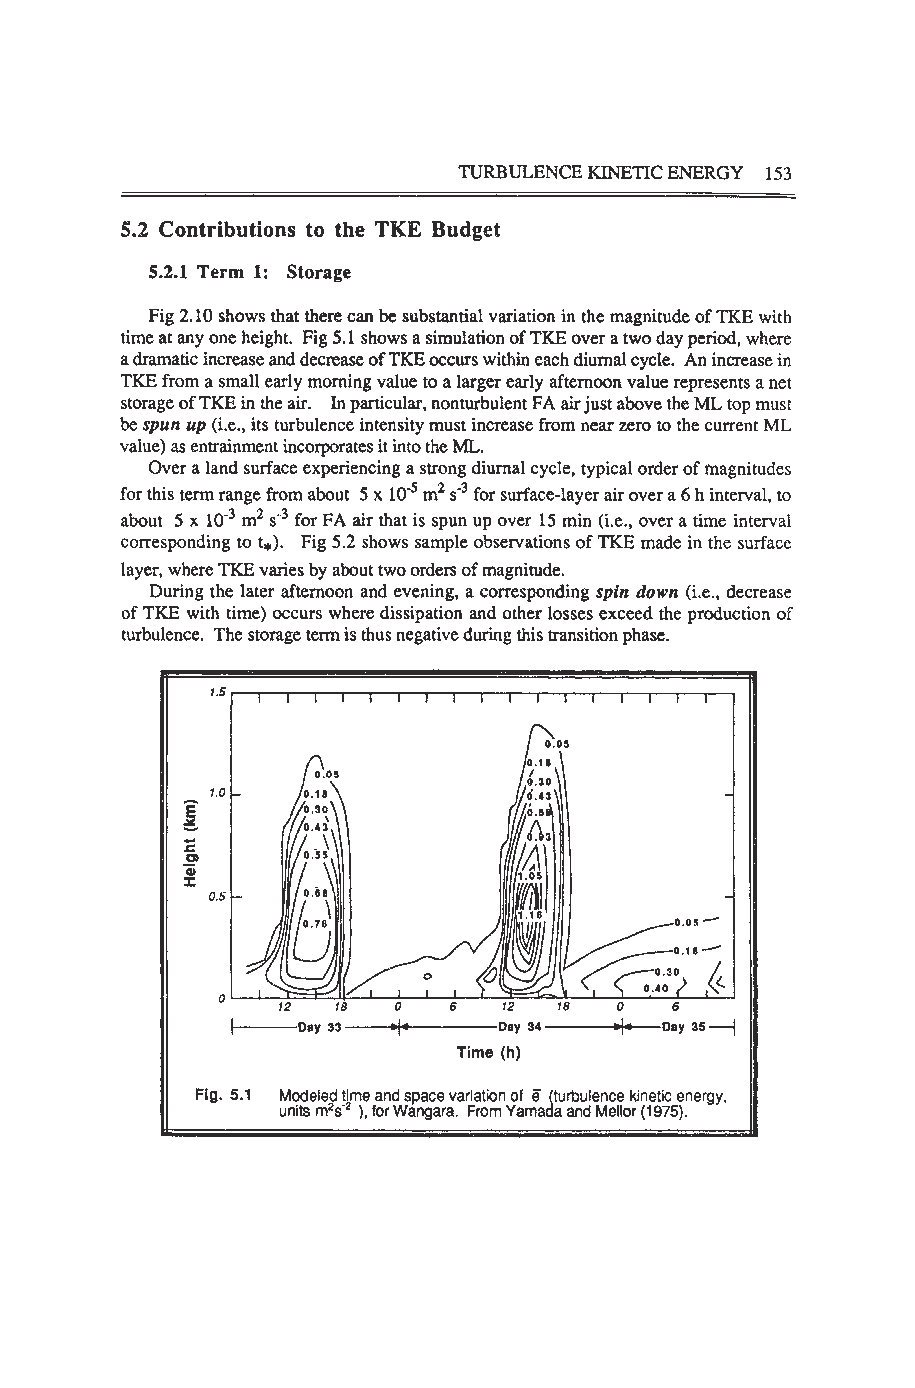
\includegraphics[width=0.8\linewidth,trim={3cm 5.5cm 2.9cm 11.6cm},clip]{Imagenes/03/tke3}
	\caption{Variación espacial y temporal de TKE modelada. Fuente: Stull (1988) \cite{stull1988introduction}.}
	\label{fig:03_tke3}
\end{figure}

La Figura \ref{fig:03_tke3} muestra como el valor del TKE es alto a nivel de superficie y tiende a decaer con la altura. En atmósferas inestables, como lo es a mitad del día, el perfil crece y se obtienen grandes valores para el TKE. Las Figuras \ref{fig:03_tke1} y \ref{fig:03_tke2} muestran como en el día la generación de TKE está dominada por los efectos de flotación y de corte en las zonas muy cercanas a la superficie, y en la noche, estos mecanismos se calman dando espacio a que la disipación actue como sumidero de TKE. Notar el cortante que se genera lejos de la superficie debido al jet nocturno.

\begin{figure}[h!]
	\centering
	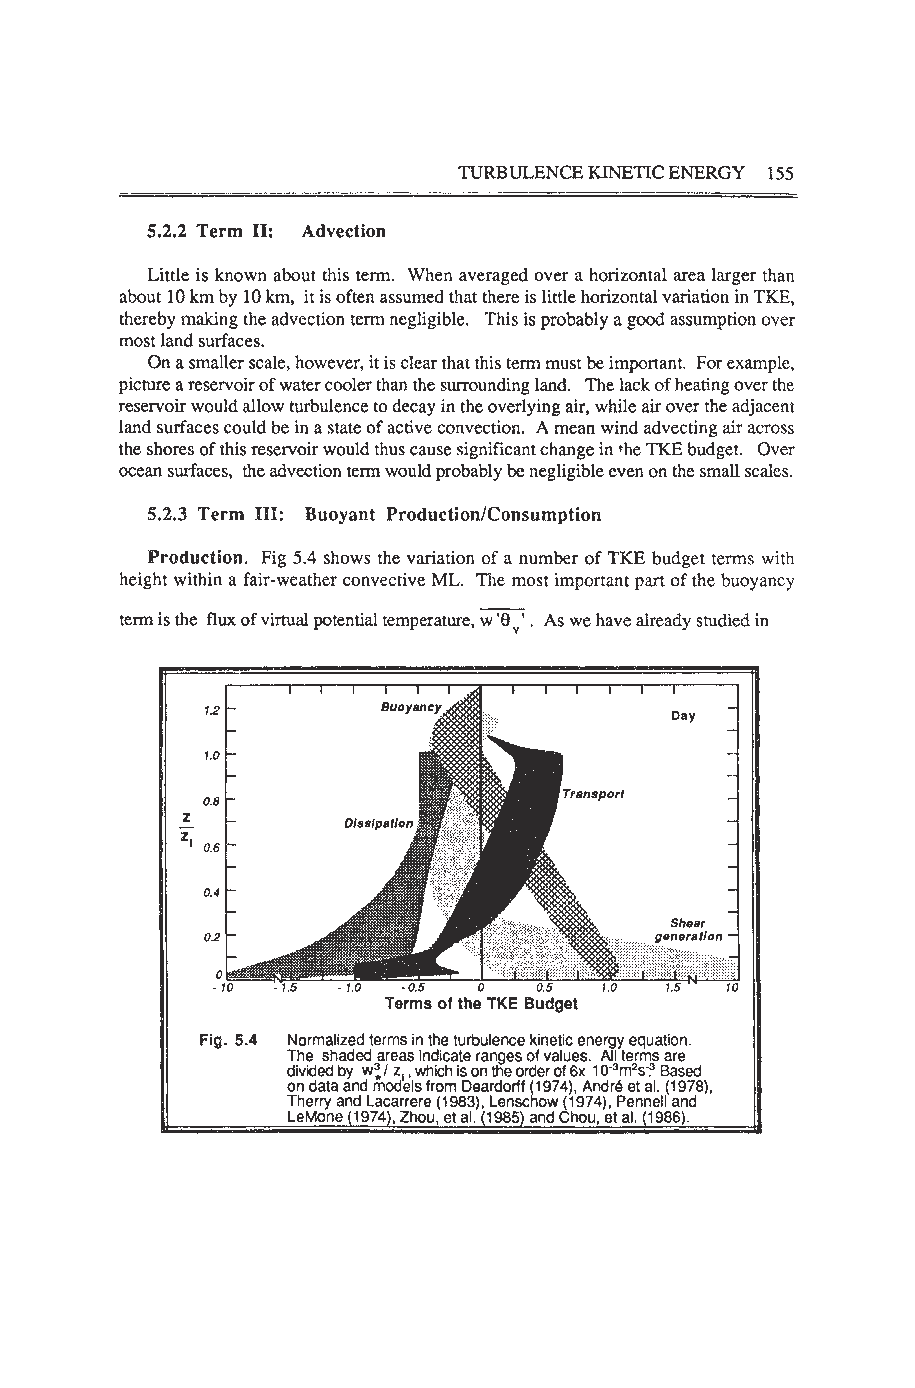
\includegraphics[width=0.8\linewidth,trim={3cm 6.3cm 2.9cm 11.5cm},clip]{Imagenes/03/tke1}
	\caption{Términos normalizados en la ecuación de TKE para el día. Las áreas sombreadas corresponden a un rango de valores. Todos los términos son adimensionalizados por $w_*^3/\delta$. Fuente: Stull (1988) \cite{stull1988introduction}.}
	\label{fig:03_tke1}
\end{figure}

\begin{figure}[h!]
	\centering
		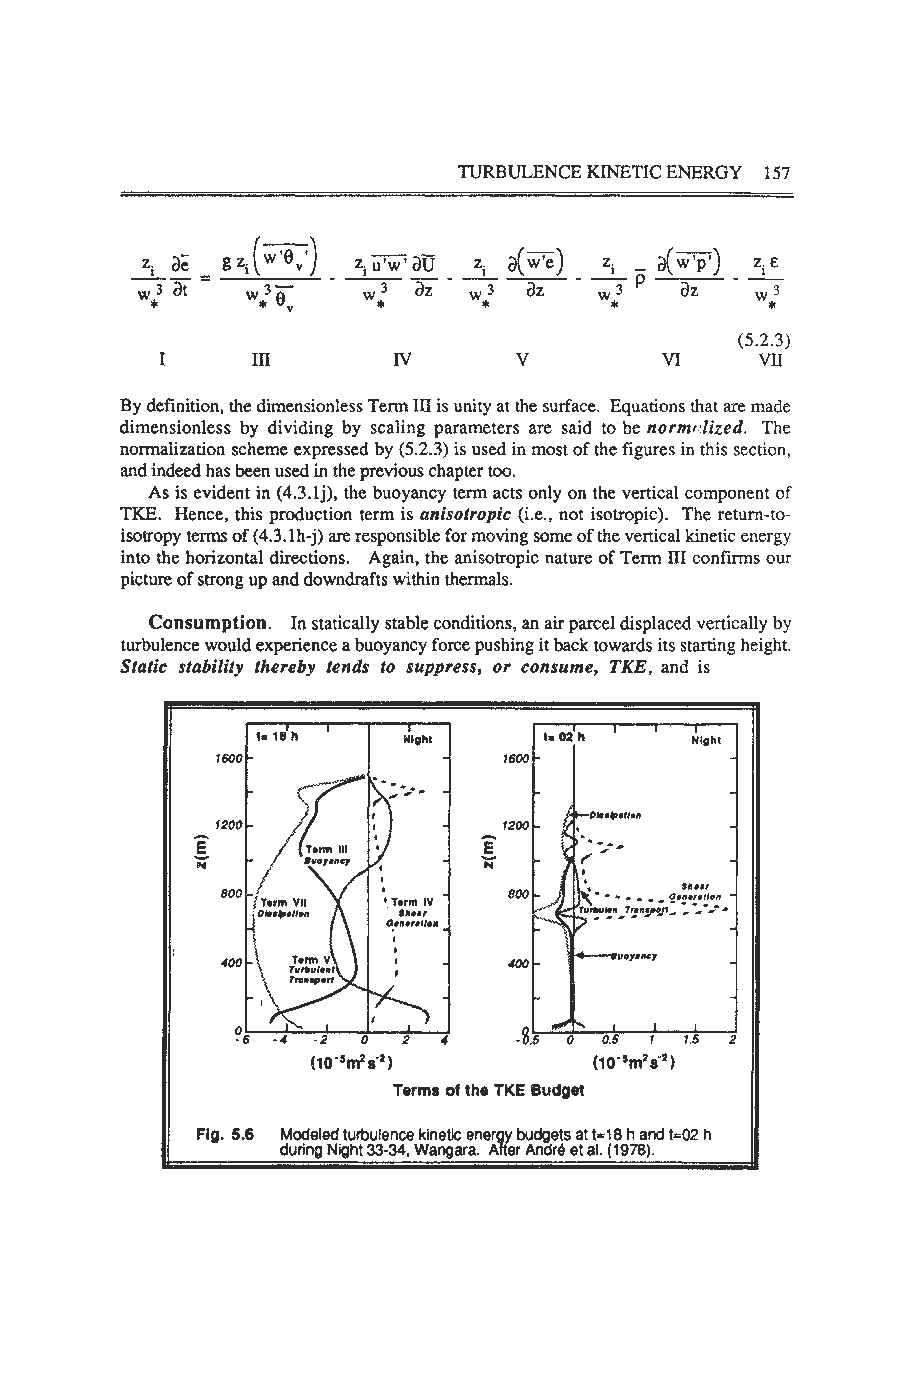
\includegraphics[width=0.8\linewidth,trim={3.2cm 4.8cm 2.8cm 12.1cm},clip]{Imagenes/03/tke2}
	\caption{Términos normalizados en la ecuación de TKE para la noche (18:00 y 02:00). Fuente: Stull (1988) \cite{stull1988introduction}.}
	\label{fig:03_tke2}
\end{figure}
 
Continuando con el análisis de la ecuación de balance de TKE, se introduce ahora un nuevo número adimensional, el \textbf{número de Richardson}, el cual permite revelar la estabilidad del flujo. Se tienen tres formulaciones para este número:

\paragraph{Número de Richardson de Flujo} Corresponde al cuociente entre la producción de TKE por flotación y por efectos mecánicos. Se escribe como:
\be R_f = \frac{(g/\overline{\theta}_v)(\overline{w' \theta'_v})}{(\overline{u'_iu'_j})\partial_j \overline{u}_i} \ee
Es habitual también utilizarlo en su forma simplificada asumiendo homogeneidad horizontal y despreciando la advección vertical como:
\be R_f = \frac{(g/\overline{\theta}_v)(\overline{w' \theta'_v})}{(\overline{u'w'})\partial_z \overline{u} + (\overline{v'w'})\partial_z \overline{v}} \ee
Para flujos estables $R_f$ es positivo. Es más, si $R_f < 1$ el flujo es turbulento, mientras que, para $R_f>1$ el flujo se vuelve laminar.
\paragraph{Número de Richardson Gradiente} El $R_f$ permite saber cuando un flujo turbulento puede volverse laminar, pero impide calcular cuando un flujo laminar puede volverse turbulento (debido a que necesita en su cálculo los flujos turbulentos). Usando un razonamiento análogo a la teoría del transporte gradiente se puede escribir el $R_f$ en términos de gradientes del flujo medio como: 
\be\label{eq:03_richardson} Ri = \frac{(g/\overline{\theta}_v)\partial_z\overline{\theta}_v}{(\partial_z \overline{u})^2+(\partial_z \overline{v})^2} \ee
De esta manera se fija un número de Richardson critico $R_c$ ($0,21\sim0,25$) y de término de turbulencia $R_T$ ($\approx1,0$) y así se puede estimar cuando un flujo laminar se vuelve turbulento o cuando un flujo turbulento se vuelve laminar.
\paragraph{Número de Richardson Global} Debido a que en terreno es difícil conocer los gradientes locales necesarios para la ecuación \ref{eq:03_richardson}, estos se pueden aproximar haciendo uso de mediciones discretas como:
\be R_b = \frac{g \Delta \overline{\theta}_v \Delta z}{\overline{\theta}_v[(\Delta u)^2 + (\Delta v)^2 ]} \ee
Acá el subíndice $b$ es de \emph{bulk}. Este es el número mas usado por los meteorólogos y si bien, no sirve para tener un aproximado de la intensidad turbulenta, si funciona para tener una prueba si/no con respecto a la existencia de esta.
\newpage

\section{Large Eddy Simulation}
Hasta ahora, el problema de la turbulencia se ha acotado a separar el flujo en su componente media y sus fluctuaciones, y luego modelar los esfuerzos turbulentos. En esta sección se introducirá una manera alternativa de escribir un campo turbulento como suma de una componente filtrada y otra residual. Como se mencionó en el capítulo 2, estos dos acercamientos van a generar las mismas ecuaciones, sin embargo la diferencia radica en la manera en la que se lleva a cabo la clausura.

Si se considera la naturaleza multiescala de la turbulencia, resulta natural querer resolver los campos de flujo separando las escalas de producción (relacionadas con los grandes vórtices y el ingreso de energía) de las escalas pequeñas (relacionadas a los vórtices en la escala de Kolmogorov y a la disipación de energía). La manera de realizar esto es aplicando un operador de filtro a las variables, de modo que actúe a nivel del espectro de energía, separando las escalas grandes de las pequeñas. De ahí el nombre Simulación de Grandes Vórtices o Large Eddy Simulation (LES) en inglés. 

El desarrollo del LES fue motivado principalmente por aplicaciones meteorológicas (Smagorinsky (1963), Lilly (1967), Deardorff (1974)) y su implementación en la ABL sigue siendo un foco de investigación activo para el LES. 

Formalmente, se pueden considerar cuatro pasos conceptuales para la aplicación del LES:
\begin{enumerate*}
	\item[i.] La operación de filtrado descompone las variables (por ejemplo, la velocidad $u_i(x_i,t)$) en la suma de una componente filtrada (o resuelta) $\overline{u}_i(x_i,t)$, y una componente residual (o de submalla) $u'_i(x_i,t)$. El campo filtrado va a representar el movimiento de los grandes vórtices.
	\item[ii.] Se derivan la ecuaciones de transporte para el campo filtrado a través de las ecuaciones de Navier-Stokes. Estas ecuaciones mantienen su forma estándar con la excepción de la incorporación del tensor de esfuerzos residuales (o de submalla).
	\item[iii.] Se logra la clausura mediante la modelación del tensor de esfuerzo residuales. La manera más sencilla es a través de un modelo de viscosidad turbulenta.
	\item[iv.] Las ecuaciones filtradas son solucionadas numéricamente.
\end{enumerate*}
\subsection{Filtrado}
El operador de filtrado es definido como:
\begin{equation}
\overline{u}(x_i,t) = \int G(r_i,x_j) u(x_j-r_i,t)dr_i
\end{equation}
Donde la integración se realiza en todo el dominio del flujo. Notar que el filtro corresponde a una operación de convolución en el sentido del análisis de Fourier. El kernel $G$ del filtro satisface una condición de normalización:
\begin{equation}
\int G(r_j,x_i)dr_j = 1
\end{equation}
Se define entonces una magnitud residual basada en la operación de filtrado como:
\begin{equation}
u' = u - \overline{u}
\end{equation}
Es decir, se separa la variable de interés en una parte filtrada y su residuo. Está descomposición es, a priori, análoga a una descomposición de Reynolds. Sin embargo, hay dos diferencias importantes: (a) $\overline{u}(x_i,t)$ sigue siendo una variable aleatoria y (b) que, en general, el residuo filtrado no es cero:
\be \overline{u'}(x_i,t) \not= 0 \ee
Estas diferencias se pueden apreciar en la Figura \ref{fig:03_les}.
\begin{figure}[h!]
	\centering
	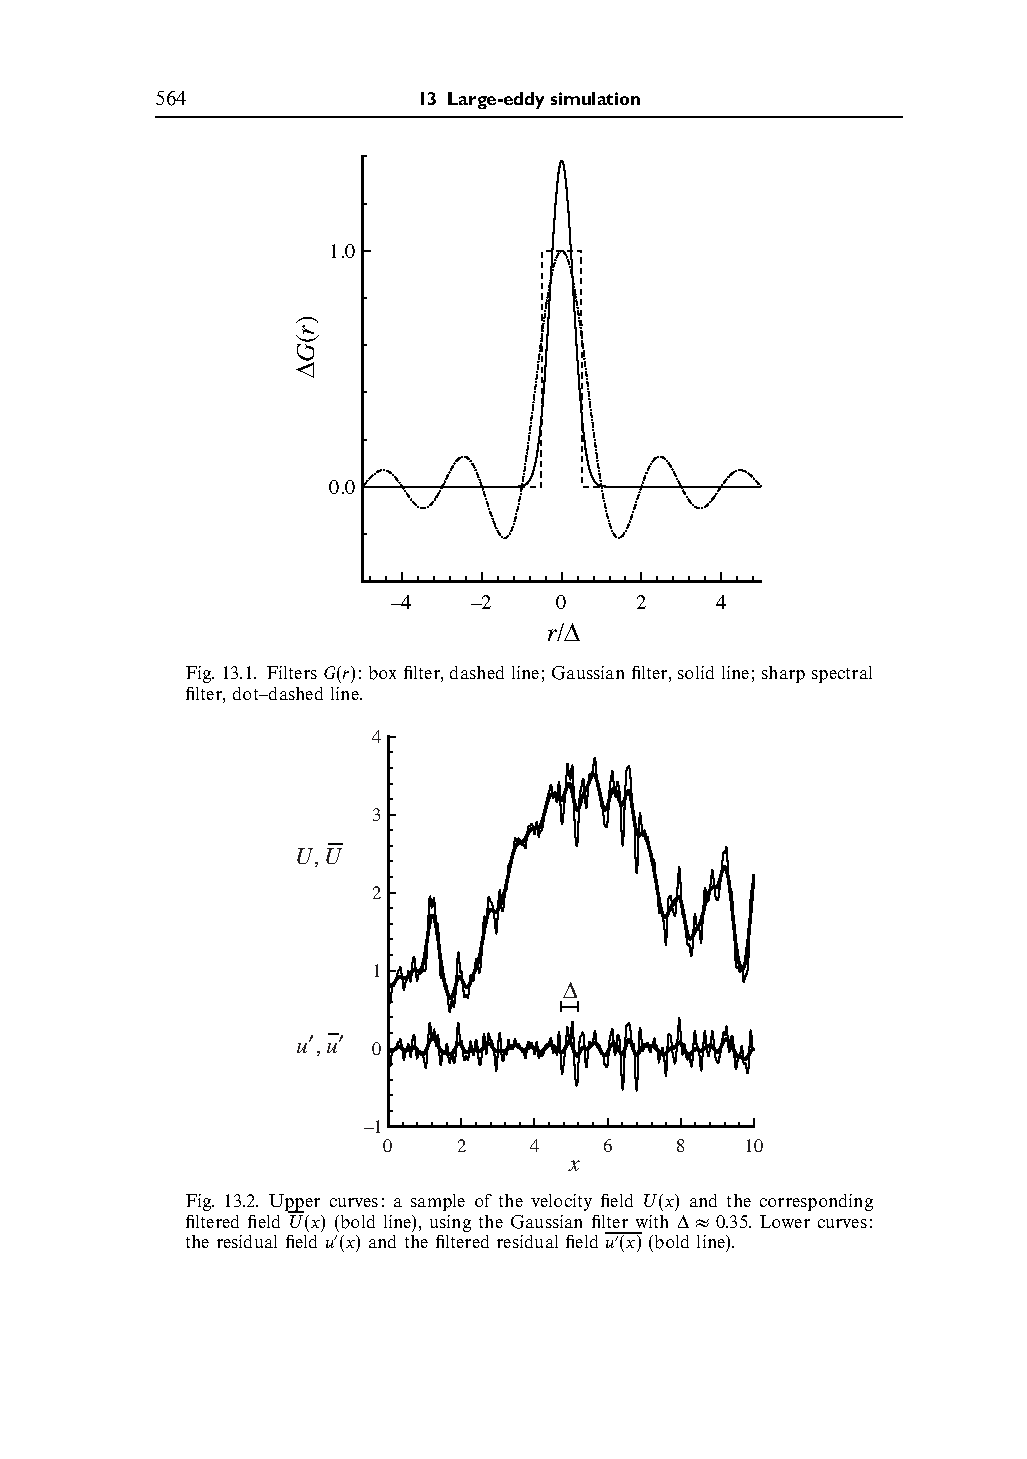
\includegraphics[width=0.6\linewidth,trim={4.8cm 4.8cm 2.8cm 12.1cm},clip]{Imagenes/03/les}
	\caption{Curva superior: una muestra de un campo de velocidad $u$ y su correspondiente campo filtrado $\overline{u}$ (en negrita). Curva inferior: campo residual $u'$ y campo residual filtrado $\overline{u'}$ (en negrita). Fuente: Pope (2000) \cite{pope2000turbulent}.}
	\label{fig:03_les}
\end{figure}

Se debe tener en cuenta que el filtro es en el fondo un nuevo operador matemático que cumple sus propias propiedades y que permite separar las escalas grandes de las pequeñas. Para una mejor descripción teórica de lo que implica un operador de filtrado se puede recurrir a Berselli et al. (2005) \cite{9783540263173}.

\subsection{Ecuaciones de Conservación Filtradas}
La aplicación del filtro a la ecuación de conservación de masa para flujo incompresible, da como resultado el hecho de que tanto el campo filtrado $\overline{u}$ como el campo residual $u'$ son solenoidales,
\be \partial_i \overline{u}_i = \partial_i u'_i = 0\ee
Utilizando esto, se escribe la ecuación de momemtum filtrada como:
\be
\partial_t \overline{u}_i + \partial_j(\overline{u_j u_i}) = \frac{1}{\rho} \partial_i \overline{p} + \nu\partial_{jj}\overline{u}_i
\ee
Se define el tensor de esfuerzos residuales como:
\be \tau_{ij}^R \equiv \overline{u_j u_i} - \overline{u}_j \overline{u}_i \ee
El cual es análogo al tensor de esfuerzos de Reynolds\footnote{Para diferenciar la notación, se utilizan corchetes para indicar promedio y $^*$ para indiciar fluctuaciones. De esta forma la descomposición de Reynolds se escribe $u_i = \langle u_i\rangle + u^*_i$}:
\be \langle u^*_i u^*_j \rangle = \langle u_i u_j \rangle - \langle u_i \rangle \langle u_j \rangle \ee
La energía cinética residual es:
\be k_r = \frac{1}{2}\tau_{ii}^R \ee
Y el tensor de esfuerzos residuales anisotrópicos se define como:
\be \tau_{ij}^r = \tau_{ij}^R - \frac{2}{3}k_r \delta_{ij} \ee
El segundo término de la ecuación anterior corresponde al esfuerzo residual isotrópico. Este se puede incluir dentro de la presión para reescribir la ecuación de momemtum como:
\be
\partial_t \overline{u}_i + \overline{u}_j \partial_j(\overline{u}_i) = \frac{1}{\rho} \partial_i \overline{p} + \nu\partial_{jj}\overline{u}_i - \partial_j \tau_{ij}^r
\ee

Para formar una ecuación de transporte para la energía cinética del campo filtrado primero se aplica el filtro a la energía cinética del campo total $E$ como:
\be \overline{E} = \frac{1}{2}\overline{u_i u_i} \ee
Esta puede ser descompuesta como:
\be \overline{E} = E_f + k_r \ee
donde $E_f=\frac{1}{2}\overline{u}_i\overline{u}_i$ es la energía cinética del campo filtrado y $k_t$ es la energía cinética residual.

Ahora, una contracción de la conservación de momemtum filtrada con $\overline{u}_i$ da la ecuación de transporte para $E_f$:
\be  
\partial_t E_f + \overline{u}_j\partial_j E_f + \frac{1}{\rho}\partial_i(\overline{u}_i\overline{p})+\partial_j(\overline{u}_i\tau_{ij}^r)-2\nu\partial_j(\overline{u}_i\overline{S}_{ij})= - \varepsilon_f -\Pi
\ee
Los términos al lado izquierdo corresponden a términos de transporte. Al lado derecho se ubican las fuentes o sumideros. $\varepsilon_f$ corresponde a la disipación viscosa por el campo de velocidad filtrado:
\be \varepsilon_f = 2\nu \overline{S}_{ij}\overline{S}_{ij} \ee
$\Pi$ es la tasa de producción de energía cinética residual (o disipación de submalla). Representa el traspaso de energía desde las escalas filtradas a las residuales y puede ser positivo o negativo (permitiendo \emph{backscatter}),
\be 
\Pi = -\tau_{ij}^r\overline{S}_{ij}
\ee 
\subsection{Modelación de los Esfuerzos Residuales}
Para lograr la clausura de las ecuaciones filtradas, se necesita un modelo para el esfuerzo residual anisotrópico $\tau_{ij}^r$. El modelo mas simple es el propuesto por Smagorinsky (1963), el cual también sirve como base para varios modelos mas avanzados.
\subsubsection{Modelo de Smagorinsky}
El modelo se puede ver en dos partes. Primero el modelo de viscosidad turbulenta lineal:
\be \tau_{ij}^r = -2\nu_t \overline{S}_{ij} \ee
se usa para relacionar el esfuerzo residual con la tasa de deformación filtrada. El coeficiente de proporcionalidad $\nu_t(x_i,t)$ es la viscosidad turbulenta de los movimientos residuales. 

Segundo, a través de una analogía con la hipótesis de largo de mezcla, la viscosidad turbulenta se modela como:
\be \nu_t = \ell_s^2 \overline{\mathcal{S}} \ee
\be \nu_t = (C_S \Delta)^2 \overline{\mathcal{S}} \ee
donde $\mathcal{S}$ es la tasa de deformación filtrada característica. $\ell_s$ es la escala de longitud de Smagorinsky, la cual, por medio de un coeficiente de Smagorinsky $C_s$($\sim 0,17$) se toma como proporcional al ancho del filtro $\Delta$.
\subsubsection{Modelo de Deardorff}
Tomando en consideración que el modelo de Smagorinsky es instantáneo y local, se torna natural el buscar incorporar los efectos no locales y de historia a través de alguna ecuación de transporte para $\tau_{ij}^r$. 

Deardorff (1974) planteó una ecuación de transporte para $k_r$\footnote{La estructura de la ecuación de transporte puede variar según el caso. Para motivos de esta tesis la forma de esta ecuación se verá en el próximo capítulo.} y logró la clausura a través de las siguientes relaciones:
\be \varepsilon_r = \frac{C_E k_r^{3/2}}{\Delta} \ee
\be \nu_t = C_v k_r^{1/2}\Delta \ee
Donde $C_E\approx 0.7$ y $C_v\approx 0.1$. $\varepsilon_r$ es la tasa de disipación de energía cinética residual. Modelos de este tipo son ampliamente usados en meteorología y es este el que se implementa en las simulaciones de esta tesis.
\newpage
\section{Asimilación de Datos}
La asimilación de datos (\emph{Data Assimilation}, en adelante DA) es un método de análisis con el cual información proveniente de observaciones es incorporado dentro de un modelo de estado. El modelo impone la consistencia dinámica sobre las variables y se encarga de esparcir la información espacialmente y sobre las variables.

Existen tres componentes en un proceso de asimilación de datos: las observaciones; el \emph{background}, que es la información sobre el estado de la atmósfera proveniente de algún modelo u otro análisis; y las restricciones dinámicas, que las impone el modelo.

Sea $\mathbf{x}$\footnote{Para esta sección se utilizará la negrita para indicar vectores y matrices.} el vector de estado de tamaño $n$ que define el estado de la atmósfera basado en algún modelo o análisis\footnote{La dimensión de $\mathbf{x}$ será igual a la cantidad de elementos en la malla multiplicado por la cantidad de variables de estado del modelo.} y sea $\mathbf{x}_t$ el vector que representa la mejor aproximación posible del estado de la atmósfera en la malla numérica\footnote{Notar que $\mathbf{x}_t$ no es el estado real instantáneo de la atmósfera debido a los errores de representación del modelo.}. El vector de \emph{background} $\mathbf{x}_b$, será la primera aproximación para $\mathbf{x}_t$. Si se denomina $\mathbf{x}_a$ al resultado del análisis, el problema se reduce entonces a hallar la corrección $\delta \mathbf{x}$ tal que,
\begin{equation*}
	\mathbf{x}_a = \mathbf{x}_b + \delta \mathbf{x}
\end{equation*}
sea lo mas cercano posible a $\mathbf{x}_t$.

Las observaciones utilizadas en el análisis se almacenan en el vector de observación $\mathbf{y}$. En el proceso de análisis este vector de observación debe ser comparado con un vector de estado. Como cada grado de libertad del vector de estado evidentemente no tendrá su correspondiente observación, es necesario llevar a cabo una transformación desde el espacio del modelo hacia el espacio de observación. Esta transformación se realiza a través del operador de observación $H(\mathbf{x})$\footnote{$H(x)$ es una matriz también, sin embargo, y solo para este caso, no se utiliza la negrita para diferenciarla del operador linealizado $\textbf{H}$ que se verá mas adelante}. Básicamente este operador interpola las variables de estado desde los puntos de la malla numérica a los puntos de observación a través de una interpolación adecuada (por ejemplo: lineal o cuadrática) . La diferencia
\begin{equation*}
	\mathbf{y}-H(\mathbf{x}_b)
\end{equation*}
se llama vector de innovación, y la diferencia
\begin{equation*}
\mathbf{y}-H(\mathbf{x}_a)
\end{equation*}
es el residual del análisis.

Usando esta notación, el problema se puede escribir como:
\begin{equation}\label{eq:03_dataassim1}
	\mathbf{x}_a = \mathbf{x}_b + \mathbf{K}(\mathbf{y} - H(\mathbf{x}_b))
\end{equation}
donde $\mathbf{K}$ es la matriz peso de la innovación que se debe encontrar.
\subsection{Análisis Variacional Tridimensional}

Si bien es posible hallar una solución teórica al problema multidimensional expresado en la ecuación \ref{eq:03_dataassim1}, generalmente es ineficiente y por lo tanto se adopta una metodología de minimización de funcion de costo o, análisis variacional.

Se puede demostrar \cite{warner2010numerical} que el problema variacional multidimensional busca minimizar una función de costo $J(\mathbf{x})$, que pondera los errores provenientes del modelo $J_b$ (\emph{background}) y de las observaciones $J_o$ de la forma:

\be 
J(x) = J_b + J_o = \frac{1}{2}(\textbf{x}-\textbf{x}_b)^T \textbf{B}^{-1}(\textbf{x}-\textbf{x}_b) + \frac{1}{2}(H(\textbf{x})-\textbf{y})^T \textbf{R}^{-1}(H(\textbf{x})-\textbf{y})
\ee 
Acá $\textbf{B}$ es la matriz de covarianzas de los errores del \emph{background} y $\textbf{R}$ es la matriz de covarianzas de los errores de las observaciones. La importancia y desarrollo de estas se explicarán mas adelante.

Teóricamente el problema variacional se soluciona hallando el gradiente de la función de costo e igualando a cero, es decir:
\be 
\nabla J(x) = \textbf{B}^{-1}(\textbf{x}-\textbf{x}_b)-H^T\textbf{R}^{-1}(\textbf{y}-H(\textbf{x}))=0
\ee
Despejando se puede tener una solución analítica de la forma:
\be \label{eq:03_dataassim}
\textbf{x}_a = \textbf{x}_b + \textbf{B}H^T(H\textbf{B}H^T+\textbf{R})^{-1}(\textbf{y}-H(\textbf{x}_b)) 
\ee
La ecuación anterior es fácil de entender si se identifican las matrices $H\textbf{B}H^T$ que es la proyección del error del background en el espacio de observacion y $\textbf{B}H^T$ que es la proyección del error del background en espacio de background-observación. De esta manera el análisis no es mas que una combinación de la ponderación de los errores aplicado al vector de innovación.

Utilizando la terminología de la sección anterior, se deriva que:
\be
\mathbf{K} = \textbf{B}H^{T}(H\textbf{B}H^T + \textbf{R})^{-1}
\ee 
Esta matriz $K$ de peso de la innovación, nuevamente, es computacionalmente intensiva calcularla para un gran número de observaciones, es por esto que en la práctica el problema variacional se resuelve usando algún método de minimización o algoritmo descendiente como el gradiente conjugado o métodos de cuasi-Newton.
\subsection{Matrices de Covarianzas $\textbf{B}$ y $\textbf{R}$}
Las matrices de covarianzas cumplen un rol fundamental en el proceso de análisis, ya que son ellas las que se encargan de ponderar correctamente los valores del \emph{background} y de las observaciones de manera realista. 

La matriz $\textbf{B}$ es la matriz de covarianzas de los errores del \emph{background}, sus dimensiones son de $n\times n$. La correcta estimación de esta matriz es muy importante para el proceso de análisis ya que  controla la influencia para el incremento del análisis en términos de la magnitud y de su forma. Con respecto a la forma, define el esparcimiento de la información desde una observación hasta la malla de análisis, y con respecto a la magnitud, si los errores del \emph{background} son grandes se le da un mayor peso a la observación.

Para un caso multi-dimensional:
\be 
\mathbf{B} = \overline{(\varepsilon_b - \overline{\varepsilon}_b)(\varepsilon_b - \overline{\varepsilon}_b)^T}
\ee 
Donde $\varepsilon$ es el vector de errores.
La matrix $\textbf{B}$ corresponde a una matriz cuadrada y simétrica con variazas a los largo de su diagonal. Por ejemplo, para un caso simple tridimensional:
\be 
\textbf{B} = \begin{pmatrix}
	\text{var}(e_1) & \text{cov}(e_1,e_2) & \text{cov}(e_1,e_3) \\
	\text{cov}(e_1,e_2) & \text{var}(e_2) & \text{cov}(e_2,e_3) \\
	\text{cov}(e_1,e_3) & \text{cov}(e_2,e_3) & \text{var}(e_3) \\
\end{pmatrix}
\ee 
Los términos fuera de la diagonal son las covarianzas cruzadas entre cada par de variables\footnote{Acá variable se usa en el sentido de cada variable dependiente en cada punto de malla} en el modelo. Hay tres maneras para estimar esta matriz:
\begin{enumerate*}
	\item[1.] \textbf{Covarianzas del error precalculadas:} Algunos métodos de asimilación de datos usan covarianzas precalculadas que pueden estar basadas en (a) un promedio de muchos estados distintos de la atmósfera, (b) consideraciones teóricas, o (c) simulaciones numéricas. Este último método es el que aplica el software WRF para hallar $\textbf{B}$.
	\item[2.] \textbf{Ponderación espacial anisotrópica no óptima:} Un ejemplo de esta metodología, por ejemplo, utiliza la información de la orografía para controlar la dispersión del vector de innovación a baja altura. La justificación de esto es que las covarianzas entre puntos que están en lados opuestos a una montaña deben ser pequeñas. De esta manera, la distribución del incremento de análisis es anisotrópica.
	\item[3.] \textbf{Covarianzas del error completamente régimen-dependiente:} Los métodos anteriores no toman en consideración los eventos diarios meteorológicos que se llevan a cabo en la atmósfera y que influyen fuertemente en la manera en la que las observaciones se analizan. Algunos métodos de asimilación de datos sofisticados, calculan las covarianzas del error del \emph{background} en función del flujo que evolucionan a través del proceso de asimilación.
\end{enumerate*}



Con respecto a la matriz $\textbf{R}$, esta es la matriz de convarianzas de los errores de las observaciones, sus dimensiones son de $p\times p$, donde $p$ es la cantidad de observaciones a analizar. Generalmente los errores de las observaciones son considerados independientes, especialmente cuando son realizadas por distintos instrumentos. Las varianzas generalmente son estimadas basadas en el conocimiento de las características de los instrumentos, los cuales pueden ser estudiados en el laboratorio. La mayoría de los modelos de $\textbf{R}$ son diagonales o casi diagonales.
%
\chapter{Weather Research and Forecast (WRF)}
\section{Aspectos Generales}
El software ARW-WRF (Advanced Research WRF) es un modelo atmosférico no hidrostático que resuelve las ecuaciones de Euler para flujo compresible en su forma conservativa y utilizando una coordenada vertical de masa (o de presión hidrostática). Su coordenada vertical se define como:
\begin{equation}\label{eq:04_eta}
\eta = \frac{p_{dh}-p_{dht}}{\mu_d}
\end{equation}
Donde $p_{dh}$ corresponde a la componente hidrostática de la presión del aire seco, y:
\begin{equation}
\mu_d = p_{dhs} - p_{dht}
\end{equation}
es el peso de la columna del aire seco en la superficie. En estas ecuaciones los subíndices $t$ y $s$ corresponden a los límites superior (top) e inferior (surface) del dominio. Un esquema de como se distribuye esta coordenada verticalmente y como sigue al terreno se puede ver en la Figura \ref{fig:04_eta}.

\begin{figure}[h!]
	\centering
	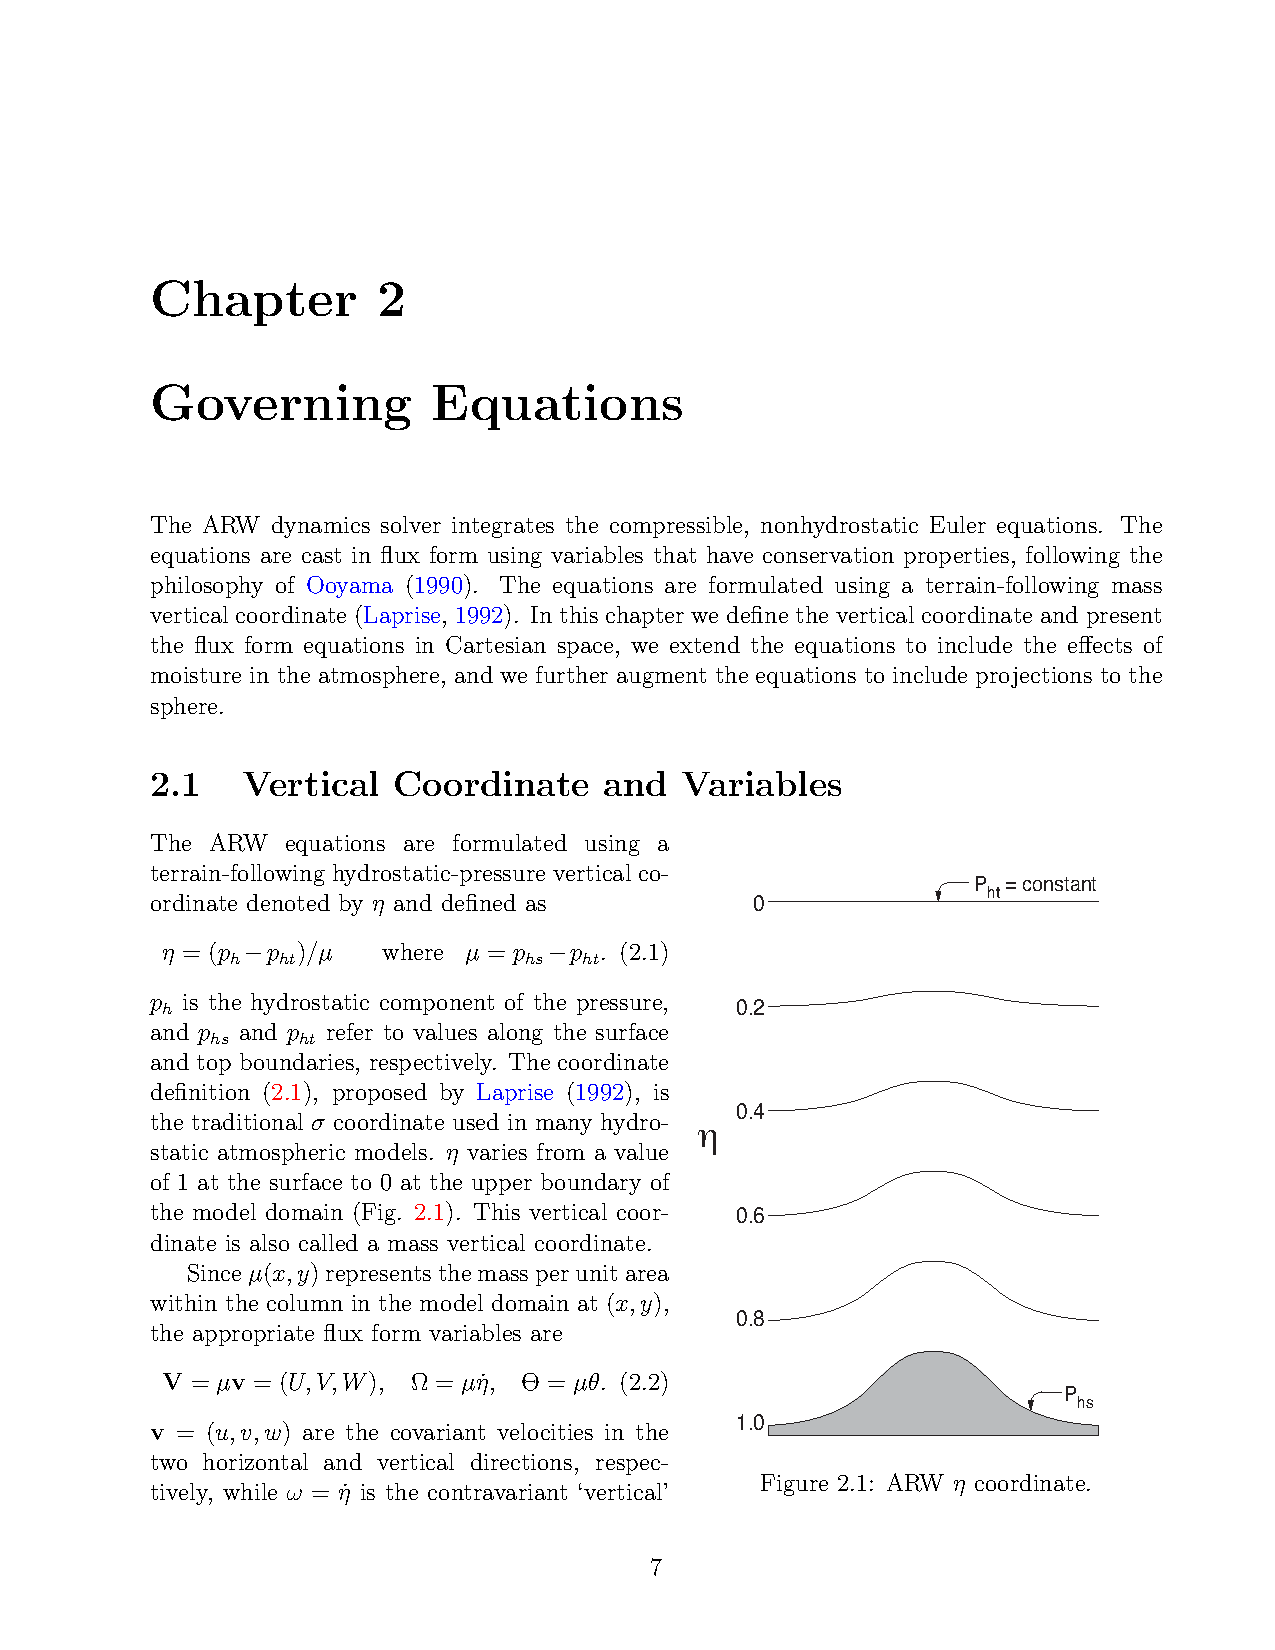
\includegraphics[width=0.55\linewidth,trim={11.5cm 3.3cm 1cm 14cm},clip]{Imagenes/04/eta}
	\caption{Estructura de la coordenada vertical.}
	\label{fig:04_eta}
\end{figure}

Las variables principales que resuelve WRF son las velocidades covariantes $(u,v,w)$, la masa de aire seco $\mu_d$, el geopotencial $\phi = gz$, la temperatura potencial $\theta$, la presión $p$, el inverso de la densidad $\alpha= 1/\rho$ y la energía cinética turbulenta $k$. 

El cambio de coordenadas que introduce la ecuación \ref{eq:04_eta} en las ecuaciones de Euler hace que aparezcan términos métricos y que la forma de escribir las ecuaciones sea diferente a lo acostumbrado a ver en mecánica de fluidos. El detalle de la transformación y el uso de $\mu_d$ en la ecuaciones se puede ver en la nota técnica del código \cite{https://doi.org/10.5065/d68s4mvh}.

A priori, las ecuaciones de momentum, temperatura potencial, energía cinética turbulenta y otros escalares relevantes tienen una forma acoplada con la masa de aire seco, de la forma:
\begin{equation}\label{eq:ec_conervacion}
\partial_t (\mu_d\theta) + \partial_x(\mu_d u \theta)+\partial_y(\mu_d v \theta)+\partial_\eta (\mu_d \omega \theta) = F
\end{equation}
Si bien $\theta$ es la temperatura potencial, esta ecuación es válida para cualquier otro escalar mencionado anteriormente.
$F$ es la suma de los forzamientos externos (es una ecuación de Euler), como puede ser la mezcla turbulenta o fuerzas de Coriolis. Además:
\begin{equation}
\omega = d_t\eta = \dot{\eta}
\end{equation}
es la velocidad en la coordenada vertical. Notar que la ecuación \ref{eq:ec_conervacion} corresponde a una ecuación de conservación de un escalar pasivo.

Para la discretización espacial del modelo se utiliza una malla de Arakawa tipo C con un tamaño de malla constante en las direcciones horizontales, pero variable en la vertical. Para la discretización temporal se utiliza un método explícito RK3 y un filtro que permite separar las ondas de alta frecuencia (ondas de presión y gravedad) de las ondas del espacio físico (o meteorológicamente relevantes). Las ondas de alta frecuencia son integradas en un paso de tiempo intermedio para asegurar estabilidad.

A continuación se presenta una lista con las principales características del modelo ARW-WRF en su versión 3:
\begin{itemize*}
	\item Ecuaciones no hidrostáticas completamente compresibles (con opción hidrostática)
	\item Aplicaciones globales y regionales
	\item Términos de curvatura y Coriolis completos
	\item Código portátil capaz de correr altamente en paralelo y en una gran variedad de sistemas operativos.
	\item Anidamiento de dos vías con múltiples nidos y niveles
	\item Anidamiento de una vía con refinamiento vertical
	\item Coordenada vertical basada en masa que sigue al terreno
	\item Espaciamiento vertical variable y ajustable
	\item Factores de escala para proyecciones cartográficas: Conformal, Lambert, Mercator, Lat-Lon
	\item Malla escalonada tipo Arakawa C
	\item Integración temporal con métodos RK de 2do o 3er orden
	\item Forma conservativa para las variables pronosticas
	\item Opciones de advección (horizontal y vertical) de 2do hasta 6to orden
	\item Opciones de transporte monótono y advección positiva para escalares
	\item Formulación para la turbulencia de submalla en el espacio coordenado y físico.
	\item Filtro de amortiguamiento para la divergencia
	\item Amortiguamiento de Rayleight y absorción en el borde superior
	\item Condiciones de borde laterales reales o ideales
	\item Opciones para físicas de: capa superficial, capa límite planetaria, radiación superficial y atmosférica, microfísicas y convección de cúmulos.
	\item Modelos oceánicos
	\item Anudamiento de datos a través asimilación de datos
	\item Inicialización con filtro digital
	\item Paso de tiempo adaptativo
	\item Ejemplos para casos idealizados
\end{itemize*}

El desarrollo del modelo WRF ha sido un esfuerzo colaborativo entre NCAR (\emph{National Center for Atmospheric Research}), NOAA (\emph{National Oceanic and Atmospheric Administration}), NCEP (\emph{National Centers for Environmental Prediction}), ESRL (\emph{Earth System Research Laboratory}), NRL (\emph{Naval Research Laboratory}), AFWA (\emph{Department of Defense's Air Force Weather Agency}), CAPS (\emph{Center for Analysis and Prediction of Storms}), la universidad de Oklahoma y el FAA (\emph{Federal Aviation Administration}) con el objetivo de crear un modelo de predicción mesoescala de última generación para avanzar en la comprensión y predicción del clima, junto con entregar una herramienta de acceso libre a toda la comunidad.

Junto con el núcleo dinámico (ARW), el software WRF viene con un sistema de preproceso (WPS) que se encarga de formar los dominios, asignar las bases de datos de orografía y uso de suelo e interpolar horizontalmente las condiciones iniciales y de borde que se utilizaran. También, WRF viene con un código de asimilación des dato nativo (WRFDA) el cual es el encargado de manipular los datos de observaciones en terreno, filtrarlos y efectuar la asimilación de datos.
 
\section{Ecuaciones Resueltas}
Tal como se mencionó en la sección anterior, las ecuaciones a resolver serán las ecuaciones de Euler, las cuales, a priori, tienen una forma como la de la ecuación demostrativa \ref{eq:ec_conervacion} en el sentido de que la suma de las aceleración local y la aceleración advectiva se va a balancear con distintos forzamientos externos.

Para construir el sistema de ecuaciones que utiliza el solver, se deben considerar las siguientes modificaciones:
\paragraph{Coordenada Vertical} La descripción del sistema en función de la masa de aire seco $\mu_d$ introduce las siguientes variables acopladas:
\begin{equation}
\vec{V}=\mu_d\vec{v}=(U,V,W)\quad;\quad \Omega = \mu_d \omega \quad;\quad \Theta = \mu_d \theta
\end{equation}
De esta manera los operadores con los cuales es posible escribir las ecuaciones en forma conservativa quedan:
\begin{equation}
\nabla\cdot\vec{V}a = \partial_x(Ua)+\partial_y(Va)+\partial_\eta (\Omega a)
\end{equation}
\begin{equation}
\vec{V}\cdot \nabla a = U\partial_x a + V\partial_y a + \Omega\partial_\eta a
\end{equation}
\paragraph{Inclusión de la Humedad} En vez de agregar términos fuentes a la ecuación de Euler, se trabaja considerando la conservación de masa del aire seco. Se agregan ecuaciones de conservación para las razones de mezcla $q_m=q_v,q_c,q_i,...$ que corresponden al vapor de agua, nubes, lluvia, hielo, etc. El valor de $\alpha$ para un elemento diferencial de aire se computa entonces como:
\begin{equation}
\alpha = \alpha_d(1+q_v+q_c+q_r+q_i+...)
\end{equation}
La ecuación de estado ahora comtempla la humedad de la forma:
\begin{equation}\label{eq:04_gasideal}
p = p_0\left(\frac{R_d \theta_m}{p_0 \alpha_d}\right)^\gamma
\end{equation}
Donde $R_d$ es la constante de gas ideal para el aire seco y $\gamma = c_p/c_v = 1.4$. Además,
\begin{equation}
\theta_m = \theta(1+(R_v/R_d)q_v)\approx\theta(1+0.61q_v)
\end{equation}
Es la temperatura potencial virtual.
\paragraph{Proyecciones Cartográficas} Para implementar las proyecciones cartográficas, el ARW utiliza factores de mapa $m_x,m_y$. Estos corresponden a la razón entre una distancia en el espacio computacional y la misma distancia en la superficie de la tierra:
\begin{equation}
(m_x,m_y) = \frac{(\Delta x, \Delta y)}{\text{distancia en la tierra}}
\end{equation}
De esta manera las variables de momentum quedan como:
\begin{equation}
U = \frac{\mu_d}{m_x}u\quad;\quad V = \frac{\mu_d}{m_y}v\quad;\quad W = \frac{\mu_d}{m_y}w\quad;\quad \Omega = \frac{\mu_d}{m_y}\dot{\eta}
\end{equation}
Si se utiliza una proyección isotrópica (Lambert conformal, Estereográfica polar, Mercator), los factores de mapa son idénticos: $m_x=m_y = m$.
\paragraph{Fuerza de Coriolis y Términos de Curvatura} Estos se agregan como forzamientos al lado derecho de la ecuación, tal como se muestra en la ecuación demostrativa \ref{eq:ec_conervacion}. Para el solver, estos toman la siguiente forma:
\begin{equation}
F_{U_{cor}} = \frac{m_x}{m_y}\left[ fV + \frac{uV}{r_e}\tan\psi \right] - \frac{uW}{r_e} - eW\cos\alpha_r
\end{equation}
\begin{equation}
F_{V_{cor}} = \frac{m_y}{m_x}\left[ -fU + \frac{uU}{r_e}\tan\psi - \frac{vW}{r_e} - eW\sin\alpha_r \right]
\end{equation}
\begin{equation}
F_{W_{cor}} = e\left( U\cos\alpha_r - (m_x/m_y)V\sin\alpha_r \right) + \left( \frac{uU + (m_x/m_y)vV}{r_e} \right)
\end{equation}
Donde $\alpha_r$ es el ángulo de rotación local entre el eje $y$ y los meridianos, $\psi$ es la latitud, $f=2\Omega_e\sin\psi, e=2\Omega_e\cos\psi$, $\Omega_e$ es la velocidad angular de la tierra y $r_e$ es el radio de la tierra.
\paragraph{Forma de Perturbación de las Ecuaciones Governantes} Finalmente, para disminuir los errores de truncatura, redondeo y otros problemas computacionales, se separan las variables de estado como la suma de una componente hidrostática (denotado por una barra) y una perturbación.
\begin{equation*}
p=\overline{p}(\overline{z}) + p';\quad \phi=\overline{\phi}(\overline{z}) + \phi';\quad \alpha=\overline{\alpha}_d(\overline{z}) + \alpha_d';\quad \mu_d=\overline{\mu}_d(x,y) + \mu_d'
\end{equation*}
De esta manera las ecuaciones \ref{eq:04_wrf1} -- \ref{eq:04_wrf2} son las que se utilizan en el solver.
\begin{equation}\begin{split}\label{eq:04_wrf1}
&\partial_t U + m_x[\partial_x(Uu)+\partial_y(Vu)]+\partial_\eta(\Omega u) \\
&+ (m_x/m_y)(\alpha/\alpha_d)[\mu_d(\partial_x\phi' + \alpha_d \partial_x p' + \alpha_d'\partial_x \overline p)+\partial_x\phi(\partial_\eta p' - \mu_d')] = F_U
\end{split}\end{equation}
\begin{equation}\begin{split}
&\partial_t V + m_y[\partial_x(Uv)+\partial_y(Vv)]+(m_y/m_x)\partial_\eta(\Omega v) \\
&+ (m_y/m_x)(\alpha/\alpha_d)[\mu_d(\partial_y\phi' + \alpha_d \partial_y p' + \alpha_d'\partial_y \overline p)+\partial_y\phi(\partial_\eta p' - \mu_d')] = F_V
\end{split}\end{equation}
\begin{equation}\begin{split}
\partial_t W + m_x[\partial_x(&Uw)+\partial_y(Vw)]+\partial_\eta(\Omega w) \\
\hspace{1cm}&- m_y^{-1}g(\alpha/\alpha_d)[\partial_\eta p' - \overline{\mu}_d(q_v+q_c+q_r)]+m_y^{-1}\mu_d' g = F_W
\end{split}\end{equation}
\begin{equation}\begin{split}
\partial_t \mu_d' + m_x m_y[\partial_x U + \partial_y V] + m_y\partial_\eta \Omega = 0
\end{split}\end{equation}
\begin{equation}\begin{split}
\partial_t \phi' + \mu_d^{-1}[m_x m_y(U\partial_x\phi + V\partial_y\phi) + m_y \Omega \partial_\eta\phi - m_ygW] = 0
\end{split}\end{equation}
\begin{equation}\begin{split}\label{eq:04_wrf2}
\partial_t \Theta + m_x m_y [\partial_x(U\theta)+\partial_y(V\theta)]+m_y\partial_\eta(\Omega \theta) = F_\Theta
\end{split}\end{equation}
Donde las primeras tres ecuaciones corresponden a la conservación de momentum, la cuarta a la conservación de masa, la quinta es la derivada material de la deficinión del geopotencial y la sexta es la ecuación de transporte para la temperatura potencial (o cualquier otro escalar relevante como las fracciones de mezcla de las fases del agua).

El sistema se cierra incorporando las ecuaciones diagnósticas para el geopotencial (en su forma de perturbación) y para la presión (gas ideal, ecuación \ref{eq:04_gasideal}):
\begin{equation}
\partial_\eta \phi ' = -\overline{\mu}_d \alpha_d' - \alpha_d \mu_d'
\end{equation}

\section{Aspectos Numéricos Relevantes}
A continuación se presentan en detalle aquellos aspectos del código que son fundamentales para el entendimiento y el desarrollo de los experimentos realizados. Algunos temas, como por ejemplo el tratamiento de la advección, la aplicación de ciertos filtros para amortiguar ondas o el detalle de la integración temporal para los modos físicos y acústicos, fueron dejados voluntariamente de lado en beneficio de la extensión de este trabajo. Se recomienda al lector revisar la nota técnica del código \cite{https://doi.org/10.5065/d68s4mvh} si desea tener un conocimiento extensivo con respecto al funcionamiento total del WRF.
\subsection{Difusión}
La difusión y los flujos turbulentos en el espacio físico $(x,y,z)$ se calculan haciendo uso de la métrica del espacio a partir de la ecuación para el geopotencial $\phi$:
\begin{eqnarray}
z_x=g^{-1}\delta_x\phi \\
z_y=g^{-1}\delta_y\phi
\end{eqnarray}
Donde $\delta_{x,y}$ es el operador discreto para la derivada, es decir:
\begin{equation}
\delta_x a = \frac{a_{i+1/2}-a_{i-1/2}}{\Delta x}
\end{equation}
El término difusivo se agrega al lado derecho de las ecuaciones de Euler, junto al resto de las fuerzas externas. Estas se ven:
\begin{eqnarray}
\partial_t U = \ldots - m_x[\partial_x\tau_{11}+\partial_y\tau_{12}-\partial_z(z_x\tau_{11}+z_y\tau_{12})]-\partial_z\tau_{13} \\
\partial_t V = \ldots - m_y[\partial_x\tau_{12}+\partial_y\tau_{22}-\partial_z(z_x\tau_{12}+z_y\tau_{22})]-\partial_z\tau_{23} \\
\partial_t W = \ldots - m_y[\partial_x\tau_{13}+\partial_y\tau_{23}-\partial_z(z_x\tau_{13}+z_y\tau_{23})]-\partial_z\tau_{33}
\end{eqnarray}
Y el tensor de esfuerzos viscosos es:
\begin{equation}
\tau_{ij} = -\mu_d K_{h,v}S_{ij}
\end{equation}
donde $K_{h,v}$ es la viscosidad turbulenta en dirección horizontal o vertical según corresponda y $S_{ij}$ es el tensor tasa de deformación que bajo esta formulación toma la siguiente forma:
\begin{align}
S_{11} &= 2m_xm_y[\partial_x(m_y^{-1}u)-z_x\partial_z(m_y^{-1}u)]  \\
S_{22} &= 2m_xm_y[\partial_y(m_x^{-1}v)-z_y\partial_z(m_x^{-1}v)]  \\
S_{33} &= 2\partial_z w  \\
S_{12} &= m_xm_y[\partial_y(m_y^{-1}u)-z_y\partial_z(m_y^{-1}u)+\partial_x(m_x^{-1}v)-z_x\partial_z(m_x^{-1}v)]  \\
S_{13} &= m_xm_y[\partial_x(m_y^{-1}w)-z_x\partial_z(m_y^{-1}w)]+\partial_z u  \\
S_{23} &= m_xm_y[\partial_y(m_y^{-1}w)-z_y\partial_z(m_y^{-1}w)]+\partial_z v  \\%
\end{align}

Por otro lado, la difusión de un escalar cualquiera $a$ es:
\begin{equation}\begin{split}
\partial_t(\mu_d a) = ... &+ [m_x(\partial_x-\partial_z z_x)(\mu_d m_x K_h(\partial_x - z_x\partial_z)) \\
&+m_y(\partial_y-\partial_z z_y)(\mu_d m_y K_h(\partial_y-z_y\partial_z))+\partial_z\mu_dK_v\partial_z]a
\end{split}\end{equation}

\subsubsection{Cálculo de la Viscosidad Turbulenta}
La opción por defecto para el modelo (simulaciones de mesoescala sin LES), es computar la viscosidad turbulenta horizontal $K_h$ por medio de la deformación horizontal usando un esquema de Smagorinsky de primer orden,
\begin{equation}
K_h = C_s^2 l^2[0.25(D_{11}-D_{22})^2+D_{12}]^{0.5}
\end{equation}
Con $C_s=0.25$ y $l=\sqrt{\Delta x\Delta y}$. La viscosidad turbulenta vertical $K_v$ queda definida según el esquema de parametrización utilizado para la capa límite planetaria.

Para las simulaciones de microescala utilizando LES la viscosidad turbulenta se calcula en función de la energía cinética turbulenta $k$ de la forma:
\begin{equation}
K_{h,v}=C_k l_{h,v}\sqrt{k}
\end{equation}
donde $C_k$ es una constante (normalmente $0.15<C_k<0.25$) y $l$ es un largo característico que se calcula en función de la isotropía de la malla, la resolución, $k$ y la estratificación de la forma:
\begin{align}
	l_v &= \min[\Delta z, 0.76\sqrt{k}/N]\quad&;&\quad N^2>0\\
	l_h &= \Delta z\quad&;&\quad N^2\leq 0
\end{align}
$N$ es la frecuencia de Brunt-Väisälä calculada para aire húmedo.

La clausura del modelo de turbulencia se hace considerando la ecuación de transporte para $k$ como:
\begin{equation}
\partial_t(\mu_d k) + (\nabla\cdot\vec{V}k)_\eta = \mu_d(\mathcal{P} + \mathcal{F} + \mathcal{D})
\end{equation}
Los términos al lado derecho corresponden a la producción de energía cinética turbulenta, a la flotación y a la disipación respectivamente. Estos se calculan como:
\begin{align}
	\mathcal{P}&= K_h (S_{11}^2 + S_{22}^2 + S_{12}^2) + K_v (S_{33}^2 + S_{13}^2 + S_{23}^2)\\
	\mathcal{F}&=-K_v N^2\\
	\mathcal{D}&=-\frac{C k^{3/2}}{l_k}
\end{align}
Con las siguientes constantes:
\begin{align}
	C &= 1.9C_k + \frac{(0.93 - 1.9 C_k)l_k}{(\Delta x \Delta y \Delta z)^{1/3}}\\
	l_k &= \min[(\Delta x \Delta y \Delta z)^{1/3}, 0.76\sqrt{e}/N]
\end{align}
Queda entonces cerrado el problema de la turbulencia.
\subsection{Parametrizaciones Físicas}
Junto con el esquema para la difusión, el modelo ARW presenta otros esquemas disponibles para representar diversas físicas que ocurren dentro de la atmósfera. Estos esquemas generalmente se presentan como \emph{drivers} independientes del código principal y por lo tanto son usados como librerías para actualizar las tendencias de las variables de estado que modelan las ecuaciones de Euler. Las categorías de las físicas parametrizadas son: (1) Microfísicas, (2) Capa Límite Atmosférica, (3) Modelo de suelo-superficie, (4) Cúmulos y (5) Radiación.

A continuación se explicará brevemente la importancia dentro de la simulación de cada una, sin recurrir a desarrollos matemáticos extensos, debido a que WRF ofrece una gran variedad de opciones para cada una de las físicas.
\subsubsection{Microfísicas}
Se encarga de resolver explícitamente el vapor de agua, nubosidad y procesos de precipitación. También incluye procesos de sedimentación y el ajuste a la saturación. La diferencia entre los distintos modelos recae en la cantidad de variables a solucionar y el tipo de variables. Los modelos mas sofisticados pueden modelar 10 variables, incluyendo procesos de formación de hielo y variables con mezcla de fases.
\subsubsection{Parametrización de Cúmulos}
Son responsables de modelar el efecto de submalla de las nubes convectivas. En específico busca representar los flujos verticales debido a las escalas no resueltas y compensar el movimiento fuera de las nubes. Opera sobre toda una columna de aire y entrega el calentamiento vertical y perfiles de humedad. Los modelos mas avanzados pueden entregar los campos de tendencias para nubes y precipitacion.

Teóricamente, esta parametrización debe usarse solo para malla gruesas (>10 [km]) cuando es necesario representar el movimiento que no pudo ser resuelto. Mallas mas finas pueden resolver explícitamente los vórtices verticales y por lo tanto no debe usarse.
\subsubsection{Capa Superficial}
Los esquemas de capa superficial se encargan de calcular la velocidad de fricción $u^*$ y los coeficientes de mezcla que permiten el cálculo de los flujos de calor y humedad desde la superficie por el esquema de modelo de suelo y los esfuerzos de pared por el esquema de capa límite. Generalmente cada modelo de capa superficial tiene su modelo de capa límite asociado, sin embargo, se espera que en el futuro estos puedan independizarse. La manera de hallar los coeficientes se hace a través del uso de funciones de estabilidad o por teorías de similaridad como aquella propuesta por Monin-Obukhov.
\subsubsection{Modelo de Suelo}
A través de los resultados obtenidos por los modelos de capa superficial, microfísicas, cúmulos y radiación, junto con los datos sobre el uso de suelo del terreno, el modelo de suelo se encarga de calcular los flujos de calor y humedad desde el suelo hacia la atmósfera. Estos flujos proveen las condiciones de borde inferior para el transporte vertical hecho por el modelo de capa límite. Los modelos de suelo poseen un amplio espectro de sofisticación, pudiendo manejar flujos térmicos y de humedad en numerosas capas de la tierra, junto con vegetación, raices, covertura de nieve, etc. Este modelo no modifica las tendencias de las variables de estado, sino que actualiza las condiciones del suelo.
\subsubsection{Capa Límite Planetaria}
Se encarga de entregar los flujos verticales de submalla ($K_v$) debido al transporte turbulento para toda la columna de aire, no solo la capa límite y de esta manera actualiza las tendencias de temperatura, humedad y momentum horizontal para el modelo. La mayoría de los modelos considera mezcla seca para la capa límite, pero existen modelos mas avanzados que pueden manejar efectos de saturación para la estabilidad vertical. Este esquema es unidimensional y asume que existe una clara separación entre los vórtices de submalla y los vórtices resueltos (i.e. fuera de la zona gris de la turbulencia). A medida que la resolución de la malla va aumentando hasta el tamaño de los metros, es mejor no utilizar un modelo de capa límite y calcular explícitamente la mezca vertical a través de un modelo 3D para la turbulencia (modo LES).
\subsubsection{Radiación Atmosférica}
Se encarga de calcular el calentamiento de la atmósfera debido a la divergencia del flujo radiativo y a la radiación de onda corta y onda larga desde la superficie. La radiación de onda larga incluye la radiación infraroja o térmica absorbida y emitida por los gases y superficies, además del flujo radiativo emitido por la superficie. La radiación de onda corta incluye la radiación emitida por el sol dentro del espectro visible, si bien la única fuente de onda corta es el sol, estos procesos incluyen la absorción, reflexión, y dispersión de las ondas en la atmósfera y superficies.
\section{Sistema de Asimilación de Datos WRFDA}
Tal como se explicó en el marco teórico, la función que se busca minimizar es la siguiente:
\begin{equation}
J(x) = \frac{1}{2}(\mathbf{x}-\mathbf{x_b})^T\mathbf{B}^{-1}(\mathbf{x}-\mathbf{x_b}) + \frac{1}{2}(\mathbf{y}-H(\mathbf{x}))^T \mathbf{R}^{-1}(\mathbf{y}-H(\mathbf{x}))
\end{equation}
WRF efectua esto a través de una formulación incremental del problema. Linealizando, sea $\delta \mathbf{x}=\mathbf{x} - \mathbf{x}_g$ y $\delta \mathbf{x}_g=\mathbf{x}_b - \mathbf{x}_g$ se tiene:
\begin{equation}
	J(\delta \mathbf{x}) = \frac{1}{2}(\delta \mathbf{x}- \delta \mathbf{x}_g)^T\mathbf{B}^{-1}(\delta \mathbf{x} - \delta \mathbf{x}_g) + \frac{1}{2}[H(\delta \mathbf{x} + \mathbf{x}_g)-\mathbf{y}]^T \mathbf{R}^{-1}[H(\delta \mathbf{x} + \mathbf{x}_g)-\mathbf{y}]
\end{equation}
Luego, se hace una serie de Taylor para el término de las observaciones:
\begin{equation}
J(\delta \mathbf{x}) = \frac{1}{2}(\delta \mathbf{x}- \delta \mathbf{x}_g)^T\mathbf{B}^{-1}(\delta \mathbf{x} - \delta \mathbf{x}_g) + \frac{1}{2}(\mathbf{H} \delta \mathbf{x} -\textbf{d})^T \mathbf{R}^{-1}(\mathbf{H}\delta \mathbf{x} -\textbf{d})
\end{equation}
Donde $d=y-H(\textbf{x}_g )$ y $\textbf{H}$ es la versión linealizada de $H$ es las cercanías de $\textbf{x}_g$.

En esta formulación $\textbf{x}_g$ es el primer estimador de la solución. Para la primera iteración $\textbf{x}_b=\textbf{x}_g$, pero en las iteraciones siguientes $\textbf{x}_g$ será el análisis del ciclo anterior $\textbf{x}_a$.

Para evitar el cálculo de la inversa de la matriz $\textbf{B}$ (que es grande), se hace el siguiente cambio de variable a la variable de control $\textbf{v}$:
\begin{equation}
	\delta \mathbf{x}=\textbf{U}\textbf{v}\quad;\quad \delta \mathbf{x}_g=\textbf{U}\textbf{v}_g 
\end{equation}
Donde $\textbf{U}$ es la raiz cuadrada de $\textbf{B}$ (en el sentido matricial), es decir:
\begin{equation}
\textbf{B}=\textbf{B}^{1/2}\textbf{B}^{T/2} = \textbf{U}\textbf{U}^{T}
\end{equation}
o,
\begin{equation}
\textbf{U}=\textbf{B}^{1/2}
\end{equation}
De la misma forma,
\begin{equation}
\textbf{B}^{-1} = \textbf{U}^{-T}\textbf{U}^{-1}
\end{equation}
La función de costo con respecto a la variable de control $\textbf{v}$ se vuelve:
\begin{equation}
J(\mathbf{v}) = \frac{1}{2}(\mathbf{v}- \mathbf{v}_g)^T(\mathbf{v} - \mathbf{v}_g) + \frac{1}{2}(\mathbf{H} \mathbf{U}\mathbf{v} -\textbf{d})^T \mathbf{R}^{-1}(\mathbf{H}\mathbf{U}\mathbf{v} -\textbf{d})
\end{equation}
\subsection{Modelación de $\textbf{B}$}
Tal como se habló en el capítulo del marco teórico, la matriz de covarianzas del error del \emph{background} $\textbf{B}$ es la encargada de (a) ponderar correctamente el valor del \emph{background} al análisis, y (b) esparcir la información espacialmente y a través de todas las variables. WRF posee su propio mecanismo de generación de la matriz $\textbf{B}$ utilizando el llamado método NMC \cite{https://doi.org/10.5065/d68s4mvh}.

Algunas propiedades relevantes de la matriz son:
\begin{itemize*}
	\item $\textbf{B}$ es cuadrada y simétrica.
	\item $\textbf{B}$ es una matriz semidefinida positiva, sus valores propios son positivos. 
\end{itemize*}

El en WRF esta matriz se forma a través de tres transformaciones secuenciales de la forma:
\be 
\textbf{B}=\textbf{U}_p \textbf{U}_v \textbf{U}_h \textbf{U}_p^T \textbf{U}_v^T \textbf{U}_h^T 
\ee
Donde $\textbf{U}_h$ es la transformación horizontal a través de filtros recursivos para modelar la correlación horizontal de las variables de control, $\textbf{U}_v$ es la transformación vertical a través de una descomposición en funciones ortogonales de la varianza vertical y $\textbf{U}_p$ es la transformación de balance/física a través de regresiones lineales con la función de corriente.
%
\chapter{Metodología}
\section{Alcance de la Investigación}

\section{Datos de entrada al modelo}
\subsection{Bases de datos utilizadas}
\subsubsection{Información Geográfica}
La información estática que sirve como condición de borde inferior al modelo debe extraerse de datos satelitales u otros similares con el objetivo que sea uniforme y confiable. Esta información debe ser siempre georeferenciada (protocolo GIS).

WRF utiliza una base de datos estática lo suficientemente amplia como para poder satisfacer un uso normal del modelo, sin embargo, si se desea utilizar WRF en condiciones extremas, es decir, a escalas lo suficientemente pequeñas como para que las bases de datos no satisfagan la resolución, es necesario actualizar algunas bases de datos. La información a actualizar debe ser:
\begin{itemize*}
	\item Altura del Terreno: Para una obtención precisa de los niveles $\eta$ en cada punto del dominio y por lo tanto una correcta representación del terreno complejo que va a ser el principal motivador de la turbulencia.
	\item Uso de Suelo: Posee la información acerca del \% de vegetación, coeficiente térmico superficial y, lo más importante, el coeficiente de rugosidad ($z_0$), que es el parámetro a utilizar para estimar los flujos superficiales.
\end{itemize*}
Las bases de datos a utilizar en las simulaciones serán:
\begin{itemize*}
	\item GMTED2010: Dataset por defecto del WRF para la altura del terreno. Obtenida el año 2010 por la USGS y la NGA con una resolución de 30'.
	\item ASTER: Es el único instrumento de alta resolución de la NASA ubicado en la plataforma Terra. Esta base de datos se hizo pública el año 2011 y entrega información de la altura del terreno con una resolución de 1' ($\approx 30$ [m]).
	\item MODIS: Información obtenida por lo satélites de la nasa. Entregan información en 20 categorías a una resolución de 15' de arco.
	\item Corine: Obtenida el año 2012 (proyecto CLC12) a través de imágenes satelitales con 100m de resolución para toda Europa. Posee 44 categorías y es la base de datos de uso de suelo abierta de más alta resolución existente hasta ahora. Para este trabajo se usa la versión 18.5 modificada del año 2016.
	\item Bolund: Los autores del experimento de Bolund entregan bases de datos de la orografía del terreno y el coeficiente de rugosidad para este con una resolución de 25 [cm]
\end{itemize*}
\subsubsection{Incorporación a WRF}
La manera en la que los datos descritos anteriormente son entregados, muchas veces no están en el formato en el que el preprocesador del modelo WRF (WPS) puede asimilarlo. Sin embargo, debido a los estándar exigidos para información georeferenciada, es posible manipularla de tal manera que puedan incorporarse al modelo. A continuación se describen algunos trabajos que debieron hacerse con las bases de datos.
\begin{enumerate*}
	\item ASTER: Cambio de formato de GeoTiff a binario.
	\item Bolund Oro.: La información entregada por el experimento Bolund viene dada en un datúm UTM Z32, por lo cuál se debe transformar a WSG84, además, debido a la lectura de la información, los autores trasladaron las coordenadas, por lo cual hubo que invertir esta traslación. Se debió transformar la altura del agua entregada (los autores por motivos de interpolación de mareas declaran un $z=0.75$ para agua) a un nivel de $z=0$, para un correcto uso del modelo. 
	\item Corine: Se debió transformar su datúm nativo de ETRS89 a WSG84 Debido a que la clasificación de suelo por Corine no está implementada en WRF, se debe hacer un remapeo de los índices al formato USGS. Este procedimiento está descrito en Pineta et. al. (2004). Por otra parte, la resolución de los datos CLC12 son bastante gruesos en comparación con los entregados por ASTER 1s, luego el WPS presentó algunos errores en reconocer las masas de tierra y para solucionar esto se procedió a hacer una afinación manual de los datos CLC12 en las zonas relevantes para la simulación. Esta afinación puede verse en las figuras anexas a este informe.
	\item Bolund LU: Los autores del experimento entregan información acerca del $z_0$ en el dominio de Bolund y en el mismo formato en el que entregan la orografía, por lo tanto se debieron hacer las mismas trasformaciones detalladas anteriormente y luego hacer calzar la información entregada con un índice de tipo de suelo y que además fuera consistente con las bases de datos de uso de suelo usadas en los dominios mas grandes.
\end{enumerate*}
\subsubsection{Condiciones Iniciales y de Borde del Modelo}
Para inicializar el modelo y para proveer de información en los contornos cada 6 horas, se utilizan los datos de los análisis operacionales provenientes del modelo global GFS con resolución de $0.5^\circ$ ($\approx 55.6$ [km])

Por otra parte, como el dominio mas grande a simular cae dentro de lo que es una simulación de mesoescala y tomando en consideración las proyecciones debido a la curvatura de la tierra para esta zona en particular, se decide fijar la condición de borde superior para la coordenada vertical de presión a $p_{dht} = 5000$ [kPa] siguiendo la recomendación del manual del programa.

La condición de borde inferior queda determinada por la información obtenida en los datos de uso de suelo para cada punto de la malla.
\section{Preproceso de la Asimilación de Datos}

\section{Posproceso de los datos}
\subsection{Interpolación de alturas}
ley logaritmica.
\subsection{Cálculo de Errores}
Considerando que el resultado final de las simulaciones realizadas es un archivo de texto con la serie de tiempo para los valores de $u,v$ y $w$ para cada punto de interés en el dominio, es necesario definir una estimación del error entre la simulación realizada y la serie de tiempo medida en el mástil.

Se decide utilizar dos indicadores para llevar a cabo esta tarea: el MAE y el RMSE.

El MAE (\emph{Mean Absolute Error}) entre dos variables continuas se calcula de la siguiente forma:

\be 
MAE = \frac{1}{n}\sum_{i=1}^n |y_i-x_i|
\ee

Es un promedio del valor absoluto de los errores.

Si graficáramos la correspondencia de los datos en un gráfico de $x$ vs $y$, el MAE correspondería al valor medio de la distancia horizontal entre cada punto y la línea $x=y$.

El RMSE (\emph{Root Mean Squared Error}) por otro lado se calcula como:

\be 
RMSE = \sqrt{\frac{1}{n}\sum_{i=1}^n (y_i-x_i)^2}
\ee

Y corresponde a la raíz de los momentos muestrales de segundo orden de la diferencia entre los valores a comparar, en otras palabras, es un análogo al MAE pero pondera con mayor importancia los errores mas grandes. Es un promedio de los errores al cuadrado.
\section{Caso de Validación: Terreno Plano Høvsøre}
\subsection{Aspectos generales de las simulaciones}

\begin{table}[h!]
	\caption{Dominio numerico espacial y temporal para simulación del caso Høvsøre.}\label{tab:exp}
	\centering\footnotesize
	\begin{tabular}{lcc}
		\toprule
		Parámetro & Selección \\
		\midrule
		Fecha	 	 & 2010-09-08   \\
		Hora Inicio	 	 & 06:00:00   \\
		Hora Término	 		 & 20:00:00  \\
		Puntos Malla Vert.	 	 & 47   \\
		$P_{top}$ 	& 5000 kPa\\
		\# Dominios	& 7   \\
		Lat. Centro	& 56.447984   \\
		Lon. Centro	& 8.151570   \\
		\bottomrule
	\end{tabular}
\end{table}

\begin{table}[h!]
	\caption{Valores característicos de cada dominio.}\label{tab:param_fis}
	\centering\footnotesize
	\begin{tabular}{llllllll}
		\toprule
		Dominio 				& d01	&	d02	&	d03	&	d04	&	d05	&	d06 &	d07 \\
		\midrule
		$N_x$		& 107 & 107 & 107 &107&107&107&107  \\
		$N_y$	 		& 107 & 107 & 107 &107&107&107&107  \\
		$\Delta x = \Delta y$	[m]	 		& 30000 & 10000 & 3333.3 &1111.1&222.22&74.074&24.691  \\
		$\Delta t$	[s]	 		& 90 & 30 & 10 &3.333&0.666&0.222&0.074  \\
		Orografía		 	& GMTED2010 & GMTED2010 & GMTED2010 &ASTER&ASTER&ASTER&ASTER  \\
		Uso de Suelo					& USGS & USGS & USGS &CLC12&CLC12&CLC12&CLC12 \\
		\bottomrule
	\end{tabular}
\end{table}

\begin{table}[h!]
	\caption{Parametrizaciones físicas utilizadas en el modelo.}\label{tab:param_fis}
	\centering\footnotesize
	\begin{tabular}{llllllll}
		\toprule
		Dominio 				& d01	&	d02	&	d03	&	d04	&	d05	&	d06 &	d07 \\
		\midrule
		Micro-físicas		 	& WSM5 & WSM5 & WSM5 &WSM5&WSM5&WSM5&WSM5  \\
		Cúmulos			 		& Grell & Grell & -- & -- & -- & -- & -- \\ 
		Capa Superficial	 	& MM5 & MM5 & MM5 & MM5 & MM5 & MM5 & MM5 \\
		PBL				 		& YSU & YSU & YSU & YSU & -- & -- & -- \\
		Modelo LES				 		& -- & -- & -- & -- & 1.5TKE & 1.5TKE & 1.5TKE \\
		Modelo de Suelo 		& Difus. & Difus. & Difus. & Difus. & Difus. & Difus. & Difus. \\
		Rad. Onda Larga	& RRTM &RRTM&RRTM&RRTM&RRTM&RRTM&RRTM \\
		Rad. Onda Corta	& Dudhia &Dudhia&Dudhia&Dudhia&Dudhia&Dudhia&Dudhia \\
		\bottomrule
	\end{tabular}
\end{table}

\begin{figure}[H]
	\centering
	\includegraphics[width=0.6\linewidth,page=1,trim={5mm 3mm 3mm 3mm},clip,frame]{Imagenes/05/hov_dom1_edit.jpg}%
	
	\bigskip%
	
	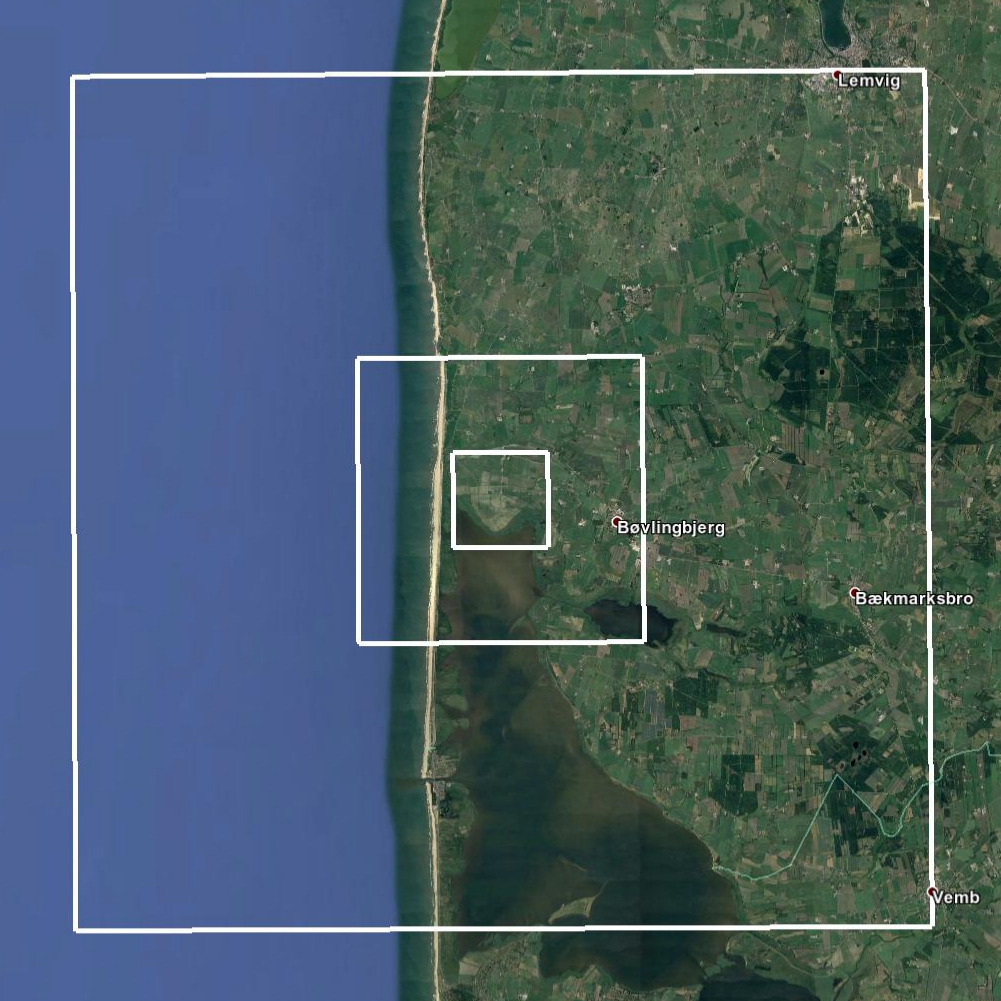
\includegraphics[width=0.6\linewidth,page=1,trim={5mm 3mm 3mm 3mm},clip,frame]{Imagenes/05/hov_dom2_edit.jpg}%
	\caption{Distribución telescópica de los 7 mallas anidadas en el dominio numérico.}
	\label{fig:dom_telesco}
\end{figure}

\begin{figure}[H]
	\centering
	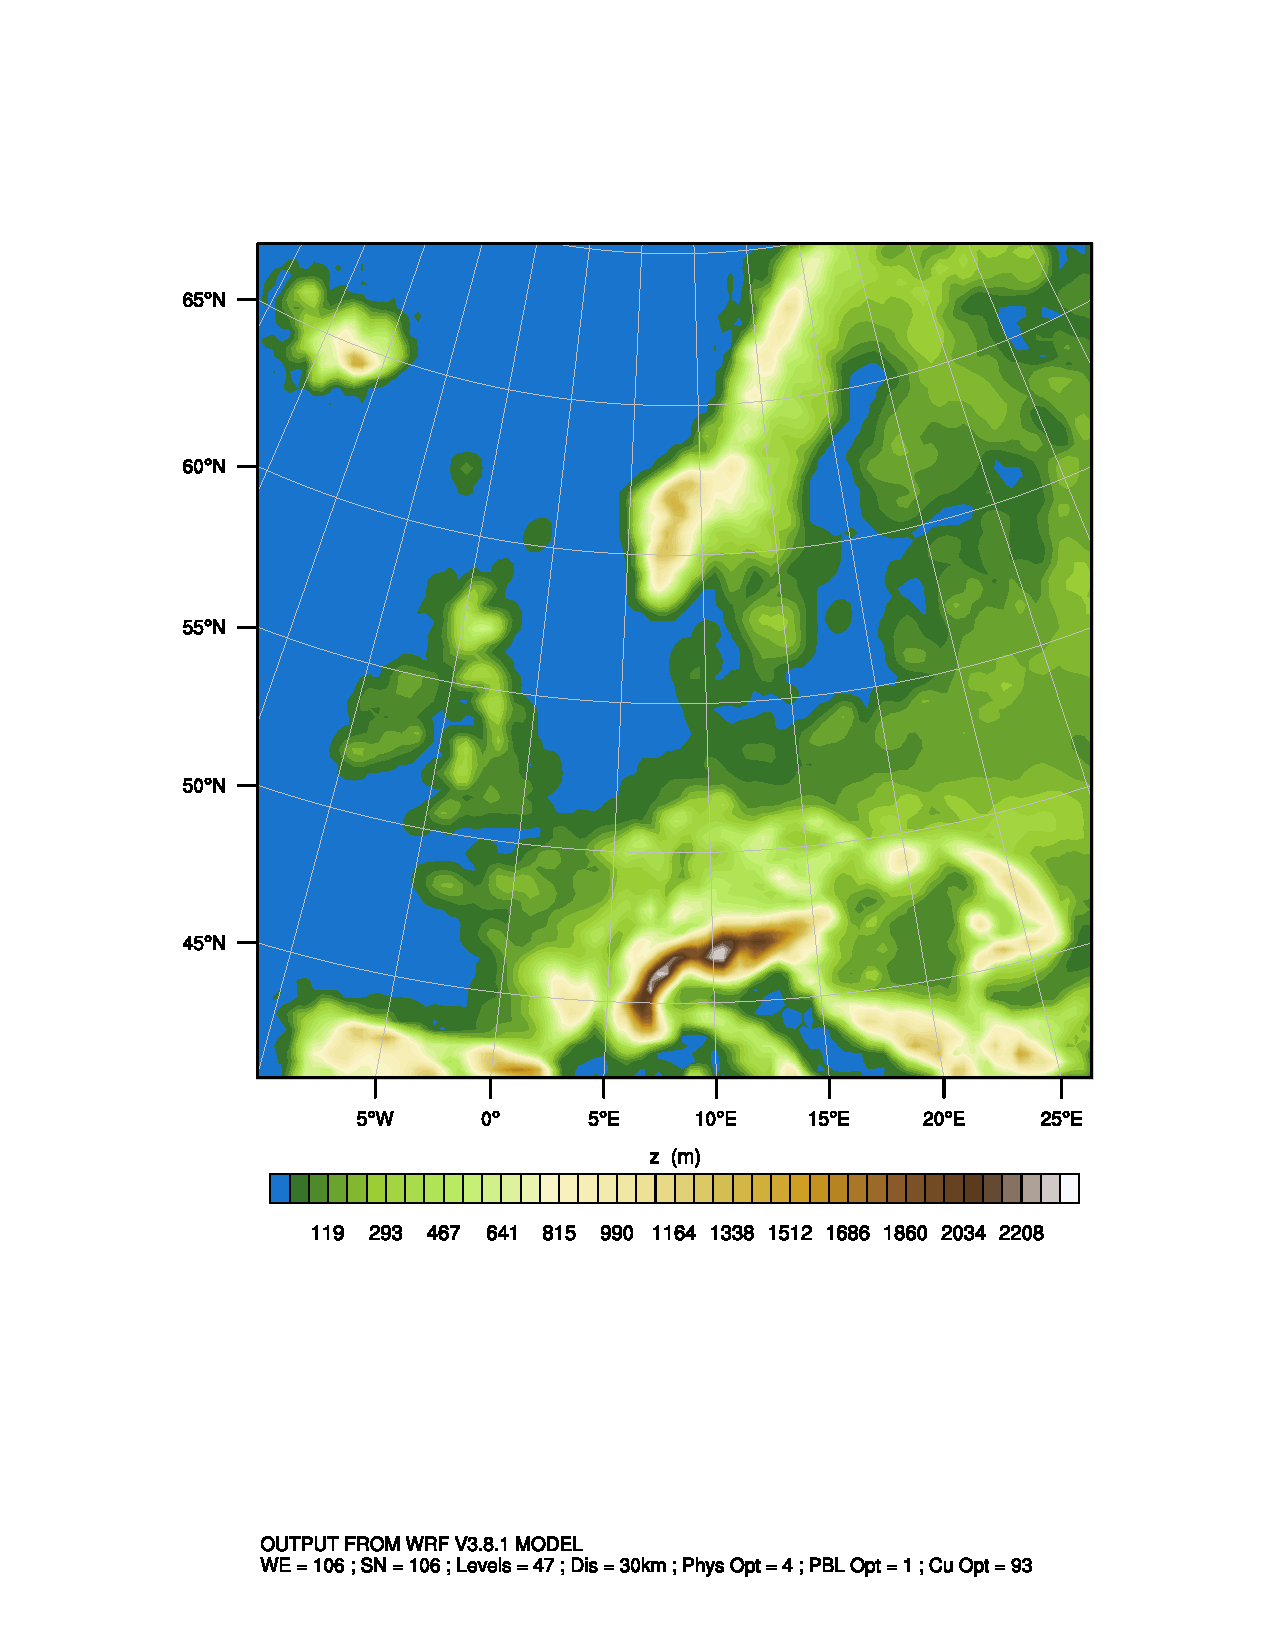
\includegraphics[width=0.25\linewidth,page=1,trim={2cm 6.5cm 1cm 3.5cm},clip]{Imagenes/05/hov_domain.pdf}%
	\includegraphics[width=0.25\linewidth,page=2,trim={2cm 6.5cm 1cm 3.5cm},clip]{Imagenes/05/hov_domain.pdf}%
	\includegraphics[width=0.25\linewidth,page=3,trim={2cm 6.5cm 1cm 3.5cm},clip]{Imagenes/05/hov_domain.pdf}%
	\includegraphics[width=0.25\linewidth,page=4,trim={2cm 6.5cm 1cm 3.5cm},clip]{Imagenes/05/hov_domain.pdf}%
	
	\bigskip
	\includegraphics[width=0.25\linewidth,page=5,trim={2cm 6.5cm 1cm 3.5cm},clip]{Imagenes/05/hov_domain.pdf}%
	\includegraphics[width=0.25\linewidth,page=6,trim={2cm 6.5cm 1cm 3.5cm},clip]{Imagenes/05/hov_domain.pdf}%
	\includegraphics[width=0.25\linewidth,page=7,trim={2cm 6.5cm 1cm 3.5cm},clip]{Imagenes/05/hov_domain.pdf}%
	\includegraphics[width=0.25\linewidth,page=8,trim={2cm 6.5cm 1cm 3.5cm},clip]{Imagenes/05/hov_domain.pdf}%
	
	\bigskip
	\includegraphics[width=0.25\linewidth,page=9,trim={2cm 6.5cm 1cm 3.5cm},clip]{Imagenes/05/hov_domain.pdf}%
	\includegraphics[width=0.25\linewidth,page=10,trim={2cm 6.5cm 1cm 3.5cm},clip]{Imagenes/05/hov_domain.pdf}%
	\includegraphics[width=0.25\linewidth,page=11,trim={2cm 6.5cm 1cm 3.5cm},clip]{Imagenes/05/hov_domain.pdf}%
	\includegraphics[width=0.25\linewidth,page=12,trim={2cm 6.5cm 1cm 3.5cm},clip]{Imagenes/05/hov_domain.pdf}%
	
	\bigskip
	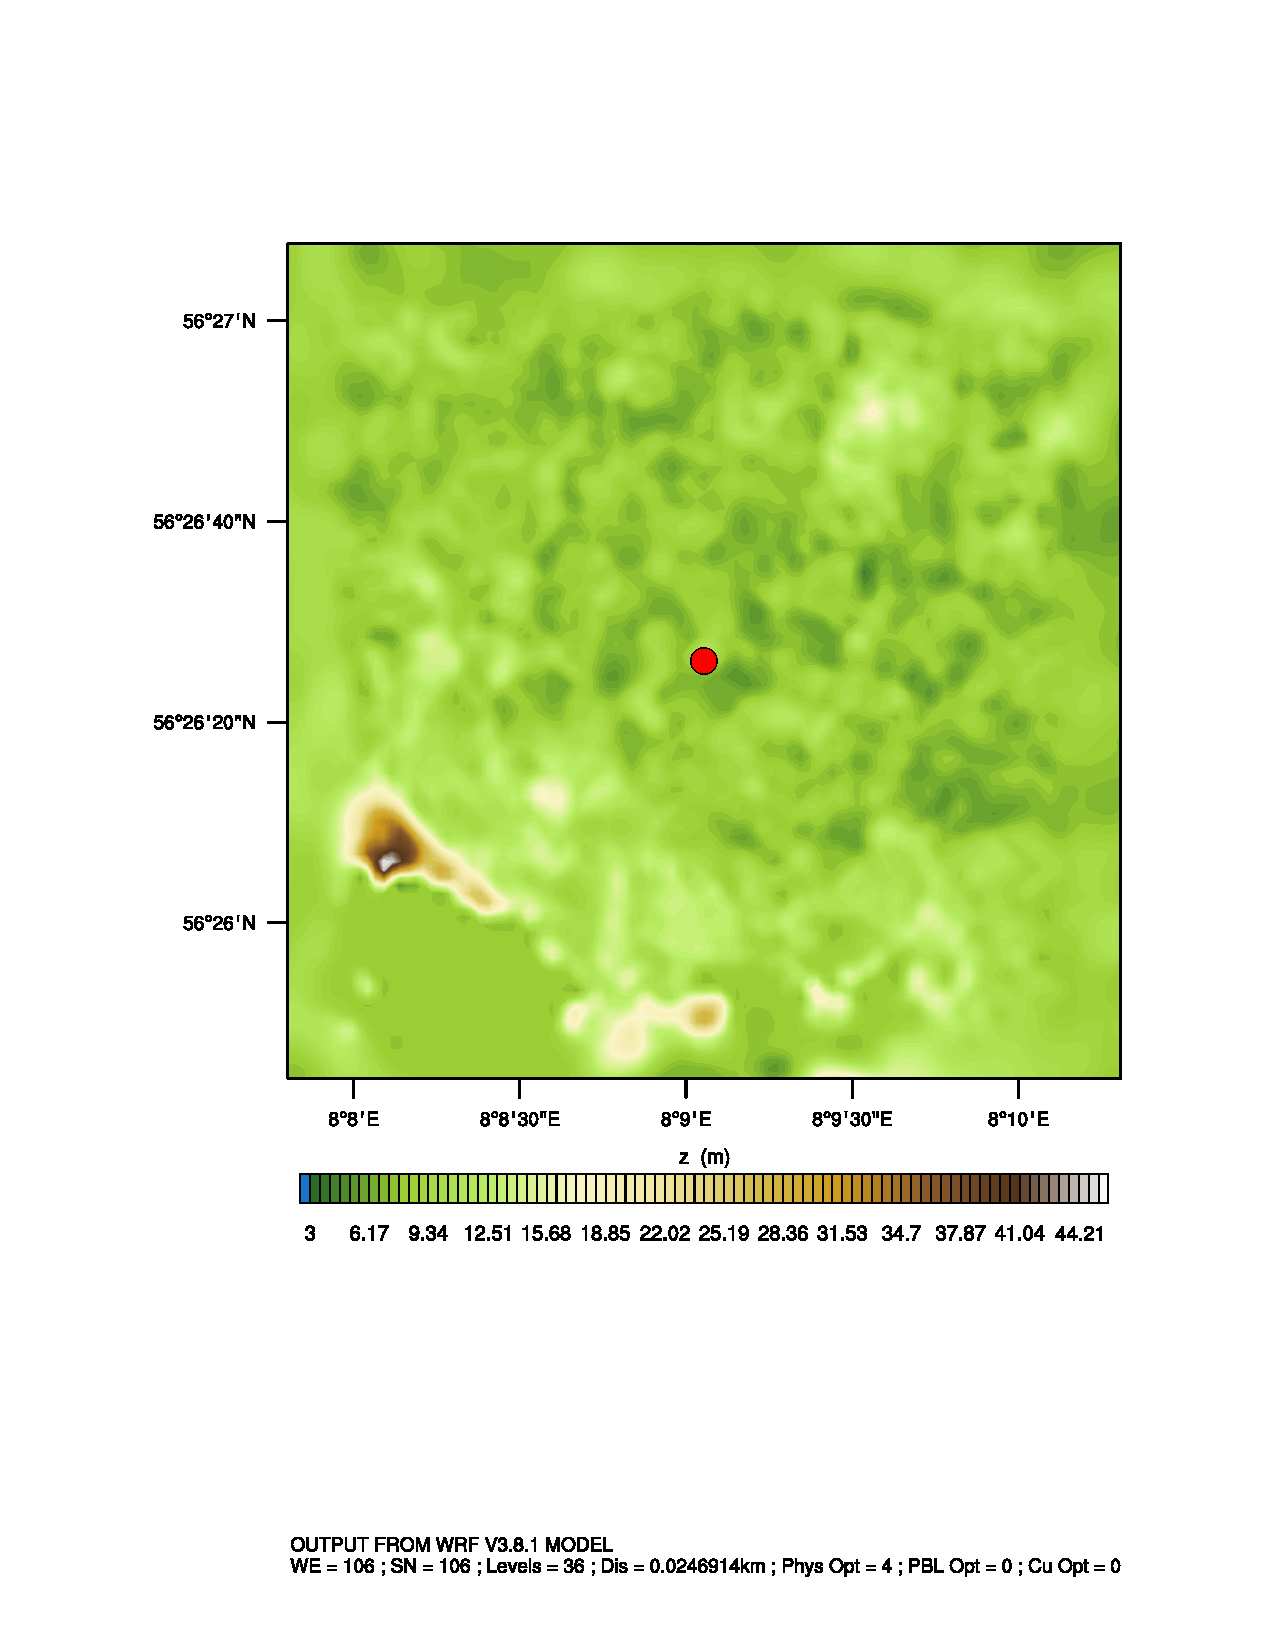
\includegraphics[width=0.25\linewidth,page=1,trim={2cm 6.5cm 1cm 3.5cm},clip]{Imagenes/05/hov_control_point.pdf}%
	\includegraphics[width=0.25\linewidth,page=14,trim={2cm 6.5cm 1cm 3.5cm},clip]{Imagenes/05/hov_domain.pdf}%
	
	\caption{Orografía (MSNM) y uso de suelo (categoría USGS24) de alta definición para cada uno de las mallas anidadas (d01-d07). Para el dominio d07 se presenta la ubicación del punto de control (rojo) y la distribución de turbinas eólicas en la zona (negro).}
	\label{fig:dominios}
\end{figure}
\newpage
\begin{figure}[H]
	\centering
	\begin{minipage}{0.5\linewidth}
		\center(a)
	\end{minipage}%
	\begin{minipage}{0.5\linewidth}
		\center(b)
	\end{minipage}%
	
	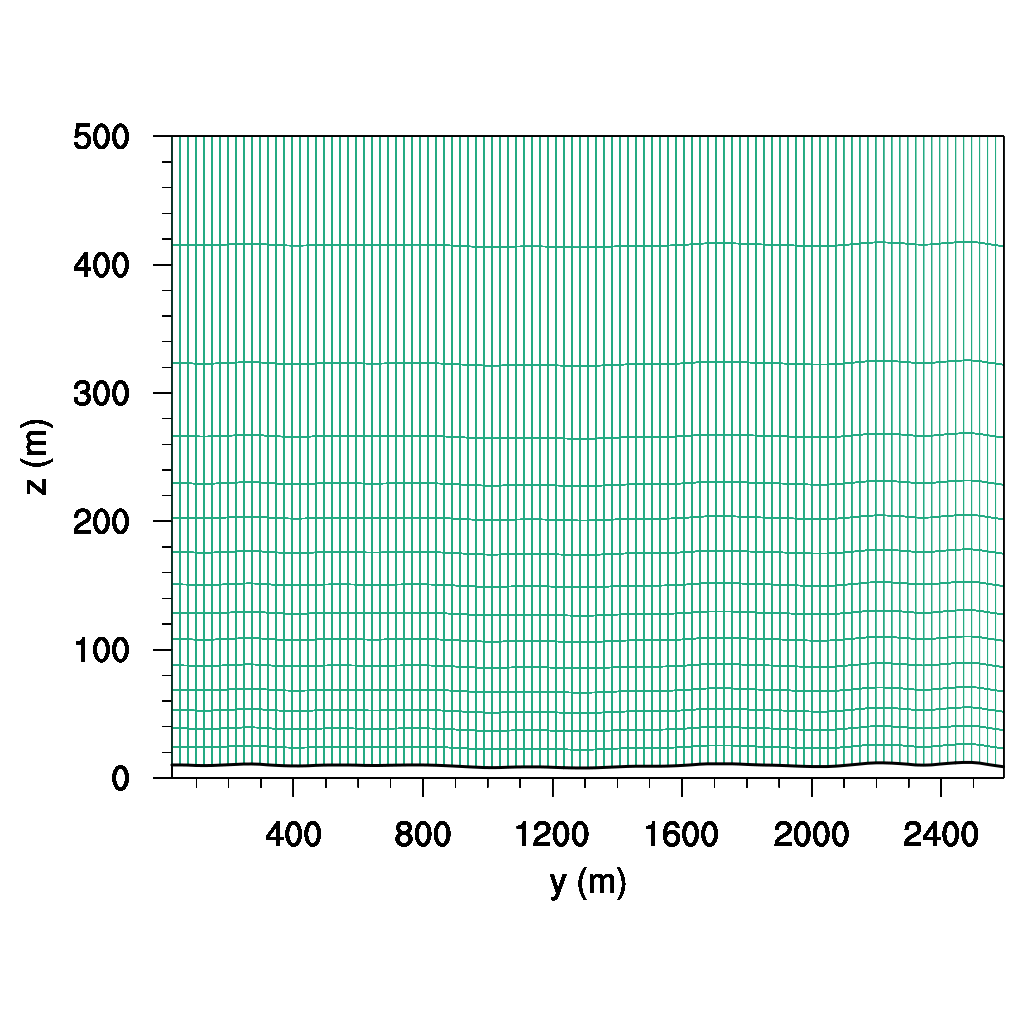
\includegraphics[width=0.5\linewidth,trim={0cm 4cm -2cm 4cm},clip]{Imagenes/05/hov_mesh_y000001}%
	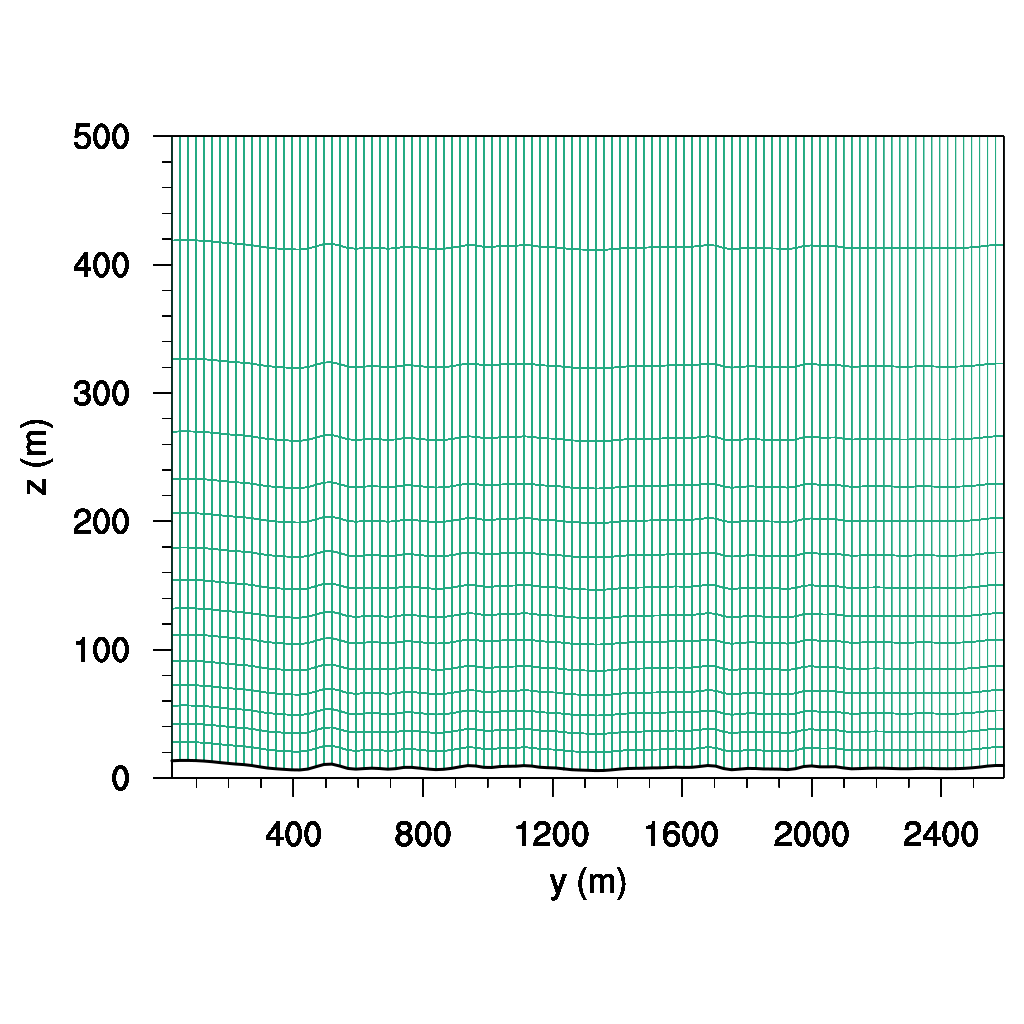
\includegraphics[width=0.5\linewidth,trim={0cm 4cm -2cm 4cm},clip]{Imagenes/05/hov_mesh_y000033}%
	
	\begin{minipage}{0.5\linewidth}
		\center(c)
	\end{minipage}%
	\begin{minipage}{0.5\linewidth}
		\center(d)
	\end{minipage}%
	
	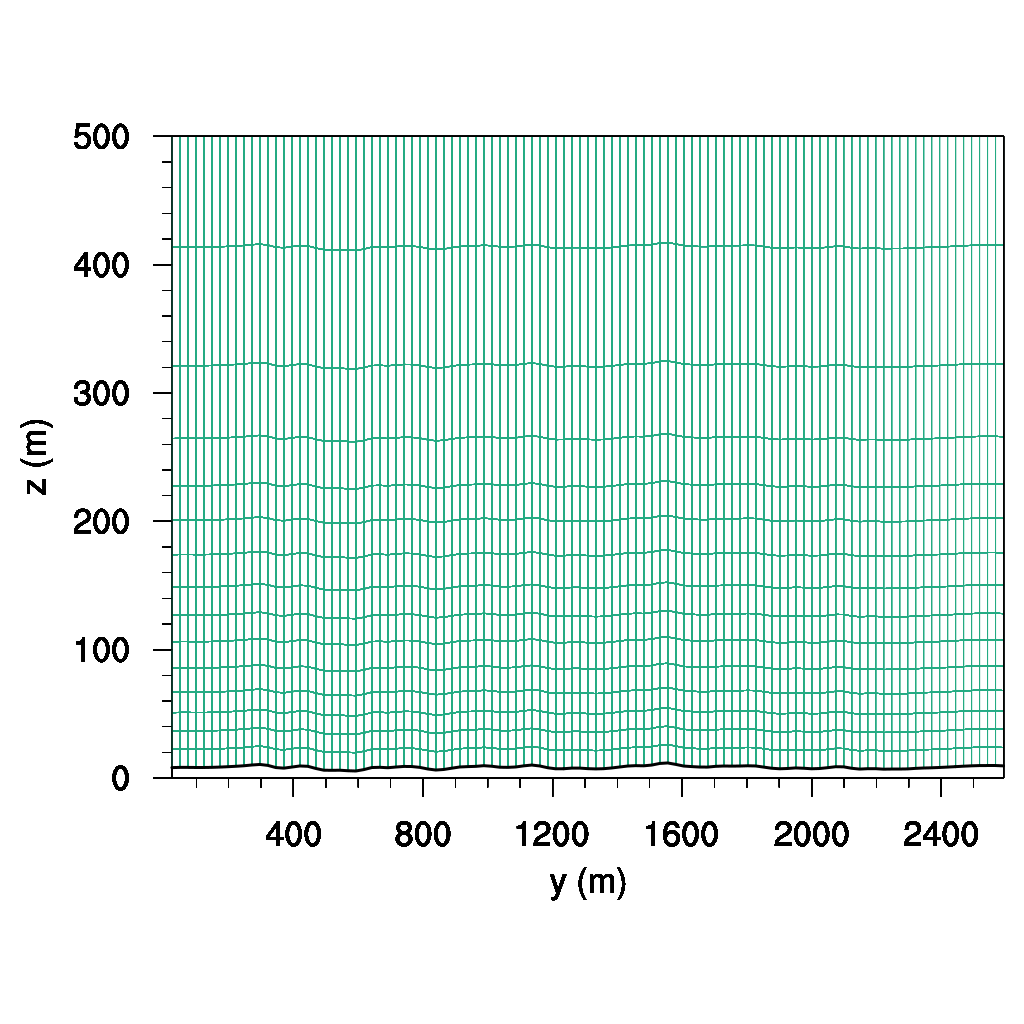
\includegraphics[width=0.5\linewidth,trim={0cm 4cm -2cm 4cm},clip]{Imagenes/05/hov_mesh_y000066}%
	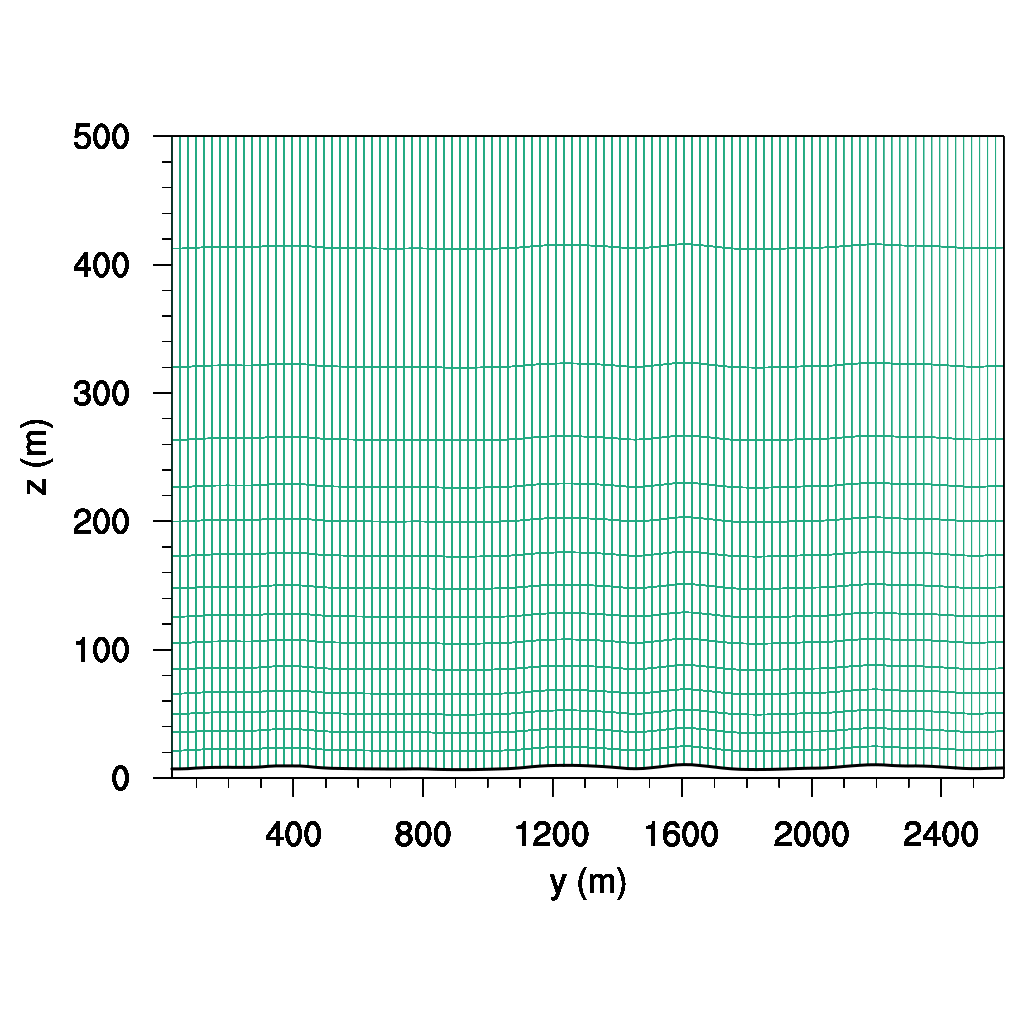
\includegraphics[width=0.5\linewidth,trim={0cm 4cm -2cm 4cm},clip]{Imagenes/05/hov_mesh_y000101}%
	
	\caption{Distribución de la malla vertical.}
	\label{fig:c1_mesh}
\end{figure}

\subsection{Aspectos generales del proceso de asimilación de datos}
A modo de implementar una mejora para la simulación multiescala a alta resolución que se está realizando, es que se plantea la utilización de un método de asimilación de datos para poder anclar ciertos valores conocidos dentro de la simulación y así obtener resultados mas acordes a la realidad.

La base teórica de la asimilación de datos en WRF ya se mencionó en informes anteriores. A continuación se presentan la información relevante para la correcta ejecución del sistema de asimilación y su replicabilidad.

\begin{table}[h!]
	\caption{Características del proceso de DA.}\label{tab:c2DA}
	\centering\footnotesize
	\begin{tabular}{lcc}
		\toprule
		Parámetro & Selección \\
		\midrule
		Hora Inicio	DA 	 & 06:00:00   \\
		Hora Término DA	 		 & 12:00:00  \\
		Intervalo de DA	&	10 mins. \\
		Puntos a Anidar	 	 & 5   \\
		Variables	& $u,v$   \\
		Lat. Mástil	& 56.440582   \\
		Lon. Mástil	& 8.150896   \\
		Alturas 	& 10m, 40m, 60m, 80m, 100m \\
		\bottomrule
	\end{tabular}
\end{table}

Los valores a asimilar son los valores tomados experimentalmente en el mástil meteorológico de Høvsøre y que se pueden ver en la Figura \ref{fig:ts_u}.

\newpage
\section{Caso de Estudio: Terreno Complejo Bolund}
\subsection{Aspectos generales de las simulaciones}
Tomando en cuenta que la campaña de medición para el caso Bolund se llevó a cabo durante los meses de Enero y Febrero del 2008, fue necesario hallar un día en donde hubiera una estratificación atmosférica lo mas neutra posible, con el modo de tener resultados comparables con aquellos obtenidos en la literatura y simulados de manera ideal.

Convenientemente, en el informe técnico que detalla la campaña de medición, los autores presentan un gráfico para la longitud de Monin-Obukhov que permite identificar que los días 3-4 de Enero presentan una estratificación muy cercana a la neutra y por lo tanto se decide simular para esas horas.
\begin{table}[h!]
	\caption{Dominio numerico espacial y temporal para simulación del caso Høvsøre.}\label{tab:c3exp}
	\centering\footnotesize
	\begin{tabular}{lcc}
		\toprule
		Parámetro & Selección \\
		\midrule
		Fecha	 	 & 04-01-2008   \\
		Hora Inicio	 	 & 06:00 UTM\\
		Hora Término	 		 & 20:00 UTM\\
		Puntos Malla Vert.	 	 & 50   \\
		$P_{top}$ 	& 10000 kPa\\
		\# Dominios	& 8   \\
		Lat. Centro	& 55.70360   \\
		Lon. Centro	& 12.09840   \\
		\bottomrule
	\end{tabular}
\end{table}

\begin{table}[H]
	\caption{Valores característicos de cada dominio.}\label{tab:c3val_carac}
	\centering\footnotesize
	\begin{tabular}{lllllllll}
		\toprule
		Dominio 				& d01	&	d02	&	d03	&	d04	&	d05	&	d06 &	d07&	d08 \\
		\midrule
		$N_x$		& 106 & 106 & 106 &106&106&106&106&106  \\
		$N_y$	 		& 106 & 106 & 106 &106&106&106&106&91  \\
		$\Delta x,\Delta y$	[m]	 		& 10000 & 3333.3 & 1111.1 &222.22&74.074&24.691&8.23045&2.74348  \\
		$\Delta t$	[s]	 		& 40 & 13.3333 & 4.4444 &0.8889&0.2963&0.0988&0.0329&0.0110  \\
		Orografía		 	& GMTED2010 & GMTED2010 & GMTED2010 &ASTER&ASTER&ASTER&ASTER&Bolund  \\
		Uso de Suelo					& USGS & USGS & USGS &CLC12&CLC12&CLC12&CLC12&Bolund \\
		\bottomrule
	\end{tabular}
\end{table}

\begin{table}[H]
	\caption{Parametrizaciones físicas utilizadas en el modelo.}\label{tab:c3param_fis}
	\centering\footnotesize
	\begin{tabular}{llllllll}
		\toprule
		Dominio 				& d01	&	d02	&	d03	&	d04	&	d05	&	d06 &	d07 \\
		\midrule
		Micro-físicas		 	& WSM5 & WSM5 & WSM5 &WSM5&WSM5&WSM5&WSM5  \\
		Cúmulos			 		& Grell & -- & -- & -- & -- & -- & -- \\ 
		Capa Superficial	 	& MM5 & MM5 & MM5 & MM5 & MM5 & MM5 & MM5 \\
		PBL				 		& YSU & YSU & YSU & -- & -- & -- & -- \\
		Modelo LES				 		& -- & -- & -- & 1.5TKE & 1.5TKE & 1.5TKE & 1.5TKE \\
		Modelo de Suelo 		& Difus. & Difus. & Difus. & Difus. & Difus. & Difus. & Difus. \\
		Rad. Onda Larga	& RRTM &RRTM&RRTM&RRTM&RRTM&RRTM&RRTM \\
		Rad. Onda Corta	& Dudhia &Dudhia&Dudhia&Dudhia&Dudhia&Dudhia&Dudhia \\
		\bottomrule
	\end{tabular}
\end{table}

\begin{figure}[H]
	\centering
	\includegraphics[width=0.48\linewidth,page=1,trim={5mm 3mm 3mm 3mm},clip,frame]{Imagenes/05/bol_d1-2-3-4edit.jpg}
	\includegraphics[width=0.48\linewidth,page=1,trim={5mm 3mm 3mm 3mm},clip,frame]{Imagenes/05/bol_d4-5-6edit.jpg}
	
	\bigskip
	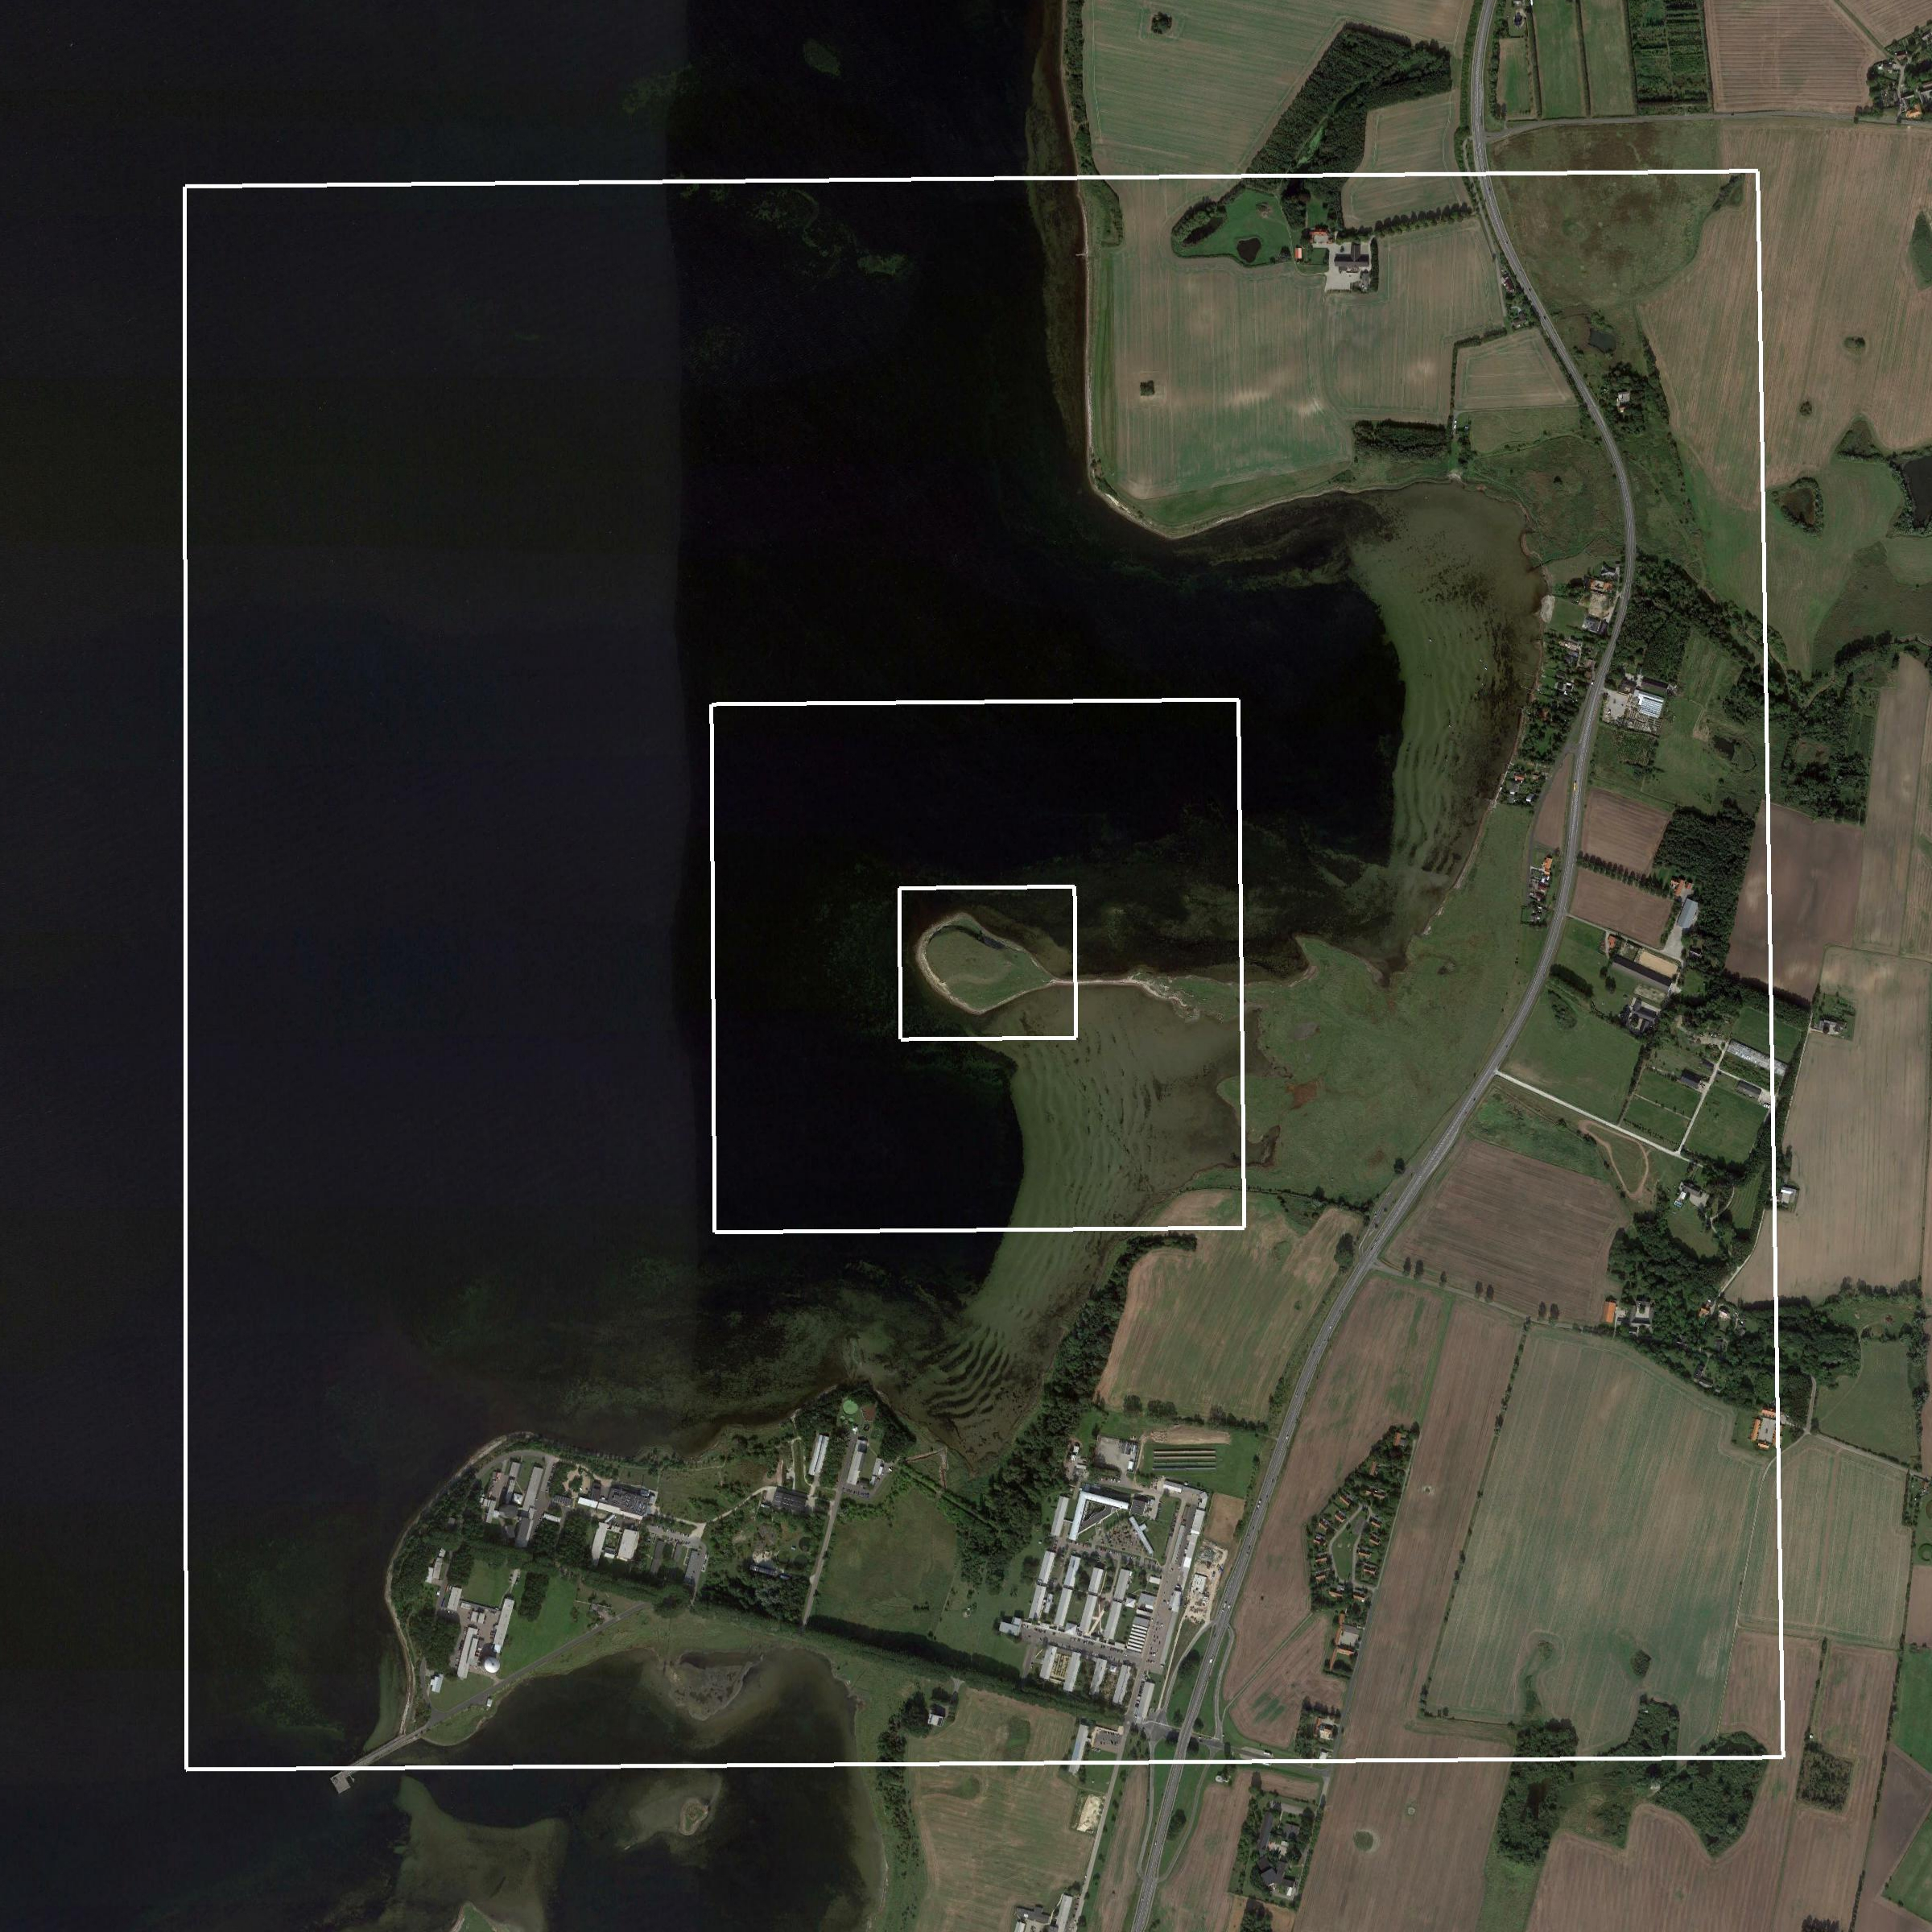
\includegraphics[width=0.6\linewidth,page=1,trim={5mm 3mm 3mm 3mm},clip,frame]{Imagenes/05/bol_d6-7-8edit.jpg}%
	
	\caption{Distribución telescópica de los 8 mallas anidadas en el dominio numérico.}
	\label{fig:c3dom_telesco}
\end{figure}

\begin{figure}[H]
	\centering
	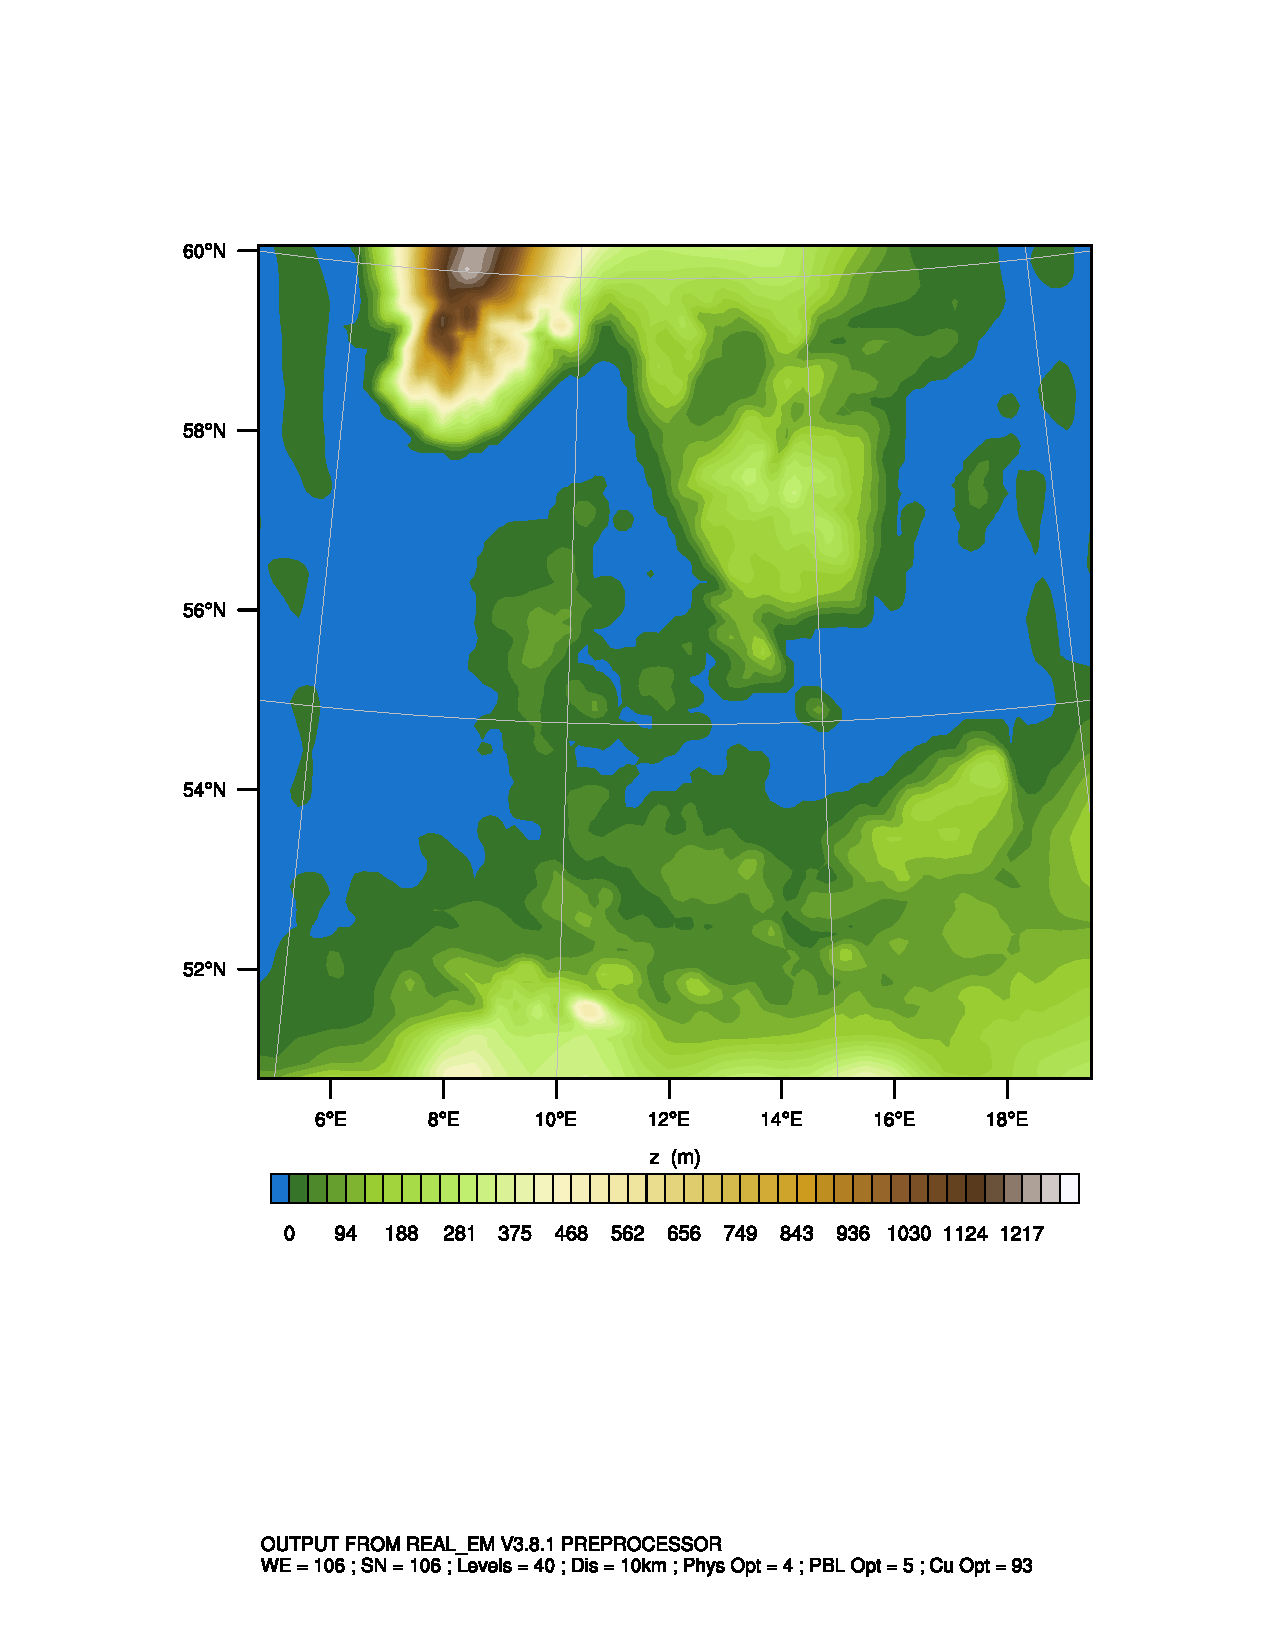
\includegraphics[width=0.25\linewidth,page=1,trim={2cm 6.5cm 1cm 3.5cm},clip]{Imagenes/05/bol_domain.pdf}%
	\includegraphics[width=0.25\linewidth,page=2,trim={2cm 6.5cm 1cm 3.5cm},clip]{Imagenes/05/bol_domain.pdf}%
	\includegraphics[width=0.25\linewidth,page=3,trim={2cm 6.5cm 1cm 3.5cm},clip]{Imagenes/05/bol_domain.pdf}%
	\includegraphics[width=0.25\linewidth,page=4,trim={2cm 6.5cm 1cm 3.5cm},clip]{Imagenes/05/bol_domain.pdf}%
	
	\bigskip
	\includegraphics[width=0.25\linewidth,page=5,trim={2cm 6.5cm 1cm 3.5cm},clip]{Imagenes/05/bol_domain.pdf}%
	\includegraphics[width=0.25\linewidth,page=6,trim={2cm 6.5cm 1cm 3.5cm},clip]{Imagenes/05/bol_domain.pdf}%
	\includegraphics[width=0.25\linewidth,page=7,trim={2cm 6.5cm 1cm 3.5cm},clip]{Imagenes/05/bol_domain.pdf}%
	\includegraphics[width=0.25\linewidth,page=8,trim={2cm 6.5cm 1cm 3.5cm},clip]{Imagenes/05/bol_domain.pdf}%
	
	\bigskip
	\includegraphics[width=0.25\linewidth,page=9,trim={2cm 6.5cm 1cm 3.5cm},clip]{Imagenes/05/bol_domain.pdf}%
	\includegraphics[width=0.25\linewidth,page=10,trim={2cm 6.5cm 1cm 3.5cm},clip]{Imagenes/05/bol_domain.pdf}%
	\includegraphics[width=0.25\linewidth,page=11,trim={2cm 6.5cm 1cm 3.5cm},clip]{Imagenes/05/bol_domain.pdf}%
	\includegraphics[width=0.25\linewidth,page=12,trim={2cm 6.5cm 1cm 3.5cm},clip]{Imagenes/05/bol_domain.pdf}%
	
	\bigskip
	\includegraphics[width=0.25\linewidth,page=13,trim={2cm 6.5cm 1cm 3.5cm},clip]{Imagenes/05/bol_domain.pdf}%
	\includegraphics[width=0.25\linewidth,page=14,trim={2cm 6.5cm 1cm 3.5cm},clip]{Imagenes/05/bol_domain.pdf}%
	
	\bigskip
	\includegraphics[width=0.25\linewidth,page=15,trim={0cm 6.5cm 1cm 3.5cm},clip]{Imagenes/05/bol_domain.pdf}%
	\includegraphics[width=0.25\linewidth,page=16,trim={0cm 6.5cm 1cm 3.5cm},clip]{Imagenes/05/bol_domain.pdf}%
	
	\caption{Orografía (MSNM) y uso de suelo (categoría USGS24) de alta definición para cada uno de las mallas anidadas (d01-d08).}
	\label{fig:c3dominios}
\end{figure}

\begin{figure}[H]
	\centering
	\includegraphics[width=0.9\linewidth,page=1,trim={0cm 6cm -1cm 4cm},clip]{Imagenes/05/bol_control_point.pdf}%
	\caption{Ubicación espacial de los puntos de control en el dominio. En cada punto de control se ubican anemómetros que miden a las alturas de 2m, 5m, y 9m.}
	\label{fig:c3control_points}
\end{figure}

\begin{figure}[H]
	\centering
	\begin{minipage}{0.5\linewidth}
		\center(a)
	\end{minipage}%
	\begin{minipage}{0.5\linewidth}
		\center(b)
	\end{minipage}%
	
	\includegraphics[width=0.5\linewidth,trim={3cm 0cm 0cm 0cm},clip]{Imagenes/05/bol_mesh_y000001}%
	\includegraphics[width=0.5\linewidth,trim={3cm 0cm 0cm 0cm},clip]{Imagenes/05/bol_mesh_y000022}%
	
	\begin{minipage}{0.5\linewidth}
		\center(c)
	\end{minipage}%
	\begin{minipage}{0.5\linewidth}
		\center(d)
	\end{minipage}%
	
	\includegraphics[width=0.5\linewidth,trim={3cm 0cm 0cm 0cm},clip]{Imagenes/05/bol_mesh_y000053}%
	\includegraphics[width=0.5\linewidth,trim={3cm 0cm 0cm 0cm},clip]{Imagenes/05/bol_mesh_y000090}%
	
	\caption{Distribución de la malla vertical.}
	\label{fig:c3_mesh}
\end{figure}

\subsection{Aspectos generales del proceso de asimilación de datos}

\begin{table}[h!]
	\caption{Características del proceso de DA.}\label{tab:c2DA}
	\centering\footnotesize
	\begin{tabular}{lcc}
		\toprule
		Parámetro & Selección \\
		\midrule
		Hora Inicio	DA 	 & 06:00:00   \\
		Hora Término DA	 		 & 12:00:00  \\
		Intervalo de DA	&	10 mins. \\
		Puntos a Anidar	 	 & ??   \\
		Variables	& $u,v$   \\
		Lat. Mástil	& ??   \\
		Lon. Mástil	& ??   \\
		Alturas 	& 2m, 5m, 9m \\
		\bottomrule
	\end{tabular}
\end{table}

%
\chapter{Resultados Obtenidos y Análisis}
A continuación se presentan los resultados de los 4 experimentos numéricos realizados. El orden de presentación será de la siguiente forma: (i) resultados para el caso Høvsore sin DA, es decir, la validación básica de la metodología, (ii) caso Høvsøre con DA puntual, (iii) caso Bolund sin DA y (iv) caso Bolund con DA multipunto. Todos los resultados son obtenidos de la malla interior refinada para cada dominio, es decir, d07 para Høvsore y d08 para Bolund. El cálculo de los espectros espaciales está hecho en base a: (a) valores obtenidos para un nivel $\eta$ en particular, (b) promedios temporales sobre las ventanas de tiempo válidas de simulación y sobre cada número de onda asociado a la discretización de la malla, y (c) un promedio móvil para eliminar ruido del espectro.
\section{Caso I: Høvsøre}
Tomando en consideración que los resultados para este caso son válidos desde las 12:00 hasta las 18:00 del día simulado, se busca evidenciar cuatro aspectos relevantes del modelo: (i) La respuesta del modelo LES al escalamiento dinámico y la alta resolución, (ii) la concordancia entre los datos simulados y aquellos obtenidos por \cite{Pea2013}, (ii) la concordancia entre los datos simulados y la serie de tiempo medida en el mástil meteorológico y (iv) la concordancia de los parámetros de segundo orden con aquellos canónicos para flujo en terreno plano homogéneo.

\subsubsection{Estratificación Térmica y Espesor de Capa Límite Atmosférica}
En primer lugar se revisa la estabilidad del flujo durante la ventana de tiempo seleccionada. Tomando en cuenta que según la literatura este debería ser un caso de atmósfera neutra, la Figura \ref{fig:06_hov_pbl} muestra la evolución del perfil de temperatura potencial virtual a través de toda la simulación para el punto de control en el mástil meteorológico. Debido a la homogeneidad del terreno, los perfiles de temperatura potencial virtual en el resto del dominio son, a grandes rasgos, idénticos, y por lo tanto se puede inferir que el perfil mostrado es representativo de todo el dominio. En éste se puede notar cómo la estratificación térmica del campo va cambiando a medida que avanza en el ciclo diurno la simulación, desde una atmósfera inestable en la mañana, hasta la alta estabilidad en la noche. Notar que, tal como lo expuso Peña, se tiene un perfil de estratificación térmica neutra desde las 12:00 hasta las 15:00 horas, ventana de tiempo que cae dentro de los resultados válidos del modelo y por ende, será en esta ventana en la cual se extraerán resultados.

\begin{figure}[H]
	\begin{minipage}{0.5\linewidth}
		\centering{\hspace{0.9cm}(a)}
	\end{minipage}%
	\begin{minipage}{0.5\linewidth}
		\centering{\hspace{0.6cm}(b)}
	\end{minipage}%
	
	\begin{minipage}{0.5\linewidth}
		\centering
		\includegraphics[width=0.86\linewidth,trim={0cm 5mm 0cm 0mm},clip]{Imagenes/06/hov/pbl}%
	\end{minipage}%
	\begin{minipage}{0.5\linewidth}
		\centering
		\includegraphics[width=0.86\linewidth,trim={0cm 5mm 0cm 0cm},clip]{Imagenes/06/hov/temp_profile}%
	\end{minipage}%
	
	\caption{Ciclo diurno-nocturno del perfil de temperatura potencial virtual en el mástil meteorológico en Høvsøre. (a) Resultados cada 20 minutos del perfil de $\theta_v$. (b) Detalle del perfil de $\theta_v$ dentro de la capa límite atmosférica ($\delta \approx 750$ [m]).}
	\label{fig:06_hov_pbl}
\end{figure}

En base a la misma Figura \ref{fig:06_hov_pbl} es posible estimar el \textbf{alto de la capa límite} como el punto en altura justo antes de la inversión térmica. Utilizando este acercamiento es fácil notar como el espesor de ABL varía durante el día desde un valor cercano a los 800 [m] hasta unos 400 [m] en la noche. Se decide utilizar un valor promedio de $\delta = 750$ [m] para adimensionalizar los resultados obtenidos.
\subsubsection{Estructuras del Campo de Velocidades}
Con respecto a las variables de primer orden y el rendimiento del LES, la Figura \ref{fig:06_hov_eta1} muestra los campos instantáneos de velocidad para el primer nivel vertical $z_1\approx 5.25$ [m] del dominio interior d07 a las 15:00\footnote{Si bien la selección de la hora es arbitraria, cualquier hora después de las 12:00 hubiese servido y de hecho el comportamiento del campo no varía mucho, debido a las condiciones termodinámicas.}.Se pueden apreciar las estructuras de flujo turbulento que revela el método LES sobre el campo de velocidades. 
\begin{figure}[H]
	\centering
	\begin{minipage}{0.5\linewidth}
		\center\hspace{0.3cm}(a)
	\end{minipage}%
	\begin{minipage}{0.5\linewidth}
		\center\hspace{0.3cm}(b)
	\end{minipage}%
	
	\includegraphics[width=0.5\linewidth,page=55,trim={2.5cm 6.2cm 1cm 4.5cm},clip]{Imagenes/06/hov/eta1_u}%
	\includegraphics[width=0.5\linewidth,page=55,trim={2.5cm 6.2cm 1cm 4.5cm},clip]{Imagenes/06/hov/eta1_v}%
	
	\center{\hspace{0.3cm}(c)}
	
	\includegraphics[width=0.5\linewidth,page=55,trim={2.5cm 6.2cm 1cm 4.5cm},clip]{Imagenes/06/hov/eta1_V}%
	\caption{(a) Componente longitudinal $u$ de la velocidad en el primer nivel de la coordenada vertical ($z_1=5.25$ [m]) para las 15:00. (b) Idéntico al anterior pero para la componente transversal $v$. (c) Magnitud del campo de velocidad.}
	\label{fig:06_hov_eta1}
\end{figure}
A primera vista, se puede concluir que el método LES fue aplicado correctamente en el dominio, presentando las estructuras clásicas que se deberían manifestar en el campo de velocidades. En particular, para este caso se puede ver que las estructuras de flujo tienen cierto estiramiento desviándose del comportamiento clásico homogéneo. Esto se explica debido a la dirección preferente que tiene el viento proveniente del este (viento a $105^\circ$). La baja de velocidad local que se genera en la esquina inferior derecha se explica debido a la depresión topográfica local que existe en esa zona.
\subsubsection{Comparación de Series de Tiempo}
Para evaluar la calidad del modelo, se muestra la serie de tiempo de los datos simulados junto a lo datos medidos en el mástil meteorológico para la fecha de interés en la Figura \ref{fig:06_hov_ts}. 

\begin{figure}[H]
	\centering
	\includegraphics[width=1\linewidth,trim={9mm 63mm 10mm 55mm},clip]{Imagenes/06/hov/ts_v}%
	
	\includegraphics[width=1\linewidth,trim={12mm 55mm 10mm 55mm},clip]{Imagenes/06/hov/ts_o}%
	\caption{Serie de tiempo para la rapidez instantánea del viento $V$ y su dirección en la ubicación del mástil meteorológico. La línea continua corresponde a lo datos simulados interpolados a las alturas de medición (solo para $V$) y la línea punteada a los datos medidos en el mástil.}
	\label{fig:06_hov_ts}
\end{figure}

En la Figura \ref{fig:06_hov_ts}, la línea segmentada vertical indica el límite del tiempo de \emph{spinup} y por lo tanto sólo los resultados desde ese punto en adelante son válidos. Se puede apreciar que la simulación (en línea continua) capta de buena forma la tendencia de la magnitud de la velocidad para el mástil, sin embargo, la simulación fue incapaz de representar la aceleración del fluido en esa fecha. Un déficit de momentum se observa en los niveles superficiales, dando a entender que quizás el modelo de superficie o de turbulencia está actuando de manera disipativa en esos primeros niveles. Con respecto a la dirección del viento, ésta quedó a grandes rasgos bien representada por la simulación.

\begin{figure}[H]
	\begin{minipage}{0.33\linewidth}
		\centering \hspace{1.5cm}(a)
	\end{minipage}%
	\begin{minipage}{0.33\linewidth}
		\centering \hspace{1cm}(b)
	\end{minipage}%
	\begin{minipage}{0.33\linewidth}
		\centering \hspace{1cm}(c)
	\end{minipage}%
	\vspace{-3mm}
	\begin{center}
	\includegraphics[height=0.62\linewidth,page=37,trim={35mm 10mm 41mm 25mm},clip]{Imagenes/06/hov/9u}%
	\includegraphics[height=0.62\linewidth,page=37,trim={48mm 10mm 41mm 25mm},clip]{Imagenes/06/hov/9v}%
	\includegraphics[height=0.62\linewidth,page=37,trim={48mm 10mm 41mm 25mm},clip]{Imagenes/06/hov/9V}%
	\end{center}
	\caption{Comparación de la simulación con WRF (línea continua) con la simulación de \cite{Pea2013} (línea punteada) y valores medidos para (a) componente longitudinal $u$ de la velocidad del viento, (b) componente transversal $v$ y (c) magnitud de la velocidad del viento. Los datos corresponden a promedios temporales entre las 12:00 y 15:00, y han sido rotados de tal forma que su dirección sea 0$^\circ$ a los 10m sobre el suelo, igualando lo representado por \cite{Pea2013}.}
	\label{fig:06_hov_peña}
\end{figure}

\subsubsection{Validación con Peña et al. (2013)}
En la Figura \ref{fig:06_hov_peña} se muestran los resultados promediados para el intervalo definido neutro en este caso, junto con las mediciones experimentales y la simulación mesoescala de \cite{Pea2013}. Basándonos en estos resultados, se puede deducir que la simulación se comporta según lo esperado, encontrándose dentro de los márgenes de error de las mediciones. Además, la simulación meso-microescala con LES logra representar de mejor manera la rotación de la componente transversal $v$ que la simulación mesoescala hecha por \cite{Pea2013} Al igual que en los resultados de la serie de tiempo, existen grandes déficit de momentum cerca de la superficie por el modelo WRF. Sin embargo, el éxito de esta comparación da por validado el modelo LES multiescala planteado, dando espacio a que la asimilación de datos pueda corregir los déficit planteados.
\subsubsection{Variables de Segundo Orden}
Los resultados mostrados en la Figura \ref{fig:06_hov_mean_secondorder} servirán como benchmark para posteriores análisis que expondrán las variables de segundo orden relevantes para flujos atmosféricos dentro de la ABL. 

Con respecto a la energía cinética de submalla $k_{sgs}$ y al esfuerzo de Reynolds $\tau_{13}$, se puede ver que estos se comportan según lo esperado en un flujo cercano a la pared. Sus valores están dentro de los valores característicos presentados en la literatura, presentando ciertas desviaciones debido al carácter real de las simulaciones hechas por WRF. Estos resultados permiten confirmar que el modelo de turbulencia, el modelo de pared (suelo), y el de capa superficial se comportan de manera adecuada para una simulación a alta resolución.

La adimensionalización de las variables se llevó a cabo con la velocidad de fricción $u_*$ promedio, calculado entre las horas en donde el dominio se mantuvo con estratificación térmica neutra y obtenido para el punto de control donde se ubica el mástil. El valor de $u_*$ es un resultados de la física parametrizada por el modelo de suelo.

\begin{figure}[H]
	\begin{minipage}{0.33\linewidth}
		\centering \hspace{1cm}(a)
	\end{minipage}%
	\begin{minipage}{0.33\linewidth}
		\centering \hspace{0.8cm}(b)
	\end{minipage}%
	\begin{minipage}{0.33\linewidth}
		\centering \hspace{0.5cm}(c)
	\end{minipage}%
	\vspace{-4mm}
	\begin{center}
	\includegraphics[height=0.5\linewidth,page=1,trim={6mm 5mm 3mm 0mm},clip]{Imagenes/06/hov/mean_data}%
	\includegraphics[height=0.5\linewidth,page=2,trim={12mm 5mm 3mm 0mm},clip]{Imagenes/06/hov/mean_data}%
	\includegraphics[height=0.5\linewidth,page=3,trim={12mm 5mm 3mm 0mm},clip]{Imagenes/06/hov/mean_data}%
	\end{center}
	\caption{Variables adimensionalizadas (con $u_* = 0.552$ [m/s]) de segundo orden para el caso de Høvsøre promediados entre las 12:00 y las 15:00 (atmósfera neutra, terreno plano homogéneo). (a) Energía cinética turbulenta de submalla, (b) Gradiente de velocidad, (c) Esfuerzo turbulento. }
	\label{fig:06_hov_mean_secondorder}
\end{figure}

Con respecto al gradiente adimensional $\Phi_m$, el valor que maneja la teoría de Monin-Obukhov para atmósfera neutra es unitario. En este caso se tiene un valor sobrestimado cercano a $3$ con un ligero \emph{overshoot} en el primer 20\% de la capa límite. El overshoot puede ser entendido según \cite{doi:10.1063/1.3319073} como un LES que no cumple los criterios adecuados para escalar correctamente el flujo superficial de pared. El modelo WRF, siendo un modelo climático, utiliza su parametrización de capa superficial para hacerse cargo de este problema, sin embargo en este caso se muestra deficiente. Con respecto a la diferencia de valores, se puede ver como la influencia del terreno real no homogéneo y el uso de las condiciones de borde provenientes de otro modelo real desplaza la curva hacia la derecha.

Finalmente, la Figura \ref{fig:06_hov_spectrum} muestra el espectro espacial bidimensional para los primeros 5 niveles verticales del modelo. Se aprecia la desviación de la pendiente inercial para el primer nivel debido a la influencia del terreno en comparación a los niveles superiores que presentan una mayor concordancia con la ley de los -5/3. El filtro corta efectivamente a nivel de malla en el número de onda correspondiente a $(2\Delta x)^{-1}\approx 0.02$ [1/m] y por lo tanto está siendo bien aplicado. La forma del espectro, exhibiendo el ingreso de energía en las escalas mas grandes y la disipación después del número de onda de corte, muestra concordancia con la fenomenología física de los flujos turbulentos y por lo tanto se puede argumentar que el modelo WRF representa correctamente la cascada de energía en su modo LES a alta resolución sobre terreno plano.
\begin{figure}[H]
	\centering
	\includegraphics[width=1.0\linewidth,page=1,trim={3mm 5mm 3mm 3mm},clip]{Imagenes/06/hov/spectra}%
	\caption{Espectros de energía cinética para la magnitud horizontal del viento a distintos niveles verticales en el dominio d07 caso Høvsøre.}
	\label{fig:06_hov_spectrum}
\end{figure}

\subsubsection{Parámetros Estadísticos y Dispersión}
La Figura \ref{fig:06_corr_hov} muestra el gráfico de dispersión entre la rapidez simulada y la medida en el mástil a las 6 alturas de interés. Para cada altura se muestra en la figura su coeficiente de correlación de Pearson respectivo. Considerando que el gráfico ideal debiese ser una recta diagonal, se puede ver que el modelo numérico WRF tuvo problemas con representar las altas velocidades a nivel de superficie. La consecuencia de esto, es que los valores para el coeficiente de correlación son bajos.
\begin{figure}[H]
	\centering
	\includegraphics[width=0.55\linewidth,page=1,trim={0cm 0cm 0cm 0cm},clip]{Imagenes/06/hov/corr}%
	\caption{Gráfico de dispersión para las velocidades a distintas alturas en el mástil meteorológico de Høvsøre. Cada color corresponde a los valores cada 10 minutos desde las 12:00 horas.}
	\label{fig:06_corr_hov}
\end{figure}

Con respecto al resto de los parámetros de error estadísticos, se tiene un valor para el MAE de $2.41091$ [m/s] y un valor para el RMSE de $2.80142$ [m/s]. Es decir, en promedio existe un error de aproximadamente 2 [m/s] para la rapidez del viento en los niveles analizados. Este error evidentemente es no deseable para evaluación del recurso eólico y se buscará corregir con la asimilación de datos 4D que se muestran más adelante.













\newpage
\section{Caso I: Høvsøre con Asimilación Puntual de Datos}
\subsubsection{Comparación Series de Tiempo}
Se revisa ahora la influencia que tiene la asimilación de datos en un solo punto para el caso del terreno real plano. En la Figura \ref{fig:06_hov_da_ts} se muestra la serie de tiempo de los datos para este caso. Se puede notar como en las primeras 6 horas se simulación se hace tender al campo a sus valores medidos, indicando la correcta aplicación del DA. 
\begin{figure}[H]
	\centering
	\includegraphics[width=1\linewidth,trim={9mm 63mm 10mm 55mm},clip]{Imagenes/06/hov_da/ts_v}%
	
	\includegraphics[width=1\linewidth,trim={12mm 55mm 10mm 55mm},clip]{Imagenes/06/hov_da/ts_o}%
	\caption{Serie de tiempo para la rapidez instantánea del viento $V$ y su dirección en la ubicación del mástil meteorológico para el caso con asimilación puntual de datos. La línea continua corresponde a lo datos simulados interpolados a las alturas de medición (solo para $V$) y la línea punteada a los datos medidos en el mástil.}
	\label{fig:06_hov_da_ts}
\end{figure}
Con respecto a los resultados simulados y válidos (luego del \emph{spinup}), estos nuevamente no logran captar la aceleración, ni tampoco suplir las deficiencias de viento a nivel de superficie. Una explicación para esto se puede encontrar en el mismo gráfico: la información asimilada pierde su influencia unos pocos pasos de tiempo después de ser asimilada. De esta forma la corrección que genera la asimilación de datos en la capa límite es poco efectiva, ya que el forzamiento de las condiciones de borde provenientes de la malla del dominio padre (d06) es superior al forzamiento generado por la asimilación.

De todas formas se obtiene una mejora, dado que la asimilación de datos logra influir en el comportamiento del flujo, acercando los valores de la velocidad a aquellos medidos por el mástil.

\begin{figure}[H]
	\begin{minipage}{0.33\linewidth}
		\centering \hspace{1cm}(a)
	\end{minipage}%
	\begin{minipage}{0.33\linewidth}
		\centering \hspace{0.8cm}(b)
	\end{minipage}%
	\begin{minipage}{0.33\linewidth}
		\centering \hspace{1cm}(c)
	\end{minipage}%
	\vspace{-7mm}
	\begin{center}
	\includegraphics[height=0.61\linewidth,page=37,trim={35mm 10mm 38mm 25mm},clip]{Imagenes/06/hov_da/9u}%
	\includegraphics[height=0.61\linewidth,page=37,trim={48mm 10mm 38mm 25mm},clip]{Imagenes/06/hov_da/9v}%
	\includegraphics[height=0.61\linewidth,page=37,trim={48mm 10mm 38mm 25mm},clip]{Imagenes/06/hov_da/9V}%
	\end{center}
	\caption{Comparación de la simulación con WRF+DA (línea continua) con la simulación de \cite{Pea2013} (linea punteada) y valores medidos para (a) componente longitudinal $u$ de la velocidad del viento, (b) componente transversal $v$ y (c) magnitud de la velocidad del viento. Los datos corresponden a promedios temporales entre las 12:00 y 15:00, y han sido rotados de tal forma que su dirección sea 0$^\circ$ a los 10m sobre el suelo.}
	\label{fig:06_hov_da_peña}
\end{figure}
\subsubsection{Comparación con Peña et al. (2013)}
Con respecto a los valores declarados por \cite{Pea2013}, la comparación se muestra en la Figura \ref{fig:06_hov_da_peña}. Estos siguen siendo válidos, estando dentro de las barras de error y se comportan cercano a lo medido. Los valores de superficie mejoran con respecto a su contraparte sin asimilación, pero el giro de la componente $v$ se pierde levemente debido a la corrección. Cabe mencionar que los resultados para esta simulación de la estratificación térmica se mantuvieron constantes, por lo que se continúa utilizando una altura de ABL de $\delta=750$ [m].
\subsubsection{Variables de Segundo Orden}
Para las variables de segundo orden, los comportamiento de $k_{sgs}$ y $\tau_{13}$ mantienen su forma esperada para el caso con DA. El gradiente adimensional de velocidad $\Phi_M$ se corrige levemente acercándose al valor canónico unitario cerca de la superficie, pero el \emph{overshoot} se incrementa superando ampliamente el valor de $4$ fuera de la capa superficial.

\begin{figure}[H]
	\begin{minipage}{0.33\linewidth}
		\centering \hspace{1cm}(a)
	\end{minipage}%
	\begin{minipage}{0.33\linewidth}
		\centering \hspace{0.8cm}(b)
	\end{minipage}%
	\begin{minipage}{0.33\linewidth}
		\centering \hspace{0.5cm}(c)
	\end{minipage}%
	\vspace{-4mm}
	\begin{center}
		\includegraphics[height=0.5\linewidth,page=1,trim={6mm 5mm 3mm 0mm},clip]{Imagenes/06/hov_da/mean_data}%
		\includegraphics[height=0.5\linewidth,page=2,trim={12mm 5mm 3mm 0mm},clip]{Imagenes/06/hov_da/mean_data}%
		\includegraphics[height=0.5\linewidth,page=3,trim={12mm 5mm 3mm 0mm},clip]{Imagenes/06/hov_da/mean_data}%
	\end{center}
	\caption{Variables adimensionalizadas (con $u_* = 0.527$ [m/s]) de segundo orden para el caso de Høvsøre con DA promediados entre las 12:00 y las 15:00 (atmósfera neutra, terreno plano homogéneo). (a) Energía cinética turbulenta de submalla, (b) Gradiente de velocidad, (c) Esfuerzo turbulento. }
	\label{fig:06_hov_da_mean_secondorder}
\end{figure}

El espectro de energía cinética horizontal en la Figura \ref{fig:06_hov_da_spectrum} nos muestra el impacto de la asimilación de datos a nivel de microescala. Si bien, en los niveles superiores no existe mayor diferencia con respecto al experimento sin asimilación, el nivel superficial exhibe una retro-distribución (\emph{backscatter}) de energía de submalla. Este ingreso de energía evidentemente proviene de la incorporación sintética por asimilación variacional de los valores medidos al modelo, los cuales se acentúan en el primer nivel. Surge la necesidad ahora de controlar este ingreso sintético de energía, a modo de tener resultados físicos para el problema. Esta necesidad se podría suplir a nivel de la clausura del LES para la modelación de la turbulencia.

\begin{figure}[H]
	\centering
	\includegraphics[width=1.0\linewidth,page=1,trim={3mm 5mm 3mm 3mm},clip]{Imagenes/06/hov_da/spectra}%
	\caption{Espectros de energía cinética para la magnitud horizontal del viento a distintos niveles verticales en el dominio d07 caso Høvsøre con DA.}
	\label{fig:06_hov_da_spectrum}
\end{figure}

\subsubsection{Parámetros Estadísticos y Dispersión}
Con respecto a las métricas estadísticas de error del experimento, el gráfico de dispersión asociado se puede ver en la Figura \ref{fig:06_corr_hov_da}. Acá se puede ver claramente que, en comparación al experimento anterior, existe una mejora acercando los resultados simulados a los datos medidos en terreno. Todos los coeficientes de correlación mejoraron, tal como se podría esperar para este caso, sin embargo aún se encuentran lejanos de un valor unitario o línea diagonal.
\begin{figure}[H]
	\centering
	\includegraphics[width=0.55\linewidth,page=1,trim={0cm 0cm 0cm 0cm},clip]{Imagenes/06/hov_da/corr}%
	\caption{Gráfico de dispersión para las velocidades a distintas alturas en el mástil meteorológico de Høvsøre (con DA). Cada color corresponde a los valores cada 10 minutos desde las 12:00 horas.}
	\label{fig:06_corr_hov_da}
\end{figure}

Finalmente, un resumen de las métricas de error se presentan en la Tabla \ref{tab:06_hov_mae_rmse}, indicando el porcentaje de mejora que se obtuvo gracias a la implementación de la asimilación de datos en un punto de control.

\begin{table}[H]
	\caption{Comparación de métricas para el caso I Høvsøre.}
	\label{tab:06_hov_mae_rmse}
	\centering%\footnotesize
	\begin{tabular}{lcc}
		\toprule
		& Sin DA & Con DA \\
		\midrule
		MAE & 2.41091 m/s & 2.16742 m/s \\
		RMSE & 2.80142 m/s& 2.55778 m/s\\
		$\Delta{RMSE}$& --  & $8.70\%$  \\
		$\Delta{MAE}$ & -- & $10.47\%$  \\
		\bottomrule
	\end{tabular}
\end{table}

















\newpage
\section{Caso II: Bolund}
Tomando como antecedente la mejora lograda por la metodología del LES a alta definición con DA en terreno plano, ahora se revisan los resultados obtenidos para la simulación de viento en terreno complejo utilizando una asimilación multipunto a nivel de superficie. Se buscará evidenciar en estos resultados: (i) el comportamiento del modelo WRF en su modo LES a muy alta resolución con y sin DA, (ii) el rendimiento de la simulación para obtener resultados comparables con aquellos representados en la comparación ciega de \cite{Bechmann2011}, (iii) la capacidad de representar fehacientemente las series de tiempo para la rapidez del viento en los 8 mástiles del dominio d08 en función de los parámetros estadísticos asociados y (iv) la forma que adquieren las variables relevantes de segundo orden para un caso real en terreno complejo.

\vspace*{\fill}
\begin{figure}[H]
	\begin{minipage}{0.5\linewidth}
		\centering{\hspace{0.9cm}(a)}
	\end{minipage}%
	\begin{minipage}{0.5\linewidth}
		\centering{\hspace{0.6cm}(b)}
	\end{minipage}%
	
	\begin{minipage}{0.5\linewidth}
		\centering
		\includegraphics[width=0.9\linewidth,trim={0cm 5mm 0cm 0mm},clip]{Imagenes/06/bol/mean_pbl}%
	\end{minipage}%
	\begin{minipage}{0.5\linewidth}
		\centering
		\includegraphics[width=0.9\linewidth,trim={0cm 5mm 0cm 0cm},clip]{Imagenes/06/bol/mean_profile}%
	\end{minipage}%
	
	\caption{Ciclo horario del perfil de temperatura potencial virtual promedio de los 8 mástiles en Bolund. (a) Resultados cada 10 minutos del perfil de $\theta_v$. (b) Detalle del perfil de $\theta_v$ dentro de la capa límite atmosférica con resultados cada 15 minutos ($\delta\approx300$ [m]).}
	\label{fig:06_bol_pbl}
\end{figure}
\vspace*{\fill}
\newpage
\subsubsection{Estratificación Térmica y Espesor de Capa Límite Atmosférica}
De manera análoga al Caso I, primero se revisará el estado de la estratificación térmica, y se contrastará con aquella declarada para la campaña experimental de Bolund (atmósfera neutra). 

La Figura \ref{fig:06_bol_pbl} muestra la evolución del perfil de temperatura potencial virtual promedio de los 8 mástiles a lo largo de la simulación. Se muestra el promedio debido a que no existen grandes diferencias en el perfil entre los mástiles. De la Figura \ref{fig:06_bol_pbl} se desprende que a través de toda la ventana de tiempo rige una cierta neutralidad en la estratificación, con una subcapa estable cerca de la superficie. Para la obtención de los resultados medios, que se presentarán mas adelante, se considerarán los promedios dentro del lapso de las 12:00 y 15:00 que corresponde al periodo válido de simulación.

\begin{figure}[H]
	\begin{minipage}{0.5\linewidth}
		\centering
		\hspace{1cm}(a)
	\end{minipage}%
	\begin{minipage}{0.5\linewidth}
		\centering
		\hspace{-1cm}(b)
	\end{minipage}%
	
	\begin{minipage}{0.5\linewidth}
		\centering
		\includegraphics[height=0.70\linewidth,page=73,trim={12mm 31mm 50mm 20mm},clip]{Imagenes/06/bol/eta1}%
	\end{minipage}%
	\begin{minipage}{0.5\linewidth}
		\centering
		\includegraphics[height=0.70\linewidth,page=85,trim={37mm 31mm 20mm 20mm},clip]{Imagenes/06/bol/eta1}%
	\end{minipage}%
	\vspace{1mm}
	
	\begin{minipage}{0.5\linewidth}
		\centering
		\hspace{1cm}(c)
	\end{minipage}%
	\begin{minipage}{0.5\linewidth}
		\centering
		\hspace{-1cm}(d)
	\end{minipage}%
	
	\begin{minipage}{0.5\linewidth}
		\centering
		\includegraphics[height=0.73\linewidth,page=97,trim={12mm 23mm 50mm 20mm},clip]{Imagenes/06/bol/eta1}%
	\end{minipage}%
	\begin{minipage}{0.5\linewidth}
		\centering
		\includegraphics[height=0.73\linewidth,page=109,trim={37mm 23mm 20mm 20mm},clip]{Imagenes/06/bol/eta1}%
	\end{minipage}%
	\caption{Líneas de flujo para la solución numérica en Bolund en el primer nivel numérico ($z_1 = 1.12$ [m]) en las horas (a) 12:00, (b) 13:00, (c) 14:00 y (d) 15:00.}
	\label{fig:06_bol_st}
\end{figure}

La forma del perfil de temperatura comprueba de cierta manera lo que demuestra el escalamiento hecho por \cite{3d4285ac04444eb3b9775baf9af052c6}, indicando que las dimensiones de la colina de Bolund son tan pequeñas que puede despreciarse el efecto de la estratificación y considerarse neutra para cualquier caso. De cualquier manera se puede apreciar que se está en un estado de cuasi-neutralidad tal como se presenta en el informe de la campaña experimental para esta fecha.

Con respecto a la altura de la capa límite, se observa que para este caso la inversión térmica ocurre a alturas bajas. Se decide tomar un valor de $\delta = 300$ [m] para el escalamiento del resto de los resultados.
\begin{figure}[H]
	\centering
	\includegraphics[width=0.90\linewidth,trim={0mm 202.0mm 111mm 106mm},clip]{Imagenes/06/bol/1200rot}\\%
	\includegraphics[width=0.90\linewidth,trim={0mm 202.0mm 111mm 106mm},clip]{Imagenes/06/bol/1300rot}\\%
	\includegraphics[width=0.90\linewidth,trim={0mm 202.0mm 111mm 106mm},clip]{Imagenes/06/bol/1400rot}\\%
	\includegraphics[width=0.90\linewidth,trim={0mm 180.0mm 111mm 106mm},clip]{Imagenes/06/bol/1500rot}%
	\caption{Contornos de rapidez del viento para la sección de corte vertical a 240$^\circ$ en Bolund. Se muestran los resultados para las 12:00 (arriba), 13:00, 14:00 y 15:00 horas (abajo). Escala 1:1.}
	\label{fig:06_bol_cross}
\end{figure}
\subsubsection{Estructura del Campo de Velocidades}
La Figura \ref{fig:06_bol_st} muestra las líneas de flujo con su respectiva rapidez para el viento en el primer nivel del modelo cada una hora en la ventana de tiempo entre las 12:00 y las 15:00. Para este caso, el viento proveniente desde el sur-oeste impacta sobre la colina acelerándose a la altura del mástil M2 y luego se separa debido a la expansión súbita que ocurre cerca de M4. La formación de la burbuja de separación transiente expone un buen funcionamiento del modelo LES para este caso y la manera en la que se distribuyen las lineas de flujo manifiestan una correcta representación de las características físicas del viento de superficie.

En la Figura \ref{fig:06_bol_cross} se muestra un gráfico de contornos para la rapidez horizontal en la sección en corte vertical para la línea M1-M4. Acá se puede ver claramente las dimensiones de la burbuja de separación en comparación con el alto de la colina. El modelo WRF sin asimilación de datos entrega como resultado un largo máximo de burbuja de aproximadamente $40$ [m] a las 12:00, sin embargo este va variando a lo largo de toda la simulación. Notar la presencia también de una pequeña burbuja de separación en la zona de choque del flujo con la colina cercano al mástil M1.

\begin{figure}[H]
	\begin{minipage}{0.5\linewidth}
		\centering{\hspace{0.9cm}(a)}
	\end{minipage}%
	\begin{minipage}{0.5\linewidth}
		\centering{\hspace{0.6cm}(b)}
	\end{minipage}%
	
	\begin{minipage}{0.5\linewidth}
		\centering
		\includegraphics[width=0.7\linewidth,trim={4.5cm 12mm 4.3cm 20mm},clip]{Imagenes/06/bol/V_referencia}%
	\end{minipage}%
	\begin{minipage}{0.5\linewidth}
		\centering
		\includegraphics[width=0.7\linewidth,trim={4.5cm 12mm 4.3cm 20mm},clip]{Imagenes/06/bol/tke_referencia}%
	\end{minipage}%	
	\caption{Perfiles promedio referenciales en el flujo no perturbado (caso Bolund) para: (a) Rapidez del viento (en asteriscos se presenta la condición de contorno presentada por \cite{Bechmann2011}) (b) Intensidad de energía cinética turbulenta de submalla (sgs).}
	\label{fig:06_bol_referencia}
\end{figure}
\subsubsection{Comparación Ciega}
La Figura \ref{fig:06_bol_referencia} muestra la diferencia entre las condiciones para el flujo simulado no perturbado en un punto lejos de la colina y los valores que se declaran en la campaña experimental de Bolund para usar como condición inicial y de borde. Tal como se explicó antes en la metodología, la diferencia entre estos valores no es relevante ya que la simulación corresponde a un estado de la atmósfera para una fecha específica, mientras que las condiciones de borde de la comparación ciega responden a condiciones idealizadas. 

La importancia de los valores de la Figura \ref{fig:06_bol_referencia} es que permite computar los resultados adimensionales que se mostrarán mas adelante. La manera como se calculan estos resultados se pueden ver en el Apéndice \ref{ch:apA}.

\begin{figure}[H]
	\centering
	\includegraphics[width=0.95\linewidth,trim={12mm 84mm 10mm 74mm},page=1,clip]{Imagenes/06/bol/speedup}\\%
	\includegraphics[width=0.95\linewidth,trim={12mm 84mm 10mm 74mm},page=13,clip]{Imagenes/06/bol/speedup}\\%
	\includegraphics[width=0.95\linewidth,trim={12mm 84mm 10mm 74mm},page=25,clip]{Imagenes/06/bol/speedup}\\%
	\includegraphics[width=0.95\linewidth,trim={12mm 84mm 10mm 74mm},page=37,clip]{Imagenes/06/bol/speedup}\\%
	\includegraphics[width=0.95\linewidth,trim={-11mm 193mm 115mm 112mm},clip]{Imagenes/06/bol/cross_height}\\%
	\caption{Speedup en los primeros 3 niveles del modelo ($1.1$ [m] azul; $3.4$ [m] verde; $5.6$ [m] amarillo) para la sección de corte a 240$^\circ$ en Bolund. Se muestran los resultados para las 12:00 (arriba), 13:00, 14:00 y 15:00 horas (abajo).}
	\label{fig:06_bol_speedup}
\end{figure}

La Figura \ref{fig:06_bol_speedup} muestra el perfil de aceleración o \emph{speedup} en los tres primeros niveles del modelo para la sección de corte. Con asteriscos se muestran los datos medidos en los mástiles para las alturas de 2 y 5 [m] (morado y amarillo respectivamente). Comparando estos resultados con aquellos obtenidos por el resto de los modelos (cf. Apéndice \ref{ch:apA}), se puede ver una concordancia aceptable por lo menos en la forma que debería tener este perfil. El flujo al impactar con la colina refleja un pequeño déficit de velocidad (pequeña burbuja inicial) y luego se acelera al subir la pendiente. Esta aceleración decae lentamente hasta llegar al borde final donde se separa y luego recupera su valor inicial. 

\begin{figure}[H]
	\centering
	\includegraphics[width=0.90\linewidth,trim={12mm 84mm 10mm 74mm},page=1,clip]{Imagenes/06/bol/delta_tke}\\%
	\includegraphics[width=0.90\linewidth,trim={12mm 84mm 10mm 74mm},page=13,clip]{Imagenes/06/bol/delta_tke}\\%
	\includegraphics[width=0.90\linewidth,trim={12mm 84mm 10mm 74mm},page=25,clip]{Imagenes/06/bol/delta_tke}\\%
	\includegraphics[width=0.90\linewidth,trim={12mm 84mm 10mm 74mm},page=37,clip]{Imagenes/06/bol/delta_tke}\\%
	\includegraphics[width=0.90\linewidth,trim={-13.3mm 193mm 115mm 112mm},clip]{Imagenes/06/bol/cross_height}\\%
	\caption{Incremento adimensional de energía cinética turbulenta (sgs) en los primeros 3 niveles del modelo ($1.1$ [m] azul; $3.4$ [m] verde; $5.6$ [m] amarillo) para la sección de corte a 240$^\circ$ en Bolund. Se muestran los resultados para las 12:00 (arriba), 13:00, 14:00 y 15:00 horas (abajo).}
	\label{fig:06_bol_tke}
\end{figure}
Con respecto a los valores de la Figura \ref{fig:06_bol_speedup}, los distintos modelos de la comparación numérica ciega entregan un rango amplio de valores como resultado, por lo cuál no se podría precisar el rendimiento del modelo en comparación con los demás, además por otro lado, los resultados entregados por las simulaciones de este trabajo son transientes en contraste con los resultados estacionarios. Se tiene una buena concordancia con los resultados entregados por los modelos LES en la comparación ciega. Con respecto a los datos medidos de los mástiles, la estación M1 es la que mejor se comporta, el resto de los mástiles se ven fuertemente afectados por el forzamiento del terreno complejo y por lo tanto los resultados distan de los medidos. Con respecto a las diferencias entre las distintas alturas: para M2 y M3 los niveles superiores presentan valores más altos que los inferiores y para M4 se invierte este comportamiento, como es de esperar. 

En la Figura \ref{fig:06_bol_tke} se muestra el incremento de energía cinética turbulenta para la sección de M1-M4 calculada según la indicación de los desarrolladores del experimento. Si se compara con los datos medidos y con aquellos simulados para la comparación ciega, se tiene una buena concordancia con respecto a su comportamiento en el dominio. Existe un incremento debido a la interacción con la pendiente abrupta cercana al mástil M2, el cuál es más intenso en los primeros niveles del modelo, luego este aumento decae y en la parte de la separación vuelve a aumentar. El aumento obtenido en la parte de la separación y en la parte de la aceleración no es tan grande como el obtenido por el resto de los modeladores, sin embargo está en mejor concordancia con los datos medidos, por lo tanto se concluye que la metodología de alta resolución resuelve de buena manera este comportamiento.

La Figura \ref{fig:06_bol_mast_tke_speedup} muestra los perfiles promedios de \emph{speedup} e incremento de energía cinética turbulenta para cada mástil en la sección de corte M1-M4. Los asteriscos indican los datos medidos por la campaña de medición. Para M1 el comportamiento es el indicado tanto para la velocidad como para el TKE, probablemente debido a que en ese punto el terreno complejo aun no interactúa con el flujo. En M2, si bien se rescata la aceleración del flujo por la presencia de la colina, este es superior al indicado por las mediciones, es más, el modelo WRF no logra rescatar la separación del flujo en ese punto y que se ve manifestada por un \emph{speedup} negativo en los datos medidos. Con respecto al TKE, en M2 la simulación produce una subestimación del valor medido en los niveles bajos, discordancia explicada nuevamente por la ausencia de separación en el WRF. La estación M3 continúa con el comportamiento exhibido en M2, sobrestimando la aceleración del flujo, evidentemente los datos medidos son menores a los simulados por la presencia de la separación que no rescató el modelo. En M4 se reproduce adecuadamente la separación pero se subestima tanto el \emph{speedup} y el incremento de TKE.

Se extrae de este análisis, que el LES está actuando de una manera demasiado difusiva, suavizando las nolinealidades que se manifiestan en los puntos M2 y M4.
\begin{figure}[H]
	\begin{minipage}{0.5\linewidth}
		\centering
		\hspace{7mm}(a)\end{minipage}%
	\begin{minipage}{0.5\linewidth}
		\centering
		\hspace{-5mm}(b)\end{minipage}%
	
	\centering
	\includegraphics[height=0.75\linewidth,page=1,trim={28mm 10mm 25mm 23mm},clip]{Imagenes/06/bol/V_masts}%
	\includegraphics[height=0.75\linewidth,page=1,trim={30mm 10mm 17mm 20mm},clip]{Imagenes/06/bol/k_masts}%
	\vspace{-2mm}\caption{Perfil vertical promedio de 12:00 a 15:00 de (a) \emph{speedup} y (b) variación adimensional de energía cinética turbulenta para las estaciones M1 (azul), M2 (naranja), M3 (verde) y M4 (rojo).}
	\label{fig:06_bol_mast_tke_speedup}
\end{figure}

\subsubsection{Comparación con Series de Tiempo}
En las siguientes páginas, se ubican las Figuras \ref{fig:06_bol_ts_m1}-\ref{fig:06_bol_ts_m8} correspondientes a las series de tiempo de rapidez horizontal y dirección para cada uno de los mástiles en Bolund. 

Para cada mástil existe una muy buena concordancia en la dirección. Llama la atención que en M4, punto donde ocurre la separación, la dirección está bastante bien representada salvo por la recuperación del giro que ocurre a una altura más baja que la real. 

Con respecto a las velocidades en cada mástil:
\begin{itemize*}
	\item M1: Presenta un gran déficit de velocidad en todos los niveles. El primer nivel tiene un grado medio de intensidad turbulenta.
	\item M2: Sigue la tendencia de los experimentos, pero el modelo fue incapaz de captar la aceleración a 5 y 9 [m] de altura.
	\item M3: Presenta déficit e incapacidad de representar la aceleración que se da a las 13:00.
	\item M4: Capta de muy buena manera la dirección, considerando que está en una zona con flujo altamente no lineal, incluso en la etapa de \emph{spinup}. Existe un exceso de momentum para la velocidad a los 9 [m]. Presenta intensidad turbulenta leve.
	\item M5: Déficit de momentum en todas las alturas, pero capta la tendencia.
	\item M6: También es un punto complicado, pues se ubica después de la pendiente en la recta horizontal. No se capta la tendencia y los valores están lejos de los medidos. La rapidez a 2[m] es mayor que a 5 y 9 [m] y presenta una alta intensidad turbulenta.
	\item M7: Déficit de velocidad y alta intensidad turbulenta.
	\item M8: Gran déficit de velocidad.
\end{itemize*} 

Además, se puede apreciar una desviación con respecto a los valores medidos que ocurrió en el lapso de \emph{spinup} entre las 08:00 y las 10:00, la cual pudo perjudicar al modelo y se desconoce su origen.

De manera general se puede decir entonces que, si bien el modelo tuvo un relativo éxito con respecto a la concordancia de las variables adimensionales definidas para la comparación ciega, al comparar con los datos reales medidos para esa fecha en específico, se encuentran grandes discrepancias. El modelo WRF fue en la mayoría de los casos excesivamente difusivo y esto pudo perjudicar la representación de nolinealidades que sí se manifiestan en la realidad. Por otro lado, la nolinealidad que sí se mostró en la simulación, está bien representada en términos de direcciones, da a entrever que la problemática del modelo a esta escala podría estar en su modelo de suelo, de capa superficial, o incluso en la definición de la categoría de uso de suelo.

Otra información importante, es la manifestación de turbulencia resuelta (fluctuaciones pequeñas en el valor de la velocidad que se aprecia como ruido) en las series de tiempo para los puntos que se ubican en zonas sensibles del dominio. Este comportamiento no se había mostrado en el caso de Høvsore, por ser cuasiplano y homogéneo. La aparición de esta, a este nivel de escala y considerando que se usa un modelo atmosférico, es un muy buen indicador para concluir que la unificación de la meso y microescala fue realizada con éxito.

\newpage
\vspace*{\fill}
\begin{figure}[H]
	\centering
	\includegraphics[width=0.87\linewidth,page=1,trim={9mm 57mm 10mm 60mm},clip]{Imagenes/06/bol/ts_interpol_compare.pdf}\\%
	\includegraphics[width=0.87\linewidth,page=1,trim={12mm 52mm 10mm 60mm},clip]{Imagenes/06/bol/ts_interpol_compare_o.pdf}%
	\vspace{-2mm}\caption{Series de tiempo para la rapidez $V$ y dirección $\theta$ del viento en M1.}
	\label{fig:06_bol_ts_m1}
\end{figure}
\vspace*{\fill}
\begin{figure}[H]
	\centering
	\includegraphics[width=0.87\linewidth,page=2,trim={9mm 57mm 10mm 60mm},clip]{Imagenes/06/bol/ts_interpol_compare.pdf}\\%
	\includegraphics[width=0.87\linewidth,page=2,trim={12mm 52mm 10mm 60mm},clip]{Imagenes/06/bol/ts_interpol_compare_o.pdf}%
	\vspace{-2mm}\caption{Series de tiempo para la rapidez $V$ y dirección $\theta$ del viento en M2.}
	\label{fig:06_bol_ts_m2}
\end{figure}
\vspace*{\fill}
\newpage
\vspace*{\fill}
\begin{figure}[H]
	\centering
	\includegraphics[width=0.87\linewidth,page=3,trim={9mm 57mm 10mm 60mm},clip]{Imagenes/06/bol/ts_interpol_compare.pdf}\\%
	\includegraphics[width=0.87\linewidth,page=3,trim={12mm 52mm 10mm 60mm},clip]{Imagenes/06/bol/ts_interpol_compare_o.pdf}%
	\vspace{-2mm}\caption{Series de tiempo para la rapidez $V$ y dirección $\theta$ del viento en M3.}
	\label{fig:06_bol_ts_m3}
\end{figure}
\vspace*{\fill}
\begin{figure}[H]
	\centering
	\includegraphics[width=0.87\linewidth,page=4,trim={9mm 57mm 10mm 60mm},clip]{Imagenes/06/bol/ts_interpol_compare.pdf}\\%
	\includegraphics[width=0.87\linewidth,page=4,trim={12mm 52mm 10mm 60mm},clip]{Imagenes/06/bol/ts_interpol_compare_o.pdf}%
	\vspace{-2mm}\caption{Series de tiempo para la rapidez $V$ y dirección $\theta$ del viento en M4.}
	\label{fig:06_bol_ts_m4}
\end{figure}
\vspace*{\fill}
\newpage
\vspace*{\fill}
\begin{figure}[H]
	\centering
	\includegraphics[width=0.87\linewidth,page=5,trim={9mm 57mm 10mm 60mm},clip]{Imagenes/06/bol/ts_interpol_compare.pdf}\\%
	\includegraphics[width=0.87\linewidth,page=5,trim={12mm 52mm 10mm 60mm},clip]{Imagenes/06/bol/ts_interpol_compare_o.pdf}%
	\vspace{-2mm}\caption{Series de tiempo para la rapidez $V$ y dirección $\theta$ del viento en M5.}
	\label{fig:06_bol_ts_m5}
\end{figure}
\vspace*{\fill}
\begin{figure}[H]
	\centering
	\includegraphics[width=0.87\linewidth,page=6,trim={9mm 57mm 10mm 60mm},clip]{Imagenes/06/bol/ts_interpol_compare.pdf}\\%
	\includegraphics[width=0.87\linewidth,page=6,trim={12mm 52mm 10mm 60mm},clip]{Imagenes/06/bol/ts_interpol_compare_o.pdf}%
	\vspace{-2mm}\caption{Series de tiempo para la rapidez $V$ y dirección $\theta$ del viento en M6.}
	\label{fig:06_bol_ts_m6}
\end{figure}
\vspace*{\fill}
\newpage
\vspace*{\fill}
\begin{figure}[H]
	\centering
	\includegraphics[width=0.87\linewidth,page=7,trim={9mm 57mm 10mm 60mm},clip]{Imagenes/06/bol/ts_interpol_compare.pdf}\\%
	\includegraphics[width=0.87\linewidth,page=7,trim={12mm 52mm 10mm 60mm},clip]{Imagenes/06/bol/ts_interpol_compare_o.pdf}%
	\vspace{-2mm}\caption{Series de tiempo para la rapidez $V$ y dirección $\theta$ del viento en M7.}
	\label{fig:06_bol_ts_m7}
\end{figure}
\vspace*{\fill}
\begin{figure}[H]
	\centering
	\includegraphics[width=0.87\linewidth,page=8,trim={9mm 57mm 10mm 60mm},clip]{Imagenes/06/bol/ts_interpol_compare.pdf}\\%
	\includegraphics[width=0.87\linewidth,page=8,trim={12mm 52mm 10mm 60mm},clip]{Imagenes/06/bol/ts_interpol_compare_o.pdf}%
	\vspace{-2mm}\caption{Series de tiempo para la rapidez $V$ y dirección $\theta$ del viento en M8.}
	\label{fig:06_bol_ts_m8}
\end{figure}
\vspace*{\fill}
\newpage
\subsubsection{Variables de Segundo Orden}
Los siguientes resultados de segundo orden se muestran con el objetivo de aportar a la literatura existente información relevante para la simulación sobre terreno complejo a alta resolución.

Con respecto a los datos mostrados en la Figura \ref{fig:06_bol_mean_secondorder}, el TKE y el esfuerzo turbulento toman las formas clásicas para una capa superficial. El sobre-dimensionamiento de los valores de M1 y M4 pueden deberse a tres razones: (i) M4 corresponde a una zona de alta nolinealidad, (ii) existe interacción con el terreno complejo en esos puntos y (iii) los valores para $u_*$  son bajos (ver leyenda de la figura). Para $\Phi_M$, en los primeros niveles de M2 y M3, se obtiene un valor muy cercano a la unidad, siendo consistente con la teoría de Monin-Obukhov, sin embargo luego se desvían tomando un valor de aproximadamente $4$. Los puntos M1-M4 ven alterado su comportamiento de $\Phi_M$ debido a su interacción con el terreno complejo adquiriendo valores mayores a $10$.

La obtención del valor de $u_*$ para la adimensionalización en cada mástil se hizo considerando un promedio temporal entre las 12:00 y las 15:00 horas.

\vspace*{\fill}
\begin{figure}[H]
	\begin{minipage}{0.33\linewidth}
		\centering \hspace{1cm}(a)
	\end{minipage}%
	\begin{minipage}{0.33\linewidth}
		\centering \hspace{0.8cm}(b)
	\end{minipage}%
	\begin{minipage}{0.33\linewidth}
		\centering \hspace{0.5cm}(c)
	\end{minipage}%
	\vspace{-4mm}
	\begin{center}
		\includegraphics[height=0.5\linewidth,page=1,trim={6mm 5mm 3mm 0mm},clip]{Imagenes/06/bol/second_order_mean}%
		\includegraphics[height=0.5\linewidth,page=2,trim={12mm 5mm 3mm 0mm},clip]{Imagenes/06/bol/second_order_mean}%
		\includegraphics[height=0.5\linewidth,page=3,trim={12mm 5mm 3mm 0mm},clip]{Imagenes/06/bol/second_order_mean}%
	\end{center}
	\vspace{-5mm}
	\caption{Variables adimensionalizadas de segundo orden para M1-M4 promediadas entre las 12:00 y las 15:00. (a) Energía cinética turbulenta de submalla, (b) Gradiente de velocidad, (c) Esfuerzo turbulento. }
	\label{fig:06_bol_mean_secondorder}
\end{figure}
\vspace*{\fill}
\newpage
Análogo al caso I, la Figura \ref{fig:06_bol_spectrum} muestra el espectro bidimensional para los primeros 5 niveles verticales del modelo en su dominio mas interior. Se observan una serie de diferencias en contraste con lo obtenido en terreno plano: (i) Existe una mayor cantidad de energía turbulenta asociada a las escalas grandes, hecho que se puede ver en las series de tiempo, (ii) El rango inercial de la cascada de energía cae de manera distinta a la ley de los -5/3, evidenciando la interacción con el terreno complejo y (iii) La disipación en el rango de microescala actúa de manera distinta.

\begin{figure}[H]
	\centering
	\includegraphics[width=1.0\linewidth,page=1,trim={3mm 5mm 3mm 3mm},clip]{Imagenes/06/bol/spectra}%
	\caption{Espectros de energía cinética para la magnitud horizontal del viento a distintos niveles verticales en el dominio d08 caso Bolund.}
	\label{fig:06_bol_spectrum}
\end{figure}
\subsubsection{Parámetros Estadísticos y Dispersión}
Las Figuras \ref{fig:06_corr_bol1} y \ref{fig:06_corr_bol2} muestran los gráficos de dispersión entre la rapidez horizontal simulada y real para cada mástil con su correspondiente coeficiente de correlación. Como se pudo observar en las series de tiempo, el modelo fue incapaz de representar correctamente lo medido y por lo tanto se puede ver que todos los coeficientes de correlación son considerablemente bajos.

Finalmente, se obtiene un valor de $2.6724$ [m/s] para el MAE, y $2.9538$ [m/s] para el RMSE, que servirán de referencia para evaluar el rendimiento de la asimilación multipunto de datos.
\newpage
\vspace*{\fill}
\begin{figure}[H]
	\centering
	\includegraphics[width=0.5\linewidth,page=1,trim={0cm 0cm 0cm 0cm},clip]{Imagenes/06/bol/corr}%
	\includegraphics[width=0.5\linewidth,page=2,trim={0cm 0cm 0cm 0cm},clip]{Imagenes/06/bol/corr}%
	
	\includegraphics[width=0.5\linewidth,page=3,trim={0cm 0cm 0cm 0cm},clip]{Imagenes/06/bol/corr}%
	\includegraphics[width=0.5\linewidth,page=4,trim={0cm 0cm 0cm 0cm},clip]{Imagenes/06/bol/corr}%
	\caption{Gráfico de dispersión para las velocidades a distintas alturas en los mástiles M1-M4 en Bolund.}
	\label{fig:06_corr_bol1}
\end{figure}
\vspace*{\fill}
\newpage
\vspace*{\fill}
\begin{figure}[H]
	\centering
	\includegraphics[width=0.5\linewidth,page=5,trim={0cm 0cm 0cm 0cm},clip]{Imagenes/06/bol/corr}%
	\includegraphics[width=0.5\linewidth,page=6,trim={0cm 0cm 0cm 0cm},clip]{Imagenes/06/bol/corr}%
	
	\includegraphics[width=0.5\linewidth,page=7,trim={0cm 0cm 0cm 0cm},clip]{Imagenes/06/bol/corr}%
	\includegraphics[width=0.5\linewidth,page=8,trim={0cm 0cm 0cm 0cm},clip]{Imagenes/06/bol/corr}%
	\caption{Gráfico de dispersión para las velocidades a distintas alturas en los mástiles M5-M8 en Bolund.}
	\label{fig:06_corr_bol2}
\end{figure}
\vspace*{\fill}
\newpage





























\section{Caso II: Bolund con Asimilación Multipunto}
\subsubsection{Estratificación Térmica y Espesor de Capa Límite Atmosférica}
Si bien la asimilación de datos no cambia la neutralidad de la capa límite, ni la selección para el alto $\delta$ de ABL, sí logró modificar considerablemente la distribución de las líneas horarias  de la Figura \ref{fig:06_bol_da_pbl} con respecto al gráfico sin DA. Esto nos da una primera aproximación a la influencia que tuvo el DA sobre el dominio, la capacidad de desplazar los perfiles de temperatura potencial virtual.

\begin{figure}[H]
	\begin{minipage}{0.5\linewidth}
		\centering{\hspace{0.9cm}(a)}
	\end{minipage}%
	\begin{minipage}{0.5\linewidth}
		\centering{\hspace{0.6cm}(b)}
	\end{minipage}%
	
	\begin{minipage}{0.5\linewidth}
		\centering
		\includegraphics[width=0.9\linewidth,trim={0cm 5mm 0cm 0mm},clip]{Imagenes/06/bol_da/mean_pbl}%
	\end{minipage}%
	\begin{minipage}{0.5\linewidth}
		\centering
		\includegraphics[width=0.9\linewidth,trim={0cm 5mm 0cm 0cm},clip]{Imagenes/06/bol_da/mean_profile}%
	\end{minipage}%
	
	\caption{Ciclo horario del perfil de temperatura potencial virtual promedio de los 8 mástiles (con DA). (a) Resultados cada 10 minutos del perfil de $\theta_v$. (b) Detalle del perfil dentro de la capa límite atmosférica con resultados cada 15 minutos ($\delta\approx300$ [m]).}
	\label{fig:06_bol_da_pbl}
\end{figure}
\subsubsection{Estructura del Campo de Velocidades}
El dominio de la Figura \ref{fig:06_bol_da_st} muestra dos grandes diferencias con respecto a las líneas de flujo en la Figura \ref{fig:06_bol_st}. Primero, hay un déficit notable en la magnitud de la velocidad para todo el dominio y, segundo, el vórtice generado por la separación aguas abajo del flujo adquiere otra estructura (tamaño y forma). Notar como en el primer cuadro se aprecia la influencia del último proceso de asimilación de datos correspondiente a las 12:00.

\begin{figure}[H]
	\begin{minipage}{0.5\linewidth}
		\centering
		\hspace{1cm}(a)
	\end{minipage}%
	\begin{minipage}{0.5\linewidth}
		\centering
		\hspace{-1cm}(b)
	\end{minipage}%
	
	\begin{minipage}{0.5\linewidth}
		\centering
		\includegraphics[height=0.70\linewidth,page=73,trim={12mm 31mm 50mm 20mm},clip]{Imagenes/06/bol_da/eta1}%
	\end{minipage}%
	\begin{minipage}{0.5\linewidth}
		\centering
		\includegraphics[height=0.70\linewidth,page=85,trim={37mm 31mm 20mm 20mm},clip]{Imagenes/06/bol_da/eta1}%
	\end{minipage}%
	\vspace{1mm}
	
	\begin{minipage}{0.5\linewidth}
		\centering
		\hspace{1cm}(c)
	\end{minipage}%
	\begin{minipage}{0.5\linewidth}
		\centering
		\hspace{-1cm}(d)
	\end{minipage}%
	
	\begin{minipage}{0.5\linewidth}
		\centering
		\includegraphics[height=0.73\linewidth,page=97,trim={12mm 23mm 50mm 20mm},clip]{Imagenes/06/bol_da/eta1}%
	\end{minipage}%
	\begin{minipage}{0.5\linewidth}
		\centering
		\includegraphics[height=0.73\linewidth,page=109,trim={37mm 23mm 20mm 20mm},clip]{Imagenes/06/bol_da/eta1}%
	\end{minipage}%
	\caption{Líneas de flujo para la solución numérica en Bolund (con DA) en el primer nivel ($z_1 = 1.12$ [m]) en las horas (a) 12:00, (b) 13:00, (c) 14:00 y (d) 15:00.}
	\label{fig:06_bol_da_st}
\end{figure}
En la Figura \ref{fig:06_bol_da_cross} se puede notar de manera más detallada la disminución global de velocidad en la sección M1-M4. La burbuja de separación disminuyó su largo a un valor de aproximadamente 25 [m].
\subsubsection{Comparación Ciega}
En la Figura \ref{fig:06_bol_da_referencia} se presentan los nuevos perfiles referenciales que se usan para el cálculo de las variables adimensionales de comparación con \cite{Bechmann2011}. Acá se puede notar que para el flujo no pertubado, la rapidez horizontal disminuyó, en promedio, unos 3 [m/s] en comparación a su contraparte sin DA. La intensidad turbulenta se mantuvo, a grandes rasgos, idéntica al experimento numérico anterior.
\newpage
\vspace*{\fill}
\begin{figure}[H]
	\centering
	\includegraphics[width=0.90\linewidth,trim={0mm 202.0mm 111mm 106mm},clip]{Imagenes/06/bol_da/1200rot}\\%
	\includegraphics[width=0.90\linewidth,trim={0mm 202.0mm 111mm 106mm},clip]{Imagenes/06/bol_da/1300rot}\\%
	\includegraphics[width=0.90\linewidth,trim={0mm 202.0mm 111mm 106mm},clip]{Imagenes/06/bol_da/1400rot}\\%
	\includegraphics[width=0.90\linewidth,trim={0mm 180.0mm 111mm 106mm},clip]{Imagenes/06/bol_da/1500rot}%
	\caption{Contornos de rapidez del viento para la sección de corte vertical a 240$^\circ$ en Bolund (con DA). Se muestran los resultados para las 12:00 (arriba), 13:00, 14:00 y 15:00 horas (abajo). Escala 1:1.}
	\label{fig:06_bol_da_cross}
\end{figure}
\vspace*{\fill}
\newpage

\begin{figure}[H]
	\begin{minipage}{0.5\linewidth}
		\centering{\hspace{0.9cm}(a)}
	\end{minipage}%
	\begin{minipage}{0.5\linewidth}
		\centering{\hspace{0.6cm}(b)}
	\end{minipage}%
	
	\begin{minipage}{0.5\linewidth}
		\centering
		\includegraphics[width=0.7\linewidth,trim={4.5cm 12mm 4.3cm 20mm},clip]{Imagenes/06/bol_da/V_referencia}%
	\end{minipage}%
	\begin{minipage}{0.5\linewidth}
		\centering
		\includegraphics[width=0.7\linewidth,trim={4.5cm 12mm 4.3cm 20mm},clip]{Imagenes/06/bol_da/tke_referencia}%
	\end{minipage}%
	
	\caption{Perfiles promedio referenciales (Bolund con DA) en el flujo no perturbado para: (a) Rapidez del viento (en línea punteada se presenta la condición de contorno presentada por \cite{Bechmann2011}) (b) Intensidad de energía cinética turbulenta (sgs).}
	\label{fig:06_bol_da_referencia}
\end{figure}

Exceptuando el valor correspondiente a las 12:00 (última hora de influencia de DA), la distribución de \emph{speedup} mostrada en la Figura \ref{fig:06_bol_da_speedup} no presenta grandes cambios con respecto al caso sin DA. Los valores para todas las aceleraciones $\Delta S$ son inferiores y se puede reconocer cualitativamente como disminuyó el largo de la burbuja de separación. La separación que debiese ocurrir cerca de M2 siguió sin manifestarse.

El incremento de la energía cinética turbulenta mostrado en la Figura \ref{fig:06_bol_da_tke} expone un hecho importante para el proceso de asimilación de datos: el TKE a lo largo de todo el dominio se reinicia cada vez que se asimila. Esto explica por que el $\Delta k$ es idénticamente 0 para toda la sección a las 12:00. 

Si bien, gran parte de la información necesaria para ejecutar correctamente el modelo se traspasa a través del archivo en el cual se asimila, la energía cinética turbulenta demorará algún tiempo característico en volver a generarse de manera adecuada, y por lo tanto, es muy probable que la manera cíclica en la que se estuvo asimilando datos para estos casos haya perjudicado la eficacia del tiempo de \emph{spinup}.
\newpage
Con respecto a los valores para el resto de las horas, hubo un aumento considerable para el $\Delta k$ en todos los niveles para el punto cercano a M2 debido probablemente al efecto transiente que generó el proceso de asimilación. En las cercanías de M4, nuevamente no se pudo rescatar todo el aumento deseado de $\Delta k$.
\vspace*{\fill}
\begin{figure}[H]
	\centering
	\includegraphics[width=0.95\linewidth,trim={12mm 84mm 10mm 74mm},page=1,clip]{Imagenes/06/bol_da/speedup}\\%
	\includegraphics[width=0.95\linewidth,trim={12mm 84mm 10mm 74mm},page=13,clip]{Imagenes/06/bol_da/speedup}\\%
	\includegraphics[width=0.95\linewidth,trim={12mm 84mm 10mm 74mm},page=25,clip]{Imagenes/06/bol_da/speedup}\\%
	\includegraphics[width=0.95\linewidth,trim={12mm 84mm 10mm 74mm},page=37,clip]{Imagenes/06/bol_da/speedup}\\%
	\includegraphics[width=0.95\linewidth,trim={-11mm 193mm 115mm 112mm},clip]{Imagenes/06/bol_da/cross_height}\\%
	\caption{Speedup en los primeros 3 niveles del modelo ($1.1$ [m] azul; $3.4$ [m] verde; $5.6$ [m] amarillo) para la sección de corte a 240$^\circ$ en Bolund (con DA). Se muestran los resultados para las 12:00 (arriba), 13:00, 14:00 y 15:00 horas (abajo).}
	\label{fig:06_bol_da_speedup}
\end{figure}
\vspace*{\fill}
\newpage
\vspace*{\fill}
\begin{figure}[H]
	\centering
	\includegraphics[width=0.90\linewidth,trim={12mm 84mm 10mm 74mm},page=1,clip]{Imagenes/06/bol_da/delta_tke}\\%
	\includegraphics[width=0.90\linewidth,trim={12mm 84mm 10mm 74mm},page=13,clip]{Imagenes/06/bol_da/delta_tke}\\%
	\includegraphics[width=0.90\linewidth,trim={12mm 84mm 10mm 74mm},page=25,clip]{Imagenes/06/bol_da/delta_tke}\\%
	\includegraphics[width=0.90\linewidth,trim={12mm 84mm 10mm 74mm},page=37,clip]{Imagenes/06/bol_da/delta_tke}\\%
	\includegraphics[width=0.90\linewidth,trim={-13.3mm 193mm 115mm 112mm},clip]{Imagenes/06/bol_da/cross_height}\\%
	\caption{Incremento adimensional de energía cinética turbulenta (sgs) en los primeros 3 niveles del modelo ($1.1$ [m] azul; $3.4$ [m] verde; $5.6$ [m] amarillo) para la sección de corte a 240$^\circ$ en Bolund (con DA). Se muestran los resultados para las 12:00 (arriba), 13:00, 14:00 y 15:00 horas (abajo).}
	\label{fig:06_bol_da_tke}
\end{figure}
\vspace*{\fill}
\newpage
Con respecto a los perfiles en los mástiles mostrados en la Figura \ref{fig:06_bol_da_mast_tke_speedup}: M1 disminuye su aceleración (\emph{speedup}) y aumenta considerablemente su $\Delta k$, alejándose de los datos medidos. Las estaciones M2 y M3 mantienen su comportamiento, con la diferencia de que ahora en M2 hay más TKE. Esta diferencia en el TKE para M1 y M2, está relacionada con el incremento local de $k$ en las cercanías de esos puntos. M4 mantiene a grandes rasgos lo simulado anteriormente, pero se intensifica el déficit de \emph{speedup} dentro de la burbuja de separación. De manera general, todos los valores están lejanos de los medidos, mayormente influenciados por el reinicio de la TKE en cada etapa de la DA.
\vspace*{\fill}
\begin{figure}[H]
	\begin{minipage}{0.5\linewidth}
		\centering
		\hspace{7mm}(a)\end{minipage}%
	\begin{minipage}{0.5\linewidth}
		\centering
		\hspace{-5mm}(b)\end{minipage}%
	
	\centering
	\includegraphics[height=0.75\linewidth,page=1,trim={28mm 10mm 25mm 23mm},clip]{Imagenes/06/bol_da/V_masts}%
	\includegraphics[height=0.75\linewidth,page=1,trim={30mm 10mm 17mm 20mm},clip]{Imagenes/06/bol_da/k_masts}%
	\vspace{-2mm}\caption{Perfil vertical de (a) \emph{speedup} y (b) variación adimensional de energía cinética turbulenta para M1 (azul), M2 (naranja), M3 (verde) y M4 (rojo) para el caso con DA.}
	\label{fig:06_bol_da_mast_tke_speedup}
\end{figure}
\vspace*{\fill}
\newpage
\subsubsection{Comparación con Series de Tiempo}
A continuación se muestran los resultados para las series de tiempo en la Figuras \ref{fig:06_bol_da_ts_m1}-\ref{fig:06_bol_da_ts_m8}. Se puede reconocer que los resultados para todos los mástiles empeoraron: los déficit se acentuaron e incluso la dirección se modificó (ver M7). Por otro lado, se puede ver que se rescatan tendencias de las mediciones, como por ejemplo la aceleración que ocurre a cerca de las 13:00 y la aceleración leve que ocurre después de esto. El mástil que mejor se comporta al usar DA es extrañamente M4 (sitio con flujo no lineal) encontrándose alta concordancia entre lo simulado y lo real. Los mástiles que antes presentaban cierta intensidad turbulenta ahora la muestran de manera mas fuerte, revelando cierta relación entre el DA y la turbulencia resuelta.

En general, este proceso de asimilación de datos multipunto no fue exitoso. Las discrepancias que se pretendían corregir sólo se acentuaron y las mejoras que se pudieron hallar son demasiado locales como para trazar una regla general. Esto demuestra la complejidad que induce el terreno complejo en el comportamiento del viento y el cuidado especial que se debe tener para simular un caso como este que, a grandes rasgos, sigue teniendo una relativa sencillez.
\newpage
\vspace*{\fill}
\begin{figure}[H]
	\centering
	\includegraphics[width=0.87\linewidth,page=1,trim={9mm 57mm 10mm 60mm},clip]{Imagenes/06/bol_da/ts_interpol_compare.pdf}\\%
	\includegraphics[width=0.87\linewidth,page=1,trim={12mm 52mm 10mm 60mm},clip]{Imagenes/06/bol_da/ts_interpol_compare_o.pdf}%
	\vspace{-2mm}\caption{Series de tiempo para la rapidez $V$ y dirección $\theta$ del viento en M1 con DA.}
	\label{fig:06_bol_da_ts_m1}
\end{figure}
\vspace*{\fill}
\begin{figure}[H]
	\centering
	\includegraphics[width=0.87\linewidth,page=2,trim={9mm 57mm 10mm 60mm},clip]{Imagenes/06/bol_da/ts_interpol_compare.pdf}\\%
	\includegraphics[width=0.87\linewidth,page=2,trim={12mm 52mm 10mm 60mm},clip]{Imagenes/06/bol_da/ts_interpol_compare_o.pdf}%
	\vspace{-2mm}\caption{Series de tiempo para la rapidez $V$ y dirección $\theta$ del viento en M2 con DA.}
	\label{fig:06_bol_da_ts_m2}
\end{figure}
\vspace*{\fill}
\newpage
\vspace*{\fill}
\begin{figure}[H]
	\centering
	\includegraphics[width=0.87\linewidth,page=3,trim={9mm 57mm 10mm 60mm},clip]{Imagenes/06/bol_da/ts_interpol_compare.pdf}\\%
	\includegraphics[width=0.87\linewidth,page=3,trim={12mm 52mm 10mm 60mm},clip]{Imagenes/06/bol_da/ts_interpol_compare_o.pdf}%
	\vspace{-2mm}\caption{Series de tiempo para la rapidez $V$ y dirección $\theta$ del viento en M3 con DA.}
	\label{fig:06_bol_da_ts_m3}
\end{figure}
\vspace*{\fill}
\begin{figure}[H]
	\centering
	\includegraphics[width=0.87\linewidth,page=4,trim={9mm 57mm 10mm 60mm},clip]{Imagenes/06/bol_da/ts_interpol_compare.pdf}\\%
	\includegraphics[width=0.87\linewidth,page=4,trim={12mm 52mm 10mm 60mm},clip]{Imagenes/06/bol_da/ts_interpol_compare_o.pdf}%
	\vspace{-2mm}\caption{Series de tiempo para la rapidez $V$ y dirección $\theta$ del viento en M4 con DA.}
	\label{fig:06_bol_da_ts_m4}
\end{figure}
\vspace*{\fill}
\newpage
\vspace*{\fill}
\begin{figure}[H]
	\centering
	\includegraphics[width=0.87\linewidth,page=5,trim={9mm 57mm 10mm 60mm},clip]{Imagenes/06/bol_da/ts_interpol_compare.pdf}\\%
	\includegraphics[width=0.87\linewidth,page=5,trim={12mm 52mm 10mm 60mm},clip]{Imagenes/06/bol_da/ts_interpol_compare_o.pdf}%
	\vspace{-2mm}\caption{Series de tiempo para la rapidez $V$ y dirección $\theta$ del viento en M5 con DA.}
	\label{fig:06_bol_da_ts_m5}
\end{figure}
\vspace*{\fill}
\begin{figure}[H]
	\centering
	\includegraphics[width=0.87\linewidth,page=6,trim={9mm 57mm 10mm 60mm},clip]{Imagenes/06/bol_da/ts_interpol_compare.pdf}\\%
	\includegraphics[width=0.87\linewidth,page=6,trim={12mm 52mm 10mm 60mm},clip]{Imagenes/06/bol_da/ts_interpol_compare_o.pdf}%
	\vspace{-2mm}\caption{Series de tiempo para la rapidez $V$ y dirección $\theta$ del viento en M6 con DA.}
	\label{fig:06_bol_da_ts_m6}
\end{figure}
\vspace*{\fill}
\newpage
\vspace*{\fill}
\begin{figure}[H]
	\centering
	\includegraphics[width=0.87\linewidth,page=7,trim={9mm 57mm 10mm 60mm},clip]{Imagenes/06/bol_da/ts_interpol_compare.pdf}\\%
	\includegraphics[width=0.87\linewidth,page=7,trim={12mm 52mm 10mm 60mm},clip]{Imagenes/06/bol_da/ts_interpol_compare_o.pdf}%
	\vspace{-2mm}\caption{Series de tiempo para la rapidez $V$ y dirección $\theta$ del viento en M7 con DA.}
	\label{fig:06_bol_da_ts_m7}
\end{figure}
\vspace*{\fill}
\begin{figure}[H]
	\centering
	\includegraphics[width=0.87\linewidth,page=8,trim={9mm 57mm 10mm 60mm},clip]{Imagenes/06/bol_da/ts_interpol_compare.pdf}\\%
	\includegraphics[width=0.87\linewidth,page=8,trim={12mm 52mm 10mm 60mm},clip]{Imagenes/06/bol_da/ts_interpol_compare_o.pdf}%
	\vspace{-2mm}\caption{Series de tiempo para la rapidez $V$ y dirección $\theta$ del viento en M8 con DA.}
	\label{fig:06_bol_da_ts_m8}
\end{figure}
\vspace*{\fill}
\newpage
\subsubsection{Variables de Segundo Orden}
En la Figura \ref{fig:06_bol_da_mean_secondorder} se muestran los estadísticos de segundo orden para el caso con DA. Se puede ver que la incorporación de los datos hizo disminuir los valores de $u_*$ para todos los mástiles, especialmente en M4 y esto explica el súbito aumento de los valores de $k$ y $\tau_{13}$ adimensionalizados. La curva del gradiente de velocidad para M1 volvió a valores mas relacionados con la neutralidad, mientras que M4 continúa su comportamiento errático por el desprendimiento. De todas formas, el comportamiento de estas variables es según lo esperado.
\begin{figure}[H]
	\begin{minipage}{0.33\linewidth}
		\centering \hspace{1cm}(a)
	\end{minipage}%
	\begin{minipage}{0.33\linewidth}
		\centering \hspace{0.8cm}(b)
	\end{minipage}%
	\begin{minipage}{0.33\linewidth}
		\centering \hspace{0.5cm}(c)
	\end{minipage}%
	\vspace{-4mm}
	\begin{center}
		\includegraphics[height=0.5\linewidth,page=1,trim={6mm 5mm 3mm 0mm},clip]{Imagenes/06/bol_da/second_order_mean}%
		\includegraphics[height=0.5\linewidth,page=2,trim={12mm 5mm 3mm 0mm},clip]{Imagenes/06/bol_da/second_order_mean}%
		\includegraphics[height=0.5\linewidth,page=3,trim={12mm 5mm 3mm 0mm},clip]{Imagenes/06/bol_da/second_order_mean}%
	\end{center}
	\vspace{-5mm}
	\caption{Variables adimensionalizadas de segundo orden para M1-M4 con DA, promediadas entre las 12:00 y las 15:00. (a) Energía cinética turbulenta de submalla, (b) Gradiente de velocidad, (c) Esfuerzo turbulento. }
	\label{fig:06_bol_da_mean_secondorder}
\end{figure}
Con respecto al espectro de velocidades en la Figura \ref{fig:06_bol_da_spectrum}, sorpresivamente ahora no se revela el \emph{backscatter} que presentó el caso de terreno plano, probablemente porque el forzamiento debido a la interacción con el terreno complejo sea dominante sobre el forzamiento que causa la asimilación de datos, sin embargo sí existen comportamientos ruidosos luego del número de onda de \emph{cutoff}. Las pendientes para el rango inercial se ven modificadas: el primer nivel tiene una un poco más empinada (explicada por el ingreso de energía que se da a pequeñas escalas), y los niveles superiores tienen un comportamiento con una pendiente menor que -5/3, siendo quizás más difusivos como consecuencia de la interacción con la capa de superficie.
\newpage
\begin{figure}[H]
	\centering
	\includegraphics[width=1.0\linewidth,page=1,trim={3mm 5mm 3mm 3mm},clip]{Imagenes/06/bol_da/spectra}%
	\caption{Espectros de energía cinética para la magnitud horizontal del viento a distintos niveles verticales en el dominio d08 caso Bolund con DA.}
	\label{fig:06_bol_da_spectrum}
\end{figure}
\subsubsection{Parámetros Estadísticos y Dispersión}
Con respecto a los gráficos de dispersión presentados en las Figuras \ref{fig:06_corr_bol1_da} y \ref{fig:06_corr_bol2_da}, si bien existen algunas mejoras específicas, como por ejemplo M1, en general los coeficientes de correlación empeoraron.  

Ahora, es notable de cierta manera que, la asimilación de datos multipunto a nivel de superficie y a esta escala, logre alterar tan fuertemente el comportamiento del campo de velocidades. Lo esperado era tener desviaciones tenues, tal como se tuvo para Høvsøre. Esto manifiesta el cuidado que se debe tener al incorporar datos y que esta área aún es fértil para investigar.

El resumen del resto de los estadísticos se presenta en la Tabla \ref{tab:06_bol_mae_rmse}. La pérdida de precisión da como resultado una variación de aproximadamente -60\% para las métricas seleccionadas.

\begin{table}[h!]
	\caption{Comparación de métricas para el caso II Bolund.}
	\label{tab:06_bol_mae_rmse}
	\centering%\footnotesize
	\begin{tabular}{lcc}
		\toprule
		& Sin DA & Con DA \\
		\midrule
		MAE & 2.6724 m/s & 4.3562 m/s \\
		RMSE & 2.9538 m/s& 4.90071 m/s\\
		$\Delta{RMSE}$&  -- & $-65.91\%$ \\
		$\Delta{MAE}$ &  -- & $-63.01\%$ \\
		\bottomrule
	\end{tabular}
\end{table}
\newpage
\vspace*{\fill}
\begin{figure}[H]
	\centering
	\includegraphics[width=0.5\linewidth,page=1,trim={0cm 0cm 0cm 0cm},clip]{Imagenes/06/bol_da/corr}%
	\includegraphics[width=0.5\linewidth,page=2,trim={0cm 0cm 0cm 0cm},clip]{Imagenes/06/bol_da/corr}%
	
	\includegraphics[width=0.5\linewidth,page=3,trim={0cm 0cm 0cm 0cm},clip]{Imagenes/06/bol_da/corr}%
	\includegraphics[width=0.5\linewidth,page=4,trim={0cm 0cm 0cm 0cm},clip]{Imagenes/06/bol_da/corr}%
	\caption{Gráfico de dispersión para las velocidades a distintas alturas en los mástiles M1-M4 en Bolund (con DA).}
	\label{fig:06_corr_bol1_da}
\end{figure}
\vspace*{\fill}
\newpage
\vspace*{\fill}
\begin{figure}[H]
	\centering
	\includegraphics[width=0.5\linewidth,page=5,trim={0cm 0cm 0cm 0cm},clip]{Imagenes/06/bol_da/corr}%
	\includegraphics[width=0.5\linewidth,page=6,trim={0cm 0cm 0cm 0cm},clip]{Imagenes/06/bol_da/corr}%
	
	\includegraphics[width=0.5\linewidth,page=7,trim={0cm 0cm 0cm 0cm},clip]{Imagenes/06/bol_da/corr}%
	\includegraphics[width=0.5\linewidth,page=8,trim={0cm 0cm 0cm 0cm},clip]{Imagenes/06/bol_da/corr}%
	\caption{Gráfico de dispersión para las velocidades a distintas alturas en los mástiles M5-M8 en Bolund (con DA).}
	\label{fig:06_corr_bol2_da}
\end{figure}
\vspace*{\fill}


%
\chapter{Conclusiones y Trabajo Futuro}
De todo el trabajo realizado, y considerando los objetivos planteados al comienzo de este documento, se extraen las siguientes conclusiones:

\begin{itemize*}
	\item El proceso de asimilación de datos 4D multipunto en la capa límite planetaria aplicado a un modelo atmosférico simulando a alta resolución y utilizando LES no demostró una ventaja comparativa con respecto a las técnicas de simulación ya existentes. La justificación de esto está en el empeoramiento de las métricas estadísticas seleccionadas. Las razones para esto incluyen diversos factores, desde la selección de las condiciones de borde, la manera de anidar dominios numéricos, los modelos de las fenomenologías físicas, etc. Sin embargo, y considerando la calidad de los resultados obtenidos para el terreno plano, gran parte de la discrepancia posiblemente sea consecuencia de la interacción del flujo con el terreno complejo. Bajo esa mirada, entonces, podemos asumir que las variables clave para mejorar los resultados realizados serán la resolución de la malla y el modelo de turbulencia usado.
	
	
	\item Con respecto a la asimilación de datos en si, se demostró que a pesar de tener pocos puntos y a muy baja altura, en comparación a la altura del borde superior del dominio, esta puede provocar diferencias significativas con respecto a los campos no asimilados. Esta diferencia es notoria para el caso multipunto, siendo en el caso puntual una diferencia no tan apreciable. Para terreno plano se demostró que una asimilación puntual significó mejoras al contrastar los resultados con datos reales, sin embargo en terreno complejo una asimilación multipunto ensució fuertemente los resultados.
	
	\item Comparando los resultados del caso I con el caso II, para Høvsøre se lograron mejoras a través de la aplicación de la DA utilizando estaciones de medición hasta una altura de 100 [m]. En Bolund los resultados empeoraron utilizando estaciones de medición bajo los 10 [m]. Por lo que se puede inferir que para lograr mejores resultados es necesario alimentar al modelo con información de torres altas (>100 [m]) ya que la información superficial interactúa fuertemente con la orografía generando efectos no deseados. Por lo tanto, para estos casos, se observa una mayor importancia de la altura de los puntos por sobre la cantidad de estos en la dirección horizontal, sin embargo debe existir algún tipo de combinación óptima entre las distribuciones horizontales-verticales de puntos.
	
	\item Con respecto a la utilización del LES y al acople de la meso con la microescala, esta fue realizada exitosamente. La forma de los espectros en los niveles inferiores y las variables de segundo orden exponen que el LES se desarrolla de buena manera. Llama la atención el buen comportamiento de las variables, considerando que las simulaciones realizadas son reales, no teniendo los beneficios que presentan las simulaciones ideales presentes en la literatura como condiciones de borde periódicas o campos impuestos de energía cinética turbulenta confirmando el por qué el modelo WRF sigue siendo un modelo ampliamente usado. Para el caso complejo, donde se tiene una malla de resolución de casi 3 [m], las componentes resueltas del campo turbulento se pueden apreciar en la serie de tiempo, sin embargo el modelo aún es incapaz de representar la ráfagas, probablemente debido a la excesiva difusividad del esquema de clausura turbulenta.
	\item Con respecto al desarrollo de códigos, varias mejoras y utilidades fueron implementadas exitosamente en el modelo para optimizar la obtención de resultados y series de tiempo. La programación del modo cíclico con el cual se ejecuto el modelo con DA también fue en parte exitoso, sin embargo presenta la falencia que reinicia los campos de energía cinética turbulenta perjudicando el periodo de \emph{spinup} del modelo.
	\item Las bases de datos reales de alta resolución seleccionadas fueron implementadas satisfactoriamente al modelo. Las no linealidades manifestadas en el caso complejo no hubiesen aparecido si fuese de otra forma. De esta manera se destaca la importancia absoluta de tener bases de datos orográficas y de uso de suelo actualizadas y a muy alta resolución. Es necesario impulsar campañas de medición para tener datos de manera libre y así continuar la investigación sobre terreno complejo. La información de uso de suelo también afecta grandemente los resultados de la simulación, encontrándose diferencias de hasta 3 [m/s] en la rapidez media del viento a cambios del valor de $z_0$\footnote{Pequeños análisis de sensibilidad fueron realizados a lo largo de la investigación que demuestran este hecho, pero que se omiten en este documento. Sin embargo este hecho está documentado numerosamente en la literatura.}.
	\item En temas de validación, los resultados en terreno plano demostraron ser precisos para manifestar los comportamientos presentes en la literatura, y por lo tanto se valida la metodología propuesta. Para los valores en terreno complejo es difícil dar una conclusión certera ya que, por un lado, los datos medidos son pocos y, por otro, los resultados para la comparación ciega con otros modelos numéricos entregan un espectro amplio de valores. Sin embargo, a grandes rasgos, se rescata la tendencia que debería existir en el dominio, en términos de aceleración y separación, y los valores obtenidos no están lejos de aquellos medidos en terreno.
\end{itemize*}
\section{Trabajo Futuro}
El alcance que posee este trabajo es bastante amplio, por lo tanto es posible implementar mejoras y realizar investigación en muchos aspectos. A continuación se listan algunos, los mas relevantes para el autor, para continuar el trabajo y seguir buscando mejoras a este acercamiento:
\begin{itemize*}
	\item Para mejorar los resultados de las simulaciones con DA utilizando información en las cercanías del suelo, se podría evaluar la implementación de una etapa de preproceso de datos en donde se ajusten los valores medidos a un perfil logarítmico de viento hasta alturas cercanas a los 100 [m]. Luego, ejecutar las simulaciones utilizando estos valores extrapolados para la asimilación.
	\item La condición de borde superior del modelo está fijada a una presión constante de $30000$ [Pa] que corresponderían a una altura aproximada de 9 [km]. Este valor está limitado debido a las condiciones iniciales y de borde que provienen de un modelo global. El área de interés para la industria eólica (y la humanidad en general) está en los primeros 2 [km] de atmósfera, aproximadamente, lo que conlleva a que muchos elementos de la malla numérica están siendo resueltos y no aportan a las soluciones que se están buscando. Una manera de sobrellevar esto sería la aplicación de un anidamiento vertical a medida que se anidan los distintos dominios. Esta técnica aún está siendo probada por la comunidad científica y se encuentra en implementación experimental, pero es relevante para los objetivos planteados analizar si su uso presenta beneficios para la metodología propuesta.
	\item Debido a las limitantes de las campañas de medición con las que se compararon los resultados, fue imposible analizar la sensibilidad de la asimilación puntual y multipunto para el mismo caso. Es necesario hallar o crear nuevas bases de datos que permitan asimilación de datos multipunto en terreno complejo y analizar los resultados. También es necesario probar la utilización de otros métodos de asimilación de datos (de ensamble, filtro de Kalman, etc.) o sensibilizar con los parámetros característicos del DA que se encarga de ponderar la matriz $\textbf{B}$.
	\item Siguiendo con las mejoras al esquema de asimilación, es necesario probar esta con la utilización de una cantidad masiva de puntos en el dominio (tal cual como se hace para escalas sinópticas que presentan buenos resultados). Para esto es necesario la existencia de campañas de medición locales con instrumentación de vanguardia. Se espera que a futuro, los globos meteorológicos descritos en la introducción de esta tesis, estén finalizados y se puedan llevar a cabo experimentos mas concretos y locales.
	\item Con respecto a la programación y el código del modelo, se debe implementar un algoritmo cíclico que permita la continuidad del campo de energía cinética turbulenta. Una solución a esto podría ser ejecutar el código WRF luego de la asimilación en su modo de reinicio, sin embargo se desconoce el comportamiento del paquete de asimilación de datos con el archivo de outputs de \emph{restart}.
	\item Considerando las conclusiones emanadas con respecto a que los aspectos críticos para la simulación son aquellos relacionadas a la interacción del terreno complejo y la turbulencia, es necesario probar el comportamiento del modelo con otras parametrizaciones para las fenomenologías físicas, en específico, para el modelo de suelo y la capa superficial. Se podría considerar el uso de esquemas de mayor orden o aquellos de nueva generación, que quizás, por un lado aumenten el esfuerzo computacional de la simulación, pero que entreguen mejores resultados.
	\item En la misma línea, se deben probar otros esquemas para la parametrización de la turbulencia, tanto para los dominios de meso, como para aquellos de microescala. En la microescala se podrían implementar esquemas para la clausura turbulenta de orden superior, como un modelo LES dinámico u otro que incluya el \emph{backscatter}.
	\item Todas las simulaciones realizadas significaron un costo computacional demasiado elevado como para ser utilizado en ambientes operacionales (ver Apéndice \ref{apB}), una manera de disminuir esto sería con la incorporación de un paso de tiempo variable en función de las condiciones de inestabilidad del modelo, sin embargo esto podría ocasionar problemas a la hora de asimilar datos en horas específicas.
	\item Es sabido que para un correcto LES, las zonas de interés deben estar lejos de los bordes del dominio para evitar la influencia de estos en la generación de TKE. Para esta investigación debido a que se usaron las bases de datos entregadas por los desarrolladores, fue imposible ampliar la malla de forma que la colina de Bolund quedara lejos de los bordes. Se podría evaluar hacer una manipulación a las bases de datos para evitar esto y así analizar la influencia que tuvo este aspecto en los resultados presentados acá.
	\item Finalmente, sería conveniente probar el modelo utilizando sistemas de coordenadas vanguardistas, como por ejemplo el método de la frontera inmersa o una coordenada híbrida para la discretización vertical. Las últimas investigaciones con respecto a estos esquemas han tenido un relativo éxito y por lo tanto basta su implementación para investigarlos en el contexto de la alta resolución y el LES. A la fecha, el modelo WRF va en su versión 4.1 y en su versión 3.9 ya implementó la coordenada híbrida para la presión.
\end{itemize*}
\section{Palabras Finales}
Bajo el espíritu solidario que está en el núcleo del desarrollo de esta tesis, todos los códigos de las figuras, archivos de configuración, códigos de utilidad y algunos resultados se encuentran de manera pública en el Github del autor\footnote{\url{https://github.com/aababbbba/4.plots}}.
%%
\appendix
%%%% Cap'itulos incluidos despues del comando \appendix aparecen como ap'endices
%%%% de la tesis.

%Apendice A
%
\chapter{Titulo Apendice A}

%Apendice B
%
\chapter{Titulo Apendice B}

\chapter{Tiempos de Cálculo de las Simulaciones}
\label{apB}
Las simulaciones se llevaron a cabo en servidores configurados especialmente para ejecutar el código WRF de manera paralela haciendo uso de todos los núcleos y recursos disponibles. En específico se utilizaron dos servidores distintos: S1 es el servidor utilizado para correr las simulaciones correspondientes al caso I de terreno plano en Høvsore y S2 es el servidor utilizado para correr el caso II de terreno complejo en Bolund. Otros recursos computacionales adicionales fueron utilizados también para llevar a cabo distintos análisis de sensibilidad para diversos parámetros y otras pruebas varias las cuales no se detallan en este documento. Las específicaciones técnicas de S1 y S2 se pueden ver en la Tabla \ref{tab:an3_s12}.

\begin{table}[H]
	\caption{Específicaciones técnicas de los recursos computacionales utilizados.}\label{tab:an3_s12}
	\centering\resizebox{\textwidth}{!}{
	\begin{tabular}{lcc}
		\toprule
		Servidor 				& S1	&	S2	\\
		\midrule
		CPU			 			& Intel Xeon CPU E5-2609 v2@2.50Ghz & Intel Xeon Silver 4110 CPU @ 2.10GHz  \\
		\# Cores				& 8 & 32  \\
		Arquitectura            & x86\_64  & x86\_64  \\
	 	RAM			 			& 55Gb & 126Gb  \\
		HDD			 			& 1Tb & 2Tb  \\
		OS			 			& Scientific Linux 7.2 & Debian 9  \\
		\bottomrule
	\end{tabular}}
\end{table}

Para cada servidor se registraron los tiempos de pared a través de un bot de \emph{Telegram} el cual registraba de manera automática e inmediata la fecha y hora a la cual cada simulación comenzaba o terminaba. Los registros de estos tiempos se pueden ver en la Tabla \ref{tab:an3_tiempos}.
\newpage
\begin{table}[H]
	\caption{Tiempos de cálculo para cada experimento.}\label{tab:an3_tiempos}
	\centering\resizebox{\textwidth}{!}{
	\begin{tabular}{lccccc}
		\toprule
		Caso 				& Fecha Inicio	&	Fecha Término & $T_w$ [h] &	$\Delta t$ [h] & Incremento	\\
		\midrule
		Høvsøre s/DA		& 25/02/2019 17:30 & 04/03/2019 01:28 & 151,97 & -- & --  \\
		Høvsore c/ DA		& 13/03/2019 23:13 & 19/03/2019 00:49 & 121,60 & -30,37 & -19.98\% \\
		Bolund s/DA			& 12/02/2019 22:22 & 20/03/2019 08:35 & 850,22 & -- & -- \\
		Bolund c/ DA		& 25/04/2019 22:58 & 24/05/2019 09:44\footnotemark & 662,02 & -188,20 & -22,14\% \\
		\bottomrule
	\end{tabular}}
\end{table}

Acá $T_w$ es el tiempo de pared efectivo y $\Delta t$ corresponde al aumento en este debido a la incorporación del proceso de asimilación de datos. El incremento se calcula como $\Delta t/T_{w0}$, donde el subíndice 0 índica la simulación sin asimilación de datos.

Como se puede apreciar en la Tabla \ref{tab:an3_tiempos}, el proceso de asimilación de datos presenta mejoras significativas en términos del tiempo de cálculo.

\footnotetext{Por motivos externos la simulación estuvo detenida desde el 02/05/2019 14:43 hasta el 03/05/2019 12:28, por lo cual se considera esta detención en el cálculo.}
%

%%% Incluir la bibliograf'ia. Mirar el archivo "biblio.bib" para m'as detales
%%% y un ejemplo.
%

\nocite{*}     %incluir en la bibliografia articulos no citados
\bibliography{Bibliografia/biblio}
\end{document}
